\documentclass[twoside, a4paper, 12pt, openright, fullpage]{book}
\pagestyle{headings}


\usepackage{mayencourt}
\usepackage[Sonny]{fncychap}
\usepackage[final]{pdfpages}
\usepackage{eurosym}
\usepackage{pdflscape}
\usepackage{pgf,tikz,pgfplots}
\pgfplotsset{compat=1.15}
\usepackage{mathrsfs}
\usetikzlibrary{arrows}
\usepgfplotslibrary{fillbetween}


\title{Polycopié ECCG}
\author{Florent Mayencourt}
\date{2018}

\usepackage{makeidx}
\makeindex

\usepackage[inner=4cm,outer=2cm, top=2cm, bottom=2cm,includeheadfoot]{geometry} 

\usepackage{hyperref}


\hypersetup{
backref=true, %permet d'ajouter des liens dans...
 pagebackref=true,%...les bibliographies
hyperindex=true, %ajoute des liens dans les index.
colorlinks=true, %colorise les liens
breaklinks=true, %permet le retour  la ligne dans les liens trop longs
urlcolor= blue, %couleur des hyperliens
linkcolor= blue, %couleur des liens internes
bookmarks=true, %cr des signets pour Acrobat
bookmarksopen=true, %si les signets Acrobat sont crs, les afficher compltement.
pdftitle={Polycopié Math}, %informations apparaissant dans
pdfauthor={Florent MAYENCOURT}, %dans les informations du document
pdfsubject={Le cours de mathématiques à l'ECCG de Martigny} %sous Acrobat.
}



\begin{document}
\begin{titlepage}
	\centering
	\includegraphics[width=0.15\textwidth]{logo.png}\par\vspace{1cm}
	{\scshape\LARGE ECCG Martigny \par}
	\vspace{1cm}
	{\scshape\Large Polycopié \par}
	\vspace{1.5cm}
	{\huge\bfseries Mathématiques \par}
	\vspace{2cm}
	{\Large\itshape Florent Mayencourt \par}
	\vfill
	supervisé par \par
	professeurs ECCG \textsc{Martigny}

	\vfill

% Bottom of the page
	{\large \today\par}
\end{titlepage}

\newpage

\thispagestyle{empty}
\begin{flushright}
\textit{
~\\ \hspace{5cm}
N'ayez pas peur de faire une erreur. Mais faites en sorte de ne pas faire la même erreur deux fois.
\\
\textit{Akio Morita, fondateur du groupe Sony}
}
\end{flushright}

\vspace{17cm}

\textit{À tous les élèves dont les erreurs nous permettent d'avancer.}

\thispagestyle{empty}
~\\
\newpage

\tableofcontents

\chapter{Symboles et ensembles}
\section{Symboles utilisés fréquemment}

En mathématiques, on utilise une série de symboles pour simplifier l'écriture. L'ensemble de ces symboles ont été fixés à la fin du 19ème siècle. Avant cela, chaque mathématicien écrivait avec ses propres notations et cela n'était pas sans poser parfois quelques problèmes. Les symboles suivants  constituent la base du langage mathématique :

\vspace*{0.5cm}
\shadowbox{
\begin{tabular}{p{0.02\textwidth} l | p{0.02\textwidth} l | p{0.05\textwidth} l }
$\forall$ & Pour tout & $\in$ & est élément de & $\notin$ & n'est pas élément de\\
&&&&&\\
$\exists$ & Il existe & $\subset$ & est inclus dans & $\not \subset$ & n'est pas inclus dans\\
&&&&&\\
$\{.\}$ & L'ensemble des & $\wedge$ & et & $\vee$ & ou\\
&&&&&\\
$\cup$ & union & $\cap$ & intersection & $|$ & tel que\\
&&&&&\\
$\Rightarrow$ & implique & $\Leftrightarrow$ & si et seulement si & ie & c'est-à-dire\\
\end{tabular}
}

\vspace*{0.5cm}



\begin{remarque}
Le symbole $\Rightarrow$ se lit aussi \emph{Si \dots, alors}. Par exemple :
$$
p\Rightarrow q
$$
se lit : \emph{Si $p$, alors $q$}.
\end{remarque}
\newpage
\section{Les ensembles}

\subsection{Généralités}

Un ensemble est un objet mathématique composé d'éléments en général de même nature. On peut par exemple trouver des ensembles de nombres, des ensembles de couleurs, des ensembles de prénoms, etc.

Quand l'élément $a$ \emph{appartient} à l'ensemble $A$, on note
$$
a\in A
$$
Si tous les éléments d'un ensemble $A$ appartiennent à un ensemble $B$, on dit que \emph{$A$ est inclus dans $B$}. On le note
$$
A \subset B
$$
Deux ensembles $A$ et $B$ \emph{sont égaux} si et seulement si $A$ est inclus dans $B$ et $B$ est inclus dans $A$. Cela revient à dire qu'ils sont composés des mêmes éléments. On le note 
$$
A=B
$$

L'ensemble composé des éléments communs à l'ensemble $A$ et $B$ est appelé \emph{l'intersection de $A$ et $B$}. On le note
$$
A\cap B
$$

L'ensemble composé de tous les éléments de $A$ et $B$ est appelé \emph{la réunion de $A$ et $B$}. On le note
$$
A\cup B
$$

\subsection{Les ensembles de nombres}

Voilà les différents types d'ensembles que l'on rencontre fréquemment en mathématiques :
\begin{itemize}
\item $\N$ est l'ensemble de tous les nombres entiers. C'est le premier ensemble qui est apparu dans la construction des nombres. Cette idée de nombres était déjà présente chez les hommes préhistoriques et des études ont montré qu'elle est aussi présente chez les animaux. Par exemple les abeilles peuvent "compter" jusqu'à sept.

Ainsi cet ensemble est appelé \emph{ensemble des nombres naturels}, d'où la lettre $\N$.
\item $\Z$ est l'ensemble de tous les nombres entiers positifs et négatifs. Cet ensemble est apparu plus tard ($\sim$VIème siècle), lorsqu'il s'agissait de trouver combien séparait deux nombres entiers positifs mais n'a été fixé définitivement qu'au XVIIIème siècle. 

Cet ensemble est appelé \emph{l'ensemble des nombres relatifs}, d'où la lettre $\Z$ (pour \textit{zahlen}, compter en allemand).
\item $\Q$ est l'ensemble de toutes les fractions positives et négatives. La notion de fraction est aussi vieille que l'écriture. Il s'agissait alors de séparer des biens (kilo de blé pour la taxe, parcelles de champs pour l'héritage, etc.) La plus vieille tablette babylonienne parlant de mathématiques pose justement un problème de fraction (tablette YBC 4652). 

Cet ensemble est appelé \emph{l'ensemble des rationnels}, la lettre $\Q$ vient de l'italien \textit{quoziente}, le quotient.
\item $\R$ est l'ensemble des tous les nombres avec ou sans virgule. Cette notion est apparue assez tôt (-300 chez Euclide). Lorsqu'on a compris qu'il était impossible de construire un carré de $2m^2$ avec des fractions. Cet ensemble est appelé \emph{l'ensemble des nombres réels}, terme apparu au XVIIème siècle et parfois opposé au terme de \emph{nombre formels}.
\end{itemize}

\subsection{Représentation des ensembles}

Il existe plusieurs manières de représenter un ensemble :
\begin{enumerate}
\item \emph{En extension} : on donne explicitement tous les éléments de l'ensemble. Par exemple
$$
\{0,2,3,7,\frac{3}{2}\} \mbox{ ou } \{0,2,4,6,8,\dots\}
$$
\item \emph{En compréhension} : les éléments de l'ensemble ont un lien logique qu'on peut expliquer. Par exemple 
$$
\{x\in \N \, | \, x \mbox{ est impaire}\} \mbox{ ou } \{\mbox{multiples entiers positifs de cinq}\}
$$
\item \emph{Par un diagramme de Venn} : exemple
\begin{center}
\includegraphics{ensemble/Venn.png}
\end{center}
\end{enumerate}

\subsection{Exemple}

Soit l'ensemble $A=\{x\in \Z \, | \, x \mbox{ est un multiple entier de 3}\}$, l'ensemble $B = \{-7, -6, -4, -1, 0, 2, 3, 5, 8\}$ et l'ensemble $C=\{-6,-3,0,3,21\}$

L'ensemble $A$ est donc un ensemble donné en compréhension, alors que les ensembles $B$ et $C$ sont donnés en extension.

L'élément $3$ est un élément commun à $A$, $B$ et $C$ alors que l'élément $21$ n'appartient que à $A$ et $C$ mais pas à $B$.

$A\cap B = \{-6, 0, 3\}$

$B\cup C= \{-7,-6,-4,-3,-1,0,2,3,5,8,21\}$

On peut représenter la situation avec un diagramme de Venn :
\begin{center}
\includegraphics[width = 0.9\textwidth]{ensemble/exemple.png}
\end{center}

On remarque que certaines parties sont vides. Par exemple, il n'y a aucun élément qui appartient à $C$ et pas $A$. On peut donc conclure du diagramme que $C$ est inclus dans $A$. Et en effet, si l'on observe les éléments de $C$, on remarque qu'il ne s'agit que de multiples de $3$. Ainsi 
$$
C \subset A.
$$
\newpage

\section{Exercices sur les ensembles}

\begin{exercice}Parmi les élèves de la classe, réaliser un diagramme de Venn avec les deux ensembles suivants :
	\begin{enumerate}[A]
	\item Les élèves nés entre le 1er janvier et le 30 juin
	\item Les élèves nés entre le 15 mars et le 31 décembre
	\end{enumerate}
\end{exercice}

\begin{exercice}Pour chacune des paires d'objets suivants, placer les signes $\in$, $\notin$, $\subset$ ou $\not \subset$ et justifier brièvement :
	\begin{enumerate}
	\item $\frac{1}{2} \hspace{5mm} \Z$
	\item $\Z \hspace{5mm} \R$
	\item $1MP1 \hspace{5mm} ECCG$
	\item $\{\frac{3}{7}\} \hspace{5mm} \Q$
	\item $\Z \hspace{5mm} \N$
	\item $\{\mbox{porteurs de lunettes}\} \hspace{5mm} 1MP1$
	\end{enumerate}
\end{exercice}

\begin{exercice}
Pour chacun des ensembles suivants, donner l'extension ou la compréhension
	\begin{enumerate}
	\item
	$
	\{0,2,4,6,8,\dots\}
	$
	\item
	$
	\{2,3,5,7,11,\dots \}
	$
	\item
	$
	\left\{ x\in \N \; | \; x\leq 3\right\}
	$
	\item
	$
	\left\{ x\in \{ \mbox{élèves de la classe} \} \; | \; x \mbox{ a des lunettes} \right\}
	$
	\item
	$
	\left\{ \mbox{Léa, Lucie, Linette, Laurianne, } \dots \right\}
	$
	\item 
	$
	\left\{1, \frac{1}{2}, \frac{1}{4}, \frac{1}{8}, \frac{1}{16}, \dots \right\}
	$
	\end{enumerate}
\end{exercice}

\begin{exercice}
Soient les ensembles $A=\{1,2,3,4\}$, $B=\{1,3,5,7\}$, $C= \{-1,1\}$ et $D = \{1,3,5\}$, déterminer en extension :
\begin{multicols}2
	\begin{enumerate}
	\item $ A\cup B$
	\item $ C \cap B $
	\item $ B \cup C $
	\item $ A \cap B $
	\item $ B \cap D $
	\item $ (A\cup B)\cup C $
	\item $ A \cup (B\cup C)$
	\item $ A \cap (B\cap C)$
	\item $ (A \cap B) \cap C $
	\end{enumerate}
\end{multicols}
Conclure sur $ (A\cup B)\cup C $ et sur $ A \cup (B \cup C) $.
\end{exercice}
\newpage
\section{Corrigé}
\begin{solution}En fonction de la classe :
\begin{center}
\includegraphics[width = \textwidth]{ensemble/ex1.png}
\end{center}
\end{solution}

\begin{solution}
	\begin{enumerate}
	\item $\frac{1}{2} \notin \Z$ car c'est une fraction et $\Z$ est l'ensemble des nombres entiers positifs et négatifs
	\item $\Z \subset \R$ car tout nombre entier est un nombre réel
	\item $1MP1 \subset ECCG$ car l'ECCG est l'ensemble de tous les élèves et que tous les élèves de la 1MP1 sont aussi des élèves de l'école
	\item $\{\frac{3}{7}\} \subset \Q$ car $\{\frac{3}{7}\}$ est un ensemble qui ne contient qu'un élément, $\frac{3}{7}$. Or cet élément est une fraction et donc appartient à $\Q$
	\item $\Z \not \subset \N$. Par exemple $-2$ est un élément de $\Z$ et pas de $\N$
	\item $\{\mbox{porteurs de lunettes}\} \not \subset 1MP1$. Par exemple Clark Kent porte des lunettes mais ne fait pas partie de la 1MP1.
	\end{enumerate}
\end{solution}

\begin{solution}On a
	\begin{enumerate}
	\item
	$
	\{0,2,4,6,8,\dots\} = \{\mbox{nombres pairs positifs}\}
	$
	\item
	$
	\{2,3,5,7,11,\dots \} = \{\mbox{nombres premiers}\}
	$
	\item
	$
	\left\{ x\in \N \; | \; x\leq 3\right\} = \{0,1,2,3\}
	$
	\item
	$
	\left\{ x\in \{ \mbox{élèves de la classe} \} \; | \; x \mbox{ a des lunettes} \right\} = \{\dots\}
	$ en fonction de la classe
	\item
	$
	\left\{ \mbox{Léa, Lucie, Linette, Laurianne, } \dots \right\} =$\newline $ \{\mbox{prénoms féminins}\mbox{ qui commencent par un L}\}
	$
	\item 
	$
	\left\{1, \frac{1}{2}, \frac{1}{4}, \frac{1}{8}, \frac{1}{16}, \dots \right\} = \{\frac{1}{2^n} \mbox{ avec } n\in \N\}
	$
	\end{enumerate}
\end{solution}

\begin{solution}
Soient les ensembles $A=\{1,2,3,4\}$, $B=\{1,3,5,7\}$, $C= \{-1,1\}$ et $D = \{1,3,5\}$, déterminer en extension :
\begin{multicols}2
	\begin{enumerate}
	\item $ A\cup B = \{1,2,3,4,5,6\}$
	\item $ C \cap B = \{1\} $
	\item $ B \cup C  = \{-1,1,3,5,7\}$
	\item $ A \cap B = \{1,3\}$
	\item $ B \cap D = \{1,3,5\}$
	\item $ (A\cup B)\cup C = \{-1,1,2,3,4,5,7\}$
	\item $ A \cup (B\cup C) = \{-1,1,2,3,4,5,7\}$
	\item $ A \cap (B\cap C) = \{1\}$
	\item $ (A \cap B) \cap C = \{1\}$
	\end{enumerate}
\end{multicols}
Conclure sur $ (A\cup B)\cup C $ et sur $ A \cup (B \cup C) $ : ils sont égaux, donc on peut imaginer que les parenthèses n'ont pas d'importance.
\end{solution}% à revoir / corrigé ok

\chapter{Algèbre : éléments de base}

\section{Notion de base} 
 
\subsection{Monômes et polynômes}

Dès les premières traces d'écriture, on trouve des aspects mathématiques. Les hommes ont de tout temps chercher à généraliser leurs calculs. Au départ par des parties de phrase (\textit{que ton esprit retienne}), puis par des lettres (le fameux $x$).

\begin{exemple}
L'expression
$$
3x+1
$$
signifie : tripler la quantité puis ajouter $1$
\end{exemple}

Pour mieux se comprendre, les mathématiciens ont nommé différents objets :
 
\begin{definition}[Monôme] Un \emph{monôme}\index{monôme} est l'élément de base du calcul littéral.

Il est composé d'une \emph{partie numérique} et d'une \emph{partie littérale}.
\end{definition}
 
\begin{exemple}
Dans l'expression
$$
\overbrace{42} \underbrace{a^2 b^4 x^{71}}
$$
$42$ est la partie numérique (nombre) et $a^2 b^4 x^{71}$ est la partie littérale (lettres).
\end{exemple}

\begin{definition}[Polynôme]
Un \emph{polynôme}\index{polynôme} est une addition ou soustraction de monômes.
\end{definition}

\begin{exemple}
$$
3x^2 - 2x + 1
$$
\end{exemple}

\begin{definition}[Degré d'un polynôme]
Le \emph{degré} d'un polynôme en $x$ est la plus haute puissance de $x$ présente dans le polynôme.
\end{definition}

\begin{exemple}
Le polynôme $3x^2 - 2x + 1$ est de degré $2$.

Le polynôme $4a^7 x - 3a^2 x^3 + 2x -4$ est de degré $3$.
\end{exemple}

\subsection{Opérations}

On peut effectuer plusieurs opérations sur les monômes et les polynômes :

\begin{definition}[Calculer la valeur numériques]
Pour calculer la valeur numérique d'un polynôme, il faut conna\^itre la valeur de chacune des lettres de la partie littérale. Il suffit ensuite de remplacer chaque lettre par sa valeur et d'effectuer le calcul.
\end{definition}

\begin{exemple}
Calculer la valeur numérique du polynôme
$$
3ab^2 -5b^3 +3 a^2
$$
avec $a=1$ et $b=-2$.

On remplace $a$ et $b$ :
$$
\begin{array}{cccccccl}
3 &\cdot a &\cdot b^2 & -5 &\cdot b^3 & +3 &\cdot a^2 & =\\
 & \downarrow & \downarrow & & \downarrow & & \downarrow & \\
3 &\cdot 1 &\cdot (-2)^2 &- 5 &\cdot (-2)^3 &+ 3 &\cdot 1^2 & = 12 - (-40) + 3 = 55
\end{array}
$$
\end{exemple}

\begin{definition}[Ordonner un polynôme]
Pour pouvoir facilement comparer deux polynômes, on va donner une manière de l'écrire identique pour tous. Il s'agit d'\emph{ordonner un polynôme selon les exposants d'une lettre}, en général $x$. 
\end{definition}

\begin{exemple}
On cherche à ordonner selon les exposants de $x$ le polynôme
$$
3a^9 x^2 - 2 a x^7 + 42 a^2 - 5 x
$$
Rappelons que $5x = 5x^1$ et que $42 a^2 = 42 a^2 x^0$. Ainsi 
$$
3a^9 x^{\fbox{2}} - 2 a x^{\fbox{7}} + 42 a^2 x^{\fbox{0}} - 5 x^{\fbox{1}} = -2ax^7+3a^9 x^2 -5x + 42a^2
$$
\end{exemple}

\begin{definition}[Réduire un polynôme]
Dans un polynôme, on peut assembler plusieurs monômes, mais seulement s'ils ont exactement la même partie littérale. On appelle cela : \emph{réduire un polynôme}.
\end{definition}

\begin{exemple}
Réduire le polynôme
$$
3a^2 b - 2 a b^2 + 4 a^2 b.
$$
Si l'on remplace $a^2 b$ par $\heartsuit$ et $ab^2$ par $\spadesuit$, cela nous donne :
$$
3 \heartsuit -2 \spadesuit + 4 \heartsuit = 7\heartsuit -2\spadesuit
$$
et donc
$$
7a^2 b - 2 ab^2
$$
\end{exemple}

\begin{remarque}
La règle de calcul qui nous permet d'assembler plusieurs monômes, alors qu'ils ne sont pas côte-à-côte s'appelle la commutativité de l'addition\index{commutativité}. Cela signifie que dans nos calculs, 
$a+b+c$ est identique à $a + c + b$. Cette règle parait évidente, mais elle n'est pas valable dans tous les domaines des mathématiques.
\end{remarque}

\begin{definition}[Multiplication de monômes]\label{distribuer}
On multiplie deux monômes de la manière suivante :
\begin{itemize}
\item les nombres multiplient les nombres
\item les lettres multiplient les lettres
\end{itemize}
\end{definition}

\begin{theoreme}
On utilise les règles suivantes pour multiplier deux parties littérales :
\begin{enumerate}
\item \fbox{$ a^0 = 1  $}\label{frml1}
\item {\fbox{$ a^1 = a$}}\label{frml2}
\item {\fbox{$a^m \cdot a^n = a^{m+n} $}}\label{frml3}
\item {\fbox{$\left(a^n\right)^m = a^{m\cdot n} $}}\label{frml4}
\end{enumerate}
\end{theoreme}

\begin{proof}
Avant de démontrer ces formules, rappelons la définition générique de $a^m$ :
$$
a^m = \underbrace{a \cdot a \cdot \dots \cdot a \cdot a}_{m \mbox{ fois}}
$$
\begin{enumerate}
\item[\ref{frml3}.] Ainsi la troisième formule se démontre facilement :
$$
a^m \cdot a^n = \underbrace{\underbrace{a \cdot \dots \cdot a}_{m \mbox{ fois}} \underbrace{a \cdot \dots \cdot a}_{n \mbox{ fois}}}_{m+n \mbox{ fois}} = a^{m+n}
$$
\item[\ref{frml4}.] De même la quatrième formule se démontre dirrectement :
$$
\left(a^n\right)^m 	= \underbrace{a^n  \dots  a^n}_{m \mbox{ fois}} =
					= \underbrace{\underbrace{a  \dots a}_{n \mbox{ fois}} \dots \underbrace{a \dots a}_{n \mbox{ fois}}}_{m\cdot n \mbox{ fois}} = a^{m\cdot n}
$$
\item[\ref{frml1}.] La première formule se démontre de manière indirecte, avec la formule~\ref{frml3} :
$$
a^m \cdot a^0 = a^{m+0} = a^m
$$
Ainsi multiplier par $a^0$ ne change pas la valeur. Or le seul nombre qui ne change pas la valeur dans une multiplication est le nombre $1$. Ainsi
$$
a^0 = 1
$$
\item[\ref{frml2}.] De même que la première formule, celle-ci se démontre de manière indirecte :
$$
a^m \cdot a = \underbrace{a \dots a}_{m \mbox{ fois}} \cdot a = \underbrace{a \dots a \cdot a }_{m+1 \mbox{fois}} = a^{m+1} = a^m \cdot a^1.
$$
On en déduit donc que multiplier par $a$ est équivalent à multiplier par $a^1$ et donc que $a = a^1$.
\end{enumerate}
\end{proof}

\begin{remarque}
Comme pour la réduction de polynômes, la multiplication de monômes requiert une règle : la commutativité de la multiplication\index{commutativité}.
\end{remarque}

\begin{definition}[Multiplication de deux polynômes]
Deux polynômes se multiplient en utilisant la règle de distributivité de la multiplication par rapport à l'addition (ou la soustraction)\index{distributivité de la multiplication par rapport à l'addition}.
\end{definition}

\begin{exemple}
Commençons par regarder ce que donne la multiplication d'un monôme et d'un polynôme, puis de deux polynômes.
\begin{enumerate}
\item 
$$
2a^2(21ab -3b^2) = 2a^2 \cdot 21ab - 2a^2 \cdot 3b^2 = 42a^3b - 6 a^2 b^2
$$
\item 
$$
(2x+1)(4-5x) = 2x \cdot 4 - 2x \cdot 5x + 1 \cdot 4 - 1 \cdot 5x = 8x - 10 x^2 + 4 - 5x = -10x^2 +3x + 4
$$
\end{enumerate}

\begin{remarque}
Lorsqu'on doit effectuer une multiplication de trois polynômes il est préférable d'en multiplier d'abord deux, puis de multiplier le résultat avec le dernier. On peut faire cela grâce à l'associativité de la multiplication\index{associativité}.
\end{remarque}
\end{exemple}

\section{Identités remarquables} \label{identites}

Certaines multiplications de polynômes sont tellement courantes qu'on va utiliser des formules pour les calculer plus vite. Ces dernières sont connues sous le nom d'\emph{identités remarquables}\index{identité remarquables}.
\begin{theoreme}
Les identités suivantes sont à retenir :
\begin{enumerate}
\item \fbox{$(a+b)^2 = a^2 + 2ab + b^2$}
\item \fbox{$(a-b)^2 = a^2 - 2ab + b^2$}
\item \fbox{$(a+b+c)^2 = a^2 + b^2 + c^2 + 2ab + 2ac + 2bc$}
\item \fbox{$(a+b)(a-b) = a^2 - b^2$}
\item \fbox{$(a+b)^3 = a^3 + 3a^2b + 3ab^2+ b^3$}
\item \fbox{$(a-b)^3 = a^3 - 3a^2b +3ab^2 - b^3$}
\item \fbox{$(a+b)(a^2 - ab + b^2) = a^3 +b^3$}
\item \fbox{$(a-b)(a^2 + ab + b^2) = a^3 - b^3$}
\end{enumerate}
\end{theoreme}
\begin{proof}
en exercice.
\end{proof}
On les utilise de la manière suivante :
\begin{exemple}
$$
\begin{array}{ccccccccl}
(3x &+ 5)^2 & = & (3x)^2 & +2 &3x& 5 + & (5)^2 & = 9x^2 + 30 x + 25 \\
\downarrow & \downarrow & & \uparrow & & \uparrow &\uparrow & \uparrow &\\
(a & +b)^2 & = & a^2 & +2 & a & b + & b^2 &\\
\end{array}
$$
\end{exemple}

\section{Division euclidienne}

Comme une division de deux nombres entiers en colonne, on peut diviser deux polynômes. Cette manière de faire est héritée du grec Euclide\index{Euclide}, 300 ans avant notre ère !

\begin{exemple}
On cherche à effectuer la division suivante :
$$
(a^4 + 2a^3 b - a^2 b^2 + 3 a b^3 - b^3)\div (a+b)
$$
On utilise la division en colonne suivante
$$
\begin{array}{rrrrrr|}
&a^4& + 2a^3 b& - a^2 b^2& + 3 a b^3& - b^3\\
-&(a^4& + a^3b) & & & \\
\hline
& & a^3 b & -a^2b^2 &&\\
-& &(a^3 b &+ a^2 b^2)&&\\
\hline
& & &- 2a^2b^2 & + 3 a b^3 &\\
-& & &(-2a^2b^2 & - 2 a b^3) &\\
\hline
&&&& 5a b^3 &- b^3\\
-&&&&(5ab^2 &+ 5b^3)\\
\hline
&&&&&-6b^3 \\
\end{array}
\begin{array}{rrrr}
a&+b && \\
\hline
a^3 &+ a^2 b &-2ab^2& +5b^3 \\
&&&\\&&&\\&&&\\&&&\\&&&\\&&&\\&&&\\&&&\\
\end{array}
$$
donc la division est donnée par
$$
(a^4 + 2a^3 b - a^2 b^2 + 3 a b^3 - b^3)\div (a+b) = a^3 + a^2 b -2ab^2 +5b^3 + \frac{-6b^3}{a+b}
$$
\end{exemple}

\subsection{Schéma de Hörner}\label{horner}

Dans le cas particulier d'une division par $(x-a)$, c'est-à-dire de $x$ moins un nombre, on peut utiliser la méthode de Hörner qui raccourci les calculs :

\begin{exemple}
On cherche à effectuer $(3x^5 - 3x^4 -11x - 26)\div(x-2)$. 
$$
\begin{array}{|r|r|r|r|r|r|}
\hline
x^5 & x^4 & x^3 & x^2 & x & \\
\hline
3	&	-3	&	0	&	0	&	-11	&	-26	\\
\hline
(2)&	6	&	6	&	12	&	24	&	26	\\
\hline
3	&	3	&	6	&	12	&	13	&	0	\\
\hline
x^4 & x^3 & x^2 & x & & \mbox{reste} \\
\hline
\end{array}
$$
Le tableau fonctionne de la manière suivante :
\begin{enumerate}
\item faire un nombre de colonnes égale à la plus haute puissance de $x$ plus une
\item écrire le polynôme de base dans la première ligne
\item écrire $a$ dans la première case de la deuxième ligne (ici $x-2 \rightarrow 2$)
\item la première case de la première ligne descend directement dans la première case de la troisième ligne
\item on passe de la troisième ligne à la deuxième en diagonal et en multipliant par $a$, donc $2$
\item on additionne la première et la deuxième ligne en vertical pour arriver à la troisième
\item la solution est donnée par la troisième ligne complète, la dernière case de la dernière ligne représente le reste de la division
\end{enumerate}
Ainsi 
$$
(3x^5 - 3x^4 -11x - 26)\div(x-2) = 3x^4 + 3x^3 +6x^2 + 12x + 13
$$
\end{exemple}

\section{\'Equations}

\begin{definition}[\'Equation]
Une \emph{\'equation} est une égalité entre deux polynômes.
\end{definition}

Il existe un nombre infini d'équations différentes, avec une ou plusieurs lettres. Pour l'instant nous nous contenterons d'étudier les équations avec une seule lettre. Cette lettre, en général $x$, sera appelée l'\emph{inconnue}.\index{équation!à une inconnue!premier degré}

\begin{definition}[Solution d'une équation]
Un nombre est \emph{solution d'une équation} si la valeur numérique du polynôme de gauche est égale à la valeur numérique du polynôme de droite.
\end{definition}

\begin{definition}[Résoudre une équation]
Pour résoudre une équation, il faut trouver toutes les valeurs de l'inconnue qui sont solutions de l'équation.

L'ensemble des valeurs que peut prendre une inconnue et sont solutions de l'équation est appelé \emph{ensemble des solutions de l'équation}.
\end{definition}

\begin{exemple}
Pour l'équation
$$
3x-1 = 4-2x,
$$
la valeur $x=1$ vérifie l'égalité. En effet : $3 \cdot 1 - 1 = 2$ et $4-2\cdot 1 = 2$.
\end{exemple}

\begin{definition}
Deux équations sont dites \emph{équivalentes} si elles ont le même ensemble des solutions. On lie les deux équations par le signe $\ssi$.
\end{definition}

\begin{theoreme}
Les seules opérations qui ne changent pas l'ensemble des solutions d'une équation, et donc qui préservent l'équivalence,  sont :
\begin{enumerate}
\item additionner ou soustraire le même nombre à chaque polynôme
\item additionner ou soustraire le même monôme à chaque polynôme
\item multiplier ou diviser chaque polynôme par un nombre
\end{enumerate}
Toutes les autres opérations mathématiques peuvent changer l'ensemble des solutions et donc n'assurent pas la validité de la réponse !
\end{theoreme}

\begin{proof}
La preuve fait appel à des notions trop complexes de mathématiques.
\end{proof}

\begin{remarque}
Parmi les opérations qui ne préservent pas l'équivalence on peut citer
\begin{enumerate}
\item diviser par le même monôme chaque polynôme
\item mettre chaque polynôme à la même puissance ou sous la même racine
\end{enumerate}
Par exemples
\begin{enumerate}
\item l'équation $x^2 -2x = 4x$ a comme ensemble des solutions $\{0; 6\}$, mais si l'on divise par $x$ chaque polynôme, on obtient l'équation $x-2=4$ qui n'a plus que $\{6\}$ comme ensemble des solutions. En divisant par $x$, on perd la solutions $x=0$,
\item l'équation $x^2 = 9$ a comme ensemble des solutions $\{-3;3\}$, mais si l'on applique une racine carrée à chaque polynôme, on obtient l'équation $x = 3$ qui n'a plus que $\{3\}$ comme ensemble des solutions. En mettant une racine, on perd la solution $x=-3$.
\end{enumerate}
\end{remarque}

\section{Résolution de problèmes}

Un des grands aspects des mathématiques, et certainement un des plus utilisés notamment dans les milieux financiers est la modélisation de processus et la résolution de problèmes par des processus mathématiques.

Dans une situation problématique, il convient tout d'abord de bien comprendre les tenants et les aboutissants. Aussi il est conseillé de lire plusieurs fois la donnée du problème, sans a priori et sans essayer de le résoudre. Si le problème est clair, faire un schéma ou un dessin ne devrait pas être trop difficile.

Dans un deuxième temps, identifier la nature de la solution permet de diriger la résolution. Que dois-je savoir ? Un âge, une somme d'argent, un nombre de légumes, \dots ? En général, c'est cet objet que je vais appeler \textit{inconnue} et noter $x$.

Par la suite, il est intéressant d'extraire du problème toutes les indications, et d'identifier celles qui vont être utiles à la modélisation et celles qui n'apportent rien.

Pour finir avec la modélisation, si les étapes précédentes ont été effectuées consciencieusement, il ne devrait pas être trop compliqué de trouver une égalité entre deux aspects du problème. Cependant, cette égalité doit pouvoir toujours être expliquée avec des mots et garder un sens logique. Durant cette étape, il faut faire bien attention avec les différentes unités ! On ne peut pas comparer de l'argent et des pommes par exemple !

Une fois la modélisation et la ou les équations posées, il suffit d'une résolution algébrique pour déterminer la ou les solutions du problème. N'oubliez pas d'écrire clairement la réponse à la question posée !

\section{Exercices}

\begin{exercice}
Calculer la valeur numérique des expressions suivantes :
\begin{enumerate}
\item $6{{a}^{3}}{{b}^{2}}-5{{a}^{2}}{{b}^{3}}+{{a}^{4}}b$	avec $a=5$ et $b=-2$
\item $5xy+2{{x}^{2}}y-3{{y}^{2}}-4x$	avec $x=3$ et $y=0,2$
\item $\left( a+b+c \right)\left( a+b-c \right)\left( a-b+c \right)$	avec $a=3$ ; $b=0,2$ et $c=-0,2$
\end{enumerate}
\end{exercice}

\begin{exercice}
Ordonner et réduire, par rapport aux puissances décroissantes de $x$, les polynômes suivants :
\begin{enumerate}
\item $7{{x}^{3}}+4{{y}^{3}}-3{{x}^{2}}y-x{{y}^{2}}$
\item $2{{x}^{4}}-3{{x}^{2}}+{{x}^{3}}-7{{x}^{2}}-2$
\item ${{x}^{4}}-{{x}^{2}}{{y}^{2}}-3x{{y}^{3}}+{{y}^{4}}+{{x}^{3}}y$	
\item $25{{a}^{2}}{{x}^{2}}-3{{a}^{4}}-a{{x}^{3}}-4{{a}^{4}}-2{{a}^{3}}x+{{x}^{4}}$
\item $6{{x}^{5}}-3{{x}^{4}}-2{{x}^{4}}+5{{x}^{3}}-10{{x}^{2}}+6{{x}^{3}}+{{x}^{2}}-2x+5+4x-8$
\item $10{{x}^{4}}-15{{a}^{2}}{{x}^{2}}-5a{{x}^{3}}-4{{a}^{3}}x+6a{{x}^{3}}+2{{a}^{2}}{{x}^{2}}+4{{a}^{3}}x-{{a}^{4}}$
\end{enumerate}
\end{exercice}

\begin{exercice}
Réduire les polynômes suivants :
\begin{enumerate}
\item ${{x}^{2}}-\left( {{y}^{2}}-{{z}^{2}} \right)+{{y}^{2}}-\left( {{x}^{2}}+{{y}^{2}} \right)-{{z}^{2}}-\left( {{x}^{2}}-{{y}^{2}} \right)$
\item $\left( 4{{x}^{3}}-2{{x}^{2}}+x+1 \right)-\left( -{{x}^{2}}+3{{x}^{3}}-x-7 \right)-\left( {{x}^{3}}-4{{x}^{2}}+8+2x \right)$
\item $x+2y-3z-\left[ \left( x-y+2z \right)-\left( 2x+3y-z \right) \right]-\left[ \left( 5x+4y-6z \right)-\left( -4x+5y-3z \right) \right]$
\item $7a-\left\{ -3a-\left[ 4a-\left( 5a-2b \right) \right]-\left( -3b+2a \right) \right\}$
\item $2{{a}^{2}}-\left[ 2{{b}^{2}}-\left( {{a}^{2}}+{{b}^{2}} \right) \right]-\left\{ 5{{b}^{2}}-\left[ 3{{a}^{2}}+\left( {{b}^{2}}-2{{a}^{2}} \right) \right] \right\}$
\item $a+\left\{ 4b-\left[ 6c-\left( 4d-1 \right) \right] \right\}-\left[ \left( a+4b \right)-\left( 6c-4d \right)-1 \right]$
\end{enumerate}
\end{exercice}

\begin{exercice}Effectuer les produits suivants :
\begin{multicols}{2}
\begin{enumerate}
\item ${{x}^{2}}y\cdot x{{y}^{2}}$	
\item ${{x}^{3}}{{y}^{2}}\cdot x{{y}^{3}}$	
\item ${{x}^{3}}{{y}^{2}}{{z}^{4}}\cdot {{x}^{2}}y{{z}^{2}}$	
\item $\left( 5ax{{y}^{2}} \right)\left( -8{{a}^{2}}{{x}^{3}}y \right)$	
\item $\left( -3{{x}^{2}}{{y}^{3}}{{z}^{5}} \right)\left( 4{{x}^{4}}{{y}^{2}}{{z}^{6}} \right)$	
\item $\left( 12{{a}^{5}}{{b}^{6}} \right)\left( -5{{a}^{8}}{{b}^{7}} \right)$	
\item $\left( 4{{a}^{2}}b{{c}^{4}} \right)\left( -3{{a}^{5}}{{b}^{5}}{{c}^{3}} \right)\left( 2a{{b}^{6}}{{c}^{2}} \right)$	\item $\left( 3{{x}^{3}}{{y}^{2}} \right)\left( 4{{x}^{4}}{{y}^{5}}{{z}^{2}} \right)\left( -x{{y}^{5}}{{z}^{3}} \right)$	
\item $\left( 3{{x}^{3}}{{y}^{4}} \right)\left( {{x}^{2}}{{y}^{5}} \right)\left( 15{{x}^{12}}{{y}^{11}} \right)$
\item $\left( 4{{a}^{2}}{{b}^{3}}{{c}^{5}} \right)\left( -5{{a}^{6}}{{b}^{2}}{{c}^{4}} \right)$	
\item $-\left( -a{{b}^{2}} \right)\left( -{{a}^{2}}b \right)\left( -{{a}^{3}}{{b}^{4}} \right)$
\item $\left( {{x}^{-3}}{{y}^{-2}} \right)\left( {{x}^{4}}{{y}^{3}} \right)\left( {{x}^{3}}{{y}^{-1}} \right)$
\item $\left( 3{{x}^{2}}y \right)\left( -5{{x}^{3}}{{y}^{2}} \right)\left( 2x{{y}^{3}} \right)\left( -4{{x}^{4}}{{y}^{5}} \right)\left( -xy \right)$
\item $\left( {{x}^{m}}{{y}^{m}} \right)\left( {{x}^{m}}{{y}^{n}} \right)$
\item $\left( {{x}^{m}}{{y}^{3}} \right)\left( {{x}^{2}}{{y}^{n}} \right)$
\item $\left( {{x}^{m+1}}{{y}^{n-1}} \right)\left( {{x}^{m-3}}{{y}^{n+4}} \right)$
\item $\left( {{x}^{2m-3}}{{y}^{3n-2}} \right)\left( 2{{x}^{m+1}}{{y}^{n+2}} \right)$
\item $\left( {{x}^{3-m}}{{y}^{4+n}} \right)\left( {{x}^{2m-3}}{{y}^{n+3}} \right)\left( {{x}^{m+1}}{{y}^{2-n}} \right)$
\end{enumerate}
\end{multicols}
\end{exercice}

\begin{exercice}
Effectuer les opérations suivantes et réduire :
\begin{enumerate}
\item $15{{x}^{2}}+24{{y}^{2}}-\left( 3x+2y \right)\left( 5x+6y \right)$
\item $2xy+x\left( 9x+8y \right)-\left( 8x-9y \right)\left( 5x+7y \right)-\left( 3x-2y \right)\left( 5x+8y \right)$
\item $\left( 3x-6y \right)\left( 4x-3y \right)-\left[ \left( 2x-5y \right)\left( 6x-11y \right)-\left( 37{{y}^{2}}-6xy \right) \right]$
\item $\left( 3{{x}^{3}}-2{{x}^{2}}+x-1 \right)\left( 5{{x}^{2}}-4x-1 \right)-\left( 15{{x}^{4}}-12{{x}^{3}}+3{{x}^{2}}-x-1 \right)\left( x-1 \right)$
\item $\left( {{x}^{2}}-{{y}^{2}} \right)\left( 2{{x}^{3}}-4{{x}^{2}}y-5x{{y}^{2}} \right)-\left( {{y}^{2}}-{{x}^{2}} \right)\left( 4{{x}^{3}}+8{{x}^{2}}y+5x{{y}^{2}} \right)$
\item $\left[ \left( a-b \right){{x}^{2}}+\left( a-b \right)x+\left( a-b \right) \right]\left[ \left( a+b \right){{x}^{2}}+\left( a+b \right)x+\left( a+b \right) \right]$
\item $\left( {{a}^{2}}-{{b}^{2}} \right)\left( 2a-3b+5c \right)+\left( b-a \right)\left( 3{{a}^{2}}+4bc-5ac \right)+\left( {{b}^{2}}-{{a}^{2}} \right)\left( 4a-3b+c \right)$
\item $\left( 34a-12b \right)\left( 17a-8b \right)-\left[ \left( 4a-6b \right)\left( 7a-3b \right)-\left( 5a-8b \right)\left( 7a-6b \right) \right]$
\item $\left( {{x}^{2}}-{{y}^{2}} \right)\left( 2{{x}^{3}}-4{{x}^{2}}y-5x{{y}^{2}} \right)-\left( {{y}^{2}}-{{x}^{2}} \right)\left( 4{{x}^{3}}+8{{x}^{2}}y+5x{{y}^{2}} \right)+\left( {{x}^{2}}-{{y}^{2}} \right)\left( 9{{x}^{2}}y-6{{x}^{3}} \right)$ 
\item $\left( 2{{a}^{2m}}+{{b}^{n}} \right)\left( {{a}^{2m}}+3{{b}^{n}} \right)\left( 3{{a}^{2m}}+2{{b}^{n}} \right)\left( 2{{a}^{2m}}-3{{b}^{n}} \right)$
\item $\left( 3{{a}^{2m+2}}+2{{a}^{m+1}} \right)\left( 2{{a}^{2m}}+3{{a}^{m-1}} \right)\left( 2{{a}^{2m+1}}-{{a}^{m}} \right)$
\item $\left( 2{{a}^{3m+2}}+3{{b}^{2n+1}} \right)\left( 3{{a}^{3m+3}}b-a{{b}^{2n+2}} \right)\left( 4{{a}^{3m+2}}{{b}^{n}}-3{{b}^{3n+1}} \right)$
\end{enumerate}
\end{exercice}


\begin{exercice}\'Ecrire directement le résultat des produits suivants, sans effectuer de développements intermédiaires :
\begin{multicols}{2}
\begin{enumerate}
\item $\left( x+3 \right)\left( x+5 \right)$	
\item $\left( x+5 \right)\left( x-2 \right)$	
\item $\left( x-4 \right)\left( x-3 \right)$	
\item $\left( x+7 \right)\left( x-8 \right)$		
\item $\left( x-12 \right)\left( x+6 \right)$	
\item $\left( x+7 \right)\left( x-11 \right)$	
\item $\left( x+a \right)\left( x+b \right)$	
\item $\left( x+a \right)\left( x-b \right)$	
\item $\left( x+2a \right)\left( x+3b \right)$	
\item $\left( x-3a \right)\left( x+5b \right)$
\item $\left( x+12ab \right)\left( x-10ab \right)$ 
\item $\left( {{x}^{2}}-2a \right)\left( {{x}^{2}}+5a \right)$
\item $\left( 2x+1 \right)\left( x+1 \right)$
\item $\left( 3x-1 \right)\left( x-2 \right)$ 
\item $\left( 2x+3 \right)\left( 3x+2 \right)$
\item $\left( 2x-3 \right)\left( 3x-2 \right)$
\item $\left( 2{{x}^{2}}-3 \right)\left( 3{{x}^{2}}-2 \right)$
\item $\left( 5{{x}^{2}}+3 \right)\left( 2{{x}^{2}}-5 \right)$
\end{enumerate}
\end{multicols}
\end{exercice}

\begin{exercice} \'Elever au carré, puis au cube les monômes suivants :
\begin{multicols}{2}
\begin{enumerate}
\item $2a$	
\item $-3x$	
\item $5{{x}^{2}}y$	
\item $6{{a}^{2}}{{b}^{3}}c$	
\item $-7{{x}^{3}}{{y}^{2}}{{z}^{4}}$	
\item $-5ab{{c}^{2}}{{d}^{3}}$	
\item $0,1x{{y}^{2}}{{z}^{5}}$	
\item $0,5{{a}^{3}}b{{c}^{-2}}$	
\item $0,04a{{b}^{7}}{{c}^{-5}}$
\item ${{a}^{m}}{{b}^{n+1}}$
\item $-{{a}^{m+3}}{{b}^{n-4}}$
\item $5{{a}^{2m+3}}{{b}^{3n-2}}{{c}^{4}}$
\end{enumerate}
\end{multicols}
\end{exercice}

 
\begin{exercice}\'Elever au carré, puis au cube les binômes suivants :
\begin{multicols}{2}
\begin{enumerate}
\item $a+b$	
\item $x+2y$	
\item $2x-y$	
\item $3x-2y$	
\item $2{{x}^{2}}-5{{y}^{3}}$	
\item $3{{x}^{2}}{{y}^{3}}+4x{{y}^{2}}$	
\item $-5{{x}^{2}}{{y}^{5}}z+3{{x}^{3}}y{{z}^{3}}$	
\item $0,2x{{y}^{2}}+0,3{{x}^{2}}y$	
\item ${{a}^{m}}-{{b}^{n}}$
\item $3{{a}^{2m}}+2{{b}^{3n}}$
\item ${{a}^{2m+3}}-2{{b}^{n-2}}$	
\item $5{{a}^{2m-1}}{{b}^{3n+2}}+3{{a}^{m+3}}{{b}^{2n-5}}$
\end{enumerate}
\end{multicols}
\end{exercice}

\begin{exercice}Développer les produits suivants (propriété des binômes conjugués) :
\begin{enumerate}
\item $\left( a+1 \right)\left( a-1 \right)$	
\item $\left( a-2b \right)\left( a+2b \right)$	
\item $\left( 2xy+5 \right)\left( 2xy-5 \right)$	
\item $\left( -7a+4b \right)\left( -7a-4b \right)$	
\item $\left( -2xy+3z \right)\left( 2xy+3z \right)$	
\item $\left( 3{{x}^{2}}y+5{{y}^{3}}{{z}^{2}} \right)\left( 3{{x}^{2}}y-5{{y}^{3}}{{z}^{2}} \right)$	
\item $\left( 10{{x}^{2}}{{y}^{3}}-5xy \right)\left( 2x{{y}^{2}}+1 \right)$	
\item $\left( a{{b}^{2}}{{c}^{4}}-2{{a}^{2}}b{{c}^{2}} \right)\left( b{{c}^{3}}+2ac \right)$
\item $\left( 4{{x}^{2}}{{y}^{3}}-12xy \right)\left( 2{{x}^{2}}{{y}^{2}}+6x \right)$ 
\item $\left( x-y \right)\left( x+y \right)\left( {{x}^{2}}+{{y}^{2}} \right)$
\item $\left( {{x}^{2}}+3 \right)\left( {{x}^{4}}+9 \right)\left( {{x}^{2}}-3 \right)$
\item $\left( a+b-c \right)\left( a+b+c \right)$  
\item $\left( 2x-y-3z \right)\left( 2x+y+3z \right)$
\item $\left[ 7\left( a+b \right)+6c \right]\left[ 7\left( a+b \right)-6c \right]$
\item $\left[ \left( x+2y \right)+\left( 2a+b \right) \right]\left[ \left( x+2y \right)-\left( 2a+b \right) \right]$
\end{enumerate}
\end{exercice}


\begin{exercice}\'Elever au carré les polynômes suivants :
\begin{multicols}{2}
\begin{enumerate}
\item $a+b+c$	
\item $a-2b-c$	
\item $2x-3y+z$	
\item $a-b+c-d$	
\item $2{{x}^{2}}+3x-1$	
\item $3{{x}^{2}}-4x+5$	
\item ${{x}^{4}}-2{{x}^{2}}+3$	
\item ${{x}^{2}}y+xy-x{{y}^{2}}$	
\item $2{{x}^{3}}-3{{x}^{2}}+x+5$
\item ${{x}^{2m}}+2{{x}^{m}}+1$
\item $3{{x}^{m+1}}-2{{x}^{m}}+{{x}^{m-1}}$
\item ${{a}^{4}}+{{a}^{3}}+{{a}^{2}}+a+1$
\end{enumerate}
\end{multicols}
\end{exercice}

\begin{exercice}Résoudre les équations suivantes :
\begin{enumerate}
\item $3\left( 5x-8 \right)=4\left( 5x-7 \right)-1$
\item $10\left( x+3 \right)-4=5\left( 3-x \right)-4$
\item $0,4\left( 3x+1 \right)=0,5\left( 3-x \right)-4$
\item $2\left( 0,3x+11 \right)=0,7\left( x+26 \right)$	
\item $\left( 7+x \right)\left( x-4 \right)=\left( x+4 \right)\left( x-7 \right)$	
\item $\left( x-3 \right)\left( x-4 \right)-\left( x+4 \right)\left( x-7 \right)=0$	
\item $\left( 5-x \right)\left( x+4 \right)=5-{{x}^{2}}$	
\item $\left( x-1 \right)\left( 5x+2 \right)=5\left( {{x}^{2}}-4 \right)$	
\item ${{\left( x+5 \right)}^{2}}-{{\left( x-3 \right)}^{2}}=32$	
\item ${{x}^{2}}+30={{\left( x+1 \right)}^{2}}-59$	
\item $\left( x+2 \right)\left( x+3 \right)={{x}^{2}}+366$
\item ${{\left( x+5 \right)}^{2}}-{{\left( x-5 \right)}^{2}}=500$
\item ${{x}^{2}}-{{\left( 50-x \right)}^{2}}=100$
\item $4\left[ 3x-4\left( x-2 \right) \right]=x-3$
\item $4x\left( x-2 \right)+1={{\left( 2x-1 \right)}^{2}}$
\item $2{{\left( x+1 \right)}^{2}}=\left[ 6-2\left( 2-x \right) \right]x+6$
\item $12x-\left[ 4x-\left( x+108 \right) \right]=36$
\item $3\left[ x-2\left( x-3 \right) \right]=2\left[ x-2\left( x-2,5 \right) \right]$
\item $2\left\{ 3x-2\left[ x-5\left( x-1 \right)+3 \right]-5 \right\}=x$
\item $5\left\{ 5\left[ 5\left( 5x-4 \right)-4 \right] \right\}-4=21$
\end{enumerate}
\end{exercice}

\begin{exercice}Résoudre les problèmes suivants (une seule inconnue) :
\begin{enumerate}
\item Un marchand vous achète 20 kg de fer et 5 kg de cuivre pour un total de Fr. 540.—. Le kilogramme de cuivre coûtant huit fois plus que le kilogramme de fer, déterminer le prix du kilogramme de chaque métal

\item Pour fixer l’emplacement d’une exposition, on doit tenir compte des exigences suivantes : le tiers de la superficie est réservé à la verdure, le sixième aux routes, le quart au parking, 24 ha aux pavillons étrangers, 16 ha aux stands nationaux. Quelle est la superficie totale nécessaire à cette exposition ?

\item Partager Fr. 26'000.— entre trois personnes de telle manière que la première ait Fr. 1'500.— de plus que la deuxième et la troisième Fr. 4'000.— de moins que la première.

\item Quel capital doit posséder une personne qui plaçant le tiers à 4\% et le reste à 3 \% désire retirer un revenu annuel de Fr. 48'000.— ?

\item Un entrepreneur doit transporter 460 tonnes de terre : il dispose de 2 camions, l’un de 5 tonnes, l’autre de 3 tonnes ; il désire effectuer 100 transports. Combien de fois doit-il utiliser chaque camion ?

\item La recette d’un cinéma s’élève à Fr. 13'450.—, les places sont à Fr. 30.— et Fr. 40.—. Sachant qu’il y a eu 400 places vendues, déterminer le nombre de places de chaque espèce.

\item On a partagé Fr. 1'650.–– entre 125 personnes ; chaque homme a reçu Fr. 15.–– et chaque femme Fr. 10.––. Combien y avait-il d'hommes et de femmes ?

\item Il y avait dans une corbeille 3 fois autant de poires que de pommes ; on ôte 8 fruits de chaque sorte et le nombre de poires est maintenant 5 fois celui des pommes. Combien y avait-il de pommes et de poires ?

\item Deux bergers ont ensemble 332 moutons. Le nombre de moutons du 1er surpasse de 8 le triple du nombre de moutons du second. Combien de moutons ont-ils chacun ?

\item Un père a 25 ans de plus que son fils. Dans 20 ans, l'âge du père sera le double de celui de son fils. Quels sont les deux âges ?

\item Partager 20 en deux parties telles que la somme du triple de l'une et du quintuple de l'autre soit 84.

\item Un père a 70 ans ; son fils, 40. Combien y a-t-il d'années que l'âge du père était le triple de celui de son fils ?
\end{enumerate}
\end{exercice}


\section{Corrigé}
\begin{solution} \hfill \vspace{-0.8cm}
\begin{multicols}{3} 
\begin{enumerate} 
\item 2750
\item -5,52
\item 26,52
\end{enumerate}
\end{multicols}
\end{solution}

\begin{solution} \hfill \vspace{-0.8cm}
\begin{multicols}{2}
\begin{enumerate}
\item $7{{x}^{3}}-3{{x}^{2}}y-x{{y}^{2}}+4{{y}^{3}}$	
\item $2{{x}^{4}}+{{x}^{3}}-10{{x}^{2}}-2$	
\item ${{x}^{4}}+{{x}^{3}}y-{{x}^{2}}{{y}^{2}}-3x{{y}^{3}}+{{y}^{4}}$	
\item ${{x}^{4}}-a{{x}^{3}}+25{{a}^{2}}{{x}^{2}}-2{{a}^{3}}x-7{{a}^{4}}$
\item $6{{x}^{5}}-5{{x}^{4}}+11{{x}^{3}}-9{{x}^{2}}+2x-3$
\item $10{{x}^{4}}+a{{x}^{3}}-13{{a}^{2}}{{x}^{2}}-{{a}^{4}}$
\end{enumerate}
\end{multicols}
\end{solution}
	
\begin{solution} \hfill \vspace{-0.8cm}
\begin{multicols}{2}
\begin{enumerate}
\item $-{{x}^{2}}$
\item $3{{x}^{2}}$
\item $-7x+7y-3z$	
\item $11a-b$
\item $4{{a}^{2}}-5{{b}^{2}}$	
\item $0$
\end{enumerate}
\end{multicols}
\end{solution}


\begin{solution} \hfill \vspace{-0.8cm}
\begin{multicols}{3}
\begin{enumerate}
\item ${{x}^{3}}{{y}^{3}}$	
\item ${{x}^{4}}y{}^{5}$	
\item ${{x}^{5}}{{y}^{3}}{{z}^{6}}$	
\item $-40{{a}^{3}}{{x}^{4}}{{y}^{3}}$	
\item $-12{{x}^{6}}{{y}^{5}}{{z}^{11}}$	
\item $-60{{a}^{13}}{{b}^{13}}$	
\item $-24{{a}^{8}}{{b}^{12}}{{c}^{9}}$	
\item $-12{{x}^{8}}{{y}^{12}}{{z}^{5}}$	
\item $45{{x}^{17}}{{y}^{20}}$	
\item $-20{{a}^{8}}{{b}^{5}}{{c}^{9}}$	
\item ${{a}^{6}}{{b}^{7}}$	
\item ${{x}^{4}}$	
\item $-120{{x}^{11}}{{y}^{12}}$
\item ${{x}^{2m}}{{y}^{m+n}}$
\item ${{x}^{m+2}}{{y}^{n+3}}$
\item ${{x}^{2m-2}}{{y}^{2n+3}}$ 
\item $2{{x}^{3m-2}}{{y}^{4n}}$
\item ${{x}^{2m+1}}{{y}^{n+9}}$
\end{enumerate}
\end{multicols}
\end{solution}

\begin{solution} \hfill \vspace{-0.8cm}
\begin{multicols}{2}
\begin{enumerate}
\item $-28xy+12{{y}^{2}}$	
\item $-46{{x}^{2}}-15xy+79{{y}^{2}}$	
\item $13xy$	
\item $5{{x}^{4}}-5{{x}^{3}}-3{{x}^{2}}+3x$	
\item $6{{x}^{5}}+4{{x}^{4}}y-6{{x}^{3}}{{y}^{2}}-4{{x}^{2}}{{y}^{3}}$	
\item $\left( {{a}^{2}}-{{b}^{2}} \right)\left( {{x}^{4}}+ 2 x^3 + 3 {{x}^{2}}+ 2 x + 1 \right)$	
\item $-5{{a}^{3}}+9{{a}^{2}}c+3{{a}^{2}}b+2a{{b}^{2}}-9abc$
\item $585{{a}^{2}}-508ab+126{{b}^{2}}$
\item $13{{x}^{4}}y-13{{x}^{2}}{{y}^{3}}$
\item $12{{a}^{8m}}+32{{a}^{6m}}{{b}^{n}}-29{{a}^{4m}}{{b}^{2n}}-57{{a}^{2m}}{{b}^{3n}}-18{{b}^{4n}}$
\item $12{{a}^{6m+3}}+20{{a}^{5m+2}}-{{a}^{4m+1}}-6{{a}^{3m}}$
\item $24{{a}^{9m+7}}{{b}^{n+1}}+10{{a}^{6m+5}}{{b}^{3n+2}}-33{{a}^{3m+3}}{{b}^{5n+3}}+9a{{b}^{7n+4}}$
\end{enumerate}
\end{multicols}
\end{solution}
 
\begin{solution} \hfill \vspace{-0.8cm}
\begin{multicols}{3}
\begin{enumerate}
\item ${{x}^{2}}+8x+15$	
\item ${{x}^{2}}+3x-10$	
\item ${{x}^{2}}-7x+12$	
\item ${{x}^{2}}-x-56$	
\item ${{x}^{2}}-6x-72$	
\item ${{x}^{2}}-4x-77$	
\item ${{x}^{2}}+(a+b)x+ab$	
\item ${{x}^{2}}+(a-b)x-ab$	
\item ${{x}^{2}}+(2a+3b)x+6ab$	
\item ${{x}^{2}}-(3a-5b)x-15ab$	
\item ${{x}^{2}}+2abx-120{{a}^{2}}{{b}^{2}}$	
\item ${{x}^{4}}+3a{{x}^{2}}-10{{a}^{2}}$	
\item $2{{x}^{2}}+3x+1$
\item $3{{x}^{2}}-7x+2$
\item $6{{x}^{2}}+13x+6$
\item $6{{x}^{2}}-13x+6$
\item $6{{x}^{4}}-13{{x}^{2}}+6$
\item $10{{x}^{4}}-19{{x}^{2}}-15$
\end{enumerate}
\end{multicols}
\end{solution}

\begin{solution} \hfill \vspace{-0.5cm}
\begin{enumerate}
\item $2a$ \hspace{5mm}	$4{{a}^{2}}$\hspace{5mm}	$8{{a}^{3}}$
\item $-3x$\hspace{5mm}	$9{{x}^{2}}$\hspace{5mm}	$-27{{x}^{3}}$
\item $5{{x}^{2}}y$\hspace{5mm}	$25{{x}^{4}}{{y}^{2}}$\hspace{5mm}	$125{{x}^{6}}{{y}^{3}}$
\item $6{{a}^{2}}{{b}^{3}}c$\hspace{5mm}	$36{{a}^{4}}{{b}^{6}}{{c}^{2}}$\hspace{5mm}	$216{{a}^{6}}{{b}^{9}}{{c}^{3}}$
\item $-7{{x}^{3}}{{y}^{2}}{{z}^{4}}$\hspace{5mm}	$49{{x}^{6}}{{y}^{4}}{{z}^{8}}$\hspace{5mm}	$-343{{x}^{9}}{{y}^{6}}{{z}^{12}}$
\item $-5ab{{c}^{2}}{{d}^{3}}$\hspace{5mm}	$25{{a}^{2}}{{b}^{2}}{{c}^{4}}{{d}^{6}}$\hspace{5mm}	$-125{{a}^{3}}{{b}^{3}}{{c}^{6}}{{d}^{9}}$
\item $0.1x{{y}^{2}}{{z}^{5}}$\hspace{5mm}	$0.01{{x}^{2}}{{y}^{4}}{{z}^{10}}$\hspace{5mm}	$0.001{{x}^{3}}{{y}^{6}}{{z}^{15}}$
\item $0.5{{a}^{3}}b{{c}^{-2}}$\hspace{5mm}	$0.25{{a}^{6}}{{b}^{2}}{{c}^{-4}}$\hspace{5mm}	$0.125{{a}^{9}}{{b}^{3}}{{c}^{-6}}$
\item $0.04a{{b}^{7}}{{c}^{-5}}$\hspace{5mm}	$0.0016{{a}^{2}}{{b}^{14}}{{c}^{-10}}$\hspace{5mm}	$0.000064{{a}^{3}}{{b}^{21}}{{c}^{-15}}$
\item ${{a}^{m}}{{b}^{n+1}}$\hspace{5mm}	${{a}^{2m}}{{b}^{2n+2}}$\hspace{5mm}	${{a}^{3m}}{{b}^{3n+3}}$
\item $-{{a}^{m+3}}{{b}^{n-4}}$\hspace{5mm}	${{a}^{2m+6}}{{b}^{2n-8}}$\hspace{5mm}	$-{{a}^{3m+9}}{{b}^{3n-12}}$
\item $5{{a}^{2m+3}}{{b}^{3n-2}}{{c}^{4}}$\hspace{5mm}	$25{{a}^{4m+6}}{{b}^{6n-4}}{{c}^{8}}$\hspace{5mm}	$125{{a}^{6m+9}}{{b}^{9n-6}}{{c}^{12}}$
\end{enumerate}
\end{solution}

\begin{solution} \hfill \vspace{-0.5cm}
\begin{enumerate}
\item$(a+b)^2 = {{a}^{2}}+2ab+{{b}^{2}}$\\	$(a+b)^3 = {{a}^{3}}+3{{a}^{2}}b+3a{{b}^{2}}+{{b}^{3}}$
\item $(x+2y)^2 = {{x}^{2}}+4xy+4{{y}^{2}}$ \\	$(x+2y)^3 ={{x}^{3}}+6{{x}^{2}}y+12x{{y}^{2}}+8{{y}^{3}}$
\item $(2x-y)^2 = 4{{x}^{2}}-4xy+{{y}^{2}}$ \\	$(2x-y)^3 =8{{x}^{3}}-12x{}^{2}y+6x{{y}^{2}}-{{y}^{3}}$
\item $(3x-2y)^2 = 9{{x}^{2}}-12xy+4{{y}^{2}}$\\	$(3x-2y)^3 = 27{{x}^{3}}-54{{x}^{2}}y+36x{{y}^{2}}-8{{y}^{3}}$
\item $( 2{{x}^{2}}-5{{y}^{3}} ) ^2 = 4{{x}^{4}}-20{{x}^{2}}{{y}^{3}}+25{{y}^{6}}$\\	$( 2{{x}^{2}}-5{{y}^{3}} )^3 = 8{{x}^{6}}-60{{x}^{4}}{{y}^{3}}+150{{x}^{2}}{{y}^{6}}-125{{y}^{9}}$
\item $(3{{x}^{2}}{{y}^{3}}+4x{{y}^{2}})^2=9{{x}^{4}}{{y}^{6}}+24{{x}^{3}}{{y}^{5}}+16{{x}^{2}}{{y}^{4}}$\\
$(3{{x}^{2}}{{y}^{3}}+4x{{y}^{2}})^3=27{{x}^{6}}{{y}^{9}}+108{{x}^{5}}{{y}^{8}}+144{{x}^{4}}{{y}^{7}}+64{{x}^{3}}{{y}^{6}}$
\item $(-5{{x}^{2}}{{y}^{5}}z+3{{x}^{3}}y{{z}^{3}})^2=25{{x}^{4}}{{y}^{10}}{{z}^{2}}-30{{x}^{5}}{{y}^{6}}{{z}^{4}}+9{{x}^{6}}{{y}^{2}}{{z}^{6}}$\\					$(-5{{x}^{2}}{{y}^{5}}z+3{{x}^{3}}y{{z}^{3}})^3=27{{x}^{9}}{{y}^{3}}z{}^{9}-135{{x}^{8}}{{y}^{7}}{{z}^{7}}+225{{x}^{7}}{{y}^{11}}{{z}^{5}}-125{{x}^{6}}{{y}^{1}}^{5}{{z}^{3}}$
\item $(0.2x{{y}^{2}}+0.3{{x}^{2}}y)^2=0.04{{x}^{2}}{{y}^{4}}+0.12{{x}^{3}}{{y}^{3}}+0.09{{x}^{4}}{{y}^{2}}$\\
$(0.2x{{y}^{2}}+0.3{{x}^{2}}y)^3=0.001{{x}^{3}}{{y}^{3}}(8{{y}^{3}}+36x{{y}^{2}}+54{{x}^{2}}y+27{{x}^{3}})$
\item $({{a}^{m}}-{{b}^{n}})^2={{a}^{2m}}-2{{a}^{m}}{{b}^{n}}+{{b}^{2n}}$\\	$({{a}^{m}}-{{b}^{n}})^3={{a}^{3m}}-3{{a}^{2m}}{{b}^{n}}+3{{a}^{m}}{{b}^{2n}}-{{b}^{3n}}$
\item $(3{{a}^{2m}}+2{{b}^{3n}})^2=9{{a}^{4m}}+12{{a}^{2m}}{{b}^{3n}}+4{{b}^{6n}}$\\
$(3{{a}^{2m}}+2{{b}^{3n}})^3=27{{a}^{6m}}+54{{a}^{4m}}{{b}^{3n}}+36{{a}^{2m}}{{b}^{6n}}+8{{b}^{9n}}$
\item $({{a}^{2m+3}}-2{{b}^{n-2}})^2={{a}^{4m+6}}-4{{a}^{2m+3}}{{b}^{n-2}}+4{{b}^{2n-4}}$\\
$({{a}^{2m+3}}-2{{b}^{n-2}})^3={{a}^{6m+9}}-6{{a}^{4m+6}}{{b}^{n-2}}+12{{a}^{2m+3}}{{b}^{2n-4}}\\ 
-8{{b}^{3n-6}}$
\item $(5{{a}^{2m-1}}{{b}^{3n+2}}+3{{a}^{m+3}}{{b}^{2n-5}})^2=25{{a}^{4m-2}}{{b}^{6n+4}}+30{{a}^{3m+2}}{{b}^{5n-3}}
+9{{a}^{2m+6}}{{b}^{4n-10}}$\\
$(5{{a}^{2m-1}}{{b}^{3n+2}}+3{{a}^{m+3}}{{b}^{2n-5}})^3 =125{{a}^{6m-3}}{{b}^{9n+6}}+225{{a}^{5m+1}}{{b}^{8n-1}}\mbox{...}\\ \mbox{\hspace{12em} ...}+135{{a}^{4m+5}}{{b}^{7n-8}}+27{{a}^{3m+9}}{{b}^{6n-15}}$
\end{enumerate}
\end{solution}

\begin{solution} \hfill \vspace{-0.8cm}
\begin{multicols}{3}
\begin{enumerate}
\item ${{a}^{2}}-1$	
\item ${{a}^{2}}-4{{b}^{2}}$	
\item $4{{x}^{2}}{{y}^{2}}-25$	
\item $49{{a}^{2}}-16{{b}^{2}}$	
\item $9{{z}^{2}}-4{{x}^{2}}{{y}^{2}}$	
\item $9{{x}^{4}}{{y}^{2}}-25{{y}^{6}}{{z}^{4}}$	
\item $5xy(4{{x}^{2}}{{y}^{4}}-1)$	
\item $ab{{c}^{3}}({{b}^{2}}{{c}^{4}}-4{{a}^{2}})$	
\item $8{{x}^{2}}y({{x}^{2}}{{y}^{4}}-9)$	
\item ${{x}^{4}}-{{y}^{4}}$	
\item ${{x}^{8}}-81$
\item ${{a}^{2}}+2ab+{{b}^{2}}-{{c}^{2}}$
\item $4{{x}^{2}}-{{(y+3z)}^{2}}$
\item $49{{(a+b)}^{2}}-36{{c}^{2}}$
\item ${{\left( x+2y \right)}^{2}}-{{\left( 2a+b \right)}^{2}}$
\end{enumerate}
\end{multicols}
\end{solution}

\begin{solution} \hfill \vspace{-0.5cm}
\begin{enumerate}
\item ${{a}^{2}}+{{b}^{2}}+{{c}^{2}}+2ab+2ac+2bc$
\item ${{a}^{2}}+4{{b}^{2}}+{{c}^{2}}-4ab-2ac+4bc$
\item $4{{x}^{2}}+9{{y}^{2}}+{{z}^{2}}-12xy+4xz-6yz$ 
\item ${{a}^{2}}+{{b}^{2}}+{{c}^{2}}+{{d}^{2}}-2ab+2ac-2ad-2bc+2bd-2cd$
\item $4{{x}^{4}}+12{{x}^{3}}+5{{x}^{2}}-6x+1$
\item $9{{x}^{4}}-24x{}^{3}+46{{x}^{2}}-40x+25$
\item ${{x}^{8}}-4{{x}^{6}}+10{{x}^{4}}-12{{x}^{2}}+9$
\item ${{x}^{2}}{{y}^{2}}({{x}^{2}}+1+{{y}^{2}}+2x-2xy-2y)$
\item $4{{x}^{6}}-12{{x}^{5}}+13{{x}^{4}}+14{{x}^{3}}-29{{x}^{2}}+10x+25$
\item ${{x}^{4m}}+4{{x}^{3m}}+6{{x}^{2m}}+4{{x}^{m}}+1$
\item $9{{x}^{2m+2}}-12{{x}^{2m+1}}+10{{x}^{2m}}-4{{x}^{2m-1}}+{{x}^{2m-2}}$
\item ${{a}^{8}}+2{{a}^{7}}+3{{a}^{6}}+4{{a}^{5}}+5{{a}^{4}}+4{{a}^{3}}+3{{a}^{2}}+2a+1$ 
\end{enumerate}
\end{solution}
 
\begin{solution} \hfill \vspace{-0.8cm}
\begin{multicols}{4}
\begin{enumerate}
\item $x=1$	
\item $x=-1$	
\item $x=-\frac{29}{17}$	
\item $x=38$	
\item $x=0$	
\item $x=10$	
\item $x=-15$	
\item $x=6$	
\item $x=1$	
\item $x=44$	
\item $x=72$	
\item $x=25$	
\item $x=26$	
\item $x=7$	
\item $x=0$	
\item $x=2$	
\item $x=-8$
\item $x=8$
\item $x=2$
\item $x=1$
\end{enumerate}
\end{multicols}
\end{solution}

\begin{solution} \hfill \vspace{-0.5cm}
\begin{enumerate}
\item Soit x le prix du kg de fer et 8x le prix du kg de cuivre
	$20\cdot x+5\cdot 8\cdot x=540\Rightarrow x=9$	fer : Fr. 9.–/kg ; cuivre : Fr. 72.–/kg
\item Soit x la surface de l'exposition $\frac{x}{3}+\frac{x}{6}+\frac{x}{4}+24+16=x\Rightarrow x=160$  
	surface de l'exposition : 160 ha
\item Soit x la part de la 1ère  personne : $x+(x-1500)+(x-4000)=26000\Rightarrow x=10500$
	1re personne : Fr. 10'500.–,   2e personne : Fr. 9'000.–, 3e personne : Fr. 6'500.–.
\item Soit x le capital $\frac{x}{3}\cdot \frac{4}{100}+\frac{2x}{3}\cdot \frac{3}{100}=48000$	capital x = Fr. 1'440'000.–.
\item Soit x le nombre de voyages de camions de 5 tonnes et le nombre de camions à 3 tonnes
	$5x+3(100-x)=460\Rightarrow x=80$	80 voyages à 5 tonnes et 20 voyages à 20 tonnes.
\item Soit x le nombre de places à Fr. 30.–  et $\left( 400-x \right)$  le nombre de places à Fr. 40.–.
	$30x+(400-x)40=13450\Rightarrow x=255$	255 places à Fr. 30.– et 145 places à Fr.40.–.
\item Soit x le nombre d’hommes et 125-x le nombre de femmes.
	$15x+10\left( 125-x \right)=1650\Rightarrow x=80$	0 hommes et 45 femmes
\item Soit x le nombre de pommes et 3x le nombre de poires
	$3x-8=5\left( x-8 \right)\Rightarrow x=16$	16 pommes et 48 poires
\item Soit x le nombre de moutons du premier berger et 332-x le nombre de moutons du deuxième berger
	$x-8=3\left( 332-x \right)\Rightarrow x=251$	251 moutons pour le 1er berger et 81 moutons pour le 2e berger
\item Soit x l’âge du fils et x+25 l’âge du père
	$x+25+20=2\left( x+20 \right)\Rightarrow x=5$	le fils a 5 ans et le père 30 ans
\item Soit x la première partie et 20-x le deuxième
	$3x+5\left( 20-x \right)=84\Rightarrow x=8$	la 1ère partie est 8 et la 2e est 12
\item Soit x le nombre d’années
	$70-x=3\left( 40-x \right)\Rightarrow x=25$	il y a 25 ans
\end{enumerate}
\end{solution}

% ok /corrigé ok

\chapter{Factorisation}

\begin{definition}
Un polynôme est dit \emph{factorisé} s'il est écrit sous forme d'un produit de polynômes de degré plus petit.
\end{definition}

\begin{exemple}
Le polynôme $2(x+1)(x+3)$ est la forme factorisée du polynôme $2x^2 + 8x + 6$ car
$$
2(x+1)(x+3) = 2(x^2 + x + 3x + 3) = 2x^2 + 8x + 6.
$$

Le polynôme $2(x^2 +3) + 8x$ n'est pas une forme factorisée du polynôme $2x^2 + 8x + 6$ car il s'agit de l'addition de $2(x^2 + 3)$ et de $8x$ et non d'une multiplication.
\end{exemple}

\section{Mise en évidence}\index{factorisation!mise en évidence}

Dans le chapitre précédent, nous avons vu comment multiplier un monôme et un polynôme (définition~\ref{distribuer}). \'A présent nous allons voir comment effectuer l'opération dans l'autre sens.

\begin{exemple}
Factoriser par mise en évidence le polynôme
$$
4x^3y^2 - 6 x^2y^3 + 42xy^4.
$$

Commençons par regarder les diviseurs en communs des parties numériques :
$$
\underbrace{4}_{2\cdot 2}x^3y^2 - \underbrace{6}_{2\cdot 3} x^2y^3 + \underbrace{42}_{2\cdot 21}xy^4
=2\left(2x^3y^2 - 3 x^2y^3 + 21xy^4\right),
$$
Puis les lettres communes aux parties littérales. On va prendre chaque fois le plus petit exposant :
$$
2\left(2\underbrace{x^3y^2}_{xy^2 \cdot x} - 3 \underbrace{x^2y^3}_{xy^2 \cdot xy} + 21\underbrace{xy^4}_{xy^2 \cdot y^3}\right) = 2xy^2\left(2x-3xy+21y^3\right).
$$
En effet, si l'on prend un exposant plus grand, on ne va pas pouvoir écrire tous les termes avec cet exposant : $x^2y^2 \cdot x^?y^2 = xy^4$.
\end{exemple}

\begin{remarque}
Dans certains cas (qui arriveront dans les exercices et les examens), on peut aussi mettre en évidence des polynômes.
$$
\underbrace{2x(x+1)}_{(x+1)\cdot 2x} - \underbrace{(x+1)^2}_{(x+1)\cdot(x+1)} = (x+1)\left[2x - (x+1) \right]
$$
\end{remarque}

\section{Identités remarquables}\index{factorisation!identités remarquables}

Nous avons vu que les identités remarquables sont un raccourci pour développer un polynôme (section~\ref{identites}). Elles sont donc naturellement, si on les prend dans l'autre sens, un raccourci pour factoriser un polynôme.

\begin{exemple}
$$
\begin{array}{rcccccccccc}
9x^2 + 30 x + 25 & = & (3x)^2 & +2 &3x& 5 &+ & (5)^2 & = & (3x &+ 5)^2    \\
& &\downarrow & &\downarrow & \downarrow & & \downarrow& &\uparrow & \uparrow \\
& & a^2 & +2 & a & b &+ & b^2 & = & (a & +b)^2   \\
\end{array}
$$
\end{exemple}

\subsection{Comment déterminer l'identité à utiliser ?}

Nous avons plusieurs sortes d'identités : les carrées et les cubiques et plusieurs sortes de développement : deux, trois, quatre ou six termes. Si l'on conna\^it par coeur les différentes identités, ces indices sont suffisants pour savoir laquelle pourrait être utilisée.

\begin{exemple}
\begin{enumerate}
\item $x^4 - 9y^2$, il y a deux termes en soustraction. Ainsi il s'agit soit de l'identité $a^2-b^2$, soit de l'identité $a^3 - b^3$. Puisque $x^4 = (x^2)^2$ et $9y^2 = (3y)^2$, il doit s'agir de l'identité $a^2 - b^2$. Ainsi
$$
x^4 - 9y^2 = (x^2-3y)(x^2+ 3y).
$$
\item $4x^2 - 12xy + 9y^2$, il y a trois termes. Ainsi il s'agit soit de l'identité $a^2 + 2ab + b^2$, soit de $a^2 - 2ab + b^2$. Au vue des signes, il nous faut utiliser l'identité avec un $-$. On calcule que $4x^2 = (2x)^2$, que $9y^2 = (3y)^2$ et que $12xy = 2 \cdot 2x \cdot 3y$. Ainsi
$$
4x^2 - 12xy + 9y^2 = (2x-3y)^2.
$$
\item $8x^3 + 6xy^2 - y^3 - 12x^2$ y, il y a quatre termes. Ainsi il s'agit d'une des deux identités du cube. Grâce aux signes, on comprend qu'il doit s'agir de celle du type $(a-b)^3$. Les deux cubes présents sont $8x^3 = (2x)^3$ et $y^3$. De plus on vérifie que $3\cdot (2x)^2 \cdot y$ et $3 \cdot 2x \cdot y^2$ sont bien les autres termes et donc
$$
x^3 + 6xy^2 - y^3 - 12x^2 = (2x-y)^3
$$
\end{enumerate}
\end{exemple}

\section{Trinôme du second degré}\index{factorisation!sommme-produit}

Dans cette partie, on s'intéressera à la factorisation d'un polynôme du type
$$
ax^2 + bx + c,
$$
comme par exemple $2x^2 + 7x + 5$ ou $x^2 -2x - 35$.

Mais on peut séparer ces factorisations en deux familles :

\subsection{Coefficient de $x^2$ vaut $1$}

On factorise ce genre de polynômes grâce au théorème suivant :

\begin{theoreme}
Le polynôme 
$
x^2 + bx + c
$
se factorise en 
$
(x+m)(x+n)
$
où 
$$
\left\{
\begin{array}{lcl}
m+n &=& b \\
m\cdot n &=& c
\end{array}
\right.
$$
\end{theoreme}

\begin{proof}
Développons 
$$
(x+m)(x+n) = x^2 + mx + nx + mn = x^2 + (m+n)x + mn.
$$
Ainsi si
$$
\left\{
\begin{array}{lcl}
m+n &=& b \\
m\cdot n &=& c
\end{array}
\right.
$$
il s'agit bien de la factorisation du polynôme 
$x^2 + bx + c$.
\end{proof}

\subsection{Coefficient de $x^2$ est différent de $1$}\label{factorisertrinome}

La factorisation de ce genre de polynôme est plus complexe, pour le comprendre, mieux vaut passer par un exemple :

\begin{exemple}
Factoriser 
$$
6x^2 +x -1.
$$
Il faut à nouveau trouver $m$ et $n$, mais cette fois le produit utilise le coefficient de $x^2$ :
$$
\left\{
\begin{array}{lcl}
m+n &=& 1 \mbox{ car }1\cdot x  \\
m\cdot n &=& 6\cdot (-1) = -6 \mbox{ car } 6\cdot x^2 \mbox{ et } -1
\end{array}
\right.
\Leftrightarrow
\left\{
\begin{array}{lcl}
m &=& 3 \\
n &=& -2
\end{array}
\right.
$$
Une fois $m$ et $n$ trouvés, il faut encore travailler un peu pour avoir la factorisation :
$$
\begin{array}{cccccc}
6x^2& + & x && -1 &=\\
&&\swarrow\searrow &&&\\
6x^2 & +3x && -2x &-1 &=\\
(2x+1) \cdot & 3x & + & (2x+1)&\cdot (-1) &=\\
\downarrow &&\searrow&&\swarrow & \\
(2x+1) \cdot &&& (3x-1) && \\
\end{array}
$$
\end{exemple}

\section{Factorisation par Hörner}\index{factorisation!Hörner}

Lorsque toutes les autres méthodes ne fonctionnent pas, on se tourne vers une factorisation à l'aide du schéma de Hörner :

\begin{enumerate}
\item trouver une valeur $a$ de $x$ qui annule le polynôme, c'est-à-dire trouver une valeur qui, lorsqu'on remplace $x$, donne zéro comme réponse au calcul. On ne regarde que les diviseurs positifs et négatifs du terme sans~$x$
\item effectuer la division par $(x-a)$
\item la factorisation est donnée par la réponse de la division et $(x-a)$
\end{enumerate}

\begin{exemple}
Factoriser $6x^3 - 47 x^2 + 90 x - 25$ :
\begin{enumerate}
\item On cherche une valeur de $x$ qui annule le polynôme
	\begin{itemize}
	\item $x=1$ : $6 \cdot 1^3 - 47 \cdot 1^2 + 90 \cdot 1 - 25 \neq 0$
	\item $x=5$ : $6 \cdot 5^3 - 47 \cdot 5^2 + 90 \cdot 5 - 25 = 0$
	\end{itemize}
\item On effectue la division par $(x-5)$ grâce au schéma de Hörner et on trouve $(6x^2 - 17 x + 5)$
\item la factorisation est donc
$$
(x-5)(6x^2 - 17 x + 5)
$$
\end{enumerate}
\end{exemple}

\section{Exercices}


\begin{exercice}Mettre en évidence les facteurs communs :
\begin{multicols}{2}
\begin{enumerate}
\item $10a{{c}^{2}}+25ac+15{{a}^{2}}c$
\item $12{{x}^{2}}{{y}^{2}}-18x{{y}^{3}}+24{{x}^{3}}y$
\item $12{{a}^{2}}{{x}^{3}}-30{{a}^{3}}{{x}^{2}}+18a{{x}^{4}}$
\item $a(x+y)+b(x+y)+(x+y)$
\item $(a-b)+x(a-b)-y(b-a)$
\item $44a{{x}^{n}}-286{{a}^{2}}{{x}^{n+1}}+66{{a}^{3}}{{x}^{n+2}}$
\item ${{x}^{m+n}}{{y}^{m}}-{{x}^{2n}}{{y}^{m+n}}-{{x}^{n}}{{y}^{2m}}$
\item $7{{x}^{m+3}}{{y}^{n-2}}+14{{x}^{m}}{{y}^{n+1}}+21{{x}^{m-3}}{{y}^{n+4}}$
\end{enumerate}
\end{multicols}
\end{exercice}

\begin{exercice} Factoriser en utilisant les identités remarquables :
\begin{multicols}{2}
\begin{enumerate}
\item ${{a}^{2}}-9$
\item ${{b}^{2}}-{{a}^{2m}}$
\item ${{x}^{3}}y-x{{y}^{3}}$
\item ${{a}^{2}}-16{{b}^{2}}$
\item ${{a}^{4}}-9{{b}^{2}}$
\item ${{a}^{2}}-25{{x}^{2}}$
\item $32{{a}^{2}}-2{{b}^{4}}$
\item ${{a}^{2}}{{x}^{2}}-{{b}^{2}}{{x}^{2}}$
\item $4{{x}^{2}}-16{{a}^{2}}$
\item ${{a}^{2}}{{b}^{2}}{{c}^{2}}-{{m}^{2}}$
\item $50{{x}^{4}}-2{{y}^{2}}$
\item $256{{x}^{2}}-64{{a}^{4}}$
\item ${{a}^{2}}{{x}^{2}}-81{{x}^{2}}$
\item $16{{x}^{2}}{{y}^{2}}-121{{y}^{4}}$
\item ${{x}^{4}}{{y}^{2}}-{{x}^{2}}{{y}^{4}}$
\item $3{{a}^{3}}x-3a{{x}^{3}}$
\item $150{{a}^{6}}{{b}^{2}}-24{{a}^{2}}{{b}^{2}}$
\item $37{{a}^{5}}x-333{{a}^{3}}x$
\item ${{x}^{4}}-81$
\item $81{{x}^{4}}-625{{a}^{4}}$
\item $32{{x}^{4}}-2{{a}^{4}}$
\item $3a{{x}^{4}}-3a{{y}^{4}}$
\item $3{{x}^{5}}-48x{{y}^{8}}$
\item ${{x}^{11}}{{y}^{4}}-{{x}^{5}}{{y}^{10}}$
\item ${{m}^{3}}+{{n}^{6}}$
\item $27{{a}^{9}}{{b}^{6}}-8{{c}^{3}}$
\item $6x{{y}^{3}}-6x$
\item $125{{x}^{3}}-1$
\item $192{{x}^{6}}{{y}^{6}}-2187{{z}^{6}}$
\item ${{a}^{7}}b-a{{b}^{7}}$
\item ${{x}^{10}}y-x{{y}^{10}}$
\item ${{a}^{5m}}-9{{a}^{3m}}{{b}^{2n}}$
\item ${{a}^{3m+3}}+{{b}^{3n+6}}$
\item $343{{x}^{3}}-512{{y}^{6}}$
\item $64{{x}^{6}}-1$
\item $729{{a}^{6}}-64$
\item ${{(a+b)}^{2}}-{{c}^{2}}$
\item ${{(a+b)}^{2}}-{{(x-y)}^{2}}$
\item ${{(5a+2b)}^{2}}-{{(2b-5a)}^{2}}$
\item ${{(x+a)}^{2}}-{{(3x-2a)}^{2}}$
\item ${{(4x-y)}^{2}}-{{(4y-x)}^{2}}$
\item ${{(a+b+c)}^{2}}-{{(a-b-c)}^{2}}$
\item ${{(x+1)}^{2}}-{{(x-1)}^{2}}$
\item ${{(a+b)}^{3}}+{{(a-b)}^{3}}$
\item ${{(2x-3y)}^{3}}-{{(x+2y)}^{3}}$
\end{enumerate}
\end{multicols}
\end{exercice}

\begin{exercice}
Factoriser en utilisant les identités remarquables :
\begin{multicols}{2}
\begin{enumerate}
\item ${{a}^{2}}+4ab+4{{b}^{2}}$
\item $9{{a}^{2}}-12ab+4{{b}^{2}}$
\item $4{{a}^{2}}-4a+1$
\item ${{a}^{2}}-a+\frac{1}{4}$
\item ${{x}^{4}}+2{{x}^{2}}+1$
\item ${{x}^{6}}+6{{x}^{3}}+9$
\item $a{{b}^{2}}-2abc+a{{c}^{2}}$
\item $\frac{{{x}^{2}}}{16}-\frac{3xy}{2}+9{{y}^{2}}$
\item $4{{x}^{4}}+{{x}^{2}}y+\frac{{{y}^{2}}}{16}$
\item $9{{a}^{4}}{{b}^{2}}-6{{a}^{2}}bc+{{c}^{2}}$
\item $\frac{9{{a}^{4}}b}{4}-{{a}^{3}}{{b}^{2}}+\frac{{{a}^{2}}{{b}^{3}}}{9}$
\item $9{{a}^{2m+2}}-\frac{3{{a}^{m+2}}{{y}^{n}}}{2}+\frac{{{a}^{2}}{{y}^{2n}}}{16}$
\item $50{{a}^{6}}{{b}^{2}}{{c}^{2}}+72{{a}^{2}}{{b}^{8}}{{c}^{2}}+120{{a}^{4}}{{b}^{5}}{{c}^{2}}$
\item $\frac{4}{3}{{a}^{7}}x+8{{a}^{4}}{{x}^{5}}+12a{{x}^{9}}$
\item $144{{x}^{5}}y+324{{x}^{3}}{{y}^{3}}+432{{x}^{4}}{{y}^{2}}$
\item $24{{a}^{6}}b{{c}^{3}}+54{{a}^{4}}{{b}^{3}}{{c}^{3}}-72{{a}^{5}}{{b}^{2}}{{c}^{3}}$
\item $175{{a}^{2}}{{x}^{2m}}+280{{a}^{2}}{{x}^{m}}{{y}^{n}}+112{{a}^{2}}{{y}^{2n}}$
\item $49{{x}^{2}}{{y}^{8}}+25{{a}^{6}}{{b}^{4}}-70{{a}^{3}}{{b}^{2}}x{{y}^{4}}$
\end{enumerate}
\end{multicols}
\end{exercice}

\begin{exercice} Factoriser en utilisant les identités remarquables :
\begin{multicols}{2}
\begin{enumerate}
\item ${{a}^{3}}-6{{a}^{2}}b+12a{{b}^{2}}-8{{b}^{3}}$
\item ${{x}^{3}}+9{{x}^{2}}+27x+27$
\item ${{a}^{6}}{{x}^{3}}+3x-3{{a}^{3}}{{x}^{2}}-\frac{1}{{{a}^{3}}}$
\item $150x{{y}^{2}}-60{{x}^{2}}y+8{{x}^{3}}-125{{y}^{3}}$
\item $27{{a}^{6}}{{x}^{3}}-108{{a}^{4}}b{{x}^{2}}+144{{a}^{2}}{{b}^{2}}x-64{{b}^{3}}$
\item $108{{x}^{3}}+432{{x}^{2}}+576x+256$
\item $1000{{a}^{3}}-1200{{a}^{2}}b+480a{{b}^{2}}-64{{b}^{3}}$
\item $250{{x}^{6}}{{y}^{9}}+150{{x}^{4}}{{y}^{7}}{{z}^{2}}+30{{x}^{2}}{{y}^{5}}{{z}^{4}}+2{{y}^{3}}{{z}^{6}}$
\end{enumerate}
\end{multicols}
\end{exercice}

\begin{exercice} Factoriser en utilisant les identités remarquables :
\begin{multicols}{2}
\begin{enumerate}
\item ${{a}^{2}}+{{b}^{2}}+{{c}^{2}}-2ab-2ac+2bc$
\item ${{x}^{2}}+{{y}^{2}}-2xy+2x-2y+1$
\item ${{x}^{8}}-2{{x}^{6}}-2{{x}^{5}}+{{x}^{4}}+2{{x}^{3}}+{{x}^{2}}$
\item ${{x}^{4}}+2{{x}^{3}}+3{{x}^{2}}+2x+1$
\end{enumerate}
\end{multicols}
\end{exercice}

\begin{exercice} Factoriser les trinômes suivants, (coefficient de $x^2  = 1$) :
\begin{multicols}{2}
\begin{enumerate}
\item ${{x}^{2}}-8x+12$
\item ${{x}^{2}}-14x+13$
\item ${{x}^{2}}-22x+85$
\item ${{x}^{2}}-4x-5$
\item ${{x}^{2}}+10x+16$
\item ${{x}^{2}}+115x+1500$
\item ${{x}^{2}}-4x-32$
\item ${{x}^{2}}+5x-14$
\item ${{x}^{2}}+20x+19$
\item ${{x}^{2}}-4x-12$
\item ${{x}^{2}}-9999x-10000$
\item ${{x}^{2}}+x-132$
\end{enumerate}
\end{multicols}
\end{exercice}

\begin{exercice} Factoriser les trinômes suivants, (coefficient de $x^2\neq 1$) :
\begin{multicols}{2}
\begin{enumerate}
\item $2{{x}^{2}}+9x+7$
\item $2{{x}^{2}}+5x+2$
\item $9{{x}^{2}}-25x+16$
\item $4{{x}^{2}}+x-5$
\item $3{{x}^{2}}+x-2$
\item $4{{x}^{2}}+9x+2$
\item $5{{x}^{2}}-27x+10$
\item $4{{x}^{2}}+4x+1$
\item $7{{x}^{2}}-8x+1$
\item $7{{x}^{2}}-9x-10$
\item $2{{x}^{2}}-13x+15$
\item $5{{x}^{2}}-3x-2$
\item $5{{x}^{2}}+6x+1$
\item $4{{x}^{2}}-5x-6$
\item $7{{x}^{2}}-34x-5$
\item $3{{x}^{2}}+x-2$
\item $9{{x}^{2}}+6x-3$
\item $4{{x}^{2}}-x-5$
\item $11{{x}^{2}}+28x-15$
\item $6{{x}^{4}}+5{{x}^{2}}+1$
\item $21{{x}^{4}}-8{{x}^{2}}-5$
\item $45{{x}^{2}}-39xy-6{{y}^{2}}$
\item $12{{x}^{2}}+34xy+10{{y}^{2}}$
\item $2{{x}^{4}}+{{x}^{2}}{{y}^{2}}-3{{y}^{4}}$
\end{enumerate}
\end{multicols}
\end{exercice}

\begin{exercice}
Effectuer les divisions algébriques suivantes (divisions sans reste) :
\begin{multicols}{2}
\begin{enumerate}
\item $(35{{x}^{3}}+47{{x}^{2}}+13x+1)\div (5x+1)$
\item $(6{{x}^{3}}-17{{x}^{2}}+14x-3)\div (2x-3)$
\item $({{a}^{7}}-3{{a}^{6}}+{{a}^{5}}-4{{a}^{2}}+12a-4)\div ({{a}^{5}}-4)$
\item $(10{{a}^{3}}{{b}^{2}}+{{a}^{5}}-5{{a}^{4}}b-10{{a}^{2}}{{b}^{3}}-{{b}^{5}}+5a{{b}^{4}})\div (a-b)$
\item $(3{{a}^{4}}-7{{a}^{3}}-18{{a}^{2}}+28a+24)\div (3{{a}^{2}}+8a+4)$
\item $(14{{a}^{4}}-27{{a}^{3}}b-3a{{b}^{3}}+21{{a}^{2}}{{b}^{2}}-2{{b}^{4}})\div (2{{a}^{2}}-3ab+2{{b}^{2}})$
\item $(-25{{a}^{3}}x-2{{a}^{2}}{{x}^{2}}+12{{a}^{4}}-10{{x}^{4}}+7a{{x}^{3}})\div (4{{a}^{2}}-3ax+2{{x}^{2}})$
\item $(8{{a}^{5}}-17{{a}^{3}}{{b}^{2}}-22{{a}^{4}}b-8{{b}^{5}}+48{{a}^{2}}{{b}^{3}}+26a{{b}^{4}})\div (2{{a}^{2}}-3ab-4{{b}^{2}})$
\item $(9{{x}^{8}}-130{{x}^{6}}+497{{x}^{4}}-520{{x}^{2}}+144)\div ({{x}^{3}}-2{{x}^{2}}-9x+18)$
\item $(3{{a}^{7}}-11{{a}^{6}}+7{{a}^{5}}+11{{a}^{4}}-2{{a}^{3}}+{{a}^{2}}-28a+15)\div (3{{a}^{3}}-2{{a}^{2}}-5a+3)$
\item $({{a}^{5}}-{{a}^{2}}{{b}^{3}})\div (a-b)$
\item $({{x}^{6}}-1)\div ({{x}^{3}}+2{{x}^{2}}+2x+1)$
\item $({{a}^{8}}+{{a}^{4}}+1)\div ({{a}^{2}}-a+1)$
\item $(6{{a}^{4m}}-{{a}^{3m}}-82{{a}^{2m}}+81{{a}^{m}}+36)\div (2{{a}^{m}}-3)$
\item $(4{{a}^{2m+4}}+6{{a}^{2m+3}}-{{a}^{2m+2}}+5{{a}^{2m+1}}-2{{a}^{2m}})\div ({{a}^{m+1}}+2{{a}^{m}})$
\end{enumerate}
\end{multicols}
\end{exercice}

\begin{exercice}
Effectuer les divisions algébriques suivantes (divisions avec reste) :
\begin{multicols}{2}
\begin{enumerate}
\item $(6{{x}^{5}}+5{{x}^{4}}-25{{x}^{3}}+31{{x}^{2}}-12x+5)\div (2{{x}^{2}}-3x+2)$
\item $(120{{x}^{4}}+154{{x}^{3}}+71{{x}^{2}}+14x+8)\div (6{{x}^{2}}+5x+1)$
\item $({{a}^{7}}-4{{a}^{6}}+2{{a}^{5}}+{{a}^{4}}-3{{a}^{2}}+2a-6)\div ({{a}^{5}}-3)$
\item $({{a}^{4}}-{{a}^{3}}b-{{a}^{2}}{{b}^{2}}-a{{b}^{3}}-{{b}^{4}})\div (a-2b)$
\item $({{a}^{8}}-2{{a}^{5}}+{{a}^{4}}+2{{a}^{3}}+1)\div ({{a}^{6}}+{{a}^{5}}-{{a}^{3}}+a+1)$
\item $(3{{x}^{6}}+27{{x}^{5}}-9{{x}^{4}}-68{{x}^{3}}+36{{x}^{2}}+10x+70)\div (3{{x}^{5}}-8{{x}^{3}}+4{{x}^{2}}+8)$
\item $(24{{a}^{5}}+16{{a}^{4}}b-12{{a}^{3}}{{b}^{2}}+4{{a}^{2}}{{b}^{3}}+10a{{b}^{4}}+4{{b}^{5}})\div (2{{a}^{2}}-2ab+{{b}^{2}})$
\item $(16{{x}^{8}}-32a{{x}^{6}}+20{{a}^{2}}{{x}^{4}}-10{{a}^{3}}{{x}^{2}}+2{{a}^{4}})\div (8{{x}^{6}}-12a{{x}^{4}}+6{{a}^{2}}{{x}^{2}}-{{a}^{3}})$
\end{enumerate}
\end{multicols}
\end{exercice}

\begin{exercice}
Effectuer les divisions algébriques suivantes (schéma de Hörner) :
\begin{multicols}{2}
\begin{enumerate}
\item $({{x}^{3}}-4{{x}^{2}}+4x-1)\div (x-1)$
\item $({{x}^{2}}-7x+6)\div (x-1)$
\item $(2{{a}^{3}}+7{{a}^{2}}-6a-5)\div (a+1)$
\item $({{x}^{4}}-7{{x}^{2}}-x+6)\div (x+3)$
\item $({{x}^{3}}-40x-63)\div (x-7)$
\item $(2{{x}^{6}}-3{{x}^{5}}-9{{x}^{4}}-5{{x}^{3}}+12{{x}^{2}}+4x-40)\div (x+2)$
\item $({{x}^{6}}-1)\div (x-1)$
\item $({{x}^{6}}-1)\div (x+1)$
\item $({{x}^{5}}+{{y}^{5}})\div (x+y)$
\item $({{x}^{8}}-{{y}^{8}})\div (x-y)$
\item $({{x}^{7}}+2187)\div (x+3)$
\item $({{x}^{8}}-{{y}^{8}})\div ({{x}^{2}}+{{y}^{2}})$
\end{enumerate}
\end{multicols}
\end{exercice}

\begin{exercice}
Factoriser les polynômes suivants (division par (x-a), schéma de Hörner) :
\begin{multicols}{2}
\begin{enumerate}
\item ${{x}^{3}}+9{{x}^{2}}+11x-21$
\item ${{x}^{3}}+2{{x}^{2}}-5x-6$
\item ${{x}^{4}}+2{{x}^{3}}-16{{x}^{2}}-2x+15$
\item ${{x}^{4}}-7{{x}^{3}}+17{{x}^{2}}-17x+6$
\item ${{x}^{5}}+3{{x}^{4}}-16x-48$
\item $6{{x}^{4}}+13{{x}^{3}}-13x-6$
\item $6{{x}^{4}}-5{{x}^{3}}-23{{x}^{2}}+20x-4$
\item $6{{x}^{4}}+4{{x}^{3}}-26{{x}^{2}}-16x+8$
\end{enumerate}
\end{multicols}
\end{exercice}

\section{Corrigé}

\begin{solution}
 Mettre en évidence les facteurs communs : 
\begin{enumerate}
\item $5ac(2c+5+3a)$
\item $6xy(2xy-3{{y}^{2}}+4{{x}^{2}})$
\item $6a{{x}^{2}}(2ax-5{{a}^{2}}+3{{x}^{2}})$
\item $(a+b+1)(x+y)$
\item $(a-b)(1+x-y)$
\item $22a{{x}^{n}}(2-13ax+3{{a}^{2}}{{x}^{2}})$
\item ${{x}^{n}}{{y}^{m}}({{x}^{m}}-{{x}^{n}}{{y}^{n}}-{{y}^{m}})$
\item $7{{x}^{m-3}}{{y}^{n-2}}({{x}^{6}}+2{{x}^{3}}{{y}^{3}}+3{{y}^{6}})$ 
\end{enumerate}
\end{solution}

\begin{solution}
Factoriser en utilisant les identités remarquables : 
\begin{multicols}{2}
\begin{enumerate}
\item $(a+3)(a-3)$
\item $(b+{{a}^{m}})(b-{{a}^{m}})$
\item $xy(x+y)(x-y)$
\item $(a+4b)(a-4b)$
\item $({{a}^{2}}+3b)({{a}^{2}}-3b)$
\item $(a+5x)(a-5x)$
\item $2(4a+{{b}^{2}})(4a-{{b}^{2}})$
\item ${{x}^{2}}(a+b)(a-b)$
\item $4(x+2a)(x-2a)$
\item $(abc+m)(abc-m)$
\item $2(5{{x}^{2}}+y)(5{{x}^{2}}-y)$
\item $64(2x+{{a}^{2}})(2x-{{a}^{2}})$
\item ${{x}^{2}}(a+9)(a-9)$
\item ${{y}^{2}}(4x+11y)(4x-11y)$
\item ${{x}^{2}}{{y}^{2}}(x+y)(x-y)$
\item $3ax(a+x)(a-x)$
\item $6{{a}^{2}}{{b}^{2}}(5{{a}^{2}}+2)(5{{a}^{2}}-2)$
\item $37{{a}^{3}}x(a+3)(a-3)$
\item $({{x}^{2}}+9)(x+3)(x-3)$
\item $(9{{x}^{2}}+25{{a}^{2}})(3x+5a)(3x-5a)$
\item $2(4{{x}^{2}}+{{a}^{2}})(2x+a)(2x-a)$
\item $3a({{x}^{2}}+{{y}^{2}})(x+y)(x-y)$
\item $3x({{x}^{2}}+4{{y}^{4}})(x+2{{y}^{2}})(x-2{{y}^{2}})$
\item ${{x}^{5}}{{y}^{4}}(x+y)({{x}^{2}}-xy+{{y}^{2}})(x-y)({{x}^{2}}+xy+{{y}^{2}})$
\item $(m+{{n}^{2}})({{m}^{2}}-m{{n}^{2}}+{{n}^{4}})$
\item $(3{{a}^{3}}{{b}^{2}}-2c)(9{{a}^{6}}{{b}^{4}}+6{{a}^{3}}{{b}^{2}}c+4{{c}^{2}})$
\item $6x(y-1)({{y}^{2}}+y+1)$
\item $(5x-1)(25{{x}^{2}}+5x+1)$
\item $ \begin{array}{ll}
  & 3(2xy+3z)(4{{x}^{2}}{{y}^{2}}-6xyz+9{{z}^{2}}) \\ 
 & (2xy-3z)(4{{x}^{2}}{{y}^{2}}+6xyz+9{{z}^{2}}) \\ 
\end{array} $
\item $ab(a+b)({{a}^{2}}-ab+{{b}^{2}})(a-b)({{a}^{2}}+ab+{{b}^{2}})$
\item $xy(x-y)({{x}^{2}}+xy+{{y}^{2}})({{x}^{6}}+{{x}^{3}}{{y}^{3}}+{{y}^{6}})$
\item ${{a}^{3m}}({{a}^{m}}+3{{b}^{n}})(a-3{{b}^{n}})$
\item $({{a}^{m+1}}+{{b}^{n+2}})({{a}^{2m+2}}-{{a}^{m+1}}{{b}^{n+2}}+{{b}^{n+4}})$
\item $(7x-8{{y}^{2}})(49{{x}^{2}}+56x{{y}^{2}}+64{{y}^{4}})$
\item $(2x+1)(4{{x}^{2}}-2x+1)(2x-1)(4{{x}^{2}}+2x+1)$
\item $(3a+2)(9{{a}^{2}}-6a+4)(3a-2)(9{{a}^{2}}+6a+4)$
\item $(a+b+c)(a+b-c)$
\item $(a+b+x-y)(a+b-x+y)$
\item $40ab$
\item $(4x-a)(3a-2x)$
\item $15(x+y)(x-y)$
\item $4a(b+c)$
\item $4x$
\item $2a({{a}^{2}}+3{{b}^{2}})$
\item $(x-5y)(7{{x}^{2}}-7xy+7{{y}^{2}})$ 
\end{enumerate}
\end{multicols}
\end{solution}

\begin{solution}
Factoriser en utilisant les identités remarquables : 
\begin{multicols}{2}
\begin{enumerate}
\item ${{(a+2b)}^{2}}$
\item ${{(3a-2b)}^{2}}$
\item ${{(2a-1)}^{2}}$
\item ${{\left( a-\frac{1}{2} \right)}^{2}}$
\item ${{\left( {{x}^{2}}+1 \right)}^{2}}$
\item ${{\left( {{x}^{3}}+3 \right)}^{2}}$
\item $a{{\left( b-c \right)}^{2}}$
\item ${{\left( \frac{x}{4}-3y \right)}^{2}}$
\item ${{\left( 2{{x}^{2}}+\frac{y}{4} \right)}^{2}}$
\item ${{\left( 3{{a}^{2}}b-c \right)}^{2}}$
\item ${{a}^{2}}b{{\left( \frac{3a}{2}-\frac{b}{3} \right)}^{2}}$
\item ${{a}^{2}}{{\left( 3{{a}^{m}}-\frac{{{y}^{n}}}{4} \right)}^{2}}$
\item $2{{a}^{2}}{{b}^{2}}{{c}^{2}}{{\left( 5{{a}^{2}}+6{{b}^{3}} \right)}^{2}}$
\item $\frac{4}{3}ax{{\left( {{a}^{3}}+3{{x}^{4}} \right)}^{2}}$
\item $36{{x}^{3}}y{{\left( 2x+3y \right)}^{2}}$
\item $6{{a}^{4}}b{{c}^{3}}{{\left( 2a-3b \right)}^{2}}$
\item $7{{a}^{2}}{{\left( 5{{x}^{m}}+4{{y}^{n}} \right)}^{2}}$
\item ${{\left( 7x{{y}^{4}}-5{{a}^{3}}{{b}^{2}} \right)}^{2}}$ 
\end{enumerate}
\end{multicols}
\end{solution}

\begin{solution}
Factoriser en utilisant les identités remarquables : 
\begin{multicols}{2}
\begin{enumerate}
\item ${{(a-2b)}^{3}}$
\item ${{\left( x+3 \right)}^{3}}$
\item ${{\left( {{a}^{2}}x-\frac{1}{a} \right)}^{3}}$
\item ${{\left( 2x-5y \right)}^{3}}$
\item ${{\left( 3{{a}^{2}}x-4b \right)}^{3}}$
\item $4{{\left( 3x+4 \right)}^{3}}$
\item ${{\left( 10a-4b \right)}^{3}}\text{ ou 8}{{\left( \text{5a-2b} \right)}^{3}}$
\item $2{{y}^{3}}{{\left( 5{{x}^{2}}{{y}^{2}}+{{z}^{2}} \right)}^{3}}$ 
\end{enumerate}
\end{multicols}
\end{solution}

\begin{solution}
Factoriser en utilisant les identités remarquables : 
\begin{multicols}{2}
\begin{enumerate}
\item ${{(a-b-c)}^{2}}$
\item ${{(x-y+1)}^{2}}$
\item ${{x}^{2}}{{({{x}^{3}}-x-1)}^{2}}$
\item ${{\left( {{x}^{2}}+x+1 \right)}^{2}}$ 
\end{enumerate}
\end{multicols}
\end{solution}

\begin{solution}
Factoriser les trinômes suivants, (coefficient de $x^2 = 1$) : 
\begin{multicols}{2}
\begin{enumerate}
\item  $(x-2)(x-6)$
\item $(x-1)(x-13)$
\item $(x-5)(x-17)$
\item $(x+1)(x-5)$
\item $(x+2)(x+8)$
\item $(x+15)(x+100)$
\item $(x+4)(x-8)$
\item $(x-2)(x+7)$
\item $(x+1)(x+19)$
\item $(x+2)(x-6)$
\item $(x-10'000)(x+1)$
\item $(x+12)(x-11)$ 
\end{enumerate}
\end{multicols}
\end{solution}

\begin{solution}
Factoriser les trinômes suivants, (coefficient de $x^2 \neq 2$ : 
\begin{multicols}{2}
\begin{enumerate}
\item $(x+1)(2x+7)$
\item $(2x+1)(x+2)$
\item $(9x-16)(x-1)$
\item $(4x+5)(x-1)$
\item $(3x-2)(x+1)$
\item $(4x+1)(x+2)$
\item $(5x-2)(x-5)$
\item $(2x+1)^2$
\item $(7x-1)(x-1)$
\item  $(7x+5)(x-2)$
\item  $(x-5)(2x-3)$
\item  $(5x+2)(x-1)$
\item $(5x+1)(x+1)$
\item $(4x+3)(x-2)$
\item $(7x+1)(x-5)$
\item $(3x-2)(x+1)$
\item $3(x+1)(3x-1)$
\item  $(4x-5)(x+1)$
\item  $(11x-5)(x+3)$
\item  $(2x^2+1)(3x^2+1)$
\item $(3x^2+1)(7x^2-5)$
\item $3(x-y)(15x+2y)$
\item $2(3x+y)(2x+5y)$
\item $(x+y)(x-y)(2x^2+3y^2$)
\end{enumerate}
\end{multicols}
\end{solution}

\begin{solution}
Effectuer les divisions algébriques (divisions sans reste) :
\begin{enumerate}
\item $(35{{x}^{3}}+47{{x}^{2}}+13x+1)\div (5x+1)=7{{x}^{2}}+8x+1$
\item $(6{{x}^{3}}-17{{x}^{2}}+14x-3)\div (2x-3)=3{{x}^{2}}-4x+1$
\item $({{a}^{7}}-3{{a}^{6}}+{{a}^{5}}-4{{a}^{2}}+12a-4)\div ({{a}^{5}}-4)={{a}^{2}}-3a+1$
\item $(10{{a}^{3}}{{b}^{2}}+{{a}^{5}}-5{{a}^{4}}b-10{{a}^{2}}{{b}^{3}}-{{b}^{5}}+5a{{b}^{4}})\div (a-b)={{a}^{4}}-4{{a}^{3}}b+6{{a}^{2}}{{b}^{2}}-4a{{b}^{3}}+{{b}^{4}}$
\item $(3{{a}^{4}}-7{{a}^{3}}-18{{a}^{2}}+28a+24)\div (3{{a}^{2}}+8a+4)={{a}^{2}}-5a+6$
\item $(14{{a}^{4}}-27{{a}^{3}}b-3a{{b}^{3}}+21{{a}^{2}}{{b}^{2}}-2{{b}^{4}})\div (2{{a}^{2}}-3ab+2{{b}^{2}})=7{{a}^{2}}-3ab-{{b}^{2}}$
\item $(-25{{a}^{3}}x-2{{a}^{2}}{{x}^{2}}+12{{a}^{4}}-10{{x}^{4}}+7a{{x}^{3}})\div (4{{a}^{2}}-3ax+2{{x}^{2}})=3{{a}^{2}}-4ax-5{{x}^{2}}$
\item $\begin{array}{ll}
  & (8{{a}^{5}}-17{{a}^{3}}{{b}^{2}}-22{{a}^{4}}b-8{{b}^{5}}+48{{a}^{2}}{{b}^{3}}+26a{{b}^{4}})\div (2{{a}^{2}}-3ab-4{{b}^{2}}) \\ 
 & =4{{a}^{3}}-5{{a}^{2}}b-8a{{b}^{2}}+2{{b}^{3}} \\ 
\end{array}$
\item $\begin{array}{ll}
  & (9{{x}^{8}}-130{{x}^{6}}+497{{x}^{4}}-520{{x}^{2}}+144)\div ({{x}^{3}}-2{{x}^{2}}-9x+18) \\ 
 & =9{{x}^{5}}+18{{x}^{4}}-13{{x}^{3}}-26{{x}^{2}}+4x+8 \\ 
\end{array}$
\item $\begin{array}{ll}
  & (3{{a}^{7}}-11{{a}^{6}}+7{{a}^{5}}+11{{a}^{4}}-2{{a}^{3}}+{{a}^{2}}-28a+15)\div (3{{a}^{3}}-2{{a}^{2}}-5a+3) \\ 
 & ={{a}^{4}}-3{{a}^{3}}+2{{a}^{2}}-a+5 \\ 
\end{array}$
\item $({{a}^{5}}-{{a}^{2}}{{b}^{3}})\div (a-b)={{a}^{4}}+{{a}^{3}}b+{{a}^{2}}{{b}^{2}}$		
\item $({{x}^{6}}-1)\div ({{x}^{3}}+2{{x}^{2}}+2x+1)={{x}^{3}}-2{{x}^{2}}+2x-1$	
\item $({{a}^{8}}+{{a}^{4}}+1)\div ({{a}^{2}}-a+1)={{a}^{6}}+{{a}^{5}}-{{a}^{3}}+a+1$		
\item $(6{{a}^{4m}}-{{a}^{3m}}-82{{a}^{2m}}+81{{a}^{m}}+36)\div (2{{a}^{m}}-3)=3{{a}^{3m}}+4{{a}^{2m}}-35{{a}^{m}}-12$	
\item $(4{{a}^{2m+4}}+6{{a}^{2m+3}}-{{a}^{2m+2}}+5{{a}^{2m+1}}-2{{a}^{2m}})\div ({{a}^{m+1}}+2{{a}^{m}})=4{{a}^{m+3}}-2{{a}^{m+2}}+3{{a}^{m+1}}-{{a}^{m}}$
\end{enumerate}
\end{solution}

\begin{solution}
Effectuer les divisions algébriques suivantes (divisions avec reste) :
\begin{multicols}{2}
\begin{enumerate}
\item $3{{x}^{3}}+7{{x}^{2}}-5x+1$	$x+3$
\item $20{{x}^{2}}+9x+1$
\item ${{a}^{2}}-4a+2$	${{a}^{4}}-10a$
\item ${{a}^{3}}+{{a}^{2}}b+a{{b}^{2}}+{{b}^{3}}$	${{b}^{4}}$	
\item ${{a}^{2}}-a+1$	 $-2{{a}^{5}}+2{{a}^{3}}$
\item $x+9$	$-{{x}^{4}}+2x-2$
\item $12{{a}^{3}}+20{{a}^{2}}b+8a{{b}^{2}}$	$2a{{b}^{4}}+4{{b}^{5}}$
\item $2{{x}^{2}}-a$	$-4{{a}^{2}}{{x}^{4}}-2{{a}^{3}}{{x}^{2}}+{{a}^{4}}$
\end{enumerate}
\end{multicols}
\end{solution}

\begin{solution}
Effectuer les divisions algébriques suivantes (schéma de Hörner) :
\begin{enumerate}
\item $({{x}^{3}}-4{{x}^{2}}+4x-1)\div (x-1)={{x}^{2}}-3x+1$
\item $({{x}^{2}}-7x+6)\div (x-1)=x-6$
\item $(2{{a}^{3}}+7{{a}^{2}}-6a-5)\div (a+1)=2{{a}^{2}}+5a-11\text{ reste 6}$
\item $({{x}^{4}}-7{{x}^{2}}-x+6)\div (x+3)={{x}^{3}}-3{{x}^{2}}+2x-7\text{ reste 27}$
\item $({{x}^{3}}-40x-63)\div (x-7)={{x}^{2}}+7x+9$
\item $\begin{array}{ll}
  & (2{{x}^{6}}-3{{x}^{5}}-9{{x}^{4}}-5{{x}^{3}}+12{{x}^{2}}+4x-40)\div (x+2) \\ 
 & =2{{x}^{5}}-7{{x}^{4}}+5{{x}^{3}}-15{{x}^{2}}+42x-80\text{ reste 120} \\ 
\end{array}$
\item $({{x}^{6}}-1)\div (x-1)={{x}^{5}}+{{x}^{4}}+{{x}^{3}}+{{x}^{2}}+x+1$
\item $({{x}^{6}}-1)\div (x+1)={{x}^{5}}-{{x}^{4}}+{{x}^{3}}-{{x}^{2}}+x-1$
\item $({{x}^{5}}+{{y}^{5}})\div (x+y)={{x}^{4}}-{{x}^{3}}y+{{x}^{2}}{{y}^{2}}-x{{y}^{3}}+{{y}^{4}}$
\item $({{x}^{8}}-{{y}^{8}})\div (x-y)={{x}^{7}}+{{x}^{6}}y+{{x}^{5}}{{y}^{2}}+{{x}^{4}}{{y}^{3}}+{{x}^{3}}{{y}^{4}}+{{x}^{2}}{{y}^{5}}+x{{y}^{6}}+{{y}^{7}}$
\item $({{x}^{7}}+2187)\div (x+3)={{x}^{6}}-3{{x}^{5}}+9{{x}^{4}}-27{{x}^{3}}+81{{x}^{2}}-243x+729$
\item $({{x}^{8}}-{{y}^{8}})\div ({{x}^{2}}+{{y}^{2}})={{x}^{6}}-{{x}^{4}}{{y}^{2}}+{{x}^{2}}{{y}^{4}}-{{y}^{6}}$
\end{enumerate}
\end{solution}

\begin{solution}
Factoriser les polynômes suivants (division par (x-a), schéma de Hörner) :
\begin{enumerate}
\item ${{x}^{3}}+9{{x}^{2}}+11x-21=(x-1)(x+3)(x+7)$
\item ${{x}^{3}}+2{{x}^{2}}-5x-6=(x+1)(x-2)(x+3)$
\item ${{x}^{4}}+2{{x}^{3}}-16{{x}^{2}}-2x+15=(x+1)(x-1)(x-3)(x+5)$
\item ${{x}^{4}}-7{{x}^{3}}+17{{x}^{2}}-17x+6={{(x-1)}^{2}}(x-2)(x-3)$
\item ${{x}^{5}}+3{{x}^{4}}-16x-48=(x-2)(x+2)(x+3)({{x}^{2}}+4)$
\item $6{{x}^{4}}+13{{x}^{3}}-13x-6=(x+1)(x-1)(2x+3)(3x+2)$
\item $6{{x}^{4}}-5{{x}^{3}}-23{{x}^{2}}+20x-4=(x-2)(x+2)(2x-1)(3x-1)$
\item $6{{x}^{4}}+4{{x}^{3}}-26{{x}^{2}}-16x+8=2(x+1)(x-2)(x+2)(3x-1)$
\end{enumerate}
\end{solution}% ok /corrigé ok

\chapter{Fractions de polynômes}

\section{Rappels numériques}
Une fraction représente une partie d'un objet ou d'une quantité, par exemple une part de gâteau, une partie d'un champ, etc.

Pour pouvoir additionner ou soustraire deux quantités, il est nécessaire qu'elles aient la même signification. Par exemple, je ne peux pas juste mettre ensemble une moitié de gâteau et un tiers du même gâteau. Je vais devoir trouver une unité commune. Dans cet exemple de gâteau, si je divise ma moitié en trois, j'ai trois sixièmes de gâteau et mon tiers en deux, deux sixièmes. Ainsi en tout j'ai cinq sixièmes du gâteau. Pour parler plus simplement, une petite précision de nomenclature est nécessaire :

\begin{definition}
Pour une fraction du type
$$
\frac{a}{b},
$$
$a$ est appelé le \emph{numérateur} (il sert à compter le nombre de parties) et $b$ le \emph{dénominateur} (il indique de quelle type de partie il s'agit)
\end{definition}

Certaines fractions peuvent être expliquées plus simplement. Par exemple deux quarts de gâteau représentent une moitié. Dans un cadre plus général, on peut \emph{simplifier une fraction} si le numérateur et le dénominateur peuvent être divisés par le même nombre.

Comme nous l'avons vu dans l'exemple précédent, pour additionner ou soustraire deux fractions, il faut trouver un dénominateur commun. Bien sûr, nous pouvons toujours prendre la multiplication des dénominateurs, mais les fractions ainsi obtenues sont souvent trop compliquées et demandent alors une simplification. Pour ne pas faire le travail à double, nous allons plutôt prendre le PPMC des numérateurs.

\begin{exemple}
Additionner les deux fractions suivantes :
$$
\frac{3}{20} + \frac{7}{50}.
$$
Il nous faut donc trouver le PPMC de $20$ et $50$. On cherche donc à exprimer $20$ et $50$ en produits de nombres premier :
$$
\begin{array}{lcl}
20 &=& 2^2 \cdot 5 \\
50 &=& 2 \cdot 5^2
\end{array}
$$
Ainsi le PPMC est donné par $2^2\cdot 5^2 = 100$. On amplifie la première fraction par $5$ et la seconde par $2$ :
$$
\frac{3\cdot 5}{20 \cdot 5} + \frac{7 \cdot 2}{50 \cdot 2} = \frac{15}{100} + \frac{14}{100} = \frac{15 +14}{100} = \frac{29}{100}.
$$
\end{exemple}

\section{PPMC de polynômes}

Pour les fractions de polynômes, le processus ne change pas. Ainsi il nous faut une méthode pour déterminer le PPMC de deux polynômes.

\begin{enumerate}\index{polynôme!PPMC}
\item Factoriser chaque polynôme
\item Prendre chaque partie de factorisation avec sa plus haute puissance, mais une seule fois
\end{enumerate}

\begin{exemple}\label{PPMC}
Trouver le PPMC de
$$
2x^2 +8x + 8 \mbox{ et } 3x^2 + 15x + 18.
$$
Ainsi
\begin{enumerate}
\item On commence par factoriser chaque polynôme
$$
\begin{array}{lcl}
2x^2 +8x + 8 &=& 2(x+2)^2\\
3x^2 + 15x + 18 &=& 3(x+2)(x+3)
\end{array}
$$
\item Le PPMC est donc donné par 
$$
6(x+2)^2 (x+3)
$$
car $6$ et le PPCM de $3$ et $2$, $(x+2)$ apparaît à la puissance $2$ et  $(x+3)$ apparaît une fois.
\end{enumerate}
\end{exemple}

\section{Simplifier une fraction de polynômes}

Pour simplifier une fraction de polynômes, il faut, comme pour les nombres, trouver ce par quoi l'on peut diviser le numérateur et le dénominateur. Pour les nombres, c'est assez simple, mais pour les polynômes, trouver de tête les diviseurs est plus complexe. Il faut ainsi commencer par factoriser le numérateur et le dénominateur avant de simplifier.

\begin{exemple}
Simplifier
$$
\frac{2x^2 +8x + 8}{6x^2 + 30x + 36}
$$
On factorise numérateur et dénominateur :
$$
\begin{array}{lcl}
2x^2 +8x + 8 &=& 2(x+2)^2\\
6x^2 + 30x + 36 &=& 6(x+2)(x+3)
\end{array}
$$
On remplace ensuite le numérateur et le dénominateur dans la fraction de base :
$$
\frac{2(x+2)^2}{6(x+2)(x+3)} = 
\frac{\xout{2}^1(x+2)^2}{\xout{6}_3(x+2)(x+3)} =
\frac{(x+2)^\xout{2}}{3\xout{(x+2)}(x+3)} =
\frac{(x+2)}{3(x+3)}
$$
\end{exemple}

\section{Additionner deux fractions}

Comme dit précédemment, pour additionner deux polynômes il faut trouver le PPMC des dénominateurs. Cependant dans certains cas, il vaut mieux simplifier d'abord chaque fraction pour éviter des calculs par la suite. Ainsi pour additionner deux fractions de polynômes ;
\begin{enumerate}
\item Simplifier chaque fraction
\item Déterminer le PPMC des dénominateurs
\item Amplifier chaque fraction par ce qu'il manque au dénominateur par rapport au PPMC
\item Additionner les numérateurs et réduire le numérateur
\item Simplifier la fraction
\end{enumerate}

\begin{exemple}
Additionner les fractions
$$
\frac{3}{2x^2 +8x + 8} + \frac{5}{3x^2 + 15x + 18}
$$
\begin{enumerate}
\item Aucune des deux fractions n'est simplifiable
\item Comme dans l'exemple~\ref{PPMC}, il est donné par $6(x+2)^2 (x+3)$
\item On amplifie la première fraction par $\textcolor{red}{3(x+3)}$ et la seconde par $\textcolor{blue}{2(x+2)}$. Ainsi
$$
\begin{array}{l}
\frac{3 \cdot  \textcolor{red}{3(x+3)}}{2(x+2)^2 \cdot  \textcolor{red}{3(x+3)}} + \frac{5\cdot  \textcolor{blue}{2(x+2)}}{3(x+2)(x+3) \cdot \textcolor{blue}{2(x+2)}}
=\\
\\
\frac{9x+27}{6(x+2)^2 (x+3)} + \frac{10x + 20}{6(x+2)^2 (x+3)}
\end{array}
$$
\item On additionne les numérateurs puisque les deux fractions ont le même dénominateur et on réduit :
$$
\frac{9x+27 + 10x + 20}{6(x+2)^2 (x+3)} = \frac{19x + 47}{6(x+2)^2 (x+3)}
$$
\item La fraction obtenue ne peut être simplifiée.
\end{enumerate}
\end{exemple}

\section{Multiplier deux fractions}

Contrairement à ce qu'on pourrait croire, multiplier deux fractions est plus simple que d'en additionner deux. Cependant il ne faut pas confondre les deux méthodes.
\begin{enumerate}
\item Factoriser chaque numérateur et chaque dénominateur
\item Simplifier les polynômes qui apparaissent en haut et en bas (en vertical mais aussi en diagonal)
\item Multiplier les numérateurs entre eux et les dénominateurs entre eux
\end{enumerate}

Attention : il n'y a pas de recherche de PPMC dans la multiplication !

\begin{exemple}
Multiplier 
$$
\frac{18}{2x^2 +8x + 8} \cdot \frac{3x^2 + 15x + 18}{x+3}
$$
Ainsi en suivant la méthode :
\begin{enumerate}
\item On factorise chaque terme :
$$
\frac{18}{2(x+2)^2} \cdot \frac{3(x+2)(x+3)}{x+3}
$$
\item On simplifie :
$$
\frac{\xout{18}^9}{\xout{2}_1(x+2)^2} \cdot \frac{3(x+2)\xout{(x+3)}}{\xout{(x+3)}} = \frac{9}{(x+2)^\xout{2}} \cdot \frac{3\xout{(x+2)}}{1} = 
\frac{9}{(x+2)} \cdot \frac{3}{1}
$$
\item Et on finit par multiplier
$$
\frac{9\cdot 3}{(x+2) \cdot 1} = \frac{27}{(x+2)}
$$
\end{enumerate}
\end{exemple}

\section{Exercices}

\begin{exercice}
Simplifier les fractions suivantes : 
\begin{multicols}{2}
\begin{enumerate}
\item $$\frac{14{{b}^{4}}x\cdot 5ay}{15{{a}^{2}}x\cdot 7{{b}^{3}}y}$$
\item $$\frac{axy-bxy}{ab-{{b}^{2}}}$$
\item $$\frac{a-3}{2{{a}^{2}}-18}$$
\item $$\frac{9{{a}^{5}}-16a}{6{{a}^{2}}{{b}^{2}}-8{{b}^{2}}}$$
\item $$\frac{{{a}^{3}}+{{b}^{3}}}{{{(a-b)}^{2}}+ab}$$
\item $$\frac{4{{(x+y)}^{2}}}{3({{x}^{2}}-{{y}^{2}})}$$
\item $$\frac{{{x}^{2}}-4x+4}{{{x}^{2}}-4}$$
\item $$\frac{8{{a}^{3}}+1}{64{{a}^{6}}-1}$$
\item $$\frac{25{{x}^{2}}+20ax+4{{a}^{2}}}{2(25a{{x}^{3}}-4{{a}^{3}}x)}$$
\item $$\frac{12a{{x}^{2}}+3ax}{8{{x}^{2}}+22x+5}$$
\item $$\frac{{{x}^{2}}-7x-8}{{{x}^{3}}+3{{x}^{2}}+2x}$$
\item $$\frac{8{{x}^{2}}+22x-6}{4{{x}^{2}}+27x-7}$$
\item $$\frac{2{{x}^{2}}-9x+7}{12{{x}^{2}}-21x+9}$$
\item $$\frac{40{{x}^{3}}-5}{12{{x}^{2}}+6x+3}$$
\item $$\frac{{{(a+b)}^{2}}({{a}^{3}}-{{b}^{3}})}{{{({{a}^{2}}-{{b}^{2}})}^{2}}}$$
\item $$\frac{{{x}^{3}}-{{x}^{2}}-4x+4}{{{x}^{2}}-3x+2}$$
\item $$\frac{2{{x}^{3}}+5{{x}^{2}}+4x+1}{{{x}^{3}}+3{{x}^{2}}+3x+1}$$
\item $$\frac{{{x}^{3}}-9{{x}^{2}}+11x+21}{{{x}^{4}}-{{x}^{3}}-4{{x}^{2}}-5x-3}$$
\item $$\frac{{{x}^{4}}-2{{x}^{2}}+1}{3{{x}^{5}}-10{{x}^{3}}+15x-8}$$
\item $$\frac{1+{{x}^{3}}}{1+2x+2{{x}^{2}}+{{x}^{3}}}$$
\item $$\frac{2{{x}^{3}}-7{{x}^{2}}+2x+3}{2{{x}^{3}}-9{{x}^{2}}+10x-3}$$
\end{enumerate}
\end{multicols}
\end{exercice}

\begin{exercice}
Effectuer les opérations suivantes et simplifier :
\begin{multicols}{2}
\begin{enumerate}
\item $$\frac{x+3}{3}+\frac{x-2}{2}$$
\item $$\frac{x+3}{3}-\frac{x-2}{2}$$
\item $$\frac{a+b}{a}+\frac{a+b}{b}$$
\item $$\frac{a+b}{a}-\frac{b-a}{b}$$
\item $$\frac{3}{x-6}-\frac{1}{x-2}$$
\item $$\frac{2{{x}^{2}}}{{{x}^{2}}-{{y}^{2}}}-\frac{2{{x}^{2}}}{{{x}^{2}}+xy}$$
\item $$\frac{{{x}^{2}}}{x-{{x}^{3}}}-\frac{x}{1+{{x}^{2}}}$$
\item $$\frac{2}{2-x}-\frac{x}{x-2}$$
\item $$\frac{5}{{{a}^{2}}-1}+\frac{5}{1-a}$$
\item $$\frac{a}{a-b}+\frac{b}{b-a}$$
\item $$\frac{3}{1-{{x}^{2}}}-\frac{2}{x-1}$$
\item $$\frac{{{y}^{2}}}{{{x}^{3}}-{{y}^{3}}}+\frac{{{x}^{3}}{{y}^{2}}}{{{y}^{6}}-{{x}^{6}}}$$
\item $${{a}^{2}}-\frac{{{x}^{3}}}{a}$$
\item $$1-\frac{a-b}{a+b}$$
\item $$x-\frac{{{x}^{2}}}{a+x}$$
\item \item $$x+y+\frac{{{x}^{2}}-{{y}^{2}}}{x-y}$$
\item $$x+2-\frac{{{x}^{2}}-2x+4}{x+2}$$
\item $$1+x+{{x}^{2}}+\frac{{{x}^{3}}}{1-x}$$
\item $$\frac{a+3}{a+4}-\frac{a+1}{a+2}$$
\item $$\frac{x+a}{a-x}-\frac{x-a}{a+x}$$
\item $$\frac{a}{x-a}-\frac{{{a}^{2}}}{{{x}^{2}}-{{a}^{2}}}$$
\item $$\frac{3}{x-3}+\frac{2x}{{{x}^{2}}-9}$$
\item $$\frac{x+a}{x-2a}-\frac{{{x}^{2}}+2{{a}^{2}}}{{{x}^{2}}-4{{a}^{2}}}$$
\item $$1-2x+{{x}^{2}}+\frac{1-{{x}^{4}}}{1+2x+{{x}^{2}}}$$
\item $$\frac{5x-1}{8}-\frac{3x-2}{7}+\frac{x-5}{4}$$
\item $$\frac{x-2y}{xy}+\frac{3y-a}{ay}-\frac{3x-2a}{ax}$$
\item $$\frac{a-x}{x}+\frac{a+x}{a}-\frac{{{a}^{2}}-{{x}^{2}}}{2ax}$$
\item $$\frac{2}{xy}-\frac{3{{y}^{2}}-{{x}^{2}}}{x{{y}^{3}}}+\frac{xy+{{y}^{2}}}{{{x}^{2}}{{y}^{2}}}$$
\item $$\frac{1}{x+y}-\frac{1}{x-y}+\frac{2x}{{{x}^{2}}-{{y}^{2}}}$$
\item $$\frac{12}{9-{{a}^{2}}}-\frac{2}{3+a}-\frac{1}{3-a}$$
\item $$\frac{a}{a+b}+\frac{b}{a-b}-\frac{2ab}{{{a}^{2}}-{{b}^{2}}}$$
\item $$\frac{{{a}^{2}}+{{b}^{2}}}{{{a}^{2}}-{{b}^{2}}}+\frac{b}{a-b}-\frac{a}{a+b}$$
\item $$\frac{a+8}{a-1}+\frac{a+4}{a+1}-\frac{2(4a+1)}{{{a}^{2}}-1}$$
\item $$\frac{{{a}^{3}}-{{b}^{3}}}{{{a}^{2}}-{{b}^{2}}}-\frac{{{a}^{2}}b+a{{b}^{2}}}{{{a}^{2}}+ab}$$
\item $$\frac{{{a}^{2}}+ab}{{{a}^{2}}-ab}-\frac{{{a}^{3}}+2{{a}^{2}}b+a{{b}^{2}}}{{{a}^{2}}b-{{b}^{3}}}$$
\item $$am(a+m)-\frac{{{a}^{4}}m+a{{m}^{4}}}{{{a}^{2}}+2am+{{m}^{2}}}$$
\end{enumerate}
\end{multicols}
\end{exercice}

\begin{exercice}
Effectuer les opérations suivantes et simplifier : 
\begin{multicols}{2}
\begin{enumerate}
\item $$\frac{a}{2(a+b)}+\frac{2{{a}^{2}}}{3{{a}^{2}}-3{{b}^{2}}}-\frac{3b}{4a-4b}$$
\item $$\frac{a+5}{a-1}-\frac{6}{{{a}^{2}}+a+1}-\frac{6({{a}^{2}}+2)}{{{a}^{3}}-1}$$
\item $$\frac{a^3+ 2a^2b+ ab^2}{a^2- b^2} + \frac{a^3+ b^3}{(a-b)^2 + 2b(a-b)}$$
\item $$2+\frac{1}{2-x}+\frac{1}{2+x}+\frac{4}{{{x}^{2}}-4}$$
\item $$\frac{3}{1+a}-\frac{2}{1-a}-\frac{5a}{{{a}^{2}}-1}$$
\item $$\frac{x-a}{x+a}+\frac{{{a}^{2}}+3ax}{{{a}^{2}}-{{x}^{2}}}+\frac{x+a}{x-a}$$
\item $$\frac{3-2x}{2x+3}-\frac{2x+3}{3-2x}+\frac{36}{4{{x}^{2}}-9}$$
\item $$\frac{a{{x}^{2}}+b}{2x-1}+\frac{2(bx+a{{x}^{2}})}{1-4{{x}^{2}}}-\frac{a{{x}^{2}}-b}{2x+1}$$
\item $$\frac{x}{{{x}^{2}}+5x+6}+\frac{15}{{{x}^{2}}+9x+14}-\frac{12}{{{x}^{2}}+10x+21}$$\end{enumerate}
\end{multicols}
\begin{enumerate} \setcounter{enumi}{9}
\item $$\frac{1}{{{x}^{2}}-3x+2}+\frac{1}{{{x}^{2}}-x-2}+\frac{2}{{{x}^{2}}-1}$$
\item $$\frac{1}{{{x}^{2}}-4x+3}+\frac{1}{{{x}^{2}}-3x+2}+\frac{1}{{{x}^{2}}-5x+6}$$
\item $$\frac{{{a}^{2}}+ac}{{{a}^{2}}c-{{c}^{3}}}-\frac{{{a}^{2}}-{{c}^{2}}}{{{a}^{2}}c+2a{{c}^{2}}+{{c}^{3}}}+\frac{2c}{{{c}^{2}}-{{a}^{2}}}-\frac{3}{a+c}$$
\item $$\frac{{{a}^{2}}-2ax+{{x}^{2}}}{2({{a}^{2}}-{{x}^{2}})}-\frac{2ax(a+x)}{(a-x)({{a}^{2}}+2ax+{{x}^{2}})}-\frac{{{x}^{2}}-{{a}^{2}}}{2{{(x-a)}^{2}}}$$
\item $$\frac{1}{(a-b)(a-c)}+\frac{1}{(b-a)(b-c)}+\frac{1}{(c-a)(c-b)}$$
\item $$\frac{b-c}{(a-b)(a-c)}-\frac{c-a}{(b-a)(b-c)}+\frac{a-b}{(c-a)(c-b)}$$
\item $$\frac{{{a}^{2}}bc}{(a-b)(a-c)}+\frac{a{{b}^{2}}c}{(b-a)(b-c)}+\frac{ab{{c}^{2}}}{(c-a)(c-b)}$$ 
\end{enumerate}
\end{exercice}

\begin{exercice}
Effectuer les multiplications suivantes et simplifier : 
\begin{multicols}{2}
\begin{enumerate}
\item $$\frac{a}{6b}\cdot \frac{3b}{4}\cdot \frac{2b}{5}$$
\item $$\left( -\frac{7a}{10} \right)\cdot \frac{5a}{6}\cdot \frac{4{{x}^{2}}}{21a}$$
\item $$\left( -\frac{a}{2x} \right)\cdot \frac{8x}{9}\cdot \left( -\frac{6a}{7x} \right)$$
\item $$\left( -3{{a}^{2}} \right)\cdot \left( -\frac{11a}{15x} \right)\cdot \left( -\frac{x}{22} \right)$$
\item $$\frac{4{{x}^{2}}-6xy}{5x}\cdot \frac{10x}{6x-9y}$$
\item $$\frac{8x-2y}{x+y}\cdot \frac{2x-8y}{4x-y}$$
\item $$\frac{4+2a}{6-3a}\cdot \frac{3{{(a-2)}^{2}}}{2{{(a+2)}^{2}}}$$
\item $$\frac{6a+{{a}^{2}}}{6-a}\cdot \frac{{{a}^{2}}-36}{a}$$
\item $$\frac{{{x}^{4}}+{{x}^{2}}-2}{{{x}^{2}}+3x+2}\cdot \frac{x+1}{{{x}^{2}}-1}$$
\item $$\frac{2{{x}^{2}}-3x-9}{{{x}^{2}}+5x+4}\cdot \frac{x+4}{2x+3}$$
\item $$\frac{{{a}^{2}}{{x}^{2}}}{{{y}^{2}}}\cdot \frac{xy}{a(x+y)}\cdot \frac{{{x}^{2}}-{{y}^{2}}}{axy}$$
\item $$\frac{a+x}{{{(m+n)}^{3}}}\cdot \frac{{{x}^{2}}-{{y}^{2}}}{12}\cdot \frac{{{(m+n)}^{2}}}{m-n}\cdot \frac{6({{m}^{2}}-{{n}^{2}})}{x+y}$$
\item $$\frac{ab-3a}{4b-5}\cdot \frac{20b-25}{ac+2a}\cdot \frac{2b+bc}{a-5}\cdot \frac{2(5a-{{a}^{2}})}{4c}$$
\item $$\frac{{{x}^{3}}+{{y}^{3}}}{{{x}^{4}}-{{y}^{4}}}\cdot \frac{{{x}^{2}}y+{{y}^{3}}}{{{x}^{4}}+{{x}^{2}}{{y}^{2}}+{{y}^{4}}}\cdot \frac{{{x}^{2}}+xy+{{y}^{2}}}{x+y}$$
\item $$\frac{6{{x}^{2}}+5xy-6{{y}^{2}}}{3{{x}^{2}}-8xy-3{{y}^{2}}}\cdot \frac{3{{x}^{2}}-11xy+6{{y}^{2}}}{6{{x}^{2}}+11xy+3{{y}^{2}}}\cdot \frac{9{{x}^{2}}+9xy+2{{y}^{2}}}{9{{x}^{2}}-12xy+4{{y}^{2}}}$$
\item $$\left( 1-x+\frac{4+{{x}^{2}}}{1+x} \right)\cdot (1-{{x}^{2}})$$
\item $$\left( 1-x-\frac{2-{{x}^{2}}}{1+x} \right)\cdot (1-{{x}^{2}})$$
\item $$\left( \frac{1+x}{1-x}-\frac{1-x}{1+x} \right)\cdot \left( \frac{3}{4x}+\frac{x}{4}-x \right)$$
\item $$\left( \frac{1}{x-y}-\frac{1}{x+y} \right)\cdot \frac{{{x}^{2}}-{{y}^{2}}}{2y}$$
\item $$\left( {{x}^{2}}-xy+{{y}^{2}}-\frac{2{{y}^{3}}}{x+y} \right)\cdot \frac{x+y}{x-y}$$
\item $$\left( x+2a-\frac{{{a}^{2}}}{2x+3a} \right)\cdot \left( 2x-a-\frac{2{{a}^{2}}}{x+a} \right)$$
\item $$(x+2)\cdot \left( 1+\frac{6x+12}{{{x}^{2}}-x-6} \right)\cdot \left( 1-\frac{5x+5}{{{x}^{2}}+3x+2} \right)$$ 
\end{enumerate}
\end{multicols}
\end{exercice}

\begin{exercice}
Effectuer les divisions suivantes et simplifier : 
\begin{multicols}{2}
\begin{enumerate}
\item $$(x+y)\div \frac{x+y}{x-y}$$
\item $$({{a}^{2}}-{{b}^{2}})\div \frac{a+b}{a-b}$$
\item $$\frac{({{a}^{2}}-4)}{b+3}\div \frac{a+2}{{{b}^{2}}-9}$$
\item $$\frac{4{{x}^{2}}-9{{a}^{4}}}{ab-{{a}^{2}}}\div \frac{2x-3{{a}^{2}}}{{{a}^{3}}b-{{a}^{4}}}$$
\item $$\frac{{{(a+b)}^{2}}}{x-y}\div \frac{{{a}^{2}}-{{b}^{2}}}{{{x}^{2}}-{{y}^{2}}}$$
\item $$\frac{20x-25}{3b-4}\div \frac{4{{a}^{2}}x-5{{a}^{2}}}{9{{b}^{2}}-16}$$
\item $$\left( \frac{{{a}^{2}}}{{{x}^{2}}}-\frac{{{x}^{2}}}{{{a}^{2}}} \right)\div \left( \frac{a}{x}+\frac{x}{a} \right)$$
\item $$\left( \frac{1}{{{a}^{2}}}-\frac{1}{{{x}^{2}}} \right)\div \left( \frac{1}{x}-\frac{1}{a} \right)$$
\item $$\left( {{a}^{4}}-\frac{1}{{{a}^{2}}} \right)\div \left( {{a}^{2}}+\frac{1}{a} \right)$$
\item $$\left( 1-\frac{1}{{{x}^{2}}} \right)\div \left( \frac{a}{{{x}^{2}}}+\frac{a}{x} \right)$$
\item $$\left( 1+\frac{{{a}^{3}}}{{{x}^{3}}} \right)\div \left( \frac{1}{{{x}^{2}}}+\frac{a}{{{x}^{3}}} \right)$$
\item $$\left( 1+\frac{x-a}{x+a} \right)\div \left( \frac{x+a}{x-a}-1 \right)$$
\item $$\left( \frac{1}{x}-\frac{2}{{{x}^{2}}}-\frac{3}{{{x}^{3}}} \right)\div \left( \frac{1}{{{x}^{2}}}-1 \right)$$
\item $$\left( 2{{x}^{2}}-x-6 \right)\div \left( \frac{4}{{{x}^{2}}}-1 \right)$$
\item $$\frac{2}{1-{{x}^{2}}}\div \left( \frac{1}{1-x}-\frac{1}{1+x} \right)$$
\item $$\left( \frac{{{a}^{3}}-{{b}^{3}}}{a-b}-\frac{{{a}^{3}}+{{b}^{3}}}{a+b} \right)\div \frac{4ab}{{{a}^{2}}-{{b}^{2}}}$$ 
\end{enumerate}
\end{multicols}
\end{exercice}

\begin{exercice}

Calcul des proportions
 
\begin{enumerate}
\item Application en économie
\begin{enumerate}
\item Le pourcentage : un rabais de $20 \%$

\begin{tabular}{llllll}
Rabais & 20  &     & 4 &    & 840 \\
Prix   & 100 & 200 &   & 10 &    
\end{tabular}

\item Le taux de change : 1 \euro{} = Fr. 1.17 (le 11.07.2011)

\begin{tabular}{llllll}
\euro{}   & 1    & 2 &      & 250.50 &    \\
Fr. & 1.17 &   & 2.50 &        & 48
\end{tabular}
\item Le salaire d’un vendeur en fonction du chiffre d’affaire : $2 \%$ de commission

\begin{tabular}{llllll}
Ventes  & 10'000.00 & 50'000.00 &          & 1'000.00 &          \\
Salaire & 200.00    &           & 4'000.00 &          & 5'555.00
\end{tabular}

\item Le taux d’intérêt d’un compte épargne : $1.25 \%$ par année

\begin{tabular}{llllll}
Montant  & 100.00 & 12'500.00 &        & 151'000.00 &          \\
Intérêts & 1.25   &           & 480.00 &            & 1'234.56
\end{tabular}
\end{enumerate}
 
\item Application en politique

Les votations : en février 2011, lors de la votation pour l’initiative «pour la protection face à la violence des armes», plus de 1.395 million de personnes ont glissé un «non» dans l'urne, plus de 1.083 million un «oui». 
Quelle est la proportion de « oui » ? Quelle est la proportion de « non » ?

\item Application en géographie

\'Echelle : selon « Google Earth », il y a 821,10 mètres entre l’école ECCG de Martigny et la tour de la Bâtiaz. Sur la carte nationale 1325 au 1:25'000, indiquer la distance correspondante en centimètres.
L'évolution démographique de la Suisse : entre 2008 et 2009, l'émigration passe de 86'100 à 86'000, soit une légère baisse de ? $\%$. Les immigrations diminuent également en passant de 184'300 en 2008 à 160'600 en 2009 : soit - ?$\%$. 

\item Application en Histoire

Les morts de la Seconde Guerre mondiale

\begin{tabular}{llllll}
Pays        & \begin{tabular}[c]{@{}l@{}}Pertes\\   militaires\end{tabular} & \begin{tabular}[c]{@{}l@{}}Pertes\\   civiles\end{tabular} & \begin{tabular}[c]{@{}l@{}}Pertes\\   totales\end{tabular} & \begin{tabular}[c]{@{}l@{}}Population\\   totale d'avant-guerre\end{tabular} & \begin{tabular}[c]{@{}l@{}}Pertes\\   en\\   \%\end{tabular} \\
Pologne     & 120'000                                                       & 5'300'000                                                  & 5'420'000                                                  & 36'133'000                                                                   & ?                                                            \\
Yougoslavie & 300'000                                                       & 1'200'000                                                  & 1'500'000                                                  & ?                                                                            & 10.00\%                                                      \\
Allemagne   & 4'000'000                                                     & 3'000'000                                                  & 7'000'000                                                  & ?                                                                            & 12.00\%                                                      \\
Japon       & 2'700'000                                                     & 300'000                                                    & 3'000'000                                                  & 75'000'000                                                                   & ?                                                            \\
Italie      & 300'000                                                       & 100'000                                                    & 400'000                                                    & 40'000'000                                                                   & ?                                                            \\
France      & 250'000                                                       & 350'000                                                    & 600'000                                                    & ?                                                                            & 1.50\%                                                       \\
Royaume-Uni & 326'000                                                       & 62'000                                                     & 388'000                                                    & ?                                                                            & 0.80\%                                                       \\
États-Unis  & 300'000                                                       & -                                                          & 300'000                                                    & 150'000'000                                                                  & ?                                                           
\end{tabular}
D'après Marc NOUSCHI, Bilan de la Seconde Guerre mondiale, Le Seuil, 1996.

\item Application en sociologie

Quelle est la proportion de filles dans ta classe ? Et de garçons ?
Si le taux de réussite est de 75 %, combien d’élèves devraient réussir ?
Combien de filles réussiraient ? Et de garçons ?
 
\item Application en biologie

Qu’est-ce qui est plus grand : un virus (type grippe) ou une bactérie (type bacille) ?

 
 \includegraphics{fractions/virus.png}
Figure 1 : virus de la grippe au microscope électronique (en fausses couleurs)

 \includegraphics{fractions/bacterie.png}
Figure 2 : Une bactérie en forme de bacille
au microscope électronique

 
Sur la première photo, le virus mesure 1.5 cm et l'échelle est indiquée : 8 mm pour 25 nm
Sur la seconde image, la bactérie mesure 3.4 cm et l'échelle est indiquée : 4.2 cm pour 2 $\mu m$.
Rappel : 1 mm = 1 millimètre = 1'000 $\mu m$ = 1'000 micromètres = 1'000'000 nm = 1'000'000 nanomètres 
\end{enumerate}

\end{exercice}

\section{Corrigés}

\begin{solution}
Simplifier les fractions suivantes :
\begin{multicols}{3}
\begin{enumerate}
\item $\frac{2b}{3a}$
\item $\frac{xy}{b}$
\item $\frac{1}{2(a+3)}$
\item $\frac{a(3{{a}^{2}}+4)}{2{{b}^{2}}}$
\item $a+b$
\item $\frac{4(x+y)}{3(x-y)}$
\item $\frac{x-2}{x+2}$
\item $\frac{1}{8{{a}^{3}}-1}$
\item $\frac{5x+2a}{2ax(5x-2a)}$
\item $\frac{3ax}{2x+5}$
\item $\frac{x-8}{x(x+2)}$
\item $\frac{2(x+3)}{x+7}$
\item $\frac{2x-7}{3(4x-3)}$
\item $\frac{5(2x-1)}{3}$
\item $\frac{{{a}^{2}}+ab+{{b}^{2}}}{a-b}$
\item $x+2$
\item $\frac{2x+1}{x+1}$
\item $\frac{x-7}{{{x}^{2}}+x+1}$
\item $\frac{{{(x+1)}^{2}}}{(x-1)(3{{x}^{2}}+9x+8)}$
\item $\frac{1-x+{{x}^{2}}}{1+x+{{x}^{2}}}$
\item $\frac{2x+1}{2x-1}$
\end{enumerate}
\end{multicols}
\end{solution}


\begin{solution}
Effectuer les opérations suivantes et simplifier :
\begin{multicols}{3}
\begin{enumerate}
\item $\frac{5x}{6}$
\item $\frac{12-x}{6}$
\item $\frac{{{(a+b)}^{2}}}{ab}$
\item $\frac{{{a}^{2}}+{{b}^{2}}}{ab}$
\item $\frac{2x}{(x-6)(x-2)}$
\item $\frac{2xy}{{{x}^{2}}-{{y}^{2}}}$
\item $\frac{2{{x}^{3}}}{1-{{x}^{4}}}$
\item $\frac{2+x}{2-x}$
\item $\frac{-5a}{{{a}^{2}}-1}$
\item 1
\item $\frac{5+2x}{1-{{x}^{2}}}$
\item $\frac{{{y}^{5}}}{{{x}^{6}}-{{y}^{6}}}$
\item $\frac{{{a}^{3}}-{{x}^{3}}}{a}$
\item $\frac{2b}{a+b}$
\item $\frac{ax}{a+x}$
\item $2(x+y)$
\item $\frac{6x}{x+2}$
\item $\frac{1}{1-x}$
\item $\frac{2}{(a+4)(a+2)}$
\item $\frac{2({{a}^{2}}+{{x}^{2}})}{{{a}^{2}}-{{x}^{2}}}$
\item $\frac{ax}{{{x}^{2}}-{{a}^{2}}}$
\item $\frac{5x+9}{{{x}^{2}}-9}$
\item $\frac{3ax}{{{x}^{2}}-4{{a}^{2}}}$
\item $\frac{2(1-x)}{1+x}$
\item $\frac{25x-61}{56}$
\item $\frac{{{a}^{2}}+3{{x}^{2}}}{2ax}$
\item $\frac{{{x}^{3}}+{{y}^{3}}}{{{x}^{2}}{{y}^{3}}}$
\item $\frac{2}{x+y}$
\item $\frac{1}{3-a}$
\item $\frac{a-b}{a+b}$
\item $\frac{2b}{a-b}$
\item $\frac{2(a+1)}{a-1}$
\item $\frac{{{a}^{2}}}{a+b}$
\item $-\frac{a+b}{b}$
\item $\frac{3{{a}^{2}}{{m}^{2}}}{a+m}$
\end{enumerate}
\end{multicols}
\end{solution}

\begin{solution}
Effectuer les opérations suivantes et simplifier :
\begin{multicols}{2}
\begin{enumerate}
\item $\frac{14{{a}^{2}}-15ab-9{{b}^{2}}}{12({{a}^{2}}-{{b}^{2}})}$
\item 1
\item $\frac{2{{a}^{2}}+{{b}^{2}}}{a-b}$
\item 2
\item $\frac{1}{1-{{a}^{2}}}$
\item $\frac{2x-a}{x+a}$
\item $\frac{12}{2x-3}$
\item $\frac{2bx}{4{{x}^{2}}-1}$
\item $\frac{1}{x+2}$
\item $\frac{4}{(x+1)(x-2)}$
\item $\frac{3}{(x-1)(x-3)}$
\item $0$
\item $\frac{a-x}{a+x}$
\item $0$
\item $\frac{2}{c-a}$
\item $0$
\end{enumerate}
\end{multicols}
\end{solution}

\begin{solution}
Effectuer les multiplications suivantes et simplifier :
\begin{multicols}{3}
\begin{enumerate}
\item $\frac{ab}{20}$
\item $-\frac{a{{x}^{2}}}{9}$
\item $\frac{8{{a}^{2}}}{21x}$
\item $-\frac{{{a}^{3}}}{10}$
\item $\frac{4x}{3}$
\item $\frac{4(x-4y)}{x+y}$
\item $\frac{2-a}{2+a}$
\item $-{{(a+6)}^{2}}$
\item $\frac{{{x}^{2}}+2}{x+2}$
\item $\frac{x-3}{x+1}$
\item $\frac{{{x}^{2}}(x-y)}{{{y}^{2}}}$
\item $\frac{(a+x)(x-y)}{2}$
\item $-\frac{5ab(b-3)}{2c}$
\item $\frac{y}{{{x}^{2}}-{{y}^{2}}}$
\item $\frac{3x+2y}{3x+y}$
\item $5\left( 1-x \right)$
\item $x-1$
\item $3$
\item $1$
\item ${{x}^{2}}+xy+{{y}^{2}}$
\item $(2x+5a)(x-a)$
\item $x+3$
\end{enumerate}
\end{multicols}
\end{solution}

\begin{solution}
Effectuer les divisions suivantes et simplifier :
\begin{multicols}{2}
\begin{enumerate}
\item $x-y$
\item ${{(a-b)}^{2}}$
\item $(a-2)(b-3)$
\item ${{a}^{2}}(2x+3{{a}^{2}})$
\item $\frac{(a+b)(x+y)}{a-b}$
\item $\frac{5(3b+4)}{{{a}^{2}}}$
\item $\frac{{{a}^{2}}-{{x}^{2}}}{ax}$
\item $-\frac{a+x}{ax}$
\item $\frac{{{a}^{3}}-1}{a}$
\item $\frac{x-1}{a}$
\item ${{x}^{2}}-ax+{{a}^{2}}$
\item $\frac{x(x-a)}{a(x+a)}$
\item $\frac{x-3}{x(1-x)}$
\item $\frac{-{{x}^{2}}(2x+3)}{2+x}$
\item $\frac{1}{x}$
\item $\frac{{{a}^{2}}-{{b}^{2}}}{2}$
\end{enumerate}
\end{multicols}
\end{solution}

\begin{solution}
Calcul des proportions
\begin{enumerate}
\item Application en économie

Le pourcentage : un rabais de $20 \%$

\begin{tabular}{|l|l|l|l|l|l|}
\hline
Rabais & 20  & 40  & 4  & 2  & 840  \\ \hline
Prix   & 100 & 200 & 20 & 10 & 4200 \\ \hline
\end{tabular}

Le taux de change : 1 \euro = 1.17 Fr. (le 11.07.2011)

\begin{tabular}{|l|l|l|l|l|l|}
\hline
\euro   & 1.00 & 2.00 & 2.14 & 250.50 & 41.03 \\ \hline
Fr. & 1.17 & 2.34 & 2.50 & 293.09 & 48.00 \\ \hline
\end{tabular}

Le salaire d’un vendeur en fonction du chiffre d’affaire : $2 \%$ de commission

\begin{tabular}{|l|l|l|l|l|l|}
\hline
Ventes  & 10'000.00 & 50'000.00 & 200'000.00 & 1'000.00 & 277'750.00 \\ \hline
Salaire & 200.00    & 1'000.00  & 4'000.00   & 20.00    & 5'555.00   \\ \hline
\end{tabular}

Le taux d’intérêt d’un compte épargne : $1.25 \%$ par année

\begin{tabular}{|l|l|l|l|l|l|}
\hline
Montant  & 100.00 & 12'500.00 & 38'400.00 & 151'000.00 & 98'764.80 \\ \hline
Intérêts & 1.25   & 156.25    & 480.00    & 1'887.50   & 1'234.56  \\ \hline
\end{tabular}

\item Application en politique

Les votations : la proportion de « oui »$=1.083/(1.083+1.395)=43.7\%$. Pour le « non » $= 56.3\%$
 
\item Application en géographie

Échelle : environ 3.3 cm

\begin{tabular}{|l|l|l|}
\hline
Réel  & 25'000.00 & 821.10 \\ \hline
Carte & 1.00      & 0.03   \\ \hline
\end{tabular}

L'évolution démographique de la Suisse.

\begin{tabular}{|l|l|l|l|}
\hline
            & 2008    & 2009    & Variation \\ \hline
Émigration  & 86'100  & 86'000  & 0.116\%   \\ \hline
Immigration & 184'300 & 160'600 & -12.86\%  \\ \hline
\end{tabular}

\item Application en Histoire

Les morts de la Seconde Guerre mondiale

\begin{footnotesize}
\begin{tabular}{|l|l|l|l|l|l|}
\hline
Pays        & Pertes militaires & Pertes civiles & Pertes totales & \begin{tabular}[c]{@{}l@{}}Population totale\\   d'avant-guerre\end{tabular} & Pertes en \% \\ \hline
Pologne     & 120'000           & 5'300'000      & 5'420'000      & 36'133'000                                                                   & 15.00\%      \\ \hline
Yougoslavie & 300'000           & 1'200'000      & 1'500'000      & 15'000'000                                                                   & 10.00\%      \\ \hline
Allemagne   & 4'000'000         & 3'000'000      & 7'000'000      & 58'333'333                                                                   & 12.00\%      \\ \hline
Japon       & 2'700'000         & 300'000        & 3'000'000      & 75'000'000                                                                   & 4.00\%       \\ \hline
Italie      & 300'000           & 100'000        & 400'000        & 40'000'000                                                                   & 1.00\%       \\ \hline
France      & 250'000           & 350'000        & 600'000        & 40'000'000                                                                   & 1.50\%       \\ \hline
Royaume-Uni & 326'000           & 62'000         & 388'000        & 48'500'000                                                                   & 0.80\%       \\ \hline
États-Unis  & 300'000           & -              & 300'000        & 150'000'000                                                                  & 0.20\%       \\ \hline
\end{tabular}
\end{footnotesize}
D'après Marc NOUSCHI, Bilan de la Seconde Guerre mondiale, Le Seuil, 1996.

\item Application en sociologie

En fonction de la classe.

\item Application en biologie

Qu’est-ce qui est plus grand : un virus (type grippe) ou une bactérie (type bacille) ?

\begin{tabular}{|l|l|l|}
\hline
\begin{tabular}[c]
{@{}l@{}}Virus\\   à l’échelle (cm)\end{tabular} & 1.500  & 0.80  \\ \hline
Réel (nm)                                                          & 46.875 & 25.00 \\
\hline
\end{tabular}

\begin{tabular}{|l|l|l|}
\hline
\begin{tabular}[c]{@{}l@{}}Bactérie\\   à l’échelle\end{tabular} & 3.40     & 4.20     \\ \hline
Réel (nm)                                                        & 1’619.04 & 2'000.00 \\ \hline
\end{tabular}

On a donc la bactérie qui est environ 34.5 fois plus grande que le virus.
\end{enumerate}
\end{solution}% ok %rajouter vinculum /corrigé ok

\chapter{Fonctions}

\section{Généralités}

Les fonctions jouent un rôle important dans toute organisation. Par exemple, la fonction "élève" donne certains droits et certains devoirs à une personne. 
Les feux de circulation donnent un autre type de fonction : le vert signifie qu'on peut avancer et le rouge qu'on doit s'arrêter.

Il existe beaucoup d'autres exemples. Celui que nous retiendrons car il est le plus en lien avec la notion mathématique de fonction se trouve dans tous les magasins. La caisse enregistreuse attribue à chaque objet un prix selon sa nature et son poids. Il serait ennuyeux qu'un article ait plusieurs prix ou qu'il manque le prix d'un article. Par contre si rien dans le magasin ne coûte 5 frs, il n'y a pas de problème.

\begin{definition}\index{fonction}
Une \emph{fonction} est une association entre deux ensembles $A$ et $B$ telle que tout élément de l'ensemble $A$, appelé \emph{ensemble de départ}, est associé à exactement un élément de l'ensemble $B$, appelé \emph{ensemble d'arrivée}.

Les éléments de l'ensemble de départ sont appelés les \emph{préimages} et ceux de l'ensemble d'arrivée les \emph{images}.
\end{definition}

Une fonction est représentable par bien des façons (cahier des charges, code barre, etc). En mathématiques on utilisera tout d'abord des flèches.

\begin{exemple}
La fonction suivante décrit les liens entre l'ensemble $A=\{ a,b,c,d\}$ et ${B=\{ 1,2,3\}}$ :
$$
\xymatrix@1{
a \ar[rrrdd] &&& 1 \\
b \ar[rrru] &&& 2 \\
c \ar[rrr] &&& 3 \\
d \ar[rrruu] &&& 4
}
$$
  
On voit que les objets $a$ et $c$ sont associés à $3$ et que rien n'est associé à $4$. Cela ne cause pas de problème, car si l'on revient à l'exemple des prix, cela signifie que $a$ et $c$ ont le même prix et que rien de coûte $2$.

Par contre, l'association ci-dessous n'est pas une fonction :
$$
\xymatrix@1{
a \ar[rrrdd] \ar[rrrddd] &&& 1 \\
b \ar[rrru] &&& 2 \\
c \ar[rrr] &&& 3 \\
d &&& 4
}
$$
car $a$ est associé à deux nombres, $1$ et $4$ et $d$ à aucun nombre.
\end{exemple}

\section{Fonction numérique}

Lorsque l'ensemble de départ et d'arrivée sont des sous-ensemble de $\R$, on parle de \emph{fonction numérique}.\index{fonction!numérique}

La plupart des fonctions numériques que nous allons voir ne sont pas aléatoires; c'est-à-dire qu'il y a une règle pour associer deux éléments. Nous allons utiliser la lettre $x$ pour savoir ce qui se passe pour l'élément de l'ensemble de départ.

\begin{exemple}
\'Etudions de plus près la fonction $f(x) = 2x+1$ : elle signifie que l'élément de départ est multiplié par $2$, puis qu'on ajoute $1$ au résultat. Ainsi
$$
\begin{array}{rcl}
3 &\longrightarrow & (2\cdot 3) + 1 = 7\\
-5 &\longrightarrow &  (2 \cdot (-5))+1 = -9 \\
\dots & & \\
\end{array}
$$
On peut aussi représenter cette fonction à l'aide d'un tableau :
$$
\begin{array}{|l|l|l|l|l|l|}
\hline
x & -2 & -1 & 0 & 1 & 2\\
\hline
f(x) & -3 & -1 & 1 & 3 & 5 \\
\hline
\end{array}
$$
ou par un ensemble de couples :
$$
f(x) = \{\dots, (-2;-3), (-1;-1), (0;1), (1,3), (2,5), \dots \}
$$
Pour l'instant, nous n'avons utilisé que des nombres entiers dans l'ensemble de départ, mais les nombres fractionnaires conviennent aussi bien :
$$
f(\frac{3}{5}) = 2\cdot \frac{3}{5} + 1 = \frac{6}{5} + \frac{5}{5} = \frac{11}{5}
$$
ainsi que toutes les autres sortes de nombres. L'ensemble des paires d'une fonction contient donc un nombre infini d'éléments. Il serait assez intéressant de pouvoir représenter cet ensemble autrement que par une liste de paires.

Or, justement, il existe une manière de représenter une paire sur une feuille :

\subsection{Représentation}\label{fct_representation}
 
\begin{enumerate}
\item on commence par dessiner deux droites perpendiculaires, graduées de manière à ce que le zéro soit sur le point d'intersection.
\item on place le point ainsi : en horizontal on se déplace du premier nombre de la paire et en vertical du second.
\end{enumerate}
\begin{center}
\includegraphics{affines/fct_intro.png}
\end{center}
\end{exemple}

\begin{definition}\index{fonction!graphe}
Le \emph{graphe d'une fonction} est la représentation de toutes les paires d'une fonction. En écriture mathématique, on note :
$$
\mathcal{C}_f = \{(x;f(x))\in \R^2 \; | \; x\in D_f\}
$$
où $D_f$ est l'ensemble de départ de la fonction $f$.
\end{definition}

\begin{exemple}
La représentation de la fonction $f(x) = 2x+1$ est donnée par
\begin{center}
\includegraphics{affines/fct_intro_graphe.png}
\end{center}
Nous verrons par la suite comment représenter le graphe de ce type de fonction.
\end{exemple}

\begin{definition}\index{fonction!continue}
Une fonction est dite \emph{continue} si son graphe peut être représenté sans lever le crayon.
\end{definition}

La "vraie" définition est de fait plus complexe, mais celle-ci nous conviendra.

De fait, pour les fonctions continues (et aussi pour la plupart des autres), le graphe suffit à tout connaître de la fonction.

\begin{exemple}
Le graphe de la fonction est le suivant :
\begin{center}
\includegraphics{affines/fct_graphe.png}
\end{center}
on cherche à connaître l'image de $2$ (c'est-à-dire le nombre associé à $2$). On regarde alors où la verticale de $2$ coupe le graphe et surtout à quelle hauteur elle le fait :
\begin{center}
\includegraphics{affines/fct_graphe_sol.png}
\end{center}
Ainsi l'image de $2$ est $-4$.
\end{exemple}

Quelques croisements particuliers sont plus intéressants :
\begin{definition}
Le ou les \emph{zéros de fonction}\index{fonction!zéro} sont les intersections du graphe de la fonction avec l'axe horizontal. On peut les calculer en résolvant l'équation
$$
f(x) = 0.
$$
L'\emph{ordonnée à l'origine}\index{fonction!ordonnée à l'origine} est l'intersection du graphe avec l'axe vertical. On peut la calculer en cherchant l'image de zéro :
$$
f(0) = ?
$$
\end{definition}

\subsection{Signes}

\'Etudier les signes d'une fonction numérique\index{fonction!signes} revient à donner l'ensemble des valeurs qui sont envoyées sur un nombre positif et réciproquement l'ensemble des valeurs qui sont envoyées sur un nombre négatif.

Or le nombre sur lequel est envoyé une valeur représente la coordonnée verticale. Ainsi les valeurs qui sont envoyées sur un nombre positif seront représentée au-dessus de l'abscisse et celles sur un nombre négatif en-dessous.

\begin{exemple}
Pour la fonction $f(x) = 3x^2 -4x -1$, le nombre $2$ fait partie des valeurs qui sont envoyées sur un nombre positif, car $3\cdot 2^2 - 4\cdot 2 - 1 = 3 >0$, alors que le nombre $1$ fait partie des valeurs qui sont envoyées sur un nombre négatif car $3\cdot 1^2 - 4 \cdot 1 -1 = -2 <0$.
\end{exemple}

\begin{definition}
On dit que $f$ est de \emph{signe positif} sur un ensemble de valeur si chacun des éléments de l'ensemble est envoyé par $f$ sur un nombre positif.

On dit que $f$ est de \emph{signe négatif} sur un ensemble de valeur si chacun des éléments de l'ensemble est envoyé par $f$ sur un nombre négatif.
\end{definition}

Graphiquement, une fonction est de signe positif si son graphe est au-dessus de l'abscisse et de signe négatif s'il est au-dessous.

\begin{exemple}
Sur le graphe ci-dessous :
\begin{center}
\includegraphics[scale=0.4]{affines/fct_signe.png}
\end{center}
La fonction $f$ est positive quand $x$ est plus petit que $-3$ ou quand $x$ est plus grand que $2$. La fonction $f$ est négative quand $x$ est compris entre $-3$ et $2$. En effet
\begin{center}
\includegraphics{affines/fct_signe_ex.png}
\end{center}

On le note :
$$
\begin{array}{|c|c|c|c|c|c|c|c|}
\hline
x & -\infty & & -3 & & 2 & & +\infty \\
\hline
f(x) & + & + & 0 & - & 0 & + & + \\
\hline
\end{array}
$$
\end{exemple}

\begin{theoreme}
Soit $f$ une fonction continue. Alors le signe de la fonction $f$ ne peut changer que sur un zéro de fonction.
\end{theoreme}

\begin{proof}
En effet, on ne peut passer d'un côté et de l'autre de l'abscisse sans lever le crayon qu'en la coupant. Or c'est la définition d'un zéro de fonction.
\end{proof}

\subsection{Variation}

Bien que la variation ait une définition analytique, nous n'en verrons que la définition géométrique :

\begin{definition}
Une fonction a une variation positive si son graphe "monte" et négative si son graphe "descend".
\end{definition}

\begin{exemple}
La fonction ayant le graphe suivant :
\begin{center}
\includegraphics{affines/fct_var.png}
\end{center}
Monte jusqu'à $(-1,79;8,21)$, descend jusqu'à $(1,12;-4,06)$ puis monte. On peut donner le tableau de variation suivant :
$$
\begin{array}{|c|c|c|c|c|c|c|c|}
x& -\infty & & -1,79 & & 1,12 & & +\infty \\
\hline
f(x) & \nearrow & \nearrow & 8,81 & \searrow & -4,06 & \nearrow & \nearrow \\
\end{array}
$$
\end{exemple}

\begin{definition}
On appelle \emph{extremum}\index{fonction!extremum} le point où une fonction change de variation. 

Si le graphe fait une "bosse", il s'agit d'un \emph{maximum}\index{fonction!maximum} et s'il fait un "creux", d'un \emph{minimum}\index{fonction!minimum}.
\end{definition}

\section{Fonction affine} \label{fct_affine}

Intéressons-nous maintenant à un type bien particulier de fonction : les fonctions affines\index{fonction!affine}. Ces derniers sont du type 
$$
f(x) = ax + b
$$
où $a$ et $b$ sont des nombres réels. Par exemple la fonction $f(x) = 2x + 3$ est une fonction affine ($a=2$ et $b=3$), la fonction $f(x) = 4-x$ aussi ($a=-1$ et $b=4$), mais la fonction $f(x) = 3x^2 + 2$ n'en est pas une.

\subsection{Représentation}

Le graphe d'une fonction affine est donné par une droite.

\begin{exemple}
Le graphe suivant représente la fonction $f(x) = 2x+3$ :
\begin{center}
\includegraphics{affines/fct_affine.png}
\end{center}
\end{exemple}

Ainsi pour représenter une fonction affine, il suffit de trouver deux points sur le plan qui appartiennent au graphe de la fonction. Or nous avons déjà parlé de deux points particuliers qui représentent l'intersection du graphe et des axes : le zéro de fonction\index{fonction!zéro} et l'ordonnée à l'origine\index{fonction!ordonnée à l'origine}. Il suffit donc de trouver ces deux points pour pouvoir représenter une fonction affine.

\begin{exemple}
Représenter le graphe de la fonction affine
$$
f(x) = 2x-4.
$$
Commençons par trouver le zéro de $f$ : il s'agit de trouver quelle(s) valeur(s) de $x$ sont envoyés sur $0$ par $f$, c'est-à-dire de résoudre l'équation
$$
\begin{array}{lcl}
2x-4 &=& 0 \ssi\\
2x &=& 4 \ssi \\
x &=& 2.
\end{array}
$$
Ainsi le premier point est donné par le zéro de fonction $(2;0)$, car $2$ est envoyé sur $0$ par le fonction $f$.

Ensuite, il s'agit de trouver sur quelle valeur est envoyé $0$. On fait simplement le calcul :
$$
f(0) = 2\cdot 0 -4 = 0-4 = -4.
$$
Le deuxième point est donné par l'ordonnée à l'origine $(0;-4)$, car $0$ est envoyé sur $-4$ par la fonction $f$.

On obtient donc le graphe suivant :
\begin{center}
\includegraphics{affines/fct_affine_ex.png}
\end{center}
\end{exemple}

\subsection{Pente}

Puisqu'une fonction affine est représentée par une droite, on peut lui associer la notion de \emph{pente}\index{pente!d'une fonction affine}.

\begin{definition}\label{pente1}
Pour une droite, la \emph{pente} est donnée par la formule :
$$
\mbox{pente} = \frac{\mbox{dénivellation}}{\mbox{distance horizontale}}
$$
\end{definition}

\begin{theoreme}\label{thm:pente}
La pente de la fonction affine
$$
f(x) = ax + b
$$
est donnée par $a$.
\end{theoreme}

\begin{proof}
En effet, prenons $x_1$ et $x_2$ deux nombres réels. Alors le graphe de la fonction affine passe par les points $\left(x_1;f(x_1)\right)$ et $\left(x_2 ; f(x_2) \right)$.
\begin{center}
\includegraphics{affines/fct_pente.png}
\end{center}
Selon la définition :
$$
\begin{array}{lcl}
\mbox{pente} &=& \frac{f(x_2)-f(x_1)}{(x_2-x_1)} \\
&=& \frac{(ax_2+b)-(ax_1+b)}{(x_2-x_1}\\
&=& \frac{ax_2+b-ax_1-b}{(x_2-x_1}\\
&=& \frac{ax_2-ax_1}{(x_2-x_1}\\
&=& \frac{a(x_2-x_1)}{(x_2-x_1}\\
&=& a \\
\end{array}
$$
ce qui démontre le théorème.
\end{proof}

Puisque la pente représente la différence de hauteur lorsque l'on va de gauche à droite en suivant le graphe, 
$$
\left\{
\begin{array}{lcl}
\mbox{Si } a>0 &\mbox{ alors} &\mbox{ la droite "monte"}\\
\mbox{Si } a<0 &\mbox{ alors} &\mbox{ la droite "descend"}\\
\mbox{Si } a=0 &\mbox{ alors} &\mbox{ la droite est "plate"}\\
\end{array}
\right.
$$


\subsection{Signes et variations}

Grâce au théorème~\ref{thm:pente}, on peut immédiatement poser le raisonnement suivant :

Si $a$ est positif, la droite monte et donc part des négatifs pour aller aux positifs. A contrario, si $a$ est négatif, la droite descend et donc part des positifs pour aller aux négatifs. On peut résumer ça ainsi :

$$
\left\{
\begin{array}{lcll}
\mbox{Si } a>0 &\mbox{ alors} &\mbox{variation = } \nearrow \mbox{ et }& \mbox{signes :} - 0 +\\
\mbox{Si } a<0 &\mbox{ alors} &\mbox{variation = } \searrow \mbox{ et }& \mbox{signes :} + 0 -\\
\mbox{Si } a=0 &\mbox{ alors} &\mbox{variation = } \rightarrow \mbox{ et }& \mbox{signes constant }\\
\end{array}
\right.
$$

\subsection{Cas particuliers}

\begin{definition}
Les fonctions affines ayant $a=0$ sont appelées des fonctions \emph{constantes}\index{fonction!constante} et celles ayant $b=0$, fonctions \emph{linéaires}\index{fonction!linéaire}.
\end{definition}

\begin{proposition}
Une fonction affine est constante si et seulement si elle a un graphe "plat" et une fonction affine est linéaire si et seulement si elle passe par $(0;0)$.
\end{proposition}

\begin{proof}
Avec ce que nous avons vu auparavant, il est assez facile de démontrer qu'une fonction constante à un graphe plat. En effet, si c'est une fonction constante, alors $a=0$ est donc son graphe ne monte ni ne descend; il est plat. Avec la même facilité, une fonction linéaire passe par $(0;0)$. En effet, si $f$ est une fonction linéaire, alors $f(0) = a\cdot 0 + 0 = 0$ et donc son graphe passe par le point $(0;0)$.

L'inverse est un peu plus compliqué.

Soit $f$ une fonction affine ayant un graphe "plat". Alors sa pente ne peut pas être supérieure à $0$, car elle monterait, ni inférieure à $0$, car elle descendrait. Ainsi $f$ a une pente égale à zéro, c'est-à-dire $a=0$. Ainsi $f$ est bien une fonction constante.

Montrons maintenant qu'une fonction affine passant par $(0;0)$ est une fonction linéaire. Soit donc la fonction $f(x) = ax +b$ dont le graphe passe par $(0;0)$. Cela revient à dire que l'image de $0$ par $f$ est aussi $0$ :
$$
\begin{array}{lcl}
f(0) &=& 0 \ssi\\
a\cdot 0 + b &=& 0 \ssi\\
b &=& 0
\end{array}
$$
Ainsi, puisque $b=0$, la fonction affine $f$ est une fonction linéaire, ce qui termine la démonstration du théorème.
\end{proof}

\section{\'Etude de fonction affine}\index{Etude de fonction!affine}\label{affine}

Historiquement, les études de fonctions servaient à représenter au mieux leur graphe à une époque où les ordinateurs n'existaient pas. Actuellement, grâce à la puissance de l'informatique, toute fonction peut être représentée à l'aide de l'informatique. Par exemple, pour représenter une fonction $f$ quelconque pour des valeurs de $x$ comprises entre $0$ et $1$1, il suffit de calculer les images de $f$ entre $0$ et $1$ en prenant un écart de $0.001$. Cent calculs seront nécessaires, ce qui ne prend qu'une fraction de seconde à un ordinateur, mais bien plus à un être humain normalement constitué.

Les études de fonctions que nous verrons n'auront donc pas pour finalité la représentation du graphe, mais plutôt la mobilisation de l'ensemble des savoirs inhérents au type de fonction étudiée.

Une étude de fonction affine passera par les points suivants :
\begin{enumerate}
\item Pente
\item Zéro de $f$
\item Ordonnée à l'origine de $f$
\item Tableau des signes et des variations
\item Représentation du graphe
\end{enumerate}

\begin{exemple}
\'Etude de la fonction 
$$
f(x) = 3x+1
$$
\begin{enumerate}
\item Pente : $a=3$
\item Zéro $f(x) = 0 \ssi 3x+1 = 0 \ssi 3x = -1 \ssi x = \frac{-1}{3}$
\item Ordonnée à l'origine : $f(0) = 3\cdot0 + 1 = 1$
\item Signe et variation
$$
\begin{array}{c|ccccc}
x & -\infty & & \frac{-1}{3} & & +\infty\\
\hline
f(x) &-& - & 0 & + & +\\
\hline
\mbox{var} &\nearrow & \nearrow & & \nearrow & \nearrow\\
\end{array}
$$
\item Graphe
\begin{center}
\includegraphics[width=0.5\textwidth]{affines/ensemble.png}
\end{center}
\end{enumerate}
\end{exemple}
\section{Exercices}
\begin{exercice}
Étudier complètement les fonctions suivantes.
	Tracer au maximum deux droites sur un même système d'axes, unité des axes : un carré.
\begin{multicols}{3}
\begin{enumerate}
\item $f(x)=x+1$
\item $f(x)=x-3$
\item $f(x)=2x-3$
\item $f(x)=2x+5$ 
\item $f(x)=\frac{x}{2}+1$ 
\item $f(x)=-x+1$
\item $f(x)=-x-3$
\item $f(x)=-2x-3$
\item $f(x)=5x+8$
\item $f(x)=\frac{2x}{5}-3$
\item $f(x)=5x-5$
\item $f(x)=-10x+3$
\item $f(x)=-3x+7$
\item $f(x)=\frac{3x}{8}-2$
\item $f(x)=-\frac{x}{8}-1$
\item $f(x)=5$
\item $f(x)=-4$
\item $f(x)=3x$
\item $f(x)=-6x$
\item $f(x)=\frac{5x}{7}$
\end{enumerate}
\end{multicols}
\end{exercice}

\section{Corrigés}
\begin{solution}
$f(x)=x+1$
\begin{itemize}
\item Pente :	 
\item Ordonnée à l’origine :	$x=0\Rightarrow f(x)=1$ 
\item Zéro de fonction :	$f(x)=0\Rightarrow x=-1$
\item Signe et variation :	
$$\begin{array}{l|l|l|l|l|l}
x    & -\infty &   & -1 &   & +\infty \\
\hline
f(x) & -       & - & 0  & + & +   \\
 & -\infty & \nearrow & \nearrow & \nearrow & +\infty \\   
\end{array}$$
\item Graphique
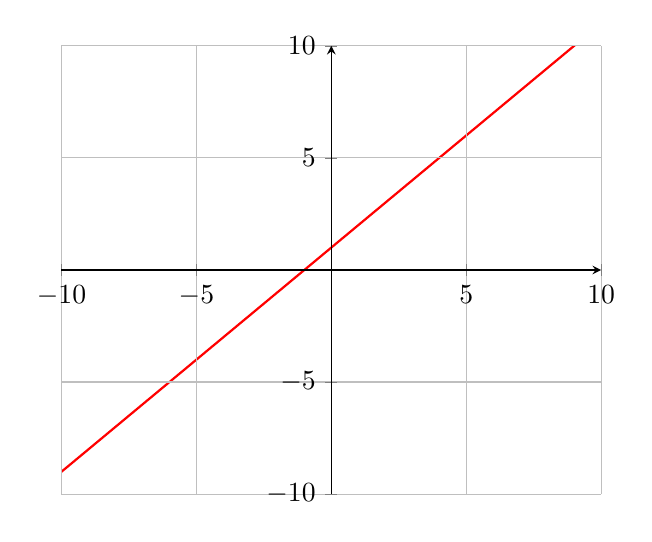
\begin{tikzpicture}
\begin{axis}[
	grid= major,
    xmin=-10, xmax=10,
    ymin=-10, ymax=10,
    axis lines=center,
    axis on top=true,
    domain=-10:10,
    ]

    \addplot [mark=none,draw=red, thick] {x+1};
\end{axis}
\end{tikzpicture}
\end{itemize}
\end{solution}

\begin{solution}
$f(x)=x-3$
\begin{itemize}
\item Pente :	$a=1$
\item Ordonnée à l’origine :	$x=0\Rightarrow f(x)=-3$
\item Zéro de fonction :	$f(x)=0\Rightarrow x=3$
\item Signe :	
$$\begin{array}{l|l|l|l|l|l}
x    & -\infty &   & 3 &   & +\infty \\
\hline
f(x) & -       & - & 0  & + & +      \\
& -\infty & \nearrow & \nearrow & \nearrow & +\infty \\   
\end{array}$$
\item Graphique
\begin{tikzpicture}
\begin{axis}[
    xmin=-10, xmax=10,
    ymin=-10, ymax=10,
    axis lines=center,
    axis on top=true,
    domain=-10:10,
    ]

    \addplot [mark=none,draw=red, thick] {x-3};
\end{axis}
\end{tikzpicture}
\end{itemize}
\end{solution}

\begin{solution}
$f(x)=2x-3$
\begin{itemize}
\item Pente :	$a=2$
\item Ordonnée à l’origine :	$x=0\Rightarrow f(x)=-3$
\item Zéro de fonction :	$f(x)=0\Rightarrow x=\frac{3}{2}$
\item Signe :	
$$\begin{array}{l|l|l|l|l|l}
x    & -\infty &   & \frac{3}{2} &   & +\infty \\
\hline
f(x) & -       & - & 0  & + & +      
\end{array}$$
\item Graphique
\begin{tikzpicture}
\begin{axis}[
    xmin=-10, xmax=10,
    ymin=-10, ymax=10,
    axis lines=center,
    axis on top=true,
    domain=-10:10,
    ]

    \addplot [mark=none,draw=red, thick] {2*x-3};
\end{axis}
\end{tikzpicture}
\end{itemize}
\end{solution}

\begin{solution}
$f(x)=2x+5$
\begin{itemize}
\item Pente :	$a=2$
\item Ordonnée à l’origine :	$x=0\Rightarrow f(x)=5$
\item Zéro de fonction :	$f(x)=0\Rightarrow x=-\frac{5}{2}$
\item Signe :	
$$\begin{array}{l|l|l|l|l|l}
x    & -\infty &   & -\frac{5}{2} &   & +\infty \\
\hline
f(x) & -       & - & 0  & + & +   \\
 & -\infty & \nearrow & \nearrow & \nearrow & +\infty \\   
\end{array}$$
\item Graphique
\begin{tikzpicture}
\begin{axis}[
    xmin=-10, xmax=10,
    ymin=-10, ymax=10,
    axis lines=center,
    axis on top=true,
    domain=-10:10,
    ]

    \addplot [mark=none,draw=red, thick] {2*x+5};
\end{axis}
\end{tikzpicture}
\end{itemize}
\end{solution}

\begin{solution}
$f(x)=\frac{x}{2}+1$
\begin{itemize}
\item Pente :	$a=\frac{1}{2}$
\item Ordonnée à l’origine :	$x=0\Rightarrow f(x)=1$
\item Zéro de fonction :	$f(x)=0\Rightarrow x=-2$
\item Signe :	
$$\begin{array}{l|l|l|l|l|l}
x    & -\infty &   & -2 &   & +\infty \\
\hline
f(x) & -       & - & 0  & + & +   \\
 & -\infty & \nearrow & \nearrow & \nearrow & +\infty \\   
\end{array}$$
\item Graphique
\begin{tikzpicture}
\begin{axis}[
    xmin=-10, xmax=10,
    ymin=-10, ymax=10,
    axis lines=center,
    axis on top=true,
    domain=-10:10,
    ]

    \addplot [mark=none,draw=red, thick] {x/2+1};
\end{axis}
\end{tikzpicture}
\end{itemize}
\end{solution}

\begin{solution}
$f(x)=-x+1$
\begin{itemize}
\item Pente :	$a=-1$
\item Ordonnée à l’origine :	$x=0\Rightarrow f(x)=1$
\item Zéro de fonction :	$f(x)=0\Rightarrow x=1$
\item Signe :
$$\begin{array}{l|l|l|l|l|l}
x    & -\infty &   & 1 &   & +\infty \\
\hline
f(x) & +       & + & 0  & - & -   \\
 & +\infty & \searrow & \searrow & \searrow & -\infty \\   
\end{array}$$
\item Graphique
\begin{tikzpicture}
\begin{axis}[
    xmin=-10, xmax=10,
    ymin=-10, ymax=10,
    axis lines=center,
    axis on top=true,
    domain=-10:10,
    ]

    \addplot [mark=none,draw=red, thick] {-x+1};
\end{axis}
\end{tikzpicture}
\end{itemize}
\end{solution}

\begin{solution}
$f(x)=-x-3$
\begin{itemize}
\item Pente :	$a=-1$
\item Ordonnée à l’origine :	$x=0\Rightarrow f(x)=-3$
\item Zéro de fonction :	$f(x)=0\Rightarrow x=-3$
\item Signe :	
$$\begin{array}{l|l|l|l|l|l}
x    & -\infty &   & -3 &   & +\infty \\
\hline
f(x) & +       & + & 0  & - & -   \\
 & +\infty & \searrow & \searrow & \searrow & -\infty \\   
\end{array}$$
\item Graphique
\begin{tikzpicture}
\begin{axis}[
    xmin=-10, xmax=10,
    ymin=-10, ymax=10,
    axis lines=center,
    axis on top=true,
    domain=-10:10,
    ]

    \addplot [mark=none,draw=red, thick] {-x-3};
\end{axis}
\end{tikzpicture}
\end{itemize}
\end{solution}

\begin{solution}
$f(x)=-2x-3$
\begin{itemize}
\item Pente :	$a=-2$
\item Ordonnée à l’origine :	$x=0\Rightarrow f(x)=-3$
\item Zéro de fonction :	$f(x)=0\Rightarrow x=-\frac{3}{2}$
\item Signe :	
$$\begin{array}{l|l|l|l|l|l}
x    & -\infty &   & -\frac{3}{2} &   & +\infty \\
\hline
f(x) & +       & + & 0  & - & -   \\
 & +\infty & \searrow & \searrow & \searrow & -\infty \\   
\end{array}$$
\item Graphique
\begin{tikzpicture}
\begin{axis}[
    xmin=-10, xmax=10,
    ymin=-10, ymax=10,
    axis lines=center,
    axis on top=true,
    domain=-10:10,
    ]

    \addplot [mark=none,draw=red, thick] {-2*x-3};
\end{axis}
\end{tikzpicture}
\end{itemize}
\end{solution}

\begin{solution}
$f(x)=5x+8$
\begin{itemize}
\item Pente :	$a=5$
\item Ordonnée à l’origine :	$x=0\Rightarrow f(x)=8$ 
\item Zéro de fonction :	$f(x)=0\Rightarrow x=-\frac{8}{5}$
\item Signe :
$$\begin{array}{l|l|l|l|l|l}
x    & -\infty &   & -\frac{8}{5} &   & +\infty \\
\hline
f(x) & -       & - & 0  & + & +   \\
 & -\infty & \nearrow & \nearrow & \nearrow & +\infty \\   
\end{array}$$
\item Graphique
\begin{tikzpicture}
\begin{axis}[
    xmin=-10, xmax=10,
    ymin=-10, ymax=10,
    axis lines=center,
    axis on top=true,
    domain=-10:10,
    ]

    \addplot [mark=none,draw=red, thick] {5*x+8};
\end{axis}
\end{tikzpicture}
\end{itemize}
\end{solution}

\begin{solution}
$f(x)=\frac{2x}{5}-3$
\begin{itemize}
\item Pente :	$a=\frac{2}{5}$
\item Ordonnée à l’origine :	$x=0\Rightarrow f(x)=-3$ 
\item Zéro de fonction :	$f(x)=0\Rightarrow x=\frac{15}{2}$
\item Signe :
$$\begin{array}{l|l|l|l|l|l}
x    & -\infty &   & -\frac{15}{2} &   & +\infty \\
\hline
f(x) & -       & - & 0  & + & +   \\
 & -\infty & \nearrow & \nearrow & \nearrow & +\infty \\   
\end{array}$$
\item Graphique
\begin{tikzpicture}
\begin{axis}[
    xmin=-10, xmax=10,
    ymin=-10, ymax=10,
    axis lines=center,
    axis on top=true,
    domain=-10:10,
    ]

    \addplot [mark=none,draw=red, thick] {2*x/5-3};
\end{axis}
\end{tikzpicture}
\end{itemize}
\end{solution}

\begin{solution}
$f(x)=5x-5$
\begin{itemize}
\item Pente :	$a=5$
\item Ordonnée à l’origine :	$x=0\Rightarrow f(x)=-5$ 
\item Zéro de fonction :	$f(x)=0\Rightarrow x=1$
\item Signe :
$$\begin{array}{l|l|l|l|l|l}
x    & -\infty &   & 1 &   & +\infty \\
\hline
f(x) & -       & - & 0  & + & +   \\
 & -\infty & \nearrow & \nearrow & \nearrow & +\infty \\   
\end{array}$$
\item Graphique
\begin{tikzpicture}
\begin{axis}[
    xmin=-10, xmax=10,
    ymin=-10, ymax=10,
    axis lines=center,
    axis on top=true,
    domain=-10:10,
    ]

    \addplot [mark=none,draw=red, thick] {5*x-5};
\end{axis}
\end{tikzpicture}
\end{itemize}
\end{solution}

\begin{solution}
$f(x)=-10x+3$
\begin{itemize}
\item Pente :	$a=-10$
\item Ordonnée à l’origine :	$x=0\Rightarrow f(x)=3$
\item Zéro de fonction :	$f(x)=0\Rightarrow x=\frac{3}{10}$
\item Signe :	
$$\begin{array}{l|l|l|l|l|l}
x    & -\infty &   & \frac{3}{10} &   & +\infty \\
\hline
f(x) & +       & + & 0  & - & -   \\
 & +\infty & \searrow & \searrow & \searrow & -\infty \\   
\end{array}$$
\item Graphique
\begin{tikzpicture}
\begin{axis}[
    xmin=-10, xmax=10,
    ymin=-10, ymax=10,
    axis lines=center,
    axis on top=true,
    domain=-10:10,
    ]

    \addplot [mark=none,draw=red, thick] {-10*x+3};
\end{axis}
\end{tikzpicture}
\end{itemize}
\end{solution}

\begin{solution}
$f(x)=-3x+7$
\begin{itemize}
\item Pente :	$a=-3$
\item Ordonnée à l’origine :	$x=0\Rightarrow f(x)=7$
\item Zéro de fonction :	$f(x)=0\Rightarrow x=\frac{7}{3}$
\item Signe :
$$\begin{array}{l|l|l|l|l|l}
x    & -\infty &   & \frac{7}{3} &   & +\infty \\
\hline
f(x) & +       & + & 0  & - & -   \\
 & +\infty & \searrow & \searrow & \searrow & -\infty \\   
\end{array}$$
\item Graphique
\begin{tikzpicture}
\begin{axis}[
    xmin=-10, xmax=10,
    ymin=-10, ymax=10,
    axis lines=center,
    axis on top=true,
    domain=-10:10,
    ]

    \addplot [mark=none,draw=red, thick] {-3*x+7};
\end{axis}
\end{tikzpicture}
\end{itemize}
\end{solution}

\begin{solution}
$f(x)=\frac{3}{8}x-2$
\begin{itemize}
\item Pente :	$a=\frac{3}{8}$
\item Ordonnée à l’origine :	$x=0\Rightarrow f(x)=-2$ 
\item Zéro de fonction :	$f(x)=0\Rightarrow x=\frac{16}{3}$
\item Signe :	
$$\begin{array}{l|l|l|l|l|l}
x    & -\infty &   & \frac{16}{3} &   & +\infty \\
\hline
f(x) & -       & - & 0  & + & +   \\
 & -\infty & \nearrow & \nearrow & \nearrow & +\infty \\   
\end{array}$$
\item Graphique
\begin{tikzpicture}
\begin{axis}[
    xmin=-10, xmax=10,
    ymin=-10, ymax=10,
    axis lines=center,
    axis on top=true,
    domain=-10:10,
    ]

    \addplot [mark=none,draw=red, thick] {3*x/8-2};
\end{axis}
\end{tikzpicture}
\end{itemize}
\end{solution}

\begin{solution}
$f(x)=-\frac{x}{8}-1$
\begin{itemize}
\item Pente :	$a=-\frac{1}{8}$
\item Ordonnée à l’origine :	$x=0\Rightarrow f(x)=-1$
\item Zéro de fonction :	$f(x)=0\Rightarrow x=-8$
\item Signe :	
$$\begin{array}{l|l|l|l|l|l}
x    & -\infty &   & -8 &   & +\infty \\
\hline
f(x) & +       & + & 0  & - & -   \\
 & +\infty & \searrow & \searrow & \searrow & -\infty \\   
\end{array}$$
\item Graphique
\begin{tikzpicture}
\begin{axis}[
    xmin=-10, xmax=10,
    ymin=-10, ymax=10,
    axis lines=center,
    axis on top=true,
    domain=-10:10,
    ]

    \addplot [mark=none,draw=red, thick] {-x/8-1};
\end{axis}
\end{tikzpicture}
\end{itemize}
\end{solution}

\begin{solution}
$f(x)=5$
\begin{itemize}
\item Pente :	$a=0$
\item Ordonnée à l’origine :	$x=0\Rightarrow f(x)=5$
\item Zéro de fonction :	$f(x)=0\Rightarrow x=\pm \infty $
\item Signe :	$$\begin{array}{l|l|l|l|l|l}
x    & -\infty &   & &   & +\infty \\
\hline
f(x) & +       & + & +  & + & +   \\
 & 5 & \rightarrow & \rightarrow & \rightarrow & 5 \\   
\end{array}$$
\item Graphique
\begin{tikzpicture}
\begin{axis}[
    xmin=-10, xmax=10,
    ymin=-10, ymax=10,
    axis lines=center,
    axis on top=true,
    domain=-10:10,
    ]

    \addplot [mark=none,draw=red, thick] {5};
\end{axis}
\end{tikzpicture}
\end{itemize}
\end{solution}

\begin{solution}
$f(x)=-4$
\begin{itemize}
\item Pente :	$a=0$
\item Ordonnée à l’origine :	$x=0\Rightarrow f(x)=-4$
\item Zéro de fonction :	$f(x)=0\Rightarrow x=\pm \infty $
\item Signe :	$$\begin{array}{l|l|l|l|l|l}
x    & -\infty &   & &   & +\infty \\
\hline
f(x) & -       & - & -  & - & -   \\
 & -4 & \rightarrow & \rightarrow & \rightarrow & -4 \\   
\end{array}$$
\item Graphique
\begin{tikzpicture}
\begin{axis}[
    xmin=-10, xmax=10,
    ymin=-10, ymax=10,
    axis lines=center,
    axis on top=true,
    domain=-10:10,
    ]

    \addplot [mark=none,draw=red, thick] {-4};
\end{axis}
\end{tikzpicture}
\end{itemize}
\end{solution}

\begin{solution}
$f(x)=3x$
\begin{itemize}
\item Pente :	$a=3$
\item Ordonnée à l’origine :	$x=0\Rightarrow f(x)=0$ 
\item Zéro de fonction :	$f(x)=0\Rightarrow x=0$
\item Signe :	$$\begin{array}{l|l|l|l|l|l}
x    & -\infty &   & 0 &   & +\infty \\
\hline
f(x) & -       & - & 0  & + & +   \\
 & -\infty & \nearrow & \nearrow & \nearrow & +\infty \\   
\end{array}$$
\item Graphique
\begin{tikzpicture}
\begin{axis}[
    xmin=-10, xmax=10,
    ymin=-10, ymax=10,
    axis lines=center,
    axis on top=true,
    domain=-10:10,
    ]

    \addplot [mark=none,draw=red, thick] {3*x};
\end{axis}
\end{tikzpicture}
\end{itemize}
\end{solution}

\begin{solution}
$f(x)=-6x$
\begin{itemize}
\item Pente :	$a=-6$
\item Ordonnée à l’origine :	$x=0\Rightarrow f(x)=0$
\item Zéro de fonction :	$f(x)=0\Rightarrow x=0$
\item Signe :	$$\begin{array}{l|l|l|l|l|l}
x    & -\infty &   & 0 &   & +\infty \\
\hline
f(x) & +       & + & 0  & - & -   \\
 & +\infty & \searrow & \searrow & \searrow & -\infty \\   
\end{array}$$
\item Graphique
\begin{tikzpicture}
\begin{axis}[
    xmin=-10, xmax=10,
    ymin=-10, ymax=10,
    axis lines=center,
    axis on top=true,
    domain=-10:10,
    ]

    \addplot [mark=none,draw=red, thick] {-6*x};
\end{axis}
\end{tikzpicture}
\end{itemize}
\end{solution}

\begin{solution}
$f(x)=\frac{5}{7}x$
\begin{itemize}
\item Pente :	$a=\frac{5}{7}$
\item Ordonnée à l’origine :	$x=0\Rightarrow f(x)=0$ 
\item Zéro de fonction :	$f(x)=0\Rightarrow x=0$
\item Signe :	$$\begin{array}{l|l|l|l|l|l}
x    & -\infty &   & 0 &   & +\infty \\
\hline
f(x) & -       & - & 0  & + & +   \\
 & -\infty & \nearrow & \nearrow & \nearrow & +\infty \\   
\end{array}$$
\item Graphique
\begin{tikzpicture}
\begin{axis}[
    xmin=-10, xmax=10,
    ymin=-10, ymax=10,
    axis lines=center,
    axis on top=true,
    domain=-10:10,
    ]

    \addplot [mark=none,draw=red, thick] {5*x/7};
\end{axis}
\end{tikzpicture}
\end{itemize}
\end{solution}

% ok / corrigé ok

% \chapter{Seuil de rentablité}

Ce chapitre sera consacré à l'étude de problèmes financiers.

\section{Recherche de seuil}

Nous nous intéresserons ici aux entreprises qui produisent un seul article. Pour pouvoir en fabriquer en quantité, elles ont un certain nombre de frais.

Des frais sont liés à l'existence de l'entreprise (local à louer, machines à acheter, etc.) et d'autres à la production (matière première, etc). On appelle les premiers les \emph{frais fixes}\index{seuil de rentabilité!frais fixes}, notés $f_f$ et les second les \emph{frais variables}\index{seuil de rentabilité!frais variables}, notés $f_v$. Bien entendu, les frais fixes ne dépendent pas du nombre d'objets produits, alors que les second oui.

Secondement, l'entreprise vend ses produits, ce qui génère un \emph{gain}\index{seuil de rentabilité!gain}, noté $g$. L'ensemble des gains pour la vente de toute la production est ce qu'on appelle en économie le chiffre d'affaire. Dans tout ce chapitre, nous considérerons que l'ensemble de la production est systématiquement vendue.

Le \emph{seuil de rentabilité}\index{seuil de rentabilité} est le nombre d'objet qu'il faut produire afin d'équilibrer les gains et les frais. Il se trouve en résolvant l'équation

$$
f_v \cdot x + f_f = g\cdot x
$$
où $x$ est le nombre de marchandise produite. La fonction $f_v + f_f \cdot x$ représente l'ensemble des frais de l'entreprise pour produire $x$ marchandise, alors que la fonction $g\cdot x$ l'ensemble des gains liés à la vente de $x$ marchandises.

\begin{exemple}\label{ex_seuil}
Mon amie décide de se lancer dans la production de scoubidous. Pour cela, elle doit acheter une tresseuse de scoubidous à $100$ Frs. Elle a calculé que chaque scoubidou lui coûte $0.50$ Frs de fil. Enfin, elle décide de les vendre $3$ Frs pièce. Quel est sont seuil de rentabilité ?

En analysant le problème, on trouve :
$$
\left\{
\begin{array}{l}
f_f = 100\\
f_v = 0.5
g = 3
\end{array}
\right.
\Rightarrow
\left\{
\begin{array}{l}
f(x) = 0.5 x + 100\\
g(x) = 3x
\end{array}
\right.
$$
On doit donc résoudre l'équation
$$
\begin{array}{lcl}
0.5 x + 100 &=& 3x \ssi \\
100 &=& 2.5 x \ssi \\
40 &=& x
\end{array}
$$
Son seuil de rentabilité est donc de $40$ pièces, c'est-à-dire que si elle en produit moins elle perd de l'argent, et elle commence à en gagner à $41$ pièces.
\end{exemple}

\subsection{Représentation}

On vient de le voir, la situation peut être explicitée sous la forme de deux fonctions :
$$
\begin{array}{l}
f(x) = f_v \cdot c + f_f \mbox{ (les frais)}\\
g(x) = g\cdot x \mbox{ (les gains)}
\end{array}
$$

Or il s'agit de deux fonctions affines dont nous avons parlé à la section~\ref{fct_affine}. Puisque $x$ ne peut être que positif (il est peu probable de produite un nombre négatif de marchandise) et que les images des nombres positifs par $f$ et $g$ sont aussi positives, nous nous contenterons de représenter la situation dans le premier cadran, c'est-à-dire le quart supérieur droite.

Le seuil de rentabilité est le moment où $f(x) = g(x)$, et donc les deux graphes passent par le point $\left(x;f(x)\right) = \left(x;g(x)\right)$. Ainsi, puisque les deux droites passent par ce point, elle se coupent au seuil de rentabilité.

Pour une représentation un peu précise, il convient de représenter chaque droite en utilisant l'image de $0$ (l'ordonnée à l'origine) et l'image d'un nombre suffisamment grand (en général, deux fois le seuil de rentabilité).

\begin{exemple}
Reprenons l'exemple~\ref{ex_seuil} : nous avons les deux fonction suivantes :
$$
\left\{
\begin{array}{l}
f(x) = 0.5 x + 100\\
g(x) = 3x
\end{array}
\right.
$$
On sait déjà que le seuil est à $40$ pièces, nous allons donc calculer les images de $0$ et de $80$ :
$$
\left\{
\begin{array}{l}
f(0) = 0.5 \cdot 0 + 100 = 100 \Rightarrow (0;100)\\
g(0) = 3\cdot 0 = 0 \Rightarrow (0;0)
\end{array}
\right.
\mbox{ et }
\left\{
\begin{array}{l}
f(80) = 0.5 \cdot 80 + 100 = 140 \Rightarrow (0;140)\\
g(80) = 3\cdot 80 =240 \Rightarrow (0;240)
\end{array}
\right.
$$
On représente donc la situation ainsi :
\begin{center}
\includegraphics[width=0.7\textwidth]{rentabilite/seuil_ex.png}
\end{center}
Pour faciliter la représentation, il est souvent nécessaire de ne pas utiliser la même graduation pour les deux axes !
\end{exemple}

\section{Comparatif d'offres}

Cette section peut paraître n'avoir aucun lien avec le chapitre, mais le raisonnement est le même que pour les seuil de rentabilités.

On s'intéresse ici à plusieurs offres portant sur la même matière (par exemple : payer tous ses  trajets, prendre un demi-tarif ou un abonnement général) et on cherche à analyser l'offre. Par exemple, à partir de combien de trajet prendre un demi tarif est-il plus avantageux que de payer en plein chaque déplacement ?

Pour cela, nous allons commencer par décrire la fonction liée à chaque offre, représenter son graphe et nous intéresser aux points d'intersection (on commence à voir le rapport avec le seuil de rentabilité).

\begin{exemple}
Jean-Paul fait régulièrement le trajet Martigny-Genève. Il paye son billet $41$ Frs. Le demi-tarif est à $185$ Frs par année et l'abonnement général à $3655$ Frs par année. Que conseiller à Jean-Paul ?

Soit $x$ le nombre de trajets que Jean-Paul effectue par année, $h(x)$ ce qu'il paye avec des billets normaux, $i(x)$ avec le demi-tarif et $j(x)$ avec l'abonnement général. On peut assez vite deviner :
$$
\left\{
\begin{array}{l}
h(x) = 41 x\\
i(x) = \frac{41}{2} x + 185\\
j(x) = 3655
\end{array}
\right.
$$
On fait donc le graphique suivant :
\begin{center}
\includegraphics[width = 0.9 \textwidth]{rentabilite/comparatif.png}
\end{center}
Ainsi dans la première zone, la fonction $h$ est la plus avantageuse, la deuxième, la fonction $i$ et la dernière la fonction $j$.

Il nous faut à présent trouver les pivots des zones. On les trouve aux intersections des fonction $h$ et $i$ ainsi qu'à celle des fonctions $i$ et $j$. L'intersection des fonction $h$ et $j$ ne nous intéresse pas, comme on le voit sur le graphique.

Commençons par les fonctions $h$ et $i$ :
$$
\begin{array}{lcl}
41 x &=& \frac{41}{2} x + 185 \ssi \\
41x - \frac{41}{2}x = 185 \ssi \\
\frac{41}{2} x = 185 \ssi \\
x = \frac{370}{41} \simeq 9,02
\end{array}
$$
puis par celle des fonctions $i$ et $j$
$$
\begin{array}{lcl}
\frac{41}{2}x + 185 &=& 3655 \ssi \\
\frac{41}{2} x &=& 3470 \ssi \\
x = \frac{6940}{41} \simeq 169,27
\end{array}
$$
Ainsi si Jean-Paul effectue entre $0$ et $9$ trajets par an, il préférera payer ses trajets en plein, entre $10$ et $169$ trajets, il prendra un demi-tarif, au-delà de $170$ trajets, il prendra un abonnement général.
\end{exemple}% ok / corrige ok

\chapter{Droite dans le plan}\label{droite_plan}

\section{Rappel}

Commençons par rappeler la définition du plan et des notions associées :

\begin{definition}
Le \emph{plan}\index{plan} est l'ensemble des couples $(x;y)$ avec $x,y\in \R$. On peut ainsi le représenter comme une feuille infinie.

Pour s'y repérer, nous utiliserons deux axes gradués, perpendiculaires et se croisant sur le point $(0;0)$.

Le premier axe, horizontal, s'appelle l'\emph{abscisse}\index{abscisse} et le second, vertical, l'\emph{ordonnée}\index{ordonnée}. Le point $(0;0)$, quant à lui, s'appelle l'\emph{origine}\index{origine}.
\end{definition}

\begin{center}
\includegraphics[width = 0.9 \textwidth]{droite/plan.png}
\end{center}

Sur le plan, tout point peut être représenté selon ses deux coordonnées $x$ et $y$ comme nous l'avons vu à la section~\ref{fct_representation}.

Aussi, de manière générale, nous parlerons du point
$$
P(x_P;y_P)
$$

Par exemple, pour le point $A(3;-2)$, on a $x_A = 3$ et $y_A = -2$. Cette notion est très importante et nous l'utiliserons dans tout ce chapitre !

\section{Droite}

Euclide\index{Euclide}, en $300$ avant J.-C., écrivait à propos de la droite :
\begin{quote}
\begin{enumerate}
\item Une ligne est une longueur sans largeur.\label{def_droite}
\item  Un segment de droite peut être tracé en joignant deux points quelconques.\label{elt_un}
\item Un segment de droite peut être prolongé indéfiniment en une ligne droite.\label{elt_deux}
\item Étant donné un segment de droite quelconque, un cercle peut être tracé en prenant ce segment comme rayon et l'une de ses extrémités comme centre.\label{elt_trois}
\item Tous les angles droits sont congruents.\label{elt_quatre}
\item Si deux lignes droites sont sécantes avec une troisième de telle façon que la somme des angles intérieurs d'un côté est inférieure à deux angles droits, alors ces deux lignes sont forcément sécantes de ce côté.\label{elt_cinq}
\end{enumerate}
\end{quote}
Pour nous, seule les éléments~(\ref{def_droite}), (\ref{elt_un}) et (\ref{elt_deux}) concernent la droite. Mais il est intéressant de voir que ces notions intéressaient les grecs déjà dans l'antiquité. C'est aussi dans l'histoire l'une des premières fois que la notion d'infini appara\^it.

Pour nous, nous définirons la notion de droite via la \emph{géométrie analytique} :

\begin{definition}
Une \emph{droite} est un ensemble de point vérifiant une équation à deux inconnues linéaire du type
$$\begin{array}{l}
ax+by=c, \mbox{ avec } a,b,c\in \R \mbox{ forme implicite}\\
y = mx + h, \mbox{ avec } m,h\in \R \mbox{ forme explicite}
\end{array}
$$
\end{definition}

Remarquons dans cette définition que la forme explicite ressemble fortement à une fonction affine (section~\ref{fct_affine}). Nous utiliserons des notions de fonction pour les droites par la suite.

On voit peu le lien entre cette définition et l'idée, toute simple, que l'on peut se faire d'une droite. Voyons cela de plus près avec un exemple :

\begin{exemple}
Soit la droite $d:2x+5y = 10$. Une première question serait : comment savoir si un point $P$ est sur la droite $d$. Prenons donc un point $P(3;2)$ au hasard. Pour savoir si $P$ est sur la droite, il convient d'appliquer l'équation de la droite au point :
$$
\begin{array}{rcl}
P &\in^?& d \ssi \\
d:2x_P + 5y_P &=^?& 10\ssi \\
2\cdot 3 + 5 \cdot 2 &=^?& 10 \ssi \\
6 + 10 &=^?& 10 \ssi \\
16 &=^?& 10
\end{array}
$$
Puisque manifestement $16\neq 10$, le point $P$ n'est pas sur la droite $d$.

Dès lors, comment trouver un point qui est sur la droite $d$ ? Puisque nous avons une seule équation et deux inconnues, nous pouvons sans problème fixer une coordonnée, c'est-à-dire attribuer une valeur au hasard à $x$ ou à $y$. Pour simplifier les calculs, commençons par poser $x=0$ :
$$
\begin{array}{lcl}
2 \cdot 0 + 5 y &=& 10 \ssi \\
5y  &=& 10 \ssi \\
y &=& 2.
\end{array}
$$
Ainsi puisque nous avons posé $x=0$ et que nous avons trouvé $y=2$, la droite $d$ passe par le point $A(0;2)$. C'est déjà un début, mais pour rejoindre le point de vue d'Euclide sur la droite, il nous faut un deuxième point. Naturellement regardons ce qui se passe si $y=0$ :
$$
\begin{array}{lcl}
2x + 5\cdot 0 &=& 10 \ssi \\
2x &=& 10 \ssi \\
x &=& 5.
\end{array}
$$
Ainsi puisque nous avons posé $y=0$ et que nous avons trouvé $x=5$, la droite $d$ passe par le point $B(5;0)$. Si on devait la dessiner, on trouverait :
\begin{center}
\includegraphics[width = 0.9\textwidth]{droite/droite_ex.png}
\end{center}
On remarque que la droite passe aussi par le point $C(10;-2)$, mais est-ce que ce point vérifie l'équation de la droite $d$ ?
$$
\begin{array}{rcl}
C &\in^?& d \ssi \\
d:2x_C + 5y_C &=^?& 10\ssi \\
2\cdot 10 + 5 \cdot (-2) &=^?& 10 \ssi \\
20 - 10 &=^?& 10 \ssi \\
10 &=^?& 10
\end{array}
$$
Puisque manifestement $10 = 10$, le point $C$ est sur la droite $d$. Or il en est de même pour les autres points de la droite et l'on voit ainsi comment les notions d'Euclide et de géométrie analytique se rejoignent.
\end{exemple}

Intéressons-nous maintenant à une notion déjà aperçue dans la section des fonctions affines : la pente.

\begin{definition}
La \emph{pente}\index{pente!d'une droite} entre deux points $A$ et $B$ du plan est donnée par 
$$
\mbox{pente } = \frac{\mbox{distance verticale entre }A\mbox{ et }B}{\mbox{distance horizontale entre }A\mbox{ et }B}
$$
\end{definition}

Comme on le voit sur le graphique suivant, la pente d'une droite est donnée par la formule
$$
\mbox{pente } = \frac{y_B-y_A}{x_B-x_A}
$$

\begin{center}
\includegraphics[width=0.9 \textwidth]{droite/droite_pente.png}
\end{center}

\begin{theoreme}
La pente d'une droite est donnée par $m$ dans sa forme explicite.
\end{theoreme}

\begin{proof}
Soit une droite $d:y = mx+h$ et soient $A$ et $B$ deux points sur la droite. Ainsi
$$
\left\{
\begin{array}{lcl}
y_A &=& mx_A + h\\
y_B &=& mx_B + h
\end{array}
\right.
$$
Si l'on soustrait ces deux équations et que l'on isole $m$ on obtient :
$$
\begin{array}{lcl}
y_B-y_A &=& (mx_B + h)-(mx_A + h)\ssi \\
y_B-y_A &=& mx_B + h-mx_A - h\ssi \\
y_B-y_A &=& mx_B-mx_A \ssi \\
(y_B-y_A) &=& m(x_B-x_A)\ssi \\
\frac{(y_B-y_A)}{(x_B-x_A)} &=& m\ssi \\
\end{array}
$$
ce qui démontre que $m$ est la pente de la droite $d$.
\end{proof}

\subsection{Parallèle}

En géométrie euclidienne, on dit que deux droites sont parallèles si et seulement si elles n'ont aucune intersection. Avec le postulat~(\ref{elt_cinq}) que l'on trouve au début de ce chapitre on peut conclure que par un point passe une seule parallèle à une autre droite. Cette notion parait tellement triviale que durant longtemps les mathématiciens ont essayé de la démontrer. Euler~\index{Euler}, un mathématicien suisse du 18e siècle a proposé d'autres modèles de géométrie, typiquement la géométrie sur une sphère, où cette propriété n'est pas vérifiée (c'est-à-dire qu'on peut faire passer plusieurs parallèles par le même point).

\begin{proposition}
En géométrie euclidienne, deux droites sont parallèles si et seulement si elles ont la même pente.
\end{proposition}

Cette proposition ne sera pas démontrée, une compréhension graphique suffit.

\subsection{Perpendiculaires}

La notion de perpendiculaire est, au sein de notre progression, difficile à définir. En effet, nous n'avons pas défini la notion d'angle. Aussi nous considérerons la notion de perpendicularité comme intuitive, par exemple s'il est possible de dessiner un carré ayant chacune des deux droites sécantes comme diagonales.

\begin{proposition}
Soient $d_1$ et $d_2$ deux droites ayant respectivement les pentes $m_1$ et $m_2$. Alors les deux droites sont perpendiculaires si et seulement si
$$
m_1 = \frac{-1}{m_2}.
$$
\end{proposition}

\begin{proof}
Voyons cette proposition par voie graphique et uniquement dans un sens :
\begin{center}
\includegraphics[width=0.9\textwidth]{droite/perpendiculaire.png}
\end{center}
On remarque que la verticale de $d_2$ est égale à l'horizontale de $d_1$ et que l'horizontale de $d_2$ est le contraire de la verticale de $d_1$.
Ainsi 
$$
\begin{array}{lcl}
m_1 &=& \frac{\mbox{vertical}_1}{\mbox{horizontal}_1}\\
&=& \frac{-\mbox{horizontal}_2}{\mbox{vertical}_2}\\
&=& \frac{-1}{\frac{\mbox{vertical}_2}{\mbox{horizontal}_2}}\\
&=& \frac{-1}{m_2}.
\end{array}
$$
Une partie de la proposition est ainsi démontrée. Il nous faudrait encore voir que si deux droites respectent l'égalité liée aux pentes, alors elles sont perpendiculaires, mais comme notre définition de perpendiculaire est très intuitive, elle complique la démonstration.
\end{proof}

\section{Exercices}

\begin{exercice}
\'Etudier toutes les caractéristiques des droites suivantes (formes implicites).
	Tracer au maximum deux droites sur un même système d'axes, unité des axes : un carré.
\begin{multicols}{2}
\begin{enumerate}
\item $x+y=5$
\item $x-y=-3$
\item $2x+y=6$
\item $x-3y=12$
\item $3x+2y=6$
\item $-2x+3y=6$
\item $-3x-5y=30$
\item $5x+2y=-20$
\item $7x-2y=-28$
\item $3x-4y=9$
\item $-4x+5y=-15$
\item $2x+3y=5$
\item $y=-4$
\item $5y=35$
\item $x=6$
\item $-3x=12$
\end{enumerate}
\end{multicols}
\end{exercice}

\begin{exercice}
Calculer les équations des droites suivantes, connaissant la pente p et les coordonnées d'un point A de la droite. Donner les formes explicites et implicites des équations de droites.
\begin{multicols}{2}
\begin{enumerate}
\item $p=1\text{     }A(1;2)$
\item $p=3\text{     }A(-1;3)$
\item $p=-4\text{     }A(5;-5)$
\item $p=-7\text{     }A(-4;-3)$
\item $p=\frac{1}{2}\text{     }A(4;12)$
\item $p=\frac{4}{5}\text{     }A(-9;5)$
\item $p=-\frac{8}{3}\text{     }A(0;3)$
\item $p=-\frac{11}{13}\text{     }A(-5;0)$
\item $p=\frac{127}{19}\text{     }A(0;0)$
\item $p=\frac{34}{11}\text{     }A(-7;15)$
\item $p=0\text{     }A(4;5)$
\item $p=\infty \text{     }A(4;5)$
\end{enumerate}
\end{multicols}
\end{exercice}

\begin{exercice}
Calculer les équations des droites suivantes, connaissant les coordonnées de deux points A et B de la droite. Donner les formes explicites et implicites des équations de droites.
\begin{multicols}{2}
\begin{enumerate}
\item $$ \left| \begin{array}{l}
 A(2;3) \\ 
B\left( 1;5 \right) \\ 
\end{array} \right.$$
\item $$\left| \begin{array}{l}
 A(12;7) \\ 
B\left( -2;5 \right) \\ 
\end{array} \right.$$
\item $$\left| \begin{array}{l}
 A(-11;-7) \\ 
B\left( 1;1 \right) \\ 
\end{array} \right.$$
\item $$\left| \begin{array}{l}
 A(5;7) \\ 
B\left( -3;-9 \right) \\ 
\end{array} \right.$$
\item $$\left| \begin{array}{l}
 A(-6;4) \\ 
B\left( 7;-2 \right) \\ 
\end{array} \right.$$
\item $$\left| \begin{array}{l}
 A(10;-12) \\ 
B\left( -4;5 \right) \\ 
\end{array} \right.$$
\item $$\left| \begin{array}{l}
 A(3,5;5,5) \\ 
B\left( 2,5;7,5 \right) \\ 
\end{array} \right.$$
\item $$\left| \begin{array}{l}
 A(75;-37) \\ 
B\left( -1;8 \right) 
 \end{array} \right.$$
\item $$\left| \begin{array}{l}
 A(5;5) \\ 
B\left( 12;12 \right) \\ 
\end{array} \right.$$
\item $$\left| \begin{array}{l}
 A(2;-6) \\ 
B\left( 6;-18 \right) \\ 
\end{array} \right.$$
\item $$\left| \begin{array}{l}
 A(3;7) \\ 
B\left( 15;7 \right) \\ 
\end{array} \right.$$
\item $$\left| \begin{array}{l}
 A(-2;-3) \\ 
B\left( -2;6 \right) \\ 
\end{array} \right.$$
\end{enumerate}
\end{multicols}
\end{exercice}

\begin{exercice}
Calculer les coordonnées du point M, milieu du segment AB.
\begin{multicols}{2}
\begin{enumerate}
\item $$\left| \begin{array}{l}
 A\left( 6;8 \right) \\ 
B\left( 2;12 \right) \\ 
\end{array} \right.$$
\item $$\left| \begin{array}{l}
 A\left( -4;16 \right) \\ 
B\left( 6;-10 \right) \\ 
\end{array} \right.$$
\item $$\left| \begin{array}{l}
 A\left( 5;11 \right) \\ 
B\left( 3;-9 \right) \\ 
\end{array} \right.$$
\item $$\left| \begin{array}{l}
 A\left( -18;77 \right) \\ 
B\left( 25;34 \right) \\ 
\end{array} \right.$$
\item $$\left| \begin{array}{l}
 A\left( \frac{13}{2};-\frac{3}{4} \right) \\ 
B\left( -\frac{7}{3};\frac{3}{5} \right) \\ 
\end{array} \right.$$
\item $$\left| \begin{array}{l}
 A\left( 0;0 \right) \\ 
B\left( -16;24 \right) \\ 
\end{array} \right.$$
\end{enumerate}
\end{multicols}
\end{exercice}

\begin{exercice}
Calculer la longueur du segment AB.
\begin{multicols}{3}
\begin{enumerate}
\item $$\left| \begin{array}{l}
 A\left( 2;10 \right) \\ 
B\left( 5;12 \right) \\ 
\end{array} \right.$$
\item $$\left| \begin{array}{l}
 A\left( -8;5 \right) \\ 
B\left( 6;-2 \right) \\ 
\end{array} \right.$$
\item $$\left| \begin{array}{l}
 A\left( 0;0 \right) \\ 
B\left( -5;0 \right) \\ 
\end{array} \right.$$
\end{enumerate}
\end{multicols}
\end{exercice}

\begin{exercice}
Calculer l'équation de la droite passant par le point A et parallèle à la droite d.
\begin{multicols}{3}
\begin{enumerate}
\item $$\left| \begin{array}{l}
 A\left( 5;9 \right) \\ 
d:y=3x-5 \\ 
\end{array} \right.$$
\item $$\left| \begin{array}{l}
 A\left( -3;4 \right) \\ 
d:y=-\frac{5x}{2}+1 \\ 
\end{array} \right.$$
\item $$\left| \begin{array}{l}
 A\left( -7;-3 \right) \\ 
d:3x+7y=2 \\ 
\end{array} \right.$$
\end{enumerate}
\end{multicols}
\end{exercice}

\begin{exercice}
Calculer l'équation de la droite passant par le point A et perpendiculaire à la droite d.
\begin{multicols}{3}
\begin{enumerate}
\item $$\left| \begin{array}{l}
 A\left( 3;-2 \right) \\ 
d:y=2x-5 \\ 
\end{array} \right.$$
\item $$\left| \begin{array}{l}
 A\left( -6;0 \right) \\ 
d:y=\frac{3x}{7} \\ 
\end{array} \right.$$
\item $$\left| \begin{array}{l}
 A\left( -3;8 \right) \\ 
d:5x+2y=2 \\ 
\end{array} \right.$$
\end{enumerate}
\end{multicols}
\end{exercice}

\section{Corrigés}

\begin{solution}

\end{solution}

\begin{landscape}

\begin{solution}
Calculer les équations des droites suivantes, connaissant la pente p et les coordonnées d'un point A de la droite. Donner les formes explicites et implicites des équations de droites.
$$
\begin{array}{|l|l|l|l|l|l|}
\hline
1.          & 2.           & 3.            & 4.            & 5.                   & 6.                                \\ \hline
p = 1       & p = 3        & p =-4       & p =-7       & p=\frac{1}{2}     & p=\frac{4}{5}                  \\ \hline
A(1 ;2)     & A(- 1 ;3)    & A(5 ;-5)    & A(- 4 ;- 3)   & A(4 ;12)             & A(- 9 ;5)                         \\ \hline
y = x+b     & y = 3x + b   & y =-4x + b  & y =-7 x + b & y=\frac{1}{2}x+b  & y=\frac{4}{5}x+b               \\ \hline
2 = 1 + b   & 3 =-3 + b  & -5 =-20 + b &-3 = 28 + b  & 12 = 2 + b           & 5=-\frac{36}{5}+b              \\ \hline
b = 1       & b = 6        & b = 15        & b = -31       & b = 10               & b=\frac{61}{5}                 \\ \hline
y = x + 1   & y = 3x + 6   & y =-4x + 15 & y = -7 x-31 & y=\frac{1}{2}x+10 & y=\frac{4}{5}x+\frac{61}{5} \\ \hline
x-y =-1 & 3x-y =-6 & 4x + y = 15   & 7x + y =-31 & x-2y =-20        & 4x-5y =-61                    \\ \hline
\end{array}
$$

$$
\begin{array}{|l|l|l|l|l|l|}
\hline
7.                   & 8.                                    & 9.                     & 10.                                   & 11.         & 12.                                                                            \\ \hline
p=-\frac{8}{3}    & p=-\frac{11}{13}                   & p=\frac{127}{19}    & p=\frac{34}{11}                    & p=0         & p=infty                                                                        \\ \hline
A(0 :3)              & A(- 5 ;0)                             & A(0 ;0)                & A(- 7 ;15)                            & A(4 ;5)     & A(4 ;5)                                                                        \\ \hline
y=-\frac{8}{3}x+b & y=-\frac{11}{13}x+b                & y=\frac{127}{19}x+b & y=\frac{34}{11}x+b                 & y=0x+b      & \begin{array}[c]{@{}l@{}}Droite verticale d’équation \\   x = 4\end{array} \\ \hline
3 = b                & 0=\frac{55}{13}+b                  &                        & 15=-\frac{238}{11}+b               & 5=0cdot 4+b &                                                                                \\ \hline
b = 3                & b=-\frac{55}{13}                   & b = 0                  & b=\frac{403}{11}                   & b=5         &                                                                                \\ \hline
y=-\frac{8}{3}x+3 & y=-\frac{11}{13}x-\frac{55}{13} & y=\frac{127}{19}x   & y=\frac{34}{11}x+\frac{403}{11} & y=5         &                                                                                \\ \hline
8x+3y=9              & 11x + 13y =-55                      & 127x-19y = 0         & 34x -11y = -403                       &             &                                                                                \\ \hline
\end{array}
$$
\end{solution}

\end{landscape}

\begin{solution}
Calculer les équations des droites suivantes, connaissant les coordonnées de deux points A et B de la droite. Donner les formes explicites et implicites des équations de droites.
$$
\begin{array}{|l|l|l|l|l|l|}
\hline
1.                                                          & 2.                                                             & 3.                                                               & 4.                                                              & 5.                                                              & 6.                                                                \\ \hline
\begin{array}[c]{@{}l@{}}A(2 ;3)\\   B(1 ;5)\end{array} & \begin{array}[c]{@{}l@{}}A(12 ;7)\\   B(- 2 ;5)\end{array} & \begin{array}[c]{@{}l@{}}A(- 11 ;- 7)\\   B(1 ;1)\end{array} & \begin{array}[c]{@{}l@{}}A(5 ;7)\\   B(- 3 ;- 9)\end{array} & \begin{array}[c]{@{}l@{}}A(- 6 ;4)\\   B(7 ;- 2)\end{array} & \begin{array}[c]{@{}l@{}}A(10 ;- 12)\\   B(- 4 ;5)\end{array} \\ \hline
a=\frac{5-3}{1-2}                                        & a=\frac{5-7}{-2-12}                                         & a=\frac{1+7}{1+11}                                            & a=\frac{-9-7}{-3-5}                                          & a=\frac{-2-4}{7+6}                                           & a=\frac{5+12}{-4-10}                                           \\ \hline
a =-2                                                     & a=\frac{1}{7}                                               & a=\frac{2}{3}                                                 & a = 2                                                           & a=-\frac{6}{13}                                              & a=-\frac{17}{14}                                               \\ \hline
y=-2x+b                                                     & y=\frac{1}{7}x+b                                            & y=\frac{2}{3}x+b                                              & y=2x+b                                                          & y=-\frac{6}{13}x+b                                           & y=-\frac{17}{14}x+b                                            \\ \hline
3=-4+b                                                      & 5=-\frac{2}{7}+b                                            & 1=\frac{2}{3}+b                                               & 7=10+b                                                          & -2=-\frac{42}{13}+b                                          & 5=\frac{34}{7}+b                                               \\ \hline
b = 7                                                       & b=\frac{37}{7}                                              & b=\frac{1}{3}                                                 & b=-3                                                            & b=\frac{16}{13}                                              & b=\frac{1}{7}                                                  \\ \hline
y=-2x+7                                                     & y=\frac{1}{7}x+\frac{37}{7}                              & y=\frac{2}{3}x+\frac{1}{3}                                 & y=2x-3                                                          & y=-\frac{6}{13}x+\frac{16}{13}                            & y=-\frac{17}{14}x+\frac{1}{7}                               \\ \hline
2x + y = 7                                                  & x-7y =-37                                                  & 2x-3y =-1                                                    & 2x-y = 3                                                      & 6x + 13y = 16                                                   & 17x + 14y = 2                                                     \\ \hline
\end{array}
$$

$$
\begin{array}{|l|l|l|l|l|l|}
\hline
7.                                                                  & 8.                                                                & 9.                                                            & 10.                                                              & 11.                                                          & 12.                                                               \\ \hline
\begin{array}[c]{@{}l@{}}A(3.5 ;5.5)\\   B(2.5 ;7.5)\end{array} & \begin{array}[c]{@{}l@{}}A(75 ;- 37)\\   B(- 1 ;8)\end{array} & \begin{array}[c]{@{}l@{}}A(5 ;5)\\   B(12 ;12)\end{array} & \begin{array}[c]{@{}l@{}}A(2 ;- 6)\\   B(6 ;- 18)\end{array} & \begin{array}[c]{@{}l@{}}A(3 ;7)\\   B(15 ;7)\end{array} & \begin{array}[c]{@{}l@{}}A(- 2 ;- 3)\\   B(- 2 ;6)\end{array} \\ \hline
a=\frac{7.5-5.5}{2.5-3.5}                                        & a=\frac{8+37}{-1-75}                                           & a=\frac{12-5}{12-5}                                        & a=\frac{-18+6}{6-2}                                           & a=0                                                          & a=\frac{9}{0}=infty                                            \\ \hline
a =-2                                                             & a=-\frac{45}{76}                                               & a = 1                                                         & a =-3                                                          & y = b                                                        & Droite verticale                                                  \\ \hline
y=-2x+b                                                             & y=-\frac{45}{76}x+b                                            & y=x+b                                                         & y=-3x+b                                                          & b = 7                                                        & d’éq. x =-2                                                     \\ \hline
5.5=-7+b                                                            & 8=\frac{45}{76}+b                                              & 5=5+b                                                         & -6=-6+b                                                          & y = 7                                                        &                                                                   \\ \hline
b=\frac{25}{2}                                                   & b=\frac{563}{76}                                               & b=0                                                           & b=0                                                              &                                                              &                                                                   \\ \hline
y=-2x+\frac{25}{2}                                               & y=-\frac{45}{76}x+\frac{563}{76}                            & y=x                                                           & y=-3x                                                            &                                                              &                                                                   \\ \hline
4x+2y=25                                                            & 45x+76y=563                                                       & x-y=0                                                         & 3x+y=0                                                           &                                                              &                                                                   \\ \hline
\end{array}
$$
\end{solution}

\begin{solution}
Calculer les coordonnées du point M, milieu du segment AB :
$$
\begin{array}{|l|l|l|l|l|l|}
\hline
1.                                                           & 2.                                                               & 3.                                                            & 4.                                                               & 5.                                                                                                                                                                        & 6.                                                             \\ \hline
\begin{array}[c]{@{}l@{}}A(6 ;8)\\   B(2 ;12)\end{array} & \begin{array}[c]{@{}l@{}}A(- 4 ;16)\\   B(6;- 10)\end{array} & \begin{array}[c]{@{}l@{}}A(5 ;11)\\   B(3;- 9)\end{array} & \begin{array}[c]{@{}l@{}}A(- 18 ;77)\\   B(25;34)\end{array} & \begin{array}[c]{@{}l@{}}       A(\frac{13}{2};-\frac{3}{4})\\    \\      B(-\frac{7}{3};\frac{3}{5})\\    \\   \end{array} & \begin{array}[c]{@{}l@{}}A(0 ;0)\\   B(- 16;24)\end{array} \\ \hline
(4 ;10)                                                      & (1;3)                                                            & (4;1)                                                         & (\frac{7}{2};\frac{111}{2})                                & (\frac{25}{12};-\frac{3}{40})                                                                                                                                       & (- 8;12)                                                       \\ \hline
\end{array}
$$
\end{solution}

\begin{solution}
Calculer la longueur  du segment AB :
$$
\begin{array}{|l|l|l|}
\hline
\begin{array}[c]{@{}l@{}}A(2 ;10)\\   B(5 ;12)\end{array}                                                   & \begin{array}[c]{@{}l@{}}A(- 8 ;5)\\   B(6 ;- 2)\end{array}                                                  & \begin{array}[c]{@{}l@{}}A(0 ;0)\\   B(- 5 ;0)\end{array}                                                   \\ \hline
{{\overline{AB}}\textasciicircum{}{2}}={{3}\textasciicircum{}{2}}+{{2}\textasciicircum{}{2}} & {{\overline{AB}}\textasciicircum{}{2}}={{14}\textasciicircum{}{2}}+{{7}\textasciicircum{}{2}} & {{\overline{AB}}\textasciicircum{}{2}}={{5}\textasciicircum{}{2}}+{{0}\textasciicircum{}{2}} \\ \hline
\overline{AB}=\sqrt{9+4}                                                                                      & \overline{AB}=\sqrt{196+49}                                                                                    & \overline{AB}=\sqrt{25}                                                                                       \\ \hline
\overline{AB}=\sqrt{13}                                                                                       & \overline{AB}=7\sqrt{5}                                                                                        & \overline{AB}=5                                                                                                \\ \hline
\end{array}
$$
\end{solution}

\begin{solution}
Calculer l'équation de la droite passant par le point A et parallèle à la droite d :
$$
\begin{array}{|l|l|l|}
\hline
\begin{array}[c]{@{}l@{}}      A(5;9)  \\     d:y=3x-5  \\   \end{array} & \begin{array}[c]{@{}l@{}}       A(-3;4)  \\   d:y=-\frac{5}{2}x+1  \\   \end{array} & \begin{array}[c]{@{}l@{}}     \\   A(-7;-3)  \\    \\   d:3x+7y=2  \\   \end{array} \\ \hline
Parallèle :                                                                                                  & Parallèle :                                                                                                                 & Parallèle :                                                                                                             \\ \hline
y=3x+b                                                                                                       & y=-\frac{5}{2}x+b                                                                                                        & y=-\frac{3}{7}x+b                                                                                                    \\ \hline
9=15+b                                                                                                       & 4=\frac{15}{2}+b                                                                                                         & -3=3+b                                                                                                                  \\ \hline
b=-6                                                                                                         & b=-\frac{7}{2}                                                                                                           & b=-6                                                                                                                    \\ \hline
y=3x-6                                                                                                       & y=-\frac{5}{2}x-\frac{7}{2}                                                                                           & y=-\frac{3}{7}x-6                                                                                                    \\ \hline
3x-y=6                                                                                                    & 5x+2y=-7                                                                                                                  & 3x+7y=-42                                                                                                             \\ \hline
\end{array}
$$
\end{solution}

\begin{solution}
Calculer l'équation de la droite passant par le point A et perpendiculaire à la droite d :
$$
\begin{array}{lll}
\begin{array}[c]{@{}l@{}}  A(3;-2)  \\     d:y=2x-5  \\   \end{array} & \begin{array}[c]{@{}l@{}}  A(-6;0)  \\     d:y=\frac{3}{7}x  \\   \end{array} & \begin{array}[c]{@{}l@{}}    A(-3;8)  \\       d:5x+2y=2  \\   \end{array} \\
Perpendiculaire :                                                                                             & Perpendiculaire :                                                                                                        & Perpendiculaire :                                                                                                      \\
y=-\frac{1}{2}x+b                                                                                          & y=-\frac{7}{3}x+b                                                                                                     & y=\frac{2}{5}x+b                                                                                                    \\
-2=-\frac{3}{2}+b                                                                                          & 0=\frac{42}{3}+b                                                                                                      & 8=-\frac{6}{5}+b                                                                                                    \\
b=-\frac{1}{2}                                                                                             & b=-\frac{42}{3}                                                                                                       & b=\frac{46}{5}                                                                                                      \\
y=-\frac{1}{2}x-\frac{1}{2}                                                                             & y=-\frac{7}{3}x-\frac{42}{3}                                                                                       & y=\frac{2}{5}x+\frac{46}{5}                                                                                      \\
x+2y=-1                                                                                                     & 7x+3y=-42
 & -2x+5y=46              
\end{array}
$$
\end{solution}% ok / corrige ok

\chapter[Systèmes d'équations]{Systèmes équations à plusieurs inconnues}



Nous avons déjà vu les équations à une seule inconnue. Intéressons-nous maintenant aux équations à plusieurs  inconnues.

Pour pouvoir déterminer de manière unique la valeur des inconnues, il faut que le nombre d'équations soit égal au nombre d'inconnues. Aussi durant ce chapitre, nous nous intéresserons  tout d'abord aux systèmes de deux équations à deux inconnues, puis aux systèmes de trois équations à trois inconnues.

\section{Systèmes $2\times 2$}

Essayons de trouver les valeurs de $x$ et de $y$ qui vérifient les deux équations suivantes en même temps :
$$
\left\{
\begin{array}{lll}
2x+3y &=& 8\\
4x-2y &=& 0
\end{array}
\right.
$$
\index{équation!à deux inconnues! premier degré}
Nous verrons ainsi trois méthodes différentes qui nous permettent de déterminer ces valeurs.

\subsection{Substitution}

Le principe de cette méthode est assez simple. En isolant une inconnue dans l'une des deux équations, puis en remplaçant cette inconnue dans l'autre, on se retrouve avec une équation à une inconnue que l'on sait résoudre. Ainsi dans l'exemple on a :
$$
\begin{array}{lr}
\left\{
\begin{array}{lll}
2x+3y &=& 8\\
4x-2y &=& 0
\end{array}
\right.
&(\mbox{ isoler }y\mbox{ dans la deuxième}) \\
\ssi \left\{
\begin{array}{lll}
2x+3y &=& 8\\
-2y &=& -4x
\end{array}
\right.
& \\
\ssi\left\{
\begin{array}{lll}
2x+3\textcolor{red}{y} &=& 8\\
\textcolor{red}{y} &=& \textcolor{red}{2x}
\end{array}
\right.
&(\mbox{remplacer }\textcolor{red}{y}\mbox{ par }\textcolor{red}{2x}\mbox{ dans la première})\\
\ssi\left\{
\begin{array}{lll}
2x+3 \cdot \textcolor{red}{2x} &=& 8\\
y &=& 2x
\end{array}
\right.
&(\mbox{résoudre la première})\\
\ssi\left\{
\begin{array}{lll}
8x &=& 8\\
y &=& 2x
\end{array}
\right.
&\\
\ssi\left\{
\begin{array}{lll}
x&=& 1\\
y &=& 2x
\end{array}
\right.
&(\mbox{remplacer }x\mbox{ par }1\mbox{ dans la deuxième})\\
\ssi\left\{
\begin{array}{lll}
x&=& 1\\
y &=& 2\cdot 1 = 2
\end{array}
\right. & \\
\end{array}
$$

Ainsi $x=1$ et $y=2$ et on note l'ensemble des solutions
$$
S=\left\{(1;2)\right\}.
$$

\subsection{Combinaison linéaire}

Cette méthode consiste, comme son nom l'indique, à combiner (c'est-à-dire additionner ou soustraire) deux équations pour supprimer une inconnue. Pour ce faire, il faut parfois commencer par multiplier l'une ou l'autre équation pour avoir le même nombre d'inconnues que l'on souhaite supprimer. Dans l'exemple :
$$
\begin{array}{lr}
\left\{
\begin{array}{lll}
2x+3y &=& 8\\
4x-2y &=& 0
\end{array}
\right.
&(\mbox{ multiplier par }2\mbox{ la première équation}) \\
\ssi 
\left\{
\begin{array}{lll}
4x+6y &=& 16\\
4x-2y &=& 0
\end{array}
\right.
&(\mbox{ soustraire la deuxième équation de la première}) \\
\Rightarrow
8y = 16
&(\mbox{ résoudre l'équation}) \\
\ssi
y = 2
&(\mbox{ reprendre le système de base}) \\
&\\
&\\
\left\{
\begin{array}{lll}
2x+3y &=& 8\\
4x-2y &=& 0
\end{array}
\right.
&(\mbox{ multiplier par }2\mbox{ la première et par }3\mbox{ la deuxième}) \\
\ssi
\left\{
\begin{array}{lll}
4x+6y &=& 16\\
12x-6y &=& 0
\end{array}
\right.
&(\mbox{ additionner les deux équations}) \\
\Rightarrow
16x = 16
&(\mbox{ résoudre l'équation}) \\
\ssi
x = 1
&(\mbox{ isoler }y\mbox{ dans la deuxième}) \\
\end{array}
$$

\subsection{Méthode de Cramer}

Gabriel Cramer\index{Cramer Gabriel}, né le 31 juillet 1704 à Genève et mort le 4 janvier 1752 à Bagnols-sur-Cèze, est un mathématicien suisse, professeur de mathématiques et de philosophie à l'académie de Genève.\footnote{Tiré explicitement de Wikipedia.com, consulté le 27 novembre 2015}

Il est notamment connu pour avoir donné une méthode générale de résolution des systèmes d'équations linéaires à plusieurs inconnues.

\begin{theoreme}
Soit un système linéaire de deux équations à deux inconnues du type
$$
\left\{
\begin{array}{lcl}
a_1 x + b_1 y &=& c_1\\
a_2 x + b_2 y &=& c_2
\end{array}
\right.
$$
Et soit les déterminants 
$$
\begin{array}{lcr}
D = \vaabs{\begin{array}{cc}
a_1 & b_1\\
a_2 & b_2
\end{array}},
&
D_x = \vaabs{\begin{array}{cc}
c_1 &b_1\\
c_2 & b_2
\end{array}},
&
D_y = \vaabs{\begin{array}{cc}
a_1 & c_1\\
a_2 & c_2
\end{array}}
\end{array}.
$$
Alors la réponse du système est donnée par
$$
x= \frac{D_x}{D} \mbox{ et } y = \frac{D_y}{D}
$$
\end{theoreme}

\begin{remarque}
Dans le théorème, l'ordre des colonnes est le suivant :
$$
AB,\quad CB,\quad AC
$$
Nous nous en rappellerons par la phrase suivante :
\textcolor{red}{À Bex, c'est bien assez !}
\end{remarque}

Pour calculer un déterminant, on utilise la règle suivante :
$$
\begin{array}{l}
\xymatrix{
a_1\ar@[blue][rd] & b_1\ar@[red][ld] \\
a_2 & b_2 }
\end{array}
= \textcolor{blue}{a_1 \cdot b_2} - \textcolor{red}{b_1 \cdot a_2}
$$

\begin{exemple}
Toujours pour notre système 
$$
\left\{
\begin{array}{lll}
2x+3y &=& 8\\
4x-2y &=& 0
\end{array}
\right.
$$
On a 
$$
A = \left(\begin{array}{c}2 \\ 4 \end{array} \right),\quad
B = \left(\begin{array}{c}3 \\ -2 \end{array} \right),\quad
C = \left(\begin{array}{c}8 \\ 0 \end{array} \right).
$$

Ainsi 
$$
\begin{array}{l}
D = \vaabs{AB} = \vaabs{\begin{array}{cc}
2 & 3 \\
4 & -2
\end{array}}
= 2\cdot (-2) - 3\cdot 4 = -16
\\
D_x = \vaabs{CB} = \vaabs{\begin{array}{cc}
8 & 3 \\
0 & -2
\end{array}}
= 8\cdot (-2) - 3\cdot 0 = -16
\\
D_y = \vaabs{AC} = \vaabs{\begin{array}{cc}
2 & 8 \\
4 & 0
\end{array}}
= 2\cdot 0 - 8\cdot 4 = -32
\end{array}
$$

Donc 
$$
x = \frac{D_x}{D} = \frac{-16}{-16}= 1 \mbox{ et } y = \frac{D_y}{D} = \frac{-32}{-16}= 2.
$$
\end{exemple}

\section{Systèmes $3\times 3$}


Essayons de trouver les valeurs de $x$ , de $y$ et de $z$ qui vérifient les trois équations suivantes en même temps :
$$
\left\{
\begin{array}{lll}
2x-y+3z &=& 7\\
x-2y+4z &=& 3\\
3x-7y+8z &=& 3
\end{array}
\right.
$$
\index{équation!à trois inconnues! premier degré}
Nous verrons ainsi deux méthodes différentes qui nous permettent de déterminer ces valeurs.

\subsection{Combinaison linéaire}

Cette méthode est identique à celle employée pour les systèmes $2\times 2$. Elle consiste, par multiplication et soustraction/addition, à se ramener à un système $2\times 2$ que l'on sait résoudre. Ainsi :
$$
\begin{array}{c}

\left\{
\begin{array}{llll}
2x-y+3z &=& 7 &(A)\\
x-2y+4z &=& 3 &(B)\\
3x-7y+8z &=& 3 & (C)
\end{array}
\right.
\\
\\
\begin{array}{cc}
(A)-2\cdot (B)&
(C)-3\cdot(B)\\
&\\
\begin{array}{rrrrrr}
2x & -y &+3z &=&7&\\
-2x &+4y &-8z&=&-6&\\
\hline
&3y&-5z&=&1 &(D)\\
\end{array}
&
\begin{array}{rrrrrr}
3x & -7y & +8z &=& 3&\\
-3x & +6y & -12z &=& -9&\\
\hline
&-y&-4z &=& -6&(E)\\
\end{array}\\
\end{array}
\\
\\
\ssi \left\{
\begin{array}{rrrrrr}
x&-2y&+4z &=& 3 &(B)\\
&3y&-5z&=&1 &(D)\\
&-y&-4z &=& -6&(E)\\
\end{array}
\right.
\\
\begin{array}{cc}
3\cdot (E) & (D)+(F)\\
&\\
\ssi \left\{
\begin{array}{rrrrrr}
x&-2y&+4z &=& 3 &(B)\\
&3y&-5z&=&1 &(D)\\
&-3y&-12z &=& -18&(F)\\
\end{array}
\right.
& \ssi \left\{
\begin{array}{rrrrrr}
x&-2y&+4z &=& 3 &\\
&3y&-5z&=&1 &\\
&&-17z &=& -17&\\
\end{array}
\right.\\
&\\
&\\
&\mbox{remplacer en remontant}\\
&\\
\ssi \left\{
\begin{array}{rrrrrr}
x&-2y&+4z &=& 3 &\\
&3y&-5z&=&1 &\\
&&z &=& 1&\\
\end{array}
\right.
&
\ssi \left\{
\begin{array}{rrrrrr}
x&-2y&+4 &=& 3 &\\
&3y&-5&=&1 &\\
&&z &=& 1&\\
\end{array}
\right.\\
&\\
\ssi \left\{
\begin{array}{rrrrrr}
x&-2y&+4 &=& 3 &\\
&y&&=&2 &\\
&&z &=& 1&\\
\end{array}
\right.
&
\ssi \left\{
\begin{array}{rrrrrr}
x&-4&+4z &=& 3 &\\
&y&&=&2 &\\
&&z &=& 1&\\
\end{array}
\right.\\
\end{array}\\
\ssi \left\{
\begin{array}{rrrrrr}
x&& &=& 3 &\\
&y&&=&2 &\\
&&z &=& 1&\\
\end{array}
\right.\\
\end{array}
$$

On trouve donc l'ensemble des solutions :
$$
S=\{(3;2;1\}.
$$

\subsection{Méthode de Sarrus}

La méthode de Sarrus~\index{Sarrus} est aux systèmes $3\times 3$ ce que la méthode de Cramer est aux systèmes $2\times 2$. Ainsi 

\begin{theoreme}
Le système linéaire de trois équations à  trois inconnues du type
$$
\left\{
\begin{array}{rrrcr}
a_1 x & +b_1 y & + c_1 z &=&d_1\\
a_2 x & +b_2 y & + c_2 z &=&d_2\\
a_3 x & +b_3 y & + c_3 z &=&d_3\\
\end{array}
\right.
$$
admet les solutions
$$
x= \frac{D_x}{D}, \quad y=\frac{D_y}{D}, \quad z = \frac{D_z}{D},
$$
où $D$ est le déterminant $ABC$, $D_x$ le déterminant $DBC$, $D_y$ le déterminant $ADC$ et $D_z$ le déterminant $ABD$.
\end{theoreme}

Il nous reste maintenant à savoir comment on calcule un déterminant $3\times 3$. Il existe  une manière générale de calculer un déterminant $n\times n$ (et de même une manière de donner les solutions d'un système $n\times n$), mais elle est assez complexe. Nous verrons donc la solution "simplifiée" :

Dans notre exemple, le déterminant que l'on doit chercher est
$$
D=
\vaabs{
\begin{array}{ccc}
2&-1&3\\
1&-2&4\\
3&-7&8
\end{array}
}
$$
On commence par répéter les deux premières colonnes à droite, puis on utilise les flèches pour calculer sa valeur :
$$D=
\begin{array}{c}
\xymatrix{
2\ar@[blue][rd]&-1\ar@[blue][rd]&3\ar@[blue][rd] \ar@[red][ld]&2\ar@[red][ld]&-1\ar@[red][ld]\\
1&-2\ar@[blue][rd]\ar@[red][ld]&4\ar@[blue][rd]\ar@[red][ld]&1\ar@[blue][rd]\ar@[red][ld]&-2\\
3&-7&8&3&-7\\
}\\
\\
= \textcolor{blue}{2 \cdot (-2) \cdot 8 + (-1)\cdot 4 \cdot 3 + 3\cdot 1  \cdot(-7)} \textcolor{red}{-3\cdot (-2)\cdot 3 -2\cdot 4 \cdot (-7) - (-1)\cdot 1 \cdot 8}\\
= 17\\
\end{array}
$$

De la même manière, on trouve : $D_x = 51$, $D_y = 34$ et $D_z = 17$ et on obtient bien l'ensemble des solutions
$$
S = \{(3;2;1)\}
$$

\section{Interprétation géométrique}

Dans le chapitre~\ref{droite_plan}, nous avons vu qu'une droite est représentée par son équation implicite
$$
ax+by=c.
$$
Aussi, résoudre un système d'équation $2\times 2$ revient à dessiner les deux droites et à trouver leur point d'intersection. Si l'on reprend l'exemple 
$$
\left\{
\begin{array}{lll}
2x+3y &=& 8\\
4x-2y &=& 0
\end{array}
\right.
$$
on a la représentation suivante :

\begin{center}
\includegraphics[width = 0.9 \textwidth]{systeme/systeme2x2.png}
\end{center}

De même, on peut représenter un système $3\times 3$ dans l'espace. Chaque équation correspond à un plan, et la solution se trouve à l'intersection des trois plans :

\begin{center}
\includegraphics[width = 0.9 \textwidth]{systeme/systeme3x3.png}
\end{center}

On peut généraliser de la sorte aux systèmes $4\times 4$, $5\times 5$, etc. mais ça devient vite très compliqué à représenter.
\section{Exercice}

\subsection{Systèmes $2\times 2$}

\begin{exercice}
Résoudre les systèmes suivants :
\begin{multicols}{2}
\begin{enumerate}
\item $$\left\{ \begin{array} {l}
    3x+4y=24 \\ 
   5y=15 \\ 
\end{array} \right.$$ 
\item $$\left\{ \begin{array} {l}
    x+y=19 \\ 
   2x-y=2 \\ 
\end{array} \right.$$ 
\item $$\left\{ \begin{array} {l}
    12x-5y=29 \\ 
   4x-3y=11 \\ 
\end{array} \right.$$ 
\item $$\left\{ \begin{array} {l}
    x+y=28 \\ 
   3x-11y=8y-48 \\ 
\end{array} \right.$$ 
\item $$\left\{ \begin{array} {l}
    x+2y=22 \\ 
   5(x-5)=y-3 \\ 
\end{array} \right.$$ 
\item $$\left\{ \begin{array} {l}
    x-12y=4 \\ 
   41y+7=3x \\ 
\end{array} \right.$$ 
\item $$\left\{ \begin{array} {l}
    x+3y=11 \\ 
   5y-68=3(x-1) \\ 
\end{array} \right.$$ 
\item $$\left\{ \begin{array} {l}
    12x-5y=57 \\ 
   15y+2x=19 \\ 
\end{array} \right.$$ 
\item $$\left\{ \begin{array} {l}
    24x+7y=69 \\ 
   7(9x-5y)=21 \\ 
\end{array} \right.$$ 
\item $$\left\{ \begin{array} {l}
    8x-9y=53 \\ 
   5x+18y=41 \\ 
\end{array} \right.$$ 
\item $$\left\{ \begin{array} {l}
    5x=y \\ 
   12x-2y=10 \\ 
\end{array} \right.$$
\item $$\left\{ \begin{array} {l}
    2x+3y=4 \\ 
   3y+10x=44 \\ 
\end{array} \right.$$
\item $$\left\{ \begin{array} {l}
    2x-3y+35=0 \\ 
   4x-y-25=0 \\ 
\end{array} \right.$$
\item $$\left\{ \begin{array} {l}
    12x+11y=6 \\ 
   3y-2x=28 \\ 
\end{array} \right.$$
\item $$\left\{ \begin{array} {l}
    2x+5y=69 \\ 
   y-4(x-7)=67-3x \\ 
\end{array} \right.$$
\item $$\left\{ \begin{array} {l}
    72x+14y=330 \\ 
   63x+7y=273 \\ 
\end{array} \right.$$
\item $$\left\{ \begin{array} {l}
    21x+8y+66=0 \\ 
   28x-23y-13=0 \\ 
\end{array} \right.$$
\item $$\left\{ \begin{array} {l}
    3y-4x=1 \\ 
   6(2x+y)=17 \\ 
\end{array} \right.$$
\item $$\left\{ \begin{array} {l}
    123x-234y=-99 \\ 
   345x-456y=123 \\ 
\end{array} \right.$$
\item $$\left\{ \begin{array} {l}
    999x+y=1001 \\ 
   x+999y=1999 \\ 
\end{array} \right.$$
\end{enumerate}
\end{multicols}
\end{exercice}

\begin{exercice} 
Résoudre les systèmes suivants :
\begin{multicols}{2}
\begin{enumerate}
\item $$\left\{ \begin{array} {l}
    x+\frac{3y}{7}=17 \\ 
   y-\frac{5x}{8}=16 \\ 
\end{array} \right.$$ 
\item $$\left\{ \begin{array} {l}
    \frac{x}{3}+\frac{y}{4}=9 \\ 
   \frac{x}{4}+\frac{y}{5}=7 \\ 
\end{array} \right.$$ 
\item $$\left\{ \begin{array} {l}
    \frac{4x-5}{2y-3}=3 \\ 
   \frac{3x+5}{y+1}=4 \\ 
\end{array} \right.$$ 
\item $$\left\{ \begin{array} {l}
    \frac{x-1}{8}+\frac{y-2}{5}=2 \\ 
   2x+\frac{2y-5}{3}=21 \\ 
\end{array} \right.$$ 
\item $$\left\{ \begin{array} {l}
    \frac{x-4}{3}-\frac{3y+4}{10}=x-y \\ 
   \frac{2x-5}{5}-\frac{2y-4}{4}=x-12 \\ 
\end{array} \right.$$ 
\item $$\left\{ \begin{array} {l}
    \frac{4x+15}{3}-\frac{3y-5}{5}=x \\ 
   \frac{2y+3x}{4}+\frac{y+15}{5}=y \\ 
\end{array} \right.$$
\item $$\left\{ \begin{array} {l}
    \frac{x-y}{3}-\frac{1}{4}\left( x-\frac{10-2y}{3} \right)=3 \\ 
   \frac{x-5y}{5}+\frac{x+2}{2}=x-4 \\ 
\end{array} \right.$$
\item $$\left\{ \begin{array} {l}
    \frac{3x}{5}+\frac{4y}{10}=\frac{x-y}{5} \\ 
   \frac{10(2x+3)}{11}-2\left( y-\frac{3x-5}{8} \right)=60 \\ 
\end{array} \right.$$
\item $$\left\{ \begin{array} {l}
    \frac{13}{3+x+2y}+\frac{3}{6+4x-5y}=0 \\ 
   \frac{6x-5y+4}{3}=\frac{3x+2y+1}{19} \\ 
\end{array} \right.$$
\item $$\left\{ \begin{array} {l}
    \frac{x+5}{x+1}=\frac{y-9}{y+7}+\frac{112}{(x+1)(y+7)} \\ 
   2x+10=3y+1 \\ 
\end{array} \right.$$
\end{enumerate}
\end{multicols}
\end{exercice}

\subsection{Systèmes $n\times n$}

\begin{exercice}
Résoudre les systèmes suivants (algorithme de Gauss-Jordan) : 
\begin{multicols}{2}
\begin{enumerate}
\item $$\left\{ \begin{array}{l}
    4x+3y+6z=41 \\ 
   8x+5y=31 \\ 
   7y=21 \\ 
\end{array} \right.$$

\item $$\left\{ \begin{array}{l}
    2x-3y+2z=41 \\ 
   5x+3y+z=10 \\ 
   9x=27 \\ 
\end{array} \right.$$

\item $$\left\{ \begin{array}{l}
    7x-4y-5z=56 \\ 
   3y-2z=13 \\ 
   5x-3y=22 \\ 
\end{array} \right.$$

\item $$\left\{ \begin{array}{l}
    6x-y+3z=38 \\ 
   5x-2y+z=24 \\ 
   3x-y+5z=24 \\ 
\end{array} \right.$$

\item $$\left\{ \begin{array}{l}
    x+y+z=25 \\ 
   x-y+z=5 \\ 
   x+2z=2y-10 \\ 
\end{array} \right.$$

\item $$\left\{ \begin{array}{l}
    x-y-z=6 \\ 
   x-2y-3z=10 \\ 
   5x+6y+z=2 \\ 
\end{array} \right.$$

\item $$\left\{ \begin{array}{l}
    -x-2y+3z=18 \\ 
   -2x+2y+3z=36 \\ 
   5x+2y-z=10 \\ 
\end{array} \right.$$

\item $$\left\{ \begin{array}{l}
    3x-y+z=29 \\ 
   x+3y+30z=6 \\ 
   x-y+z=17 \\ 
\end{array} \right.$$ 
\end{enumerate}
\end{multicols}
\end{exercice}

\begin{exercice}
Résoudre les systèmes suivants (méthode des déterminants, règle de Sarrus) : 
\begin{multicols}{2}
\begin{enumerate}
\item $$\left\{ \begin{array}{l}
    2x+3y+4z=53 \\ 
   3x+5y-4z=2 \\ 
   4x+7y-2z=31 \\ 
\end{array} \right.$$

\item $$\left\{ \begin{array}{l}
    4x+5y-3z=-1 \\ 
   2x-10y+z=2 \\ 
   -3x+15y+4z=8 \\ 
\end{array} \right.$$
\item $$\left\{ \begin{array}{l}
    14x-13y+12z=61 \\ 
   -11x+15y+18z=168 \\ 
   10x+17y-16z=3 \\ 
\end{array} \right.$$

\item $$\left\{ \begin{array}{l}
    15x-13y+18z=-45 \\ 
   17x+21y-31z=206 \\ 
   10x+12y-2z=40 \\ 
\end{array} \right.$$ 
\end{enumerate}
\end{multicols}
\end{exercice}

\begin{exercice}
Résoudre les systèmes suivants : 
\begin{multicols}{2}
\begin{enumerate}
\item $$\left\{ \begin{array}{l}
    x-\frac{4y-3}{3}+\frac{z-2}{2}=2 \\ 
   \frac{x}{5}-\frac{3y}{2}+3z=22 \\ 
   \frac{x-1}{4}-\frac{y-1}{5}=\frac{z-10}{10} \\ 
\end{array} \right.$$

\item $$\left\{ \begin{array}{l}
    \frac{4x-7}{3}-\frac{2(y-2)}{3}=z \\ 
   \frac{3x}{7}+\frac{2y-1}{7}-5z=1 \\ 
   \frac{2x+y}{5}+\frac{z}{4}=\frac{21}{4} \\ 
\end{array} \right.$$
 

\item $$\left\{ \begin{array}{l}
    \frac{x+2y-3z}{13}-4z=3(x+2) \\ 
   \frac{5x-1}{7}+2y-z=33 \\ 
   x+\frac{2y+7}{5}-z=3x-7 \\ 
\end{array} \right.$$

\item $$\left\{ \begin{array}{l}
    x+y+z=a+b \\ 
   \frac{1}{x-y}=\frac{1}{2b} \\ 
   \frac{x}{y-z}-\frac{1}{2}=\frac{b}{a-b} \\ 
\end{array} \right.$$ 
\end{enumerate}
\end{multicols}
\end{exercice}

\begin{exercice}
Résoudre les systèmes suivants avec des artifices de calcul : 
\begin{multicols}{2}
\begin{enumerate}
\item $$\left\{ \begin{array}{l}
    x+y=10 \\ 
   x+z=19 \\ 
   y+z=23 \\ 
\end{array} \right.$$

\item $$\left\{ \begin{array}{l}
    x+y+z=3 \\ 
   y+z+v=-2 \\ 
   x+z+v=6 \\ 
   x+y+v=2 \\ 
\end{array} \right.$$

\item $$\left\{ \begin{array}{l}
    -2x+y+z+v=-1 \\ 
   x-2y+z+v=11 \\ 
   x+y-2z+v=5 \\ 
   x+y+z-2v=17 \\ 
\end{array} \right.$$

\item $$\left\{ \begin{array}{l}
    x+y-z=17 \\ 
   x-y+z=13 \\ 
   -x+y+z=7 \\ 
\end{array} \right.$$

\item $$\left\{ \begin{array}{l}
    \frac{1}{x}+\frac{1}{y}=\frac{9}{20} \\ 
   \frac{1}{y}+\frac{1}{z}=\frac{13}{15} \\ 
   \frac{1}{x}+\frac{1}{z}=\frac{11}{12} \\ 
\end{array} \right.$$

\item $$\left\{ \begin{array}{l}
    x+y=18 \\ 
   y+z=14 \\ 
   z+u=10 \\ 
   u+v=6 \\ 
   x+v=12 \\ 
\end{array} \right.$$
\end{enumerate}
\end{multicols}
\end{exercice}

\subsection{Problèmes}

\begin{exercice}
Comment peut-on payer la somme de Fr. 99.— avec 27 pièces, les unes de Fr. 5.— les autres de Fr. 2.— ?
\end{exercice}

\begin{exercice}
Il y a 4 ans, l’âge d’un père était le quadruple de celui de son fils; dans 10 ans, il n’en sera plus que le double. Quels sont les âges actuels ?
\end{exercice}

\begin{exercice}
Il y a 7 ans, la moitié de l’âge de mon oncle surpassait le mien de 2 ans. Aujourd’hui mon âge surpasse de 5 ans les $\frac{2}{5}$ de celui de mon oncle. Quels sont les âges ?
\end{exercice}

\begin{exercice}
Deux sommes placées l’une à $4 \%$ et l’autre à $5 \%$ produisent ensemble un revenu annuel de Fr. 400.—. Si l’une était placée au taux de l’autre et inversement, elles donneraient alors Fr. 410.—. Quelles sont ces deux sommes ?
\end{exercice}

\begin{exercice}
Deux sommes placées à $5 \%$ donnent Fr. 550.— d’intérêts par an; en diminuant le taux de la première et en augmentant celui de la seconde, chacun de $\frac{1}{4} \%$, l’intérêt serait augmenté de Fr. 2.50. Quelles sont les deux sommes ?
\end{exercice}

\begin{exercice}
Deux sommes, l’une de Fr. 5’000.— et l’autre de Fr. 6’000.—, rapportent ensemble Fr. 525.— par an. En plaçant l’une au taux de l’autre et inversement, l’intérêt ne serait que de Fr. 520.—. Quels sont les deux taux ?
\end{exercice}

\begin{exercice}
Deux capitaux A et B ont été placés comme il suit: le $\frac{1}{4}$ de A et les $\frac{3}{5}$ de B à $4 \%$; les restes à $5  \%$. Le premier placement donne Fr. 2’160.— d’intérêts simples en 3 ans et l’autre Fr. 5’200.— en 4 ans. Trouver les deux capitaux.
\end{exercice}

\begin{exercice}
Jean à placé Fr. 12’600.— de plus que Louis et à $1 \%$ de plus; aussi retire-t-il Fr. 730.— d’intérêts de plus par an. Julien place Fr. 3’000.— de plus que Louis et à $2 \%$ de plus; son revenu annuel surpasse de Fr. 380.— celui de Louis. Déterminer les capitaux placés et les taux.
\end{exercice}

\begin{exercice}
Deux capitaux ont comme somme Fr. 6’000.—. Le 1er est placé à $1 \%$ de plus que le 2e et ils produisent ensemble Fr. 264.— d’intérêts par an. Si le premier était placé au taux du second, et réciproquement, ils produiraient Fr. 276.— d’intérêts. Quelles sont les deux sommes et à quels taux sont-elles placées ?
\end{exercice}

\begin{exercice}
Une somme d’argent a été partagée également entre un certain nombre de personnes. S’il y avait eu 6 personnes de plus, chacun eût reçu Fr. 2.— de moins. Au contraire, s’il avait eu 3 personnes de moins, chacune aurait reçu Fr. 2.— de plus. Déterminer le nombre de personnes, la part de chacun et la somme partagée.
\end{exercice}

\begin{exercice}
Un contremaître distribue une gratification à ses ouvriers; quand chaque ouvrier prend Fr. 1’400.— il ne reste plus que Fr. 700.—; mais si chaque ouvrier prenait Fr. 1’500.— il manquerait Fr. 2’600.—. Quel est le montant de cette gratification et combien y a-t-il d’ouvriers ?
\end{exercice}

\begin{exercice}
Jean-Paul dit à son camarade : “ Donne-moi 5 de tes billes et nous en auront autant l’un que l’autre ”. L’autre répond : “ Donne-moi 10 de tes billes et j’en aurai alors le double de ce qu’il te restera ”. Combien ont-ils de billes chacun ?
\end{exercice}

\begin{exercice}
En ajoutant 36 à un nombre de deux chiffres, on obtient le nombre renversé ; le chiffre des dizaines augmenté de 2, vaut les $\frac{3}{4}$ du chiffre des unités. Quel est ce nombre ?
\end{exercice}

\begin{exercice}
Un nombre de deux chiffres est tel qu’en y ajoutant 9, on obtient le nombre renversé et qu’en le diminuant de 9, le reste égale 4 fois la somme des chiffres. Quel est ce nombre ?
\end{exercice}

\begin{exercice}
On demandait à quelqu’un son âge, ainsi que celui de son père et de son grand-père. Il répondit : mon âge et celui de mon père font ensemble 56 ans; mon père et mon grand-père ont ensemble 100  ans, enfin mon âge et celui de mon grand-père font ensemble 80 ans. Déterminer les trois âges.
\end{exercice}

\begin{exercice}
Trois artilleurs A, B, C ont tiré des coups de canon. A et B ont tiré ensemble 20 coups de plus que C ; B et C, 32 coups de plus que A ; A et C, 28 coups de plus que B. Calculer le nombre de coups tirés par chaque artilleur.
\end{exercice}

\begin{exercice}
Un nombre de trois chiffres a 16 pour somme de ses chiffres ; en y ajoutant le nombre renversé, on obtient 1211; en retranchant du nombre le nombre renversé, on obtient 297. Quel est ce nombre ?
\end{exercice}

\section{Corrigés}

\subsection{Systèmes $2\times 2$}

\begin{solution}
Résoudre les systèmes suivants :
\begin{multicols}{2}
\begin{enumerate}
\item $\left\{ \begin{array}{ll}
  & x=4 \\ 
 & y=3 \\ 
\end{array} \right.$
\item $\left\{ \begin{array}{ll}
  & x=7 \\ 
 & y=12 \\ 
\end{array} \right.$
\item $\left\{ \begin{array}{ll}
  & x=2 \\ 
 & y=-1 \\ 
\end{array} \right.$
\item $\left\{ \begin{array}{ll}
  & x=22 \\ 
 & y=6 \\ 
\end{array} \right.$
\item \[\left\{ \begin{array}{ll}
  & x=6 \\ 
 & y=8 \\ 
\end{array} \right.\]
\item $\left\{ \begin{array}{ll}
  & x=16 \\ 
 & y=1 \\ 
\end{array} \right.$
\item $\left\{ \begin{array}{ll}
  & x=-10 \\ 
 & y=7 \\ 
\end{array} \right.$
\item $\left\{ \begin{array}{ll}
  & x=5 \\ 
 & y=\frac{3}{5} \\ 
\end{array} \right.$
\item $\left\{ \begin{array}{ll}
  & x=2 \\ 
 & y=3 \\ 
\end{array} \right.$
\item $\left\{ \begin{array}{ll}
  & x=7 \\ 
 & y=\frac{1}{3} \\ 
\end{array} \right.$
\item $\left\{ \begin{array}{ll}
  & x=5 \\ 
 & y=25 \\ 
\end{array} \right.$
\item $\left\{ \begin{array}{ll}
  & x=5 \\ 
 & y=-2 \\ 
\end{array} \right.$
\item $\left\{ \begin{array}{ll}
  & x=11 \\ 
 & y=19 \\ 
\end{array} \right.$
\item $\left\{ \begin{array}{ll}
  & x=-5 \\ 
 & y=6 \\ 
\end{array} \right.$
\item $\left\{ \begin{array}{ll}
  & x=-18 \\ 
 & y=21 \\ 
\end{array} \right.$
\item $\left\{ \begin{array}{ll}
  & x=4 \\ 
 & y=3 \\ 
\end{array} \right.$
\item $\left\{ \begin{array}{ll}
  & x=-2 \\ 
 & y=-3 \\ 
\end{array} \right.$
\item $\left\{ \begin{array}{ll}
  & x=\frac{3}{4} \\ 
 & y=\frac{4}{3} \\ 
\end{array} \right.$
\item $\left\{ \begin{array}{ll}
  & x=3 \\ 
 & y=2 \\ 
\end{array} \right.$
\item $\left\{ \begin{array}{ll}
  & x=1 \\ 
 & y=2 \\ 
\end{array} \right.$
\end{enumerate}
\end{multicols}
\end{solution}

\begin{solution}
Résoudre les systèmes suivants :
\begin{enumerate}
\item $\left\{ \begin{array}{ll}
  & 7x+3y=119 \\ 
 & -5x+8y=128 \\ 
\end{array} \right.\Rightarrow \left\{ \begin{array}{ll}
  & x=8 \\ 
 & y=21 \\ 
\end{array} \right.$
\item $\left\{ \begin{array}{ll}
  & 4x+3y=108 \\ 
 & 5x+4y=140 \\ 
\end{array} \right.\Rightarrow \left\{ \begin{array}{ll}
  & x=12 \\ 
 & y=20 \\ 
\end{array} \right.$
\item $\left\{ \begin{array}{ll}
  & 4x-6y=-4 \\ 
 & 3x-4y=-1 \\ 
\end{array} \right.\Rightarrow \left\{ \begin{array}{ll}
  & x=5 \\ 
 & y=4 \\ 
\end{array} \right.$
\item $\left\{ \begin{array}{ll}
  & 5x+8y=101 \\ 
 & 6x+2y=68 \\ 
\end{array} \right.\Rightarrow \left\{ \begin{array}{ll}
  & x=9 \\ 
 & y=7 \\ 
\end{array} \right.$
\item $\left\{ \begin{array}{ll}
  & -20x+21y=52 \\ 
 & -12x-10y=-240 \\ 
\end{array} \right.\Rightarrow \left\{ \begin{array}{ll}
  & x=10 \\ 
 & y=12 \\ 
\end{array} \right.$
\item $\left\{ \begin{array}{ll}
  & 5x-9y=-90 \\ 
 & 15x-6y=-60 \\ 
\end{array} \right.\Rightarrow \left\{ \begin{array}{ll}
  & x=0 \\ 
 & y=10 \\ 
\end{array} \right.$
\item $\left\{ \begin{array}{ll}
  & x-6y=26 \\ 
 & -3x-10y=-50 \\ 
\end{array} \right.\Rightarrow \left\{ \begin{array}{ll}
  & x=20 \\ 
 & y=-1 \\ 
\end{array} \right.$
\item $\left\{ \begin{array}{ll}
  & 4x+6y=0 \\ 
 & 113x-88y=2575 \\ 
\end{array} \right.\Rightarrow \left\{ \begin{array}{ll}
  & x=15 \\ 
 & y=-10 \\ 
\end{array} \right.$
\item $\left\{ \begin{array}{ll}
  & 55x-59y=-87 \\ 
 & 105x-101y=-73 \\ 
\end{array} \right.\Rightarrow \left\{ \begin{array}{ll}
  & x=7 \\ 
 & y=8 \\ 
\end{array} \right.$
\item $\left\{ \begin{array}{ll}
  & 16x+4y=68 \\ 
 & 2x-3y=-9 \\ 
\end{array} \right.\Rightarrow \left\{ \begin{array}{ll}
  & x=3 \\ 
 & y=5 \\ 
\end{array} \right.$
\end{enumerate}
\end{solution}

\subsection{Systèmes $n\times n$}

\begin{solution}

Résoudre les systèmes suivants (élimination des inconnues par addition) :
\begin{multicols}{3}
\begin{enumerate}
\item $\left\{ \begin{array}{ll}
  & x=2 \\ 
 & y=3 \\ 
 & z=4 \\ 
\end{array} \right.$
\item $\left\{ \begin{array}{ll}
  & x=3 \\ 
 & y=-5 \\ 
 & z=10 \\ 
\end{array} \right.$
\item $\left\{ \begin{array}{ll}
  & x=5 \\ 
 & y=1 \\ 
 & z=-5 \\ 
\end{array} \right.$
\item $\left\{ \begin{array}{ll}
  & x=6 \\ 
 & y=4 \\ 
 & z=2 \\ 
\end{array} \right.$
\item $\left\{ \begin{array}{ll}
  & x=20 \\ 
 & y=10 \\ 
 & z=-5 \\ 
\end{array} \right.$
\item $\left\{ \begin{array}{ll}
  & x=3 \\ 
 & y=-2 \\ 
 & z=-1 \\ 
\end{array} \right.$
\item $\left\{ \begin{array}{ll}
  & x=2 \\ 
 & y=5 \\ 
 & z=10 \\ 
\end{array} \right.$
\item $\left\{ \begin{array}{ll}
  & x=6 \\ 
 & y=-10 \\ 
 & z=1 \\ 
\end{array} \right.$
\end{enumerate}
\end{multicols}
\end{solution}

\begin{solution}
Résoudre les systèmes suivants (méthode de Sarrus) :
\begin{multicols}{3}
\begin{enumerate}
\item $\left| \begin{array}{ll}
  & \Delta =10 \\ 
 & {{\Delta }_{x}}=30 \\ 
 & {{\Delta }_{y}}=50 \\ 
 & {{\Delta }_{z}}=80 \\ 
\end{array} \right.\Rightarrow \left\{ \begin{array}{ll}
  & x=3 \\ 
 & y=5 \\ 
 & z=8 \\ 
\end{array} \right.$
\item $\left| \begin{array}{ll}
  & \Delta =-275 \\ 
 & {{\Delta }_{x}}=-275 \\ 
 & {{\Delta }_{y}}=-55 \\ 
 & {{\Delta }_{z}}=-550 \\ 
\end{array} \right.\Rightarrow \left\{ \begin{array}{ll}
  & x=1 \\ 
 & y=\frac{1}{5} \\ 
 & z=2 \\ 
\end{array} \right.$
\item $\left| \begin{array}{ll}
  & \Delta =-11740 \\ 
 & {{\Delta }_{x}}=-35220 \\ 
 & {{\Delta }_{y}}=-58700 \\ 
 & {{\Delta }_{z}}=-82180 \\ 
\end{array} \right.\Rightarrow \left\{ \begin{array}{ll}
  & x=3 \\ 
 & y=5 \\ 
 & z=7 \\ 
\end{array} \right.$
\item $\left| \begin{array}{ll}
  & \Delta =8430 \\ 
 & {{\Delta }_{x}}=25290 \\ 
 & {{\Delta }_{y}}=0 \\ 
 & {{\Delta }_{z}}=-42150 \\ 
\end{array} \right.\Rightarrow \left\{ \begin{array}{ll}
  & x=3 \\ 
 & y=0 \\ 
 & z=-5 \\ 
\end{array} \right.$
\end{enumerate}
\end{multicols}
\end{solution}

\begin{solution}
Résoudre les systèmes suivants :
\begin{multicols}{2}
\begin{enumerate}
\item $\left\{ \begin{array}{ll}
  & 6x-8y+3z=12 \\ 
 & 2x-15y+30z=220 \\ 
 & 5x-4y-2z=-19 \\ 
\end{array} \right.\Rightarrow \left\{ \begin{array}{ll}
  & x=5 \\ 
 & y=6 \\ 
 & z=10 \\ 
\end{array} \right.$
\item $\left\{ \begin{array}{ll}
  & 4x-2y-3z=3 \\ 
 & 3x+2y-35z=8 \\ 
 & 8x+4y+5z=105 \\ 
\end{array} \right.\Rightarrow \left\{ \begin{array}{ll}
  & x=7 \\ 
 & y=11 \\ 
 & z=1 \\ 
\end{array} \right.$
\item $\left\{ \begin{array}{ll}
  & -38x+2y-55z=78 \\ 
 & 5x+14y-7z=232 \\ 
 & -10x+2y-5z=-42 \\ 
\end{array} \right.\Rightarrow \left\{ \begin{array}{ll}
  & x=10 \\ 
 & y=9 \\ 
 & z=-8 \\ 
\end{array} \right.$
\item $\left\{ \begin{array}{ll}
  & x+y+z=a+b \\ 
 & x-y=2b \\ 
 & 2\left( a-b \right)x-\left( a+b \right)y+\left( a+b \right)z=0 \\ 
\end{array} \right.\Rightarrow \left\{ \begin{array}{ll}
  & x=a+b \\ 
 & y=a-b \\ 
 & z=-a+b \\ 
\end{array} \right.$
\end{enumerate}
\end{multicols}
\end{solution}

\begin{solution}
Résoudre les systèmes suivants avec des artifices de calcul :
\begin{multicols}{3}
\begin{enumerate}
\item \[\left\{ \begin{array}{ll}
  & x=3 \\ 
 & y=7 \\ 
 & z=16 \\ 
\end{array} \right.\]
\item \[\left\{ \begin{array}{ll}
  & x=5 \\ 
 & y=-3 \\ 
 & z=1 \\ 
 & v=0 \\ 
\end{array} \right.\]
\item \[\left\{ \begin{array}{ll}
  & x=11 \\ 
 & y=7 \\ 
 & z=9 \\ 
 & v=5 \\ 
\end{array} \right.\]
\item \[\left\{ \begin{array}{ll}
  & x=15 \\ 
 & y=12 \\ 
 & z=10 \\ 
\end{array} \right.\]
\item \[\left\{ \begin{array}{ll}
  & x=4 \\ 
 & y=5 \\ 
 & z=\frac{3}{2} \\ 
\end{array} \right.\]
\item \[\left\{ \begin{array}{ll}
  & x=10 \\ 
 & y=8 \\ 
 & z=6 \\ 
 & u=4 \\ 
 & v=2 \\ 
\end{array} \right.\]
\end{enumerate}
\end{multicols}
\end{solution}

\subsection{Problèmes}

Les problèmes à plusieurs inconnues

\begin{solution}
Comment peut-on payer la somme de Fr. 99.— avec 27 pièces, les unes de Fr. 5.— les autres de Fr. 2.— ?
Soit $\left\{ \begin{array}{ll}
  & x=\text{ le nombre de pi }\!\!\grave{\mathrm{e}}\!\!\text{ ces de Fr}\text{. 5}\text{.}- \\ 
 & y=\text{ le nombre de pi }\!\!\grave{\mathrm{e}}\!\!\text{ ces de Fr}\text{. 2}\text{.}- \\ 
\end{array} \right.\Rightarrow \left\{ \begin{array}{ll}
  & x+y=27 \\ 
 & 5x+2y=99 \\ 
\end{array} \right.\Rightarrow \left\{ \begin{array}{ll}
  & x=15 \\ 
 & y=12 \\ 
\end{array} \right.$
\end{solution}

\begin{solution}
Il y a 4 ans, l’âge d’un père était le quadruple de celui de son fils; dans 10 ans, il n’en sera plus que le double. Quels sont les âges actuels ?
Soit $\left\{ \begin{array}{ll}
  & x=\text{ }l'\hat{a}ge\text{ du p }\!\!\grave{\mathrm{e}}\!\!\text{ re} \\ 
 & y=\text{ }l'\hat{a}ge\text{ du fils} \\ 
\end{array} \right.\Rightarrow \left\{ \begin{array}{ll}
  & x-4=4\left( y-4 \right) \\ 
 & x+10=2\left( y+10 \right) \\ 
\end{array} \right.\Rightarrow \left\{ \begin{array}{ll}
  & x=32 \\ 
 & y=11 \\ 
\end{array} \right.$
\end{solution}

\begin{solution}
Il y a 7 ans, la moitié de l’âge de mon oncle surpassait le mien de 2 ans. Aujourd’hui mon âge surpasse de 5 ans les $\frac{2}{5}$ de celui de mon oncle. Quels sont les âges ?
Soit $\left\{ \begin{array}{ll}
  & x=\text{ }l'\hat{a}ge\text{ de l }\!\!'\!\!\text{ oncle} \\ 
 & y=\text{ }mon\text{ }\hat{a}ge\text{ } \\ 
\end{array} \right.\Rightarrow \left\{ \begin{array}{ll}
  & \frac{x-7}{2}=y-7+2 \\ 
 & y-5=\frac{2x}{5} \\ 
\end{array} \right.\Rightarrow \left\{ \begin{array}{ll}
  & x=35 \\ 
 & y=19 \\ 
\end{array} \right.$
\end{solution}

\begin{solution}
Deux sommes placées l’une à $4 \%$ et l’autre à $5 \%$ produisent ensemble un revenu annuel de Fr. 400.—. Si l’une était placée au taux de l’autre, elles donneraient Fr. 410.—. Quelles sont ces deux sommes ?
Soit $\left\{ \begin{array}{ll}
  & x=\text{ }la\text{ premi }\!\!\grave{\mathrm{e}}\!\!\text{ re somme} \\ 
 & y=\text{ }la\text{ deuxi }\!\!\grave{\mathrm{e}}\!\!\text{ me somme} \\ 
\end{array} \right.\Rightarrow \left\{ \begin{array}{ll}
  & \frac{4x}{100}+\frac{5y}{100}=400 \\ 
 & \frac{5x}{100}+\frac{4y}{100}=410 \\ 
\end{array} \right.\Rightarrow \left\{ \begin{array}{ll}
  & x=5000 \\ 
 & y=4000 \\ 
\end{array} \right.$
\end{solution}

\begin{solution}
Deux sommes placées à $5 \%$ donnent Fr. 550.— d’intérêts par an; en diminuant le taux de la première et en augmentant celui de la seconde, chacun de $\frac{1}{4} \%$, l’intérêt serait augmenté de Fr. 2.50. Quelles sont les deux sommes ?
Soit $\left\{ \begin{array}{ll}
  & x=\text{ }la\text{ premi }\!\!\grave{\mathrm{e}}\!\!\text{ re somme} \\ 
 & y=\text{ }la\text{ deuxi }\!\!\grave{\mathrm{e}}\!\!\text{ me somme} \\ 
\end{array} \right.\Rightarrow \left\{ \begin{array}{ll}
  & \frac{5x}{100}+\frac{5y}{100}=550 \\ 
 & \frac{4.75x}{100}+\frac{5.25y}{100}=552.5 \\ 
\end{array} \right.\Rightarrow \left\{ \begin{array}{ll}
  & x=5000 \\ 
 & y=6000 \\ 
\end{array} \right.$
\end{solution}

\begin{solution}
Deux sommes, l’une de Fr. 5’000.— et l’autre de Fr. 6’000.—, rapportent ensemble Fr. 525.— par an. En plaçant l’une au taux de l’autre, l’intérêt ne serait que de Fr. 520.—. Quels sont les deux taux ?
Soit $\left\{ \begin{array}{ll}
  & x=\text{ }le\text{ premier taux (en  }\!\!\%\!\!\text{ )} \\ 
 & y=\text{ }le\text{ deuxi }\!\!\grave{\mathrm{e}}\!\!\text{ me taux (en  }\!\!\%\!\!\text{ )} \\ 
\end{array} \right.\Rightarrow \left\{ \begin{array}{ll}
  & \frac{5000x}{100}+\frac{6000y}{100}=525 \\ 
 & \frac{6000x}{100}+\frac{5000y}{100}=520 \\ 
\end{array} \right.\Rightarrow \left\{ \begin{array}{ll}
  & x=4.5\% \\ 
 & y=5\% \\ 
\end{array} \right.$
\end{solution}

\begin{solution}
Deux capitaux A et B ont été placés comme il suit: le $\frac{1}{4}$ de A et les $\frac{3}{5}$ de B à $4 \%$; les restes à $5  \%$. Le premier placement donne Fr. 2’160.— d’intérêts simples en 3 ans et l’autre Fr. 5’200.— en 4 ans. Trouver les deux capitaux.
Soit $\left\{ \begin{array}{ll}
  & x=\text{ }le\text{ premier capital} \\ 
 & y=\text{ }le\text{ deuxi }\!\!\grave{\mathrm{e}}\!\!\text{ me capital} \\ 
\end{array} \right.\Rightarrow \left\{ \begin{array}{ll}
  & \frac{4x}{4\cdot 100}+\frac{3\cdot 4y}{5\cdot 100}=\frac{2160}{3} \\ 
 & \frac{3\cdot 5x}{4\cdot 100}+\frac{2\cdot 5y}{5\cdot 100}=\frac{5200}{4} \\ 
\end{array} \right.\Rightarrow \left\{ \begin{array}{ll}
  & x=24000 \\ 
 & y=20000 \\ 
\end{array} \right.$
\end{solution}

\begin{solution}
Jean a placé Fr. 12’600.— de plus que Louis et à $1 \%$ de plus; aussi retire-t-il Fr. 730.— d’intérêts de plus par an. Julien place Fr. 3’000.— de plus que Louis et à $2 \%$ de plus; son revenu annuel surpasse de Fr. 380.— celui de Louis. Déterminer les capitaux placés et les taux.
Soit $\left\{ \begin{array}{ll}
  & x=\text{ la somme plac }\!\!\acute{\mathrm{e}}\!\!\text{ e par Louis} \\ 
 & y=\text{ }le\text{ taux du placement (en  }\!\!%\!\!\text{ )} \\ 
\end{array} \right.\Rightarrow \left\{ \begin{array}{ll}
  & \left( x+12600 \right)\frac{y+1}{100}=\frac{xy}{100}+730 \\ 
 & \left( x+3000 \right)\frac{y+2}{100}=\frac{xy}{100}+380 \\ 
\end{array} \right.\Rightarrow \left\{ \begin{array}{ll}
  & x=10000 \\ 
 & y=4% \\ 
\end{array} \right.$
Louis a placé Fr. 10'000.— à $4 \%$, Jean a placé Fr. 22'600.— à $5 \%$, Julien a placé Fr. 13'000.— à $6 \%$.
\end{solution}

\begin{solution}
Deux capitaux ont comme somme Fr. 6’000.—. Le 1er est placé à $1 \%$ de plus que le 2e et ils produisent ensemble Fr. 264.— d’intérêts par an. Si le premier était placé au taux du second, et réciproquement, ils produiraient Fr. 276.— d’intérêts. Quelles sont les deux sommes et à quels taux sont-elles placées ?
Soit $\left\{ \begin{array}{ll}
  & x=\text{ }le\text{ premier capital} \\ 
 & y=\text{ }le\text{ taux du premier capital (en  }\!\!%\!\!\text{ )} \\ 
\end{array} \right.\Rightarrow \left\{ \begin{array}{ll}
  & \frac{xy}{100}+\frac{\left( 6000-x \right)\left( y-1 \right)}{100}=264 \\ 
 & \frac{x\left( y-1 \right)}{100}+\frac{\left( 6000-x \right)y}{100}=276 \\ 
\end{array} \right.\Rightarrow \left\{ \begin{array}{ll}
  & x=2400 \\ 
 & y=5% \\ 
\end{array} \right.$
\end{solution}

\begin{solution}
Une somme d’argent a été partagée également entre un certain nombre de personnes. S’il y avait eu 6 personnes de plus, chacun eût reçu Fr. 2.— de moins. Au contraire, s’il avait eu 3 personnes de moins, chacune aurait reçu Fr. 2.— de plus. Déterminer le nombre de personnes, la part de chacun et la somme partagée.
Soit $\left\{ \begin{array}{ll}
  & x=\text{ le nombre de personnes } \\ 
 & y=\text{ la part de chaque personne } \\ 
\end{array} \right.\Rightarrow \left\{ \begin{array}{ll}
  & \left( x+6 \right)\left( y-2 \right)=xy \\ 
 & \left( x-3 \right)\left( y+2 \right)=xy \\ 
\end{array} \right.\Rightarrow \left\{ \begin{array}{ll}
  & x=12 \\ 
 & y=6 \\ 
\end{array} \right.$
\end{solution}

\begin{solution}
Un contremaître distribue une gratification à ses ouvriers; quand chaque ouvrier prend Fr.  1’400.— il ne reste plus que Fr. 700.—; mais si chaque ouvrier prenait Fr. 1’500.— il  manquerait Fr. 2’600.—. Quel est le montant de cette gratification et combien y a-t-il d’ouvriers ?
Soit $\left\{ \begin{array}{ll}
  & x=\text{ le montant de la gratification} \\ 
 & y=\text{ le nombre }d'ouvriers \\ 
\end{array} \right.\Rightarrow \left\{ \begin{array}{ll}
  & 1400y+700=x \\ 
 & 1500y-2600=x \\ 
\end{array} \right.\Rightarrow \left\{ \begin{array}{ll}
  & x=46900 \\ 
 & y=33 \\ 
\end{array} \right.$
\end{solution}

\begin{solution}
Jean-Paul dit à son camarade : “ Donne-moi 5 de tes billes et nous en auront autant l’un que l’autre ”. L’autre répond : “ Donne-moi 10 de tes billes et j’en aurai alors le double de ce qu’il te restera ”. Combien ont-ils de billes chacun ?
Soit $\left\{ \begin{array}{ll}
  & x=\text{ le nombre de billes de }Jean-Paul \\ 
 & y=\text{ le nombre de billes de }l'autre\text{ enfant} \\ 
\end{array} \right.\Rightarrow \left\{ \begin{array}{ll}
  & x+5=y-5 \\ 
 & y+10=2\left( x-10 \right) \\ 
\end{array} \right.\Rightarrow \left\{ \begin{array}{ll}
  & x=40 \\ 
 & y=50 \\ 
\end{array} \right.$
\end{solution}

\begin{solution}
En ajoutant 36 à un nombre de deux chiffres, on obtient le nombre renversé ; le chiffre des dizaines augmenté de 2, vaut les $\frac{3}{4}$ du chiffre des unités. Quel est ce nombre ?
Soit $\left\{ \begin{array}{ll}
  & x=\text{ le }chiffre\text{ des dizaines} \\ 
 & y=\text{ le }chiffre\text{ des unit }\!\!\acute{\mathrm{e}}\!\!\text{ s} \\ 
\end{array} \right.\Rightarrow \left\{ \begin{array}{ll}
  & 10x+y+36=10y+x \\ 
 & x+2=\frac{3y}{4} \\ 
\end{array} \right.\Rightarrow \left\{ \begin{array}{ll}
  & x=4 \\ 
 & y=8 \\ 
\end{array} \right.$ 	le nombre est 48
\end{solution}

\begin{solution}
Un nombre de deux chiffres est tel qu’en y ajoutant 9, on obtient le nombre renversé et qu’en le diminuant de 9, le reste égale 4 fois la somme des chiffres. Quel est ce nombre ?
Soit $$\left\{ \begin{array}{ll}
  & x=\text{ le }chiffre\text{ des dizaines} \\ 
 & y=\text{ le }chiffre\text{ des unit }\!\!\acute{\mathrm{e}}\!\!\text{ s} \\ 
\end{array} \right.\Rightarrow \left\{ \begin{array}{ll}
  & 10x+y+9=10y+x \\ 
 & 10x+y-9=4\left( x+y \right) \\ 
\end{array} \right.\Rightarrow \left\{ \begin{array}{ll}
  & x=4 \\ 
 & y=5 \\ 
\end{array} \right.$$ 	le nombre est 45
\end{solution}

\begin{solution}
On demandait à quelqu’un son âge, ainsi que celui de son père et de son grand-père. Il répondit : mon âge et celui de mon père font ensemble 56 ans; mon père et mon grand-père ont ensemble 100  ans, enfin mon âge et celui de mon grand-père font ensemble 80 ans. Déterminer les trois âges.
Soit $\left\{ \begin{array}{ll}
  & x=l'\hat{a}ge\text{ du fils} \\ 
 & y=l'\hat{a}ge\text{ du p }\!\!\grave{\mathrm{e}}\!\!\text{ re} \\ 
 & \text{z}=l'\hat{a}ge\text{ du grand-p }\!\!\grave{\mathrm{e}}\!\!\text{ re} \\ 
\end{array} \right.\Rightarrow \left\{ \begin{array}{ll}
  & x+y=56 \\ 
 & y+z=100 \\ 
 & x+z=80 \\ 
\end{array} \right.\Rightarrow \left\{ \begin{array}{ll}
  & x=18 \\ 
 & y=38 \\ 
 & z=62 \\ 
\end{array} \right.$
\end{solution}

\begin{solution}
Trois artilleurs A, B, C ont tiré des coups de canon. A et B ont tiré ensemble 20 coups de plus que C ; B et C, 32 coups de plus que A ; A et C, 28 coups de plus que B. Calculer le nombre de coups tirés par chaque artilleur.
Soit A, B, C les coups tirés : $\left\{ \begin{array}{ll}
  & A+B=C+20 \\ 
 & B+C=A+32 \\ 
 & A+C=B+28 \\ 
\end{array} \right.\Rightarrow \left\{ \begin{array}{ll}
  & A=24 \\ 
 & B=26 \\ 
 & C=30 \\ 
\end{array} \right.$
\end{solution}

\begin{solution}
Un nombre de trois chiffres a 16 pour somme de ses chiffres ; en y ajoutant le nombre renversé, on obtient 1211 ; en le retranchant du nombre renversé, on obtient 297. Quel est ce nombre ?

Soit $\left\{ \begin{array}{ll}
  & x=\text{ le }chiffre\text{ des centaines} \\ 
 & y=\text{ le }chiffre\text{ des dizaines} \\ 
 & \text{z}=\text{ le }chiffre\text{ des unit }\!\!\acute{\mathrm{e}}\!\!\text{ s} \\ 
\end{array} \right.\Rightarrow \left\{ \begin{array}{ll}
  & x+y+z=16 \\ 
 & \left( 100x+10y+z \right)+\left( 100z+10y+x \right)=1211 \\ 
 & \left( 100x+10y+z \right)-\left( 100z+10y+x \right)=297 \\ 
\end{array} \right.\Rightarrow \left\{ \begin{array}{ll}
  & x=7 \\ 
 & y=5 \\ 
 & z=4 \\ 
\end{array} \right.$	


le nombre est 754
\end{solution}
% ok /corrige ok

\chapter{Inéquations du premier degré}

\section{Notions ensemblistes}

Pour écrire les réponses de ce chapitre, nous aurons besoin d'une notation particulière liée aux ensembles. Comme nous l'avons déjà vu, on note $\R$ l'ensemble de tous les nombres réels (nombres entiers et à virgule, positifs et négatifs). Un intervalle est un sous-ensemble de $\R$, c'est-à-dire une partie de cet ensemble.

\begin{definition}
On note 
$$
[a;b]
$$
l'ensemble qui contient tous les nombres entre $a$ et $b$, avec $a$ et $b$ compris dans cet ensemble. Ce genre d'intervalle avec des crochets qui pointent vers l'intérieur est appelé \emph{intervalle fermé}.
\index{intervalle!fermé}
\end{definition}

Par exemple, l'intervalle $[-2;4]$ contient $-1$, $0$, $0.2431423$ ainsi que $-2$~et~$4$. 

\begin{definition}
On note 
$$
]a;b[
$$
l'ensemble qui contient tous les nombres entre $a$ et $b$, avec $a$ et $b$ \textbf{n'étant pas compris} dans cet ensemble. Ce genre d'intervalle avec des crochets qui pointent vers l'extérieur est appelé \emph{intervalle ouvert}.\index{intervalle!ouvert}
\end{definition}

Par exemple, l'intervalle $]0;5[$ contient $1$, $2$, $3$, $\pi$, $4.99999999$ mais ni~$5$~ni~$0$. 

\begin{definition}\index{infini}
On appelle \emph{plus infini} le nombre plus grand que n'importe quel autre et on le note
$$
+\infty
$$
réciproquement, on appelle \emph{moins infini} le nombre plus petit que n'importe quel autre et on le note
$$
-\infty
$$
\end{definition}

Ainsi, certains intervalles utilisent cette notion d'infini, par exemple si l'on veut prendre tous les nombres plus grands que $42$, sans le nombre $42$ lui-même, on va noter
$$
]42;+\infty[
$$

\begin{remarque}
Certains ensembles ne sont ni ouverts, ni fermés. Par exemple
$$
]-2;2]
$$
Contient tous les nombres compris entre $-2$ et $2$, sans le $-2$ mais avec le $2$.
\end{remarque}

\section{Symboles}

Les symboles d'inéquations se lisent toujours de gauche à droite. On peut trouver les quatre symboles suivants :

\hspace{5mm}\index{Inéquation!symboles}

\shadowbox{
\begin{tabular}{ll|ll}
$<$ & strictement plus petit que & $>$ & strictement plus grand que\\
$\leq$ & plus petit ou égal à & $\geq$ & plus grand ou égal à\\
\end{tabular}
}

\hspace{5mm}

Ainsi l'inéquation suivante 
$$
x \geq 6
$$
se lit : "$x$ est plus grand ou égal à $6$".

\section{À une inconnue}

Contrairement à une équation, une inéquation ne va pas nous donner une valeur bien précise pour $x$, mais un ensemble de valeurs qui satisfait l'inégalité. Par exemples pour l'inéquation
$$
2x-3 \leq x+1
$$
la valeur $\textcolor{red}{x=1}$ fait partie de l'ensemble des solutions car $2\cdot \textcolor{red}{1} -3 = -1$, $\textcolor{red}{1}+1 = 2$ et on a bien $-1\leq 2$. Par contre la valeur $\textcolor{blue}{x=5}$ n'en fait pas partie car $2\cdot \textcolor{blue}{5} -3 = 7$, $\textcolor{blue}{5}+1 = 6$ et on n'a pas $7\leq 6$.

\subsection{Résolution d'une inéquation}

La résolution d'une équation à une inconnue se fait comme une résolution d'une équation à une inconnue à la différence que si l'on doit multiplier ou diviser des deux côtés par un nombre négatif, on inverse le sens de l'inégalité.

\begin{exemple}
Résoudre l'inéquation suivante :
$$
2x-3 \leq x+1
$$
On va utiliser les mêmes outils que pour les équations :
$$
\begin{array}{lcll}
2x-3 &\leq& x+1 &\ssi^{-x} \\
x-3 &\leq & 1 &\ssi^{+3}\\
 x & \leq & 4&\\.
\end{array}
$$
On peut alors représenter en vert la solution sur la droite des réels :

\begin{center}
\includegraphics[width = 0.9\textwidth]{inequation1/innequation1.png}
\end{center}

Avec la convention suivante : si $x$ peut être égal au nombre, on remplit le point et si $x$ ne peut pas être égal, on laisse un rond vide. Pour savoir de quel côté part la demi-droite, il suffit d'essayer avec $x=0$ (ou un autre nombre). Si le test est concluant, on prend le côté où se trouve $0$, sinon l'autre. Dans notre exemple, $x\leq 4$ donc on a pris le côté du $0$.\index{Inéquation!solution graphique}

La solution du système est donc notée sous forme d'intervalle~\index{intervalle}
$$
S = ]-\infty ; 4]
$$
et se lit de la manière suivante "les solutions sont entre $-\infty$ et $4$ compris".

\end{exemple}

\subsection{Résolution d'un système d'inéquations}

Pour un système d'inéquations à une inconnue, la méthode est assez simple : il faut résoudre chaque inéquation séparément et représenter chaque solution sur la même droite des réels. La solution du système est alors à l'intersection des solutions, c'est-à-dire là où l'on trouve toutes les couleurs.

\begin{exemple}

Résoudre le système 
$$
\left\{
\begin{array}{lcl}
2x+1&>&x-3\\
3&\geq & 4x-5\\ 
\end{array}
\right.
$$
On résout chaque inéquation séparément et on trouve
$$
\left\{
\begin{array}{lcl}
x&>&x-2\\
2&\geq & x\\ 
\end{array}
\right.
$$

On représente ensuite la solution
\begin{center}
\includegraphics[width = 0.9 \textwidth]{inequation1/inequations1.png}
\end{center}
\end{exemple}

L'ensemble des solutions du système est donc donné par l'intervalle :
$$
S=]-2;2]
$$

\section{À plusieurs inconnues}

Cette section traite des inéquations à plusieurs inconnues. Nous n'aborderons que l'aspect graphique des solutions (comment représenter les solutions possibles) et donc par souci de représentation, nous ne traiterons que les inéquations à deux inconnues. Cependant, la notion se généralise facilement aux équations à trois, quatre, etc. inconnues.

\subsection{Résolution d'une inéquation}

Nous nous intéressons à la manière de représenter sur le plan une inéquation à deux inconnues. Elles sont du type
$$
ax+by \lessgtr c
$$

Regardons dans un premier temps comment représenter l'équation
$$
ax+by=c
$$
sur le plan. Il s'agit d'une équation du premier degré à deux inconnues. Une telle notion a déjà été abordée au chapitre~\ref{droite_plan}; il s'agit d'une droite dans le plan. Pour la représenter, il faut simplement trouver deux points qui sont sur la droite, par exemple en remplaçant $x$ par un nombre puis en déterminant la valeur de $y$ et réciproquement.

Cette droite va couper le plan en deux parties. Puisqu'il s'agit d'une inéquation, l'un des deux parties va vérifier l'inégalité et l'autre non. On peut donc prendre un point qui n'est pas sur la droite pour tester s'il fait partie de la solution. S'il en fait partie, on prendra son côté du plan, sinon, l'autre côté. On appelle cela le \emph{principe du tiers exclu}.\index{principe du tiers exclu}

\begin{exemple}
Résoudre graphiquement l'inéquation
\begin{eqnarray}
x-2y \geq 6 \label{inequation}
\end{eqnarray}
Commençons par représenter la droite 
$$
x-2y=6
$$
Il faut donc trouver deux points sur la droite. Usuellement on va remplacer une fois $x$ par $0$ et une fois $y$ par $0$, mais on peut choisir d'autres nombres ou remplacer deux fois $x$ ou deux fois $y$. Ainsi
$$
\begin{array}{lcl}
\textcolor{red}{x=0} &\Longrightarrow & 0-2y=6 \ssi \textcolor{red}{y=-3}\\
\textcolor{blue}{y=0} &\Longrightarrow & x-2\cdot 0 = 6 \ssi \textcolor{blue}{x = 6}
\end{array}
$$
La droite passe donc par les points $\textcolor{red}{(0;-3)}$ et $\textcolor{blue}{(6;0)}$.

Il faut maintenant tester un point. Usuellement, on teste le point $(0;0)$, mais on peut prendre un autre. Remplaçons $x$ et $y$ par $0$ dans l'inéquation~\ref{inequation}. On obtient
$$
0-2\cdot 0 \geq 6
$$
Or cette inégalité est fausse, donc le point $(0;0)$ ne fait pas partie de la solution. Le principe du tiers exclu nous indique qu'il faut prendre l'autre partie du demi-plan :
\begin{center}
\includegraphics[width = 0.9\textwidth]{inequation1/inequation2.png}
\end{center}
\end{exemple}
\begin{remarque}
Par convention, si le symbole est une inégalité stricte ($>$ ou $<$), on va dessiner la droite en trait tillé, et sinon ($\leq$ ou $\geq$) on passera la droite en gras.
\end{remarque}

\subsection{Résolution d'un système d'inéquations}

Pour résoudre un système d'inéquations, on va résoudre graphiquement chaque inéquation sur le même système d'axes. La solution du système est là où se rejoignent les solutions de chaque inéquation.

\begin{exemple}
Résoudre graphiquement le système d'inéquations 
$$
\left\{
\begin{array}{lcl}
x-2y &\geq & 6\\
2x-4y & < & -6\\
\end{array}
\right.
$$
La solution est représentée par 
\begin{center}
\includegraphics[width=0.9\textwidth]{inequation1/inequation21.png}
\end{center}
\end{exemple}

\begin{remarque}
On peut aussi représenter des solutions d'inéquations à trois inconnues :
$$
\left\{
\begin{array}{lcl}
3x + 2y - 4z &<& 2\\
x - 3y + 4z &\geq & -1\\
-2x - 3y - z &>& 4 \\
\end{array}
\right.
$$
\begin{center}
\includegraphics[width = 0.9\textwidth]{inequation1/inequation3.png}
\end{center}
Mais ça devient vite très compliqué.
\end{remarque}

\section{Exercices}

\begin{exercice}
Résoudre les inéquations du 1er degré suivantes :
\begin{multicols}{2}
\begin{enumerate}
\item $7x-6>5+6x$
\item $12-5x>x-60$
\item $\frac{x}{3}+\frac{x}{2}>\frac{x}{4}+\frac{1}{2}$
\item $\frac{x}{2}+4>\frac{2x}{3}-\frac{x}{8}$
\item $4\left( 5+x \right)>5\left( x+3 \right)$
\item $3-4(5-x)\le 2x+5$
\item $\frac{3x-1}{5}-\frac{13}{2}\ge \frac{7x}{3}-\frac{11\left( x+3 \right)}{6}$
\item $\frac{2x}{5}-\frac{2x-17}{3}<10-\frac{2x-6}{2}$
\item $4({{x}^{2}}+1)+8(3x-4)>4{{x}^{2}}$
\item $\frac{x-5}{3}-\frac{x-8}{4}\le 0$
\item $\frac{5x}{3}+1-\frac{8x+1}{4}>0$
\item $\frac{3x}{2}-\frac{2x}{3}\ge 5\left( \frac{x}{6}+1 \right)-5$
\item $\frac{3x}{2}-\frac{2x}{3}>5\left( \frac{x}{6}+1 \right)-5$
\item $\left( 3x+45 \right)\left( 3x+3 \right)<\left( 3x+6 \right)\left( 3x+18 \right)$
\item $\frac{6x-1}{12}-\frac{3}{4}\ge 4x-\frac{5\left( 1-4x \right)}{2}$
\item $2x-\frac{6x+1}{2}-\frac{8x-1}{3}+\frac{11x}{3}<0$
\item $\frac{\left( 3x-7 \right)\left( 3x+7 \right)}{6}<\frac{{{\left( x-2 \right)}^{2}}}{2}+\frac{{{\left( 2x+1 \right)}^{2}}}{4}$
\item $2x-\frac{2x}{9}\le \frac{1}{9}\left( 16x-\frac{3}{2} \right)$
\item $\frac{-x+1}{3}-\frac{-x-1}{4}\ge -\frac{x}{2}+\frac{2+x}{24}$
\item $\frac{{{\left( x+1 \right)}^{2}}}{16}-\frac{1+x}{2}<\frac{{{\left( x-1 \right)}^{2}}}{16}-\frac{2+x}{4}$
\end{enumerate}
\end{multicols}
\end{exercice}

\begin{exercice}
Résoudre les systèmes d'inéquations du premier degré suivants :
\begin{multicols}{2}
\begin{enumerate}
\item $\left\{ \begin{matrix}
   7x+3>0  \\
   5x-9\le 0  \\
\end{matrix} \right.$
\item $\left\{ \begin{matrix}
   -11x+5<0\,\,\,\,\,\,\,\,\,\,\,  \\
   5\left( 1+4x \right)\ge 7+2x  \\
\end{matrix} \right.$
\item $\left\{ \begin{matrix}
   -x-2\le 0\,\,\,\,\,\,\,\,\,\,\,\,\,\,\,  \\
   -2x+\frac{x}{2}+1\ge -\frac{x}{4}  \\
   \frac{15x-4}{2}<1+6x\,\,\,  \\
\end{matrix} \right.$
\item $\left\{ \begin{matrix}
   8x-7\ge \frac{15x-9}{2}  \\
   4x-5>5x-\frac{8}{3}\,\,  \\
\end{matrix} \right.$
\item $\left\{ \begin{matrix}
   2(4x+1)\ge 5x+8\,\,\,\,\,\,\,\,\,  \\
   2(3x+2)>5(3x-10)  \\
\end{matrix} \right.$
\item $\left\{ \begin{matrix}
   8x+\frac{14x}{5}\ge 66-\frac{12x}{5}  \\
   \frac{1}{6}\left( \frac{7x}{4}+x \right)>x-\frac{13}{2}  \\
\end{matrix} \right.$
\item $\left\{ \begin{matrix}
   5(20-x)>3x+68  \\
   3(x-7)<4(5x-1)  \\
\end{matrix} \right.$
\item $\left\{ \begin{matrix}
   \frac{2x-7}{4}-\frac{x+1}{8}\ge \frac{x-5}{2}\,\,\,\,\,\,\,  \\
   \frac{3x-14}{12}+\frac{3x-2}{4}\ge \frac{2x-1}{3}  \\
\end{matrix} \right.$
\end{enumerate}
\end{multicols}
\end{exercice}
 
\begin{exercice}
Résoudre graphiquement les inéquations à deux inconnues suivantes :
\begin{multicols}{3}
\begin{enumerate}
\item $3x+y\le 9$
\item $2x-5y>10$
\item $-2x+7y>4$
\item $4x+3y\ge -8$
\item $3y<18$
\item $-5x\le 25$
\end{enumerate}
\end{multicols}
\end{exercice}


\begin{exercice}
Résoudre graphiquement les systèmes d'inéquations à deux inconnues suivants :
\begin{multicols}{3}
\begin{enumerate}
\item $\left\{ \begin{matrix}
   -3x+4y\le 12  \\
   2x+y<8\,\,\,\,\,\,\,  \\
\end{matrix} \right.$
\item $\left\{ \begin{matrix}
   x+y\ge 2  \\
   y>3\,\,\,\,\,\,\,\,  \\
   x\le 4\,\,\,\,\,\,\,\,  \\
\end{matrix} \right.$
\item $\left\{ \begin{matrix}
   3x+6y\le 18  \\
   3x-6y\le 18  \\
   -3x+6y\le 18  \\
   -3x-6y\le 18  \\
\end{matrix} \right.$
\end{enumerate}
\end{multicols}
\end{exercice}

\section{Corrigés}

\begin{solution}
Résoudre les inéquations du 1er degré suivantes : 
\begin{multicols}{3}
\begin{enumerate}
\item $x>11$	
\item $x<12$
\item $x>\frac{6}{7}$	
\item $x<96$	
\item $x<5$
\item $x\le 11$
\item $x\ge 12$
\item $x<10$
\item $x>\frac{7}{6}$
\item $x\le -4$
\item $x<\frac{9}{4}$
\item $S=\mathbb{R}$
\item $S=\varnothing $
\item $x<-\frac{3}{8}$
\item $x\le \frac{10}{81}$
\item $S=\mathbb{R}$
\item $x<\frac{125}{12}$
\item $S=\varnothing $
\item $x\ge -\frac{4}{3}$
\item $S=\varnothing $
\end{enumerate}
\end{multicols}
\end{solution}

\begin{solution}
Résoudre les systèmes d'inéquations du 1er degré suivants : 
\begin{enumerate}
\item $\left\{ \begin{array}{ll}
  & x>-\frac{3}{7}\  \\ 
 & x\le \frac{9}{5}\  \\ 
\end{array} \right.\ \ \ S=\left\{ x\left| -\frac{3}{7}<x\le \frac{9}{5} \right. \right\}\ \ ou\ \ x\in \left] -\frac{3}{7}\ ;\ \frac{9}{5} \right]\ $	
\item $\left\{ \begin{array}{ll}
  & x>\frac{5}{11} \\ 
 & x\ge \frac{1}{9} \\ 
\end{array} \right.\ \ \ \ S=\left\{ x\left| x>\frac{5}{11} \right. \right\}\ \ ou\ \ x\in \left] \frac{5}{11}\ ;\ +\infty  \right[$	
\item $\left\{ \begin{array}{ll}
  & x\ge -2 \\ 
 & x\le \frac{4}{5} \\ 
 & x<2 \\ 
\end{array} \right.\ \ \ \ S=\left\{ x\left| -2\le x\le \frac{4}{5} \right. \right\}\ \ ou\ \ x\in \left[ -2\ ;\ \frac{4}{5} \right]$	
\item $\left\{ \begin{array}{ll}
  & x\ge 5 \\ 
 & x<-\frac{7}{3} \\ 
\end{array} \right.\ \ \ \ S=\varnothing $	
\item $\left\{ \begin{array}{ll}
  & x\ge 2 \\ 
 & x<6 \\ 
\end{array} \right.\ \ \ \ S=\left\{ x\left| 2\le x<6 \right. \right\}\ \ ou\ \ x\in \left[ 2\ ;\ 6 \right[$
\item $\left\{ \begin{array}{ll}
  & x\ge 5 \\ 
 & x<12 \\ 
\end{array} \right.\ \ \ \ S=\left\{ x\left| 5\le x<12 \right. \right\}\ \ ou\ \ x\in \left[ 5\ ;\ 12 \right[$
\item $\left\{ \begin{array}{ll}
  & x<4 \\ 
 & x>-1 \\ 
\end{array} \right.\ \ \ \ S=\left\{ x\left| -1<x<4 \right. \right\}\ \ ou\ \ x\in \left] -1\ ;\ 4 \right[$
\item $\left\{ \begin{array}{ll}
  & x\le 5 \\ 
 & x\ge 4 \\ 
\end{array} \right.\ \ \ \ S=\left\{ x\left| 4\le x\le 5 \right. \right\}\ \ ou\ \ x\in \left[ 4\ ;\ 5 \right]$
\end{enumerate}
\end{solution}

\begin{solution}

\begin{enumerate}
\item $3x+y\le 9$
\definecolor{qqqqff}{rgb}{0,0,1}
\begin{center}
\begin{tikzpicture}[line cap=round,line join=round,>=triangle 45,x=7mm,y=7mm]
\begin{axis}[
x=7mm,y=7mm,
axis lines=middle,
xmin=-10.947242591007502,
xmax=9.229727490499648,
ymin=-4.84003128802846,
ymax=12.34247680258363,
]
\clip(-10.947242591007502,-4.84003128802846) rectangle (9.229727490499648,12.34247680258363);
\draw[line width=2pt,color=qqqqff,fill=qqqqff,fill opacity=0.25](-1.1438658983899295,12.34247680258363)--(-10.947242591007502,12.34247680258363)--(-10.947242591007502,-4.84003128802846)--(4.643050726871184,-4.84003128802846)--(4.643050726871541,-4.84003128802846)--(-1.1438658983899295,12.34247680258363);
\end{axis}
\end{tikzpicture}
\end{center}
\item $2x-5y>10$
\begin{center}
\begin{tikzpicture}[line cap=round,line join=round,>=triangle 45,x=7mm,y=7mm]
\begin{axis}[
x=7mm,y=7mm,
axis lines=middle,
xmin=-1.6059923033224737,
xmax=10.305428860099484,
ymin=-7.486720170152702,
ymax=2.6569282411006245,
]
\clip(-1.6059923033224737,-7.486720170152702) rectangle (10.305428860099484,2.6569282411006245);
\draw[line width=2pt,dash pattern=on 1pt off 1pt,color=qqqqff,fill=qqqqff,fill opacity=0.25](10.305428860099484,2.1221715440397935)--(-1.6059923033224737,-2.64239692132899)--(-1.6059923033224737,-7.486720170152702)--(10.305428860099484,-7.486720170152702)--(10.305428860099484,2.1221715440397935);
\end{axis}
\end{tikzpicture}
\end{center}
\item $-2x+7y>4$
\begin{center}
\begin{tikzpicture}[line cap=round,line join=round,>=triangle 45,x=7mm,y=7mm]
\begin{axis}[
x=7mm,y=7mm,
axis lines=middle,
xmin=-8.908577362876217,
xmax=3.0028438005457394,
ymin=-2.919973893717076,
ymax=7.22367451753625,]
\clip(-8.908577362876217,-2.919973893717076) rectangle (3.0028438005457394,7.22367451753625);
\draw[line width=2pt,dash pattern=on 1pt off 1pt,color=qqqqff,fill=qqqqff,fill opacity=0.25](-8.908577362876217,7.22367451753625)--(-8.96118964716695,-1.9889113277619863)--(3.055456084836474,1.444416024238992)--(3.0028438005457407,7.22367451753625);
\end{axis}
\end{tikzpicture}
\end{center}
\item $4x+3y\ge -8$
\begin{center}
\begin{tikzpicture}[line cap=round,line join=round,>=triangle 45,x=7mm,y=7mm]
\begin{axis}[
x=7mm,y=7mm,
axis lines=middle,
xmin=-5.878109787729995,
xmax=6.033311375691961,
ymin=-5.960963925721445,
ymax=4.182684485531881,]
\clip(-5.878109787729995,-5.960963925721445) rectangle (6.033311375691961,4.182684485531881);
\draw[line width=2pt,color=qqqqff,fill=qqqqff,fill opacity=0.25](-5.137013364148911,4.182684485531881)--(2.470722944291083,-5.960963925721445)--(6.033311375691962,-5.960963925721445)--(6.033311375691962,4.182684485531881);
\end{axis}
\end{tikzpicture}
\end{center}
\item $3y<18$
\begin{center}
\begin{tikzpicture}[line cap=round,line join=round,>=triangle 45,x=7mm,y=7mm]
\begin{axis}[
x=7mm,y=7mm,
axis lines=middle,
xmin=-5.897393628218453,
xmax=6.173674969406607,
ymin=-1.680234976129509,
ymax=8.599367610540593,
xtick={-5,-4,...,6},
ytick={-1,0,...,8},]
\clip(-5.897393628218453,-1.680234976129509) rectangle (6.173674969406607,8.599367610540593);
\draw[line width=2pt,dash pattern=on 1pt off 1pt,color=qqqqff,fill=qqqqff,fill opacity=0.25](-6.0040285098229145,5.9974764993917296)--(-6.0040285098229145,-1.680234976129509)--(6.280309851011068,-1.680234976129509)--(6.280309851011068,5.9974764993917296);
\end{axis}
\end{tikzpicture}
\end{center}
\item $-5x\le 25$
\begin{center}
\begin{tikzpicture}[line cap=round,line join=round,>=triangle 45,x=7mm,y=7mm]
\begin{axis}[
x=7mm,y=7mm,
axis lines=middle,
xmin=-6.195971296710946,
xmax=5.875097300914113,
ymin=-4.825963983461127,
ymax=5.453638603208974,
xtick={-6,-5,...,5},
ytick={-4,-3,...,5},]
\clip(-6.195971296710946,-4.825963983461127) rectangle (5.875097300914113,5.453638603208974);
\draw[line width=2pt,color=qqqqff,fill=qqqqff,fill opacity=0.25](-5.0016606227409754,5.453638603208974)--(-5.0016606227409754,-4.825963983461127)--(5.981732182518575,-4.825963983461127)--(5.981732182518575,5.453638603208974);
\end{axis}
\end{tikzpicture}
\end{center}
\end{enumerate}
\end{solution}

\begin{solution}
\definecolor{qqqqff}{rgb}{0,0,1}
\begin{enumerate}
\item $\left\{ \begin{array}{ll}
  & -3x+4y\le 12 \\ 
 & 2x+y<8 \\ 
\end{array} \right.$
\begin{center}
\begin{tikzpicture}[line cap=round,line join=round,>=triangle 45,x=7mm,y=7mm]
\begin{axis}[
x=7mm,y=7mm,
axis lines=middle,
xmin=-5.865403163737114,
xmax=6.205665433887945,
ymin=-3.876913537181419,
ymax=6.402689049488683,
xtick={-5,-4,...,6},
ytick={-3,-2,...,6},]
\clip(-5.865403163737114,-3.876913537181419) rectangle (6.205665433887945,6.402689049488683);
\draw[line width=2pt,color=qqqqff,fill=qqqqff,fill opacity=0.25](4.536918732651579,6.402689049488683)--(-5.865403163737115,-1.3990523728028377)--(-5.865403163737115,-3.876913537181419)--(6.205665433887945,-3.876913537181419)--(6.205665433887945,6.402689049488683);
\draw[line width=2pt,dash pattern=on 1pt off 1pt,color=qqqqff,fill=qqqqff,fill opacity=0.25](0.771996754854543,6.402689049488683)--(-5.865403163737115,6.402689049488683)--(-5.865403163737115,-3.876913537181419)--(5.965115488991826,-3.876913537181419)--(0.771996754854543,6.402689049488683);
\end{axis}
\end{tikzpicture}
\end{center}
\item $\left\{ \begin{array}{ll}
  & x+y\ge 2 \\ 
 & y>3 \\ 
 & x\le 4 \\ 
\end{array} \right.$
\begin{center}
\begin{tikzpicture}[line cap=round,line join=round,>=triangle 45,x=7mm,y=7mm]
\begin{axis}[
x=7mm,y=7mm,
axis lines=middle,
xmin=-4.703082954248482,
xmax=7.367985643376577,
ymin=-3.3330756409986644,
ymax=6.946526945671438,
xtick={-4,-3,...,7},
ytick={-3,-2,...,6},]
\clip(-4.703082954248482,-3.3330756409986644) rectangle (7.367985643376577,6.946526945671438);
\draw[line width=2pt,color=qqqqff,fill=qqqqff,fill opacity=0.25](-4.703082954248482,6.946526945671438)--(-4.703082954248482,6.703082954248482)--(-4.703082954248482,6.703082954248482)--(5.333075640998664,-3.3330756409986644)--(7.367985643376579,-3.3330756409986644)--(7.367985643376579,6.946526945671438);
\draw[line width=2pt,dash pattern=on 1pt off 1pt,color=qqqqff,fill=qqqqff,fill opacity=0.25](-4.809717835852943,6.946526945671438)--(-4.809717835852943,3.001036326306357)--(7.47462052498104,3.001036326306357)--(7.47462052498104,6.946526945671438);
\draw[line width=2pt,color=qqqqff,fill=qqqqff,fill opacity=0.25](-4.809717835852943,6.946526945671438)--(-4.809717835852943,-3.3330756409986644)--(3.9983233846755892,-3.3330756409986644)--(3.9983233846755892,6.946526945671438);
\end{axis}
\end{tikzpicture}
\end{center}
\item $\left\{ \begin{array}{ll}
  & 3x+6y\le 18 \\ 
 & 3x-6y\le 18 \\ 
 & -3x+6y\le 18 \\ 
 & -3x-6y\le 18 \\ 
\end{array} \right.$
\begin{center}
\begin{tikzpicture}[line cap=round,line join=round,>=triangle 45,x=7mm,y=7mm]
\begin{axis}[
x=8mm,y=8mm,
axis lines=middle,
xmin=-7.4807520870373185,
xmax=8.158428519152913,
ymin=-6.4474787513506735,
ymax=6.870692718938533,
xtick={-7,-6,...,8},
ytick={-6,-5,...,6},]
\clip(-7.4807520870373185,-6.4474787513506735) rectangle (8.158428519152913,6.870692718938533);
\draw[line width=2pt,color=qqqqff,fill=qqqqff,fill opacity=0.25](-7.4807520870373185,6.74037604351866)--(-7.4807520870373185,-6.447478751350673)--(8.158428519152913,-6.447478751350673)--(8.158428519152913,-1.0792142595764582)--(-7.4807520870373185,6.74037604351866);
\draw[line width=2pt,color=qqqqff,fill=qqqqff,fill opacity=0.25](-7.4807520870373185,6.870692718938533)--(-7.4807520870373185,-6.447478751350673)--(-6.894957502701345,-6.447478751350673)--(8.158428519152917,1.0792142595764576)--(8.158428519152913,1.0792142595764576)--(8.158428519152913,6.870692718938533);
\draw[line width=2pt,color=qqqqff,fill=qqqqff,fill opacity=0.25](7.741385437877066,6.870692718938533)--(-7.4807520870373185,-0.7403760435186594)--(-7.4807520870373185,-6.447478751350673)--(8.158428519152913,-6.447478751350673)--(8.158428519152913,6.870692718938533);
\draw[line width=2pt,color=qqqqff,fill=qqqqff,fill opacity=0.25](-7.4807520870373185,6.870692718938533)--(-7.4807520870373185,0.7403760435186602)--(-7.4807520870373185,0.7403760435186602)--(6.894957502701348,-6.447478751350673)--(8.158428519152913,-6.447478751350673)--(8.158428519152913,6.870692718938533);
\end{axis}
\end{tikzpicture}
\end{center}
\end{enumerate}
\end{solution}% ok / corrige ok

\chapter{Racines}

\section{Racines carrées}

\subsection{L'histoire}

L'extraction d'une racine carrée a de tout temps joué un grand rôle en mathématique (du moins jusqu'à l'apparition de machines à calculer). En effet, les mathématiques ont pris une place vraiment importante dans la société dès que l'on a chercher à s'attribuer des biens: il faut savoir compter le nombre d'unités de blé qu'il me reste, sachant combien j'en avais après la récolte et sachant combien j'en ai vendu; il faut savoir combien d'unités d'aire de champs j'ai pour faire un partage (équitable ou non) de mon héritage, etc. Ces exemples mettent en évidence deux aspects des mathématiques : l'algèbre et la géométrie. Comme le disait Descartes \cite{Descartes}:
\begin{quotation}
(. . . ) toute l’arithmétique n’est composée que de quatre ou cinq opérations, qui
sont : l’addition, la soustraction, la multiplication, la division et l’extraction des
racines, qu’on peut prendre pour une espèce de division (. . . )
\end{quotation}
Si la racine carrée joue un rôle mineur dans l'algèbre de base, il en est tout autrement dans la géométrie, où la notion d'aire lui est intimement lié.

L'origine de la notation $\sqrt{a}$ est flou, mais quelques auteurs \cite{Euler} pensent qu'elle provient de 
$$
Ra \rightarrow ra \rightarrow \sqrt{a}.
$$

\subsection{La théorie}

On définit la racine carrée de la manière suivante :

\begin{definition}
Soit $a$ un nombre réel positif. Le nombre réel positif $x$ est appelé \emph{racine carrée de $a$} et noté $\sqrt{a}$ s'il satisfait la relation suivante :
$$
x = \sqrt{a} \ssi x^2 = a.
$$
\end{definition}

Interprétons de manière géométrique cette définition: 
\begin{quotation}
Soit un champ de forme carrée et d'aire $a$. Quelle longueur à chacun de ses côtés ?\\
Posons $l$ la longueur d'un des côtés. Par géométrie, on sait que l'aire du carré est donné par la formule \emph{aire = côté $\cdot$ côté}. On obtient donc
$$
l^2 = a,
$$
d'où, par la définition que nous venons de poser, $l = \sqrt{a}$.
\end{quotation}

La racine carrée possède des propriétés directement héritées de celles des puissances carrées:

\begin{propriete}
Soient $a$ et $b$ deux nombres réels positifs et $c$ un nombre réel quelconque. On a alors:
\begin{indice}
	\item $\sqrt{a \cdot b} = \sqrt{a} \cdot \sqrt{b}$; \label{racinei}
	\item $\sqrt{\frac{a}{b}} = \frac{\sqrt{a}}{\sqrt{b}}$;\label{racineii}
\end{indice}
\end{propriete}

\begin{proof}
Soient $a$ et $b$ deux réels positifs. Montrons la propriété \ref{racinei} : posons $x = \sqrt{a}$ et $y = \sqrt{b}$. Par la définition, on a donc
$$
\left.
\begin{array}{lcr}
x^2 &=& a\\
y^2 &=& b\\
\end{array}
\right\} \Rightarrow x^2 y^2 = ab.
$$
Par la distributivité du carré pour la multiplication, on a donc $(xy)^2 = ab$, d'où, par la définition:
$$
\sqrt{a \cdot b} = \sqrt{a} \cdot \sqrt{b}.
$$
Toujours sous les mêmes conditions, montrons la propriété \ref{racineii}. Par la définition, on a:
$$
\left.
\begin{array}{lcr}
x^2 &=& a\\
y^2 &=& b\\
\end{array}
\right\} \Rightarrow \frac{x^2}{y^2} = \frac{a}{b}.
$$
Par la distributivité du carré pour la multiplication, on a donc $(\frac{x}{y})^2 = \frac{a}{b}$, d'où, par la définition:
$$
\sqrt{\frac{a}{b}} = \frac{\sqrt{a}}{\sqrt{b}},
$$
ce qui achève la démonstration.
\end{proof}

\begin{remarque}
\textbf{Attention !} En général, on a pour $x$ et $y$ deux nombres réels positifs et $z$ un nombre réel quelconque:
\begin{itemize}
	\item $\sqrt{x^2 + y^2} \neq x + y$;
	\item $\sqrt{x+y} \neq \sqrt{x} + \sqrt{y}$;
\end{itemize}
\end{remarque}

Ces deux premières formules découlent principalement de l'identité remarquable :
$$
(x+y)^2 = x^2 + 2xy + y^2.
$$


Introduisons maintenant une notion importante dans le calcul de racines:

\begin{definition}
On appelle \emph{carré parfait} les entiers $n$ dont la racine carrée est elle-même entière.
\end{definition}

\begin{enumerate}
\item Suite à cette définition, la notion d'\emph{extraction de carrés parfaits} prend tout son sens: il s'agit de 'sortir' de la racines $\sqrt{n}$ ses diviseurs qui sont des carrés parfaits. Par exemple:
$$
\sqrt{175} = \sqrt{25 \cdot 7} = 5\sqrt{7}.
$$
Cette notation simplifie le calcul 'manuel' de racines : il est beaucoup plus facile d'approcher numériquement $\sqrt{7}$ plutôt que $\sqrt{175}$.
\item Une autre simplification se situe au niveau des fractions : la fraction $\frac{\sqrt{3}}{\sqrt{5}}$ est très difficile à cerner, car il faut diviser un nombre approché par un autre nombre approché; sans compter que la division par un nombre non-entier est très difficile. La méthode consiste donc à amplifier la fraction par le dénominateur de façon à le rendre entier. Par exemple :
$$
\frac{\sqrt{3}}{\sqrt{5}} = \frac{\sqrt{3}}{\sqrt{5}} \cdot \frac{\sqrt{5}}{\sqrt{5}} = \frac{\sqrt{3 \cdot 5}}{(\sqrt{5})^2} = \frac{\sqrt{15}}{5} \simeq \frac{4}{5}.
$$
\end{enumerate}


\section{Racines $n$-èmes}

On peut étendre la notion de racine carrée à une racine $n$-ème selon la définition suivante :

\begin{definition}
Soient $a$ un nombre réel positif et $n$ un nombre entier positif. Le nombre réel $x$ (positif si $n$ est pair) est appelé \emph{racine n-ème de $a$} et noté $\sqrt[n]{a}$ s'il satisfait la relation suivante :
$$
x = \sqrt[n]{a} \ssi x^n = a.
$$
\end{definition}

On applique les mêmes règles pour les extractions de racines $n$-èmes.

\begin{theoreme}
La notion de racine $n$-ème (et donc aussi de racine carrée) peut s'entendre sous la forme de puissance selon la formule :
$$
\sqrt[n]{a} = a^{\frac{1}{n}}.
$$ 
\end{theoreme}

\begin{proof}
Notons $x$ la puissance de $a$ telle que 
$$
\sqrt[n]{a} = a^x.
$$
Alors selon la définition de la racine :
$$
\begin{array}{ll}
&\left(\sqrt[n]{a}\right)^n = a \\
\ssi & \left(a^x\right)^n = a\\
\ssi & a^{n\cdot x} = a^1
\end{array}
$$
Ainsi $n\cdot x = 1$ et donc $x=\frac{1}{n}$. On a donc démontré
$$
\sqrt[n]{a} = a^\frac{1}{n}.
$$
\end{proof}

\section{Exercice}

\subsection{Racines carrées}
\begin{exercice}
Simplifier les racines suivantes :
\begin{enumerate}
\item $\sqrt{12},\text{  }\sqrt{18},\text{  }\sqrt{32},\text{  }\sqrt{160},\text{  }\sqrt{300},\text{  }\sqrt{2000}$
\item $\sqrt{{{a}^{5}}},\text{  }\sqrt{{{a}^{4}}{{x}^{5}}},\text{  }\sqrt{8{{x}^{4}}},\text{  }\sqrt{72{{x}^{4m}}},\text{  }\sqrt{12a{{b}^{5}}},\text{  }\sqrt{18{{x}^{4n}}{{y}^{4n+1}}}$
\item $\sqrt{162{{a}^{2}}},\text{  }\sqrt{90{{x}^{2}}},\text{  }\sqrt{{{x}^{4}}{{y}^{3}}},\text{  }\sqrt{2{{a}^{3}}{{x}^{2}}},\text{  }\sqrt{20{{a}^{5}}{{x}^{2n}}},\text{  }\sqrt{504{{x}^{2n-1}}}$
\item $\sqrt{\frac{1}{9}},\text{  }\sqrt{\frac{5}{3}},\text{  }\sqrt{\frac{9}{8}},\text{  }\sqrt{\frac{7}{27}},\text{  }\sqrt{\frac{1}{2}},\text{  }\sqrt{\frac{5}{7}}$
\item $\sqrt{\frac{a{{x}^{5}}}{20}},\text{  }\sqrt{\frac{320{{a}^{5}}}{{{x}^{3}}}},\text{  }\sqrt{\frac{12{{a}^{9}}}{5{{b}^{8}}}},\text{  }\sqrt{\frac{{{a}^{2}}x}{3}},\text{ }\sqrt{\frac{2{{a}^{3}}}{{{b}^{4}}}},\text{  }\sqrt{\frac{{{a}^{4}}{{x}^{2n}}}{2}}$
\end{enumerate}
\end{exercice}

\begin{exercice}
Effectuer les opérations suivantes :
\begin{multicols}{2}
\begin{enumerate}
\item $5\sqrt{2}-\frac{1}{2}\sqrt{2}+\frac{2}{3}\sqrt{2}-2\sqrt{2}$ 
\item $\sqrt{50}-2\sqrt{8}+3\sqrt{18}-7\sqrt{2}$ 
\item $2\sqrt{54}-2\sqrt{24}-\sqrt{150}+\sqrt{6}$ 
\item $2\sqrt{\frac{1}{2}}-\sqrt{18}+\sqrt{\frac{2}{9}}-\sqrt{\frac{9}{8}}$ 
\item $\sqrt{48}-\sqrt{\frac{12}{25}}+\sqrt{\frac{1}{3}}+3\sqrt{75}$
\item $2\sqrt{28}-6\sqrt{\frac{7}{4}}+14\sqrt{\frac{1}{7}}$
\item $\sqrt{72}+3-\sqrt{50}-\sqrt{25}$
\item $5\sqrt{12}-2\sqrt{\frac{3}{4}}+2\sqrt{27}-8\sqrt{\frac{3}{16}}$
\item $-\sqrt{\frac{3}{5}}+2\sqrt{\frac{5}{3}}-\sqrt{60}+\sqrt{\frac{1}{15}}$
\item $2\sqrt{5}-\frac{1}{2}\sqrt{\frac{1}{5}}+\frac{1}{20}\sqrt{45}$
\end{enumerate}
\end{multicols}
\end{exercice}

\begin{exercice}
Effectuer les opérations suivantes :
\begin{multicols}{2}
\begin{enumerate}
\item $\sqrt{2{{a}^{3}}b}-\sqrt{32a{{b}^{3}}}+\sqrt{18a{{b}^{3}}}$
\item $\sqrt{72{{a}^{5}}{{b}^{5}}}+\sqrt{18{{a}^{3}}{{b}^{7}}}+\sqrt{18{{a}^{7}}{{b}^{3}}}$
\item $\sqrt{{{a}^{5}}-2{{a}^{4}}}+\sqrt{a{{b}^{4}}-2{{b}^{4}}}-\sqrt{4{{a}^{3}}{{b}^{2}}-8{{a}^{2}}{{b}^{2}}}$
\item $\sqrt{\frac{{{a}^{2}}b}{c}}-\sqrt{\frac{9{{b}^{3}}}{c}}-\sqrt{bc}+\sqrt{\frac{4{{b}^{3}}}{c}}$
\item $\sqrt{\frac{a+b}{a-b}}-\sqrt{\frac{a-b}{a+b}}$
\item $a\sqrt{\frac{a-b}{a+b}}+b\sqrt{\frac{a+b}{a-b}}$
\item $\sqrt{\frac{b+x}{{{x}^{2}}}}-\sqrt{\frac{b}{{{x}^{2}}}+\frac{1}{x}}$
\item $\sqrt{\frac{{{a}^{3}}-{{a}^{2}}b}{{{b}^{2}}}}-\sqrt{\frac{a{{b}^{2}}-{{b}^{3}}}{{{a}^{2}}}}$
\end{enumerate}
\end{multicols}
\end{exercice}

\begin{exercice}
Effectuer les opérations suivantes :
\begin{multicols}{2}
\begin{enumerate}
\item $\sqrt{28}\cdot \sqrt{7}$ 
\item $\sqrt{10}\cdot \sqrt{15}$ 
\item $-\sqrt{7}\cdot \sqrt{42}$ 
\item $\sqrt{7}\cdot \sqrt{\frac{1}{7}}$ 
\item $2\sqrt{18}\cdot \sqrt{8}$
\item $\left( 4-\sqrt{3} \right)\cdot \sqrt{3}$
\item $\left( \sqrt{5}-\sqrt{3} \right)\cdot \sqrt{15}$
\item $\left( \sqrt{3}-\sqrt{2} \right)\left( -\sqrt{6} \right)$
\item $\left( 3+\sqrt{5} \right)\left( 2-\sqrt{5} \right)$
\item $\left( 7+2\sqrt{6} \right)\left( 9-5\sqrt{6} \right)$
\item $\left( 9\sqrt{12}+3 \right)\left( \sqrt{3}+8 \right)$
\item $\left( 6+12\sqrt{7} \right)\left( 3-5\sqrt{7} \right)$
\end{enumerate}
\end{multicols}
\end{exercice}

\begin{exercice}
Effectuer les opérations suivantes, en utilisant exclusivement les propriétés du produit de deux binômes  conjugués :
\begin{multicols}{2}
\begin{enumerate}
\item $\left( 9+2\sqrt{10} \right)\left( 9-2\sqrt{10} \right)$ 
\item $\left( -5-\sqrt{3} \right)\left( -5+\sqrt{3} \right)$ 
\item $\left( 5-2\sqrt{3} \right)\left( 5+2\sqrt{3} \right)$ 
\item $\left( \sqrt{x}+\sqrt{y} \right)\left( \sqrt{{{x}^{2}}}-\sqrt{xy} \right)$ 
\item $\left( a+b+\sqrt{x} \right)\left( a+b-\sqrt{x} \right)$
\item $\left( x-y+\sqrt{xy} \right)\left( x-y-\sqrt{xy} \right)$
\item $\left( 3\sqrt{2}+2\sqrt{3} \right){{\left( 3\sqrt{2}-2\sqrt{3} \right)}^{2}}$
\item $\left( \sqrt{a}-\sqrt{b}+1 \right)\left( \sqrt{a}+\sqrt{b}-1 \right)$
\end{enumerate}
\end{multicols}
\end{exercice}

\begin{exercice}
Effectuer les opérations suivantes :
\begin{enumerate}
\item $\left( 2\sqrt{8}+3\sqrt{5}-7\sqrt{2} \right)\left( \sqrt{72}-5\sqrt{20}-2\sqrt{2} \right)$ 
\item $\left( \sqrt{35}+3\sqrt{2}+\sqrt{7} \right)\left( \sqrt{35}-3\sqrt{2}-\sqrt{7} \right)$ 
\item $\sqrt{5+\sqrt{24}}\cdot \sqrt{5-\sqrt{24}}$
\item $\sqrt{3-2\sqrt{2}}\cdot \sqrt{3+2\sqrt{2}}$
\end{enumerate}
\end{exercice}

\begin{exercice}
Effectuer les opérations suivantes :
\begin{multicols}{3}
\begin{enumerate}
\item ${{\left( 3\sqrt{2} \right)}^{2}}$ 
\item ${{\left( 2\sqrt{7} \right)}^{2}}$
\item ${{\left( 3a\sqrt{b} \right)}^{2}}$
\item ${{\left( 2a\sqrt{5b} \right)}^{2}}$
\item ${{\left( -x\sqrt{{{x}^{n}}} \right)}^{2}}$
\item ${{\left( \sqrt{2}-\sqrt{6} \right)}^{2}}$
\item ${{\left( 2\sqrt{6}+\sqrt{24} \right)}^{2}}$
\item ${{\left( 2-\sqrt{5} \right)}^{2}}$
\item ${{\left( \sqrt{2}+\sqrt{3}-\sqrt{6} \right)}^{2}}$
\end{enumerate}
\end{multicols}
\end{exercice}

\begin{exercice}
Rendre rationnel le dénominateur des fractions suivantes :
\begin{multicols}{3}
\begin{enumerate}
\item $\frac{9\sqrt{2}-8\sqrt{3}+3\sqrt{6}}{\sqrt{6}}$ 
\item $\frac{\sqrt{32}-5\sqrt{2}+2\sqrt{8}}{2\sqrt{8}}$ 
\item $\frac{-\sqrt{12}+\sqrt{24}-\sqrt{48}}{-\sqrt{6}}$ 
\item $\frac{3-\sqrt{3}}{1+\sqrt{3}}$
\item $\frac{\sqrt{2}}{\sqrt{2}-\sqrt{5}}$
\item $\frac{\sqrt{6}}{\sqrt{3}+\sqrt{2}}$
\item $\frac{\sqrt{5}-\sqrt{3}}{\sqrt{5}+\sqrt{3}}$
\item $\frac{5\sqrt{3}-3\sqrt{5}}{\sqrt{5}-\sqrt{3}}$
\item $\frac{7\sqrt{5}+5\sqrt{7}}{\sqrt{7}+\sqrt{5}}$
\end{enumerate}
\end{multicols}
\end{exercice}

\subsection{Racines $n$èmes}

\begin{exercice}
Simplifier les racines suivantes :
\begin{multicols}{3}
\begin{enumerate}
\item $\sqrt[6]{{{a}^{4}}{{b}^{2}}}$ 
\item $\sqrt[4]{64{{a}^{8}}{{b}^{6}}}$ 
\item $\sqrt{\sqrt[3]{4{{a}^{2}}}}$ 
\item $\sqrt[5]{\sqrt[3]{-{{a}^{5}}}}$ 
\item $\sqrt[5]{\sqrt[3]{{{x}^{20}}}}$
\item $\sqrt[3]{2a\sqrt{2a}}$
\item ${{\left( \sqrt[12]{a{{b}^{3}}{{c}^{7}}} \right)}^{4}}$
\item ${{\left( \sqrt[7]{-a\sqrt{3a}} \right)}^{14}}$
\item $\frac{{{a}^{2}}}{b}\sqrt[4]{{{b}^{5}}x}$
\item ${{\left( \sqrt{a\sqrt[5]{{{a}^{8}}}} \right)}^{4}}$
\item ${{\left( \sqrt[3]{\sqrt[7]{-8{{a}^{3}}}} \right)}^{7}}$
\item $\sqrt[3]{12096}$
\end{enumerate}
\end{multicols}
\end{exercice}

\begin{exercice}
Effectuer les opérations suivantes :
\begin{multicols}{2}
\begin{enumerate}
\item $\sqrt[3]{56}+\sqrt[3]{189}+\sqrt[3]{448}$
\item $\sqrt[3]{54}-\sqrt[3]{16}+\sqrt{12}-\sqrt{3}$
\item $4\sqrt[3]{24}+\sqrt[3]{-3}+\sqrt[3]{-81}$ 
\item $\sqrt[6]{16}-\sqrt[4]{4}+\sqrt[3]{-4}$
\item $\sqrt{50}-\sqrt[4]{324}-\sqrt[6]{2916}+\sqrt[8]{256}$
\item $9\sqrt[3]{2{{a}^{6}}x}+3\sqrt[3]{-16{{a}^{3}}x}+\sqrt[3]{2x}$
\end{enumerate}
\end{multicols}
\end{exercice}

\begin{exercice}
Effectuer les opérations suivantes :
\begin{multicols}{2}
\begin{enumerate}
\item $5\sqrt[3]{18}\cdot \sqrt[3]{6}$
\item $\sqrt[4]{20}\cdot \sqrt{2}$ 
\item $3\sqrt[4]{a}\cdot 7\sqrt[6]{{{a}^{5}}b}$
\item $\sqrt{a}\cdot \sqrt[3]{-a}\cdot \sqrt[4]{a}$
\item $\sqrt[3]{3+2\sqrt{2}}\cdot \sqrt[3]{3-2\sqrt{2}}$
\item $\left( a\sqrt[3]{a}-\sqrt[3]{{{a}^{2}}}+1 \right)\left( \sqrt[3]{{{a}^{2}}}+1 \right)$
\end{enumerate}
\end{multicols}
\end{exercice}

\begin{exercice}
Rendre rationnel le dénominateur des fractions suivantes :
\begin{multicols}{3}
\begin{enumerate}
\item $\frac{\sqrt[3]{12}}{2\sqrt{2}}$
\item $\frac{\sqrt[4]{18}}{\sqrt[4]{8}}$
\item $\frac{4\,\sqrt[3]{-12}}{2\sqrt{2}}$ 
\item $\frac{\sqrt{2}}{\sqrt[3]{4}}$
\item $\frac{\sqrt[5]{27}}{\sqrt[4]{9}}$
\item $\frac{\sqrt{3}}{\sqrt[3]{-3}}$
\item $5\,\sqrt[3]{\frac{8}{75}}$
\item $4\,\sqrt[3]{\frac{3}{80}}$
\item $\sqrt[3]{\frac{3}{\sqrt[4]{3}}}$
\end{enumerate}
\end{multicols}
\end{exercice}

\section{Corrigés}

\subsection{Racines carrées}
\begin{solution}
Simplifier les racines suivantes :
\begin{enumerate}
\item $\left| \begin{array}{ll}
  & \sqrt{12}=\sqrt{{{2}^{2}}\cdot 3}=2\sqrt{3} \\ 
 & \sqrt{18}=\sqrt{{{3}^{2}}\cdot 2}=3\sqrt{2} \\ 
 & \sqrt{32}\text{=}\sqrt{{{\text{2}}^{\text{4}}}\cdot 2}\text{=4}\sqrt{\text{2}}\text{ } \\ 
 & \sqrt{160}=\sqrt{{{2}^{4}}\cdot 10}=4\sqrt{10} \\ 
 & \sqrt{300}=\sqrt{{{2}^{2}}\cdot {{5}^{2}}\cdot 3}=10\sqrt{3} \\ 
 & \sqrt{2000}=\sqrt{{{2}^{4}}\cdot 5{}^{2}\cdot 5}=20\sqrt{5} \\ 
\end{array} \right.$
\item $\left| \begin{array}{ll}
  & \sqrt{{{a}^{5}}}=\sqrt{{{a}^{4}}\cdot a}={{a}^{2}}\sqrt{a} \\ 
 & \sqrt{{{a}^{4}}{{x}^{5}}}=\sqrt{{{a}^{4}}\cdot {{x}^{4}}\cdot x}={{a}^{2}}{{x}^{2}}\sqrt{x} \\ 
 & \sqrt{8{{x}^{4}}}=\sqrt{{{2}^{2}}\cdot 2\cdot {{x}^{4}}}=2{{x}^{2}}\sqrt{2} \\ 
 & \sqrt{72{{x}^{4m}}}=\sqrt{{{6}^{2}}\cdot 2{{x}^{4m}}}=6{{x}^{2m}}\sqrt{2} \\ 
 & \sqrt{12a{{b}^{5}}}=\sqrt{{{2}^{2}}\cdot 3a{{b}^{4}}\cdot b}\text{=2}{{\text{b}}^{\text{2}}}\sqrt{\text{3ab}}\text{ } \\ 
 & \sqrt{18{{x}^{4n}}{{y}^{4n+1}}}=\sqrt{{{3}^{2}}\cdot 2x{}^{4n}\cdot {{y}^{4n}}\cdot y}=3{{x}^{2n}}{{y}^{2n}}\sqrt{2y} \\ 
\end{array} \right.$
\item $\left| \begin{array}{ll}
  & \sqrt{162{{a}^{2}}}=\sqrt{81\cdot 2{{a}^{2}}}=9a\sqrt{2} \\ 
 & \sqrt{90{{x}^{2}}}=\sqrt{9\cdot 10{{x}^{2}}}=3x\sqrt{10} \\ 
 & \sqrt{{{x}^{4}}{{y}^{3}}}=\sqrt{{{x}^{4}}\cdot {{y}^{2}}\cdot y}={{x}^{2}}y\sqrt{y} \\ 
 & \sqrt{2{{a}^{3}}{{x}^{2}}}=\sqrt{2{{a}^{2}}\cdot a{{x}^{2}}}=ax\sqrt{2a} \\ 
 & \sqrt{20{{a}^{5}}{{x}^{2n}}}\text{=}\sqrt{\text{4}\cdot \text{5}\cdot {{\text{a}}^{\text{4}}}\cdot a\cdot {{x}^{2n}}}\text{=2}{{\text{a}}^{\text{2}}}{{\text{x}}^{\text{n}}}\sqrt{\text{5a}}\text{ } \\ 
 & \sqrt{504{{x}^{2n-1}}}=\sqrt{{{2}^{2}}\cdot {{3}^{2}}\cdot 14\cdot {{x}^{2n-2}}\cdot x}=6{{x}^{n-1}}\sqrt{14x} \\ 
\end{array} \right.$
\item $\left| \begin{array}{ll}
  & \sqrt{\frac{1}{9}}=\frac{1}{3} \\ 
 & \sqrt{\frac{5}{3}}=\frac{\sqrt{5}}{\sqrt{3}}\cdot \frac{\sqrt{3}}{\sqrt{3}}=\frac{\sqrt{15}}{3} \\ 
 & \sqrt{\frac{9}{8}}=\frac{\sqrt{{{3}^{2}}}}{\sqrt{{{2}^{2}}\cdot 2}}=\frac{3}{2\sqrt{2}}\cdot \frac{\sqrt{2}}{\sqrt{2}}=\frac{3\sqrt{2}}{4} \\ 
 & \sqrt{\frac{7}{27}}=\frac{\sqrt{7}}{\sqrt{{{3}^{2}}\cdot 3}}=\frac{\sqrt{7}}{3\sqrt{3}}\cdot \frac{\sqrt{3}}{\sqrt{3}}=\frac{\sqrt{21}}{9} \\ 
 & \sqrt{\frac{1}{2}}=\frac{1}{\sqrt{2}}\cdot \frac{\sqrt{2}}{\sqrt{2}}=\frac{\sqrt{2}}{2} \\ 
 & \sqrt{\frac{5}{7}}=\frac{\sqrt{5}}{\sqrt{7}}\cdot \frac{\sqrt{7}}{\sqrt{7}}=\frac{\sqrt{35}}{7} \\ 
\end{array} \right.$
\item $\left| \begin{array}{ll}
  & \sqrt{\frac{a{{x}^{5}}}{20}}=\frac{\sqrt{a{{x}^{4}}\cdot x}}{\sqrt{4\cdot 5}}=\frac{{{x}^{2}}\sqrt{ax}}{2\sqrt{5}}\cdot \frac{\sqrt{5}}{\sqrt{5}}=\frac{{{x}^{2}}\sqrt{5ax}}{10} \\ 
 & \sqrt{\frac{320{{a}^{5}}}{{{x}^{3}}}}=\frac{\sqrt{{{2}^{6}}\cdot 5{{a}^{4}}\cdot a}}{\sqrt{{{x}^{2}}\cdot x}}=\frac{8{{a}^{2}}\sqrt{5a}}{x\sqrt{x}}\cdot \frac{\sqrt{x}}{\sqrt{x}}=\frac{8{{a}^{2}}\sqrt{5ax}}{{{x}^{2}}} \\ 
 & \sqrt{\frac{12{{a}^{9}}}{5{{b}^{8}}}}=\frac{\sqrt{4\cdot 3{{a}^{8}}\cdot a}}{\sqrt{5{{b}^{8}}}}=\frac{2{{a}^{4}}\sqrt{3a}}{{{b}^{4}}\sqrt{5}}\cdot \frac{\sqrt{5}}{\sqrt{5}}=\frac{2{{a}^{4}}\sqrt{15a}}{5{{b}^{4}}} \\ 
 & \sqrt{\frac{{{a}^{2}}x}{3}}=\frac{a\sqrt{x}}{\sqrt{3}}\cdot \frac{\sqrt{3}}{\sqrt{3}}=\frac{a\sqrt{3x}}{3} \\ 
 & \sqrt{\frac{2{{a}^{3}}}{{{b}^{4}}}}=\frac{\sqrt{2{{a}^{2}}\cdot a}}{\sqrt{{{b}^{4}}}}=\frac{a\sqrt{2a}}{{{b}^{2}}} \\ 
 & \sqrt{\frac{{{a}^{4}}{{x}^{2n}}}{2}}=\frac{\sqrt{{{a}^{4}}{{x}^{2n}}}}{\sqrt{2}}\cdot \frac{\sqrt{2}}{\sqrt{2}}=\frac{{{a}^{2}}{{x}^{n}}\sqrt{2}}{2} \\ 
\end{array} \right.$
\end{enumerate}
\end{solution}

\begin{solution}
Effectuer les opérations suivantes :
\begin{enumerate}
\item $5\sqrt{2}-\frac{1}{2}\sqrt{2}+\frac{2}{3}\sqrt{2}-2\sqrt{2}=\sqrt{2}\left( 5-\frac{1}{2}+\frac{2}{3}-2 \right)=\frac{19}{6}\sqrt{2}$
\item $\sqrt{50}-2\sqrt{8}+3\sqrt{18}-7\sqrt{2}=\sqrt{25\cdot 2}-2\sqrt{4\cdot 2}+3\sqrt{9\cdot 2}-7\sqrt{2}=5\sqrt{2}-4\sqrt{2}+9\sqrt{2}-7\sqrt{2}=3\sqrt{2}$
\item $2\sqrt{54}-2\sqrt{24}-\sqrt{150}+\sqrt{6}=2\sqrt{9\cdot 6}-2\sqrt{4\cdot 6}-\sqrt{25\cdot 6}+\sqrt{6}=6\sqrt{6}-4\sqrt{6}-5\sqrt{6}+\sqrt{6}=-2\sqrt{6}$
\item $2\sqrt{\frac{1}{2}}-\sqrt{18}+\sqrt{\frac{2}{9}}-\sqrt{\frac{9}{8}}=\sqrt{2}-3\sqrt{2}+\frac{\sqrt{2}}{3}-\frac{3}{2\sqrt{2}}\cdot \frac{\sqrt{2}}{\sqrt{2}}=\sqrt{2}-3\sqrt{2}+\frac{\sqrt{2}}{3}-\frac{3\sqrt{2}}{4}=-\frac{29\sqrt{2}}{12}$
\item $\sqrt{48}-\sqrt{\frac{12}{25}}+\sqrt{\frac{1}{3}}+3\sqrt{75}=\sqrt{16\cdot 3}-\sqrt{\frac{4\cdot 3}{{{5}^{2}}}}+\frac{\sqrt{3}}{3}+3\sqrt{25\cdot 3}=4\sqrt{3}-\frac{2\sqrt{3}}{5}+\frac{\sqrt{3}}{3}+15\sqrt{3}=\frac{284\sqrt{3}}{15}$
\item $2\sqrt{28}-6\sqrt{\frac{7}{4}}+14\sqrt{\frac{1}{7}}=2\sqrt{4\cdot 7}-\frac{6\sqrt{7}}{2}+14\frac{\sqrt{7}}{7}=4\sqrt{7}-3\sqrt{7}+2\sqrt{7}=3\sqrt{7}$
\item $\sqrt{72}+3-\sqrt{50}-\sqrt{25}=\sqrt{36\cdot 2}+3-\sqrt{25\cdot 2}-5=6\sqrt{2}+3-5\sqrt{2}-5=\sqrt{2}-2$
\item $5\sqrt{12}-2\sqrt{\frac{3}{4}}+2\sqrt{27}-8\sqrt{\frac{3}{16}}=5\sqrt{4\cdot 3}-\frac{2\sqrt{3}}{2}+2\sqrt{9\cdot 3}-\frac{8\sqrt{3}}{4}=10\sqrt{3}-\sqrt{3}+6\sqrt{3}-2\sqrt{3}=13\sqrt{3}$
\item $-\sqrt{\frac{3}{5}}+2\sqrt{\frac{5}{3}}-\sqrt{60}+\sqrt{\frac{1}{15}}=-\frac{\sqrt{3}}{\sqrt{5}}\cdot \frac{\sqrt{5}}{\sqrt{5}}+2\frac{\sqrt{5}}{\sqrt{3}}\cdot \frac{\sqrt{3}}{\sqrt{3}}-\sqrt{4\cdot 15}+\frac{\sqrt{15}}{15}=-\frac{\sqrt{15}}{5}+\frac{2\sqrt{15}}{3}-2\sqrt{15}+\frac{\sqrt{15}}{15}=\frac{-22\sqrt{15}}{15}
$
\item $2\sqrt{5}-\frac{1}{2}\sqrt{\frac{1}{5}}+\frac{1}{20}\sqrt{45}=2\sqrt{5}-\frac{1}{2}\cdot \frac{\sqrt{5}}{5}+\frac{1}{20}\sqrt{9\cdot 5}=2\sqrt{5}-\frac{\sqrt{5}}{10}+\frac{3\sqrt{5}}{20}=\frac{41\sqrt{5}}{20}$
\end{enumerate}
\end{solution}

\begin{solution}
Effectuer les opérations suivantes :
\begin{enumerate}
\item $\sqrt{2{{a}^{3}}b}-\sqrt{32a{{b}^{3}}}+\sqrt{18a{{b}^{3}}}=a\sqrt{2ab}-4b\sqrt{2ab}+3b\sqrt{2ab}=\sqrt{2ab}\left( a-4b+3b \right)=\sqrt{2ab}\left( a-b \right)$
\item $\sqrt{72{{a}^{5}}{{b}^{5}}}+\sqrt{18{{a}^{3}}{{b}^{7}}}+\sqrt{18{{a}^{7}}{{b}^{3}}}=6{{a}^{2}}{{b}^{2}}\sqrt{2ab}+3a{{b}^{3}}\sqrt{2ab}+3{{a}^{3}}b\sqrt{2ab}=\sqrt{2ab}\left( 6{{a}^{2}}{{b}^{2}}+3a{{b}^{3}}+3{{a}^{3}}b \right)=3ab\sqrt{2ab}\left( 2ab+{{b}^{2}}+{{a}^{2}} \right)=3ab\sqrt{2ab}{{\left( a+b \right)}^{2}}$
\item $\sqrt{{{a}^{5}}-2{{a}^{4}}}+\sqrt{a{{b}^{4}}-2{{b}^{4}}}-\sqrt{4{{a}^{3}}{{b}^{2}}-8{{a}^{2}}{{b}^{2}}}=\sqrt{{{a}^{4}}(a-2)}+\sqrt{{{b}^{4}}\left( a-2 \right)}-\sqrt{4{{a}^{2}}{{b}^{2}}(a-2)}={{a}^{2}}\sqrt{a-2}+{{b}^{2}}\sqrt{a-2}-2ab\sqrt{a-2}=\sqrt{a-2}\left( {{a}^{2}}-2ab+{{b}^{2}} \right)=\sqrt{a-2}{{\left( a-b \right)}^{2}}$
\item $\sqrt{\frac{{{a}^{2}}b}{c}}-\sqrt{\frac{9{{b}^{3}}}{c}}-\sqrt{bc}+\sqrt{\frac{4{{b}^{3}}}{c}}=a\frac{\sqrt{b}}{\sqrt{c}}\cdot \frac{\sqrt{c}}{\sqrt{c}}-3b\frac{\sqrt{b}}{\sqrt{c}}\cdot \frac{\sqrt{c}}{\sqrt{c}}-\sqrt{bc}+2b\frac{\sqrt{b}}{\sqrt{c}}\cdot \frac{\sqrt{c}}{\sqrt{c}}=a\frac{\sqrt{bc}}{c}-3b\frac{\sqrt{bc}}{c}-\sqrt{bc}+2b\frac{\sqrt{bc}}{c}=a\frac{\sqrt{bc}}{c}-3b\frac{\sqrt{bc}}{c}-\frac{c\sqrt{bc}}{c}+2b\frac{\sqrt{bc}}{c}=\frac{\sqrt{bc}}{c}\left( a-3b-c+2b \right)=\frac{\sqrt{bc}}{c}\left( a-b-c \right)$
\item $\sqrt{\frac{a+b}{a-b}}-\sqrt{\frac{a-b}{a+b}}=\frac{\sqrt{a+b}}{\sqrt{a-b}}-\frac{\sqrt{a-b}}{\sqrt{a+b}}=\frac{\sqrt{{{a}^{2}}-{{b}^{2}}}}{a-b}-\frac{\sqrt{{{a}^{2}}-{{b}^{2}}}}{a+b}=\left( \frac{1}{a-b}-\frac{1}{a+b} \right)\sqrt{{{a}^{2}}-{{b}^{2}}}=\frac{2b}{{{a}^{2}}-{{b}^{2}}}\sqrt{{{a}^{2}}-{{b}^{2}}}$
\item $a\sqrt{\frac{a-b}{a+b}}+b\sqrt{\frac{a+b}{a-b}}=a\frac{\sqrt{a-b}}{\sqrt{a+b}}+b\frac{\sqrt{a+b}}{\sqrt{a-b}}=a\frac{\sqrt{{{a}^{2}}-{{b}^{2}}}}{a+b}+b\frac{\sqrt{{{a}^{2}}-{{b}^{2}}}}{a-b}=\left( \frac{a}{a+b}+\frac{b}{a-b} \right)\sqrt{{{a}^{2}}-{{b}^{2}}}=\frac{{{a}^{2}}+{{b}^{2}}}{{{a}^{2}}-{{b}^{2}}}\sqrt{{{a}^{2}}-{{b}^{2}}}$
\item $\sqrt{\frac{b+x}{{{x}^{2}}}}-\sqrt{\frac{b}{{{x}^{2}}}+\frac{1}{x}}=\sqrt{\frac{b+x}{{{x}^{2}}}}-\sqrt{\frac{b+x}{{{x}^{2}}}}=0$
\item $\sqrt{\frac{{{a}^{3}}-{{a}^{2}}b}{{{b}^{2}}}}-\sqrt{\frac{a{{b}^{2}}-{{b}^{3}}}{{{a}^{2}}}}=\frac{\sqrt{{{a}^{2}}(a-b)}}{b}-\frac{\sqrt{{{b}^{2}}(a-b)}}{a}=\frac{a\sqrt{(a-b)}}{b}-\frac{b\sqrt{(a-b)}}{a}=\left( \frac{a}{b}-\frac{b}{a} \right)\sqrt{a-b}$
\end{enumerate}
\end{solution}

\begin{solution}
Effectuer les opérations suivantes :
\begin{enumerate}
\item $\sqrt{28}\cdot \sqrt{7}=2\sqrt{7}\cdot \sqrt{7}=14$	
\item $\sqrt{10}\cdot \sqrt{15}=\sqrt{2\cdot 5\cdot 3\cdot 5}=5\sqrt{6}$
\item $-\sqrt{7}\cdot \sqrt{42}=-\sqrt{7\cdot 7\cdot 6}=-7\sqrt{6}$
\item $\sqrt{7}\cdot \sqrt{\frac{1}{7}}=\frac{\sqrt{7}}{\sqrt{7}}=1$
\item $2\sqrt{18}\cdot \sqrt{8}=2\sqrt{9\cdot 2\cdot 4\cdot 2}=24$
\item $\left( 4-\sqrt{3} \right)\cdot \sqrt{3}=4\sqrt{3}-3$
\item $\left( \sqrt{5}-\sqrt{3} \right)\cdot \sqrt{15}=\sqrt{5\cdot 3\cdot 5}-\sqrt{3\cdot 3\cdot 5}==5\sqrt{3}-3\sqrt{5}$
\item $\left( \sqrt{3}-\sqrt{2} \right)\left( -\sqrt{6} \right)=-\sqrt{3\cdot 2\cdot 3}+\sqrt{2\cdot 2\cdot 3}=-3\sqrt{2}+2\sqrt{3}$
\item $\left( 3+\sqrt{5} \right)\left( 2-\sqrt{5} \right)=6-3\sqrt{5}+2\sqrt{5}-5=1-\sqrt{5}$
\item $\left( 7+2\sqrt{6} \right)\left( 9-5\sqrt{6} \right)=63-35\sqrt{6}+18\sqrt{6}-60=3-17\sqrt{6}$
\item $\left( 9\sqrt{12}+3 \right)\left( \sqrt{3}+8 \right)=9\sqrt{36}+72\sqrt{12}+3\sqrt{3}+24=54+144\sqrt{3}+3\sqrt{3}+24=78+147\sqrt{3}=3(26+49\sqrt{3})$\item $\left( 6+12\sqrt{7} \right)\left( 3-5\sqrt{7} \right)=18-30\sqrt{7}+36\sqrt{7}-420=6\sqrt{7}-402=6(\sqrt{7}-67)$
\end{enumerate}
\end{solution}

\begin{solution}
Effectuer les opérations suivantes, en utilisant exclusivement les propriétés du produit de deux binômes conjugués :
\begin{enumerate}
\item $\left( 9+2\sqrt{10} \right)\left( 9-2\sqrt{10} \right)=81-40=41$
\item $\left( -5-\sqrt{3} \right)\left( -5+\sqrt{3} \right)=25-3=22$
\item $\left( 5-2\sqrt{3} \right)\left( 5+2\sqrt{3} \right)=25-12=13$
\item $\left( \sqrt{x}+\sqrt{y} \right)\left( \sqrt{{{x}^{2}}}-\sqrt{xy} \right)=\sqrt{x}\left( \sqrt{x}+\sqrt{y} \right)\left( \sqrt{x}-\sqrt{y} \right)=\sqrt{x}\left( x-y \right)$
\item $\left( a+b+\sqrt{x} \right)\left( a+b-\sqrt{x} \right)=\left[ \left( a+b \right)+\sqrt{x} \right]\left[ \left( a+b \right)-\sqrt{x} \right]={{\left( a+b \right)}^{2}}-x={{a}^{2}}+2ab+{{b}^{2}}-x$
\item $\left( x-y+\sqrt{xy} \right)\left( x-y-\sqrt{xy} \right)=\left[ \left( x-y \right)+\sqrt{xy} \right]\left[ \left( x-y \right)-\sqrt{xy} \right]={{\left( x-y \right)}^{2}}-xy={{x}^{2}}-2xy+{{y}^{2}}-xy={{x}^{2}}-3xy+{{y}^{2}}$
\item $\left( 3\sqrt{2}+2\sqrt{3} \right){{\left( 3\sqrt{2}-2\sqrt{3} \right)}^{2}}=\left( 3\sqrt{2}+2\sqrt{3} \right)\left( 3\sqrt{2}-2\sqrt{3} \right)\left( 3\sqrt{2}-2\sqrt{3} \right)=(18-12)\left( 3\sqrt{2}-2\sqrt{3} \right)=18\sqrt{2}-12\sqrt{3}$
\item $\left( \sqrt{a}-\sqrt{b}+1 \right)\left( \sqrt{a}+\sqrt{b}-1 \right)=\left[ \sqrt{a}-\left( \sqrt{b}-1 \right) \right]\left[ \sqrt{a}+\left( \sqrt{b}-1 \right) \right]=a-{{\left( \sqrt{b}-1 \right)}^{2}}=a-b+2\sqrt{b}-1$
\end{enumerate}
\end{solution}

\begin{solution}
Effectuer les opérations suivantes :
\begin{enumerate}
\item $\left( 2\sqrt{8}+3\sqrt{5}-7\sqrt{2} \right)\left( \sqrt{72}-5\sqrt{20}-2\sqrt{2} \right)=\left( 4\sqrt{2}+3\sqrt{5}-7\sqrt{2} \right)\left( 6\sqrt{2}-10\sqrt{5}-2\sqrt{2} \right)=\left( 3\sqrt{5}-3\sqrt{2} \right)\left( 4\sqrt{2}-10\sqrt{5} \right)=6\left( \sqrt{5}-\sqrt{2} \right)\left( 2\sqrt{2}-5\sqrt{5} \right)6\left[ 2\sqrt{10}-25-4+5\sqrt{10} \right]=6\left( 7\sqrt{10}-29 \right)=42\sqrt{10}-174$
\item $\left( \sqrt{35}+3\sqrt{2}+\sqrt{7} \right)\left( \sqrt{35}-3\sqrt{2}-\sqrt{7} \right)=\left[ \sqrt{35}+\left( 3\sqrt{2}+\sqrt{7} \right) \right]\left[ \sqrt{35}-\left( 3\sqrt{2}+\sqrt{7} \right) \right]=35-18-6\sqrt{14}-7=10-6\sqrt{14}=2(5-3\sqrt{14})$
\item $\sqrt{5+\sqrt{24}}\cdot \sqrt{5-\sqrt{24}}=\sqrt{\left( 5+\sqrt{24} \right)\left( 5-\sqrt{24} \right)}=\sqrt{25-24}=1$
\item $\sqrt{3-2\sqrt{2}}\cdot \sqrt{3+2\sqrt{2}}=\sqrt{\left( 3-2\sqrt{2} \right)\left( 3+2\sqrt{2} \right)}=\sqrt{9-8}=1$
\end{enumerate}
\end{solution}

\begin{solution}
Effectuer les opérations suivantes :

\begin{enumerate}
\item ${{\left( 3\sqrt{2} \right)}^{2}}=18$
\item ${{\left( 2\sqrt{7} \right)}^{2}}=28$
\item ${{\left( 3a\sqrt{b} \right)}^{2}}=9{{a}^{2}}b$
\item ${{\left( 2a\sqrt{5b} \right)}^{2}}=20{{a}^{2}}b$
\item ${{\left( -x\sqrt{{{x}^{n}}} \right)}^{2}}={{x}^{2}}\cdot {{x}^{n}}={{x}^{n+2}}$
\item ${{\left( \sqrt{2}-\sqrt{6} \right)}^{2}}=2-2\sqrt{12}+6=8-4\sqrt{3}=4(2-\sqrt{3})$
\item ${{\left( 2\sqrt{6}+\sqrt{24} \right)}^{2}}={{\left( 2\sqrt{6}+2\sqrt{6} \right)}^{2}}={{\left( 4\sqrt{6} \right)}^{2}}=96$
\item ${{\left( 2-\sqrt{5} \right)}^{2}}=4-4\sqrt{5}+5=9-4\sqrt{5}$
\item ${{\left( \sqrt{2}+\sqrt{3}-\sqrt{6} \right)}^{2}}=2+3+6+2\sqrt{6}-2\sqrt{12}-2\sqrt{18}=11+2\sqrt{6}-4\sqrt{3}-6\sqrt{2}$
\end{enumerate}
\end{solution}

\begin{solution}
Rendre rationnel le dénominateur des fractions suivantes :
\begin{enumerate}
\item $\frac{9\sqrt{2}-8\sqrt{3}+3\sqrt{6}}{\sqrt{6}}=\frac{9\sqrt{2}-8\sqrt{3}+3\sqrt{6}}{\sqrt{6}}\cdot \frac{\sqrt{6}}{\sqrt{6}}=\frac{9\sqrt{12}-8\sqrt{18}+18}{6}=\frac{18\sqrt{3}-24\sqrt{2}+18}{6}=3\sqrt{3}-4\sqrt{2}+3$\item $\frac{\sqrt{32}-5\sqrt{2}+2\sqrt{8}}{2\sqrt{8}}=\frac{4\sqrt{2}-5\sqrt{2}+4\sqrt{2}}{4\sqrt{2}}=\frac{4-5+4}{4}=\frac{3}{4}$
\item $\frac{-\sqrt{12}+\sqrt{24}-\sqrt{48}}{-\sqrt{6}}=\frac{-2\sqrt{3}+2\sqrt{6}-4\sqrt{3}}{-\sqrt{6}}\cdot \frac{\sqrt{6}}{\sqrt{6}}=\frac{\left( -6\sqrt{3}+2\sqrt{6} \right)\sqrt{6}}{-6}=\frac{-6\sqrt{18}+12}{-6}=\sqrt{18}-2=3\sqrt{2}-2$\item $\frac{3-\sqrt{3}}{1+\sqrt{3}}=\frac{3-\sqrt{3}}{1+\sqrt{3}}\cdot \frac{1-\sqrt{3}}{1-\sqrt{3}}=\frac{3-3\sqrt{3}-\sqrt{3}+3}{1-3}=\frac{6-4\sqrt{3}}{-2}=-3+2\sqrt{3}$	
\item $\frac{\sqrt{2}}{\sqrt{2}-\sqrt{5}}=\frac{\sqrt{2}}{\sqrt{2}-\sqrt{5}}\cdot \frac{\sqrt{2}+\sqrt{5}}{\sqrt{2}+\sqrt{5}}=\frac{2+\sqrt{10}}{2-5}=-\frac{2+\sqrt{10}}{3}$
\item $\frac{\sqrt{6}}{\sqrt{3}+\sqrt{2}}=\frac{\sqrt{6}}{\sqrt{3}+\sqrt{2}}\cdot \frac{\sqrt{3}-\sqrt{2}}{\sqrt{3}-\sqrt{2}}=\sqrt{18}-\sqrt{12}=3\sqrt{2}-2\sqrt{3}$
\item $\frac{\sqrt{5}-\sqrt{3}}{\sqrt{5}+\sqrt{3}}=\frac{\sqrt{5}-\sqrt{3}}{\sqrt{5}+\sqrt{3}}\cdot \frac{\sqrt{5}-\sqrt{3}}{\sqrt{5}-\sqrt{3}}=\frac{5-2\sqrt{15}+3}{5-3}=\frac{8-2\sqrt{15}}{2}=4-\sqrt{15}$
\item $\frac{5\sqrt{3}-3\sqrt{5}}{\sqrt{5}-\sqrt{3}}=\frac{5\sqrt{3}-3\sqrt{5}}{\sqrt{5}-\sqrt{3}}\cdot \frac{\sqrt{5}+\sqrt{3}}{\sqrt{5}+\sqrt{3}}=\frac{5\sqrt{15}+15-15-3\sqrt{15}}{5-3}=\frac{2\sqrt{15}}{2}=\sqrt{15}$
\item $\frac{7\sqrt{5}+5\sqrt{7}}{\sqrt{7}+\sqrt{5}}=\frac{7\sqrt{5}+5\sqrt{7}}{\sqrt{7}+\sqrt{5}}\cdot \frac{\sqrt{7}-\sqrt{5}}{\sqrt{7}-\sqrt{5}}=\frac{7\sqrt{35}-35+35-5\sqrt{35}}{7-5}=\sqrt{35}$
\end{enumerate}
\end{solution}

\subsection{Racines $n$èmes}


\begin{solution}
Simplifier les racines suivantes :
\begin{enumerate}
\item $\sqrt[6]{{{a}^{4}}{{b}^{2}}}=\sqrt[3]{{{a}^{2}}b}$
\item $\sqrt[4]{64{{a}^{8}}{{b}^{6}}}=\sqrt[4]{{{2}^{6}}{{a}^{8}}{{b}^{6}}}=\sqrt{{{2}^{3}}{{a}^{4}}{{b}^{3}}}=\sqrt{{{2}^{2}}\cdot 2\cdot {{a}^{4}}\cdot {{b}^{2}}\cdot b}=2{{a}^{2}}b\sqrt{2b}$
\item $\sqrt{\sqrt[3]{4{{a}^{2}}}}=\sqrt[3]{\sqrt{4{{a}^{2}}}}=\sqrt[3]{2a}$
\item $\sqrt[5]{\sqrt[3]{-{{a}^{5}}}}=\sqrt[3]{\sqrt[5]{-{{a}^{5}}}}=-\sqrt[3]{a}$
\item $\sqrt[5]{\sqrt[3]{{{x}^{20}}}}=\sqrt[15]{{{x}^{20}}}=\sqrt[3]{{{x}^{4}}}=x\sqrt[3]{x}$
\item $\sqrt[3]{2a\sqrt{2a}}=\sqrt[3]{\sqrt{8{{a}^{3}}}}=\sqrt{\sqrt[3]{8{{a}^{3}}}}=\sqrt{2a}$
\item ${{\left( \sqrt[12]{a{{b}^{3}}{{c}^{7}}} \right)}^{4}}=\sqrt[3]{a{{b}^{3}}{{c}^{7}}}=b{{c}^{2}}\sqrt[3]{ac}$
\item ${{\left( \sqrt[7]{-a\sqrt{3a}} \right)}^{14}}={{\left( -a\sqrt{3a} \right)}^{2}}={{a}^{2}}\cdot 3a=3{{a}^{3}}$
\item $\frac{{{a}^{2}}}{b}\sqrt[4]{{{b}^{5}}x}=\frac{{{a}^{2}}b}{b}\sqrt[4]{bx}={{a}^{2}}\sqrt[4]{bx}$
\item ${{\left( \sqrt{a\sqrt[5]{{{a}^{8}}}} \right)}^{4}}={{\left( a\sqrt[5]{{{a}^{8}}} \right)}^{2}}={{\left( a\cdot a\sqrt[5]{{{a}^{3}}} \right)}^{2}}={{\left( {{a}^{2}}\cdot \sqrt[5]{{{a}^{3}}} \right)}^{2}}={{a}^{4}}\cdot \sqrt[5]{{{a}^{6}}}={{a}^{4}}\cdot a\sqrt[5]{a}={{a}^{5}}\sqrt[5]{a}$
\item ${{\left( \sqrt[3]{\sqrt[7]{-8{{a}^{3}}}} \right)}^{7}}={{\left( \sqrt[7]{\sqrt[3]{-8{{a}^{3}}}} \right)}^{7}}=\sqrt[3]{-8{{a}^{3}}}=-2a$
\item $\sqrt[3]{12096}=\sqrt[3]{{{2}^{6}}\cdot {{3}^{3}}\cdot 7}=12\sqrt[3]{7}$
\end{enumerate}
\end{solution}

\begin{solution}
Effectuer les opérations suivantes :
\begin{enumerate}
\item $\sqrt[3]{56}+\sqrt[3]{189}+\sqrt[3]{448}=\sqrt[3]{{{2}^{3}}\cdot 7}+\sqrt[3]{{{3}^{3}}\cdot 7}+\sqrt[3]{{{2}^{6}}\cdot 7}=2\sqrt[3]{7}+3\sqrt[3]{7}+4\sqrt[3]{7}=9\sqrt[3]{7}$
\item $\sqrt[3]{54}-\sqrt[3]{16}+\sqrt{12}-\sqrt{3}=\sqrt[3]{{{3}^{3}}\cdot 2}-\sqrt[3]{{{2}^{3}}\cdot 2}+\sqrt{4\cdot 3}-\sqrt{3}=3\sqrt[3]{2}-2\sqrt[3]{2}+2\sqrt{3}-\sqrt{3}=\sqrt[3]{2}+\sqrt{3}$
\item $4\sqrt[3]{24}+\sqrt[3]{-3}+\sqrt[3]{-81}=4\sqrt[3]{{{2}^{3}}\cdot 3}-\sqrt[3]{3}-\sqrt[3]{{{3}^{3}}\cdot 3}=8\sqrt[3]{3}-\sqrt[3]{3}-3\sqrt[3]{3}=4\sqrt[3]{3}$
\item $\sqrt[6]{16}-\sqrt[4]{4}+\sqrt[3]{-4}=\sqrt[6]{{{2}^{4}}}-\sqrt[4]{{{2}^{2}}}-\sqrt[3]{{{2}^{2}}}=\sqrt[3]{{{2}^{2}}}-\sqrt[{}]{2}-\sqrt[3]{{{2}^{2}}}=-\sqrt{2}$
\item $\sqrt{50}-\sqrt[4]{324}-\sqrt[6]{2916}+\sqrt[8]{256}=\sqrt{{{5}^{2}}\cdot 2}-\sqrt[4]{{{2}^{2}}\cdot {{3}^{4}}}-\sqrt[6]{{{2}^{2}}\cdot {{3}^{6}}}+\sqrt[8]{{{2}^{8}}}
=5\sqrt{2}-3\sqrt[4]{{{2}^{2}}}-3\sqrt[6]{{{2}^{2}}}+2=5\sqrt{2}-3\sqrt{2}-3\sqrt[3]{2}+2=2\sqrt{2}-3\sqrt[3]{2}+2$
\item $9\sqrt[3]{2{{a}^{6}}x}+3\sqrt[3]{-16{{a}^{3}}x}+\sqrt[3]{2x}=9{{a}^{2}}\sqrt[3]{2x}-6a\sqrt[3]{2x}+\sqrt[3]{2x}=\left( 9{{a}^{2}}-6a+1 \right)\sqrt[3]{2x}={{\left( 3a-1 \right)}^{2}}\sqrt[3]{2x}$
\end{enumerate}
\end{solution}

\begin{solution}E
Effectuer les opérations suivantes :
\begin{enumerate}
\item $5\sqrt[3]{18}\cdot \sqrt[3]{6}=5\sqrt[3]{{{3}^{2}}\cdot 2\cdot 2\cdot 3}=5\sqrt[3]{{{3}^{3}}\cdot {{2}^{2}}}=15\sqrt[3]{4}$
\item $\sqrt[4]{20}\cdot \sqrt{2}=\sqrt[4]{2{}^{2}\cdot 5}\cdot \sqrt[4]{{{2}^{2}}}=\sqrt[4]{{{2}^{4}}\cdot 5}=2\sqrt[4]{5}\text{   ou   }\sqrt[4]{20}\cdot \sqrt{2}=\sqrt[4]{{{2}^{2}}\cdot 5}\cdot \sqrt{2}={{2}^{\frac{1}{2}}}\cdot {{5}^{\frac{1}{4}}}\cdot {{2}^{\frac{1}{2}}}=2\cdot {{5}^{\frac{1}{4}}}=2\sqrt[4]{5}$
\item $3\sqrt[4]{a}\cdot 7\sqrt[6]{{{a}^{5}}b}=21\sqrt[4]{a}\sqrt[6]{{{a}^{5}}b}=21\sqrt[12]{{{a}^{3}}}\sqrt[12]{{{a}^{10}}{{b}^{2}}}=21\sqrt[12]{{{a}^{3}}\cdot {{a}^{10}}\cdot {{b}^{2}}}=21a\sqrt[12]{a{{b}^{2}}}\text{ }\text{ou   21}\cdot {{\text{a}}^{\frac{\text{1}}{\text{4}}}}\cdot a{}^{\frac{5}{6}}\cdot {{b}^{\frac{1}{6}}}=21{{a}^{\frac{13}{12}}}{{b}^{\frac{1}{6}}}=21a\sqrt[12]{a{{b}^{2}}}$
\item $\sqrt{a}\cdot \sqrt[3]{-a}\cdot \sqrt[4]{a}=-\sqrt{a}\cdot \sqrt[3]{a}\cdot \sqrt[4]{a}=-\sqrt[12]{{{a}^{6}}\cdot {{a}^{4}}\cdot {{a}^{3}}}=-\sqrt[12]{{{a}^{13}}}=-a\sqrt[12]{a} \mbox{ ou }-\sqrt{a}\cdot \sqrt[3]{a}\cdot \sqrt[4]{a}=-{{a}^{\frac{1}{2}}}\cdot {{a}^{\frac{1}{3}}}\cdot {{a}^{\frac{1}{4}}}-=-{{a}^{\frac{13}{12}}}=-a\sqrt[12]{a}$
\item $\sqrt[3]{3+2\sqrt{2}}\cdot \sqrt[3]{3-2\sqrt{2}}=\sqrt[3]{\left( 3+2\sqrt{2} \right)\left( 3-2\sqrt{2} \right)}=\sqrt[3]{9-8}=1$
\item $\left( a\sqrt[3]{a}-\sqrt[3]{{{a}^{2}}}+1 \right)\left( \sqrt[3]{{{a}^{2}}}+1 \right)=a\sqrt[3]{{{a}^{3}}}+a\sqrt[3]{a}-\sqrt[3]{{{a}^{4}}}-\sqrt[3]{{{a}^{2}}}+\sqrt[3]{{{a}^{2}}}+1 ={{a}^{2}}+a\sqrt[3]{a}-a\sqrt[3]{a}-\sqrt[3]{{{a}^{2}}}+\sqrt[3]{{{a}^{2}}}+1={{a}^{2}}+1$
\end{enumerate}
\end{solution}

\begin{solution}
Rendre rationnel le dénominateur des fractions suivantes :
\begin{enumerate}
\item $\frac{\sqrt[3]{12}}{2\sqrt{2}}=\frac{\sqrt[3]{12}}{2\sqrt{2}}\frac{\sqrt{2}}{\sqrt{2}}=\frac{\sqrt[3]{{{2}^{2}}\cdot 3}\cdot \sqrt{2}}{4}=\frac{\sqrt[6]{{{2}^{4}}\cdot {{3}^{2}}\cdot {{2}^{3}}}}{4}=\frac{2\sqrt[6]{2\cdot {{3}^{2}}}}{4}=\frac{\sqrt[6]{18}}{2}$	
\item $\frac{\sqrt[4]{18}}{\sqrt[4]{8}}=\frac{\sqrt[4]{{{3}^{2}}\cdot 2}}{\sqrt[4]{{{2}^{3}}}}\frac{\sqrt[4]{2}}{\sqrt[4]{2}}=\frac{\sqrt[4]{{{3}^{2}}\cdot {{2}^{2}}}}{2}=\frac{\sqrt{6}}{2}$
\item $\frac{4\sqrt[3]{-12}}{2\sqrt{2}}=\frac{-4\sqrt[3]{{{2}^{2}}\cdot 3}}{2\sqrt{2}}\frac{\sqrt{2}}{\sqrt{2}}=-\sqrt[3]{{{2}^{2}}\cdot 3}\cdot \sqrt{2}=-\sqrt[6]{{{2}^{4}}\cdot {{3}^{2}}\cdot {{2}^{3}}}=-\sqrt[6]{{{2}^{7}}\cdot {{3}^{2}}}=-2\sqrt[6]{18}$
\item $\frac{\sqrt{2}}{\sqrt[3]{4}}=\frac{\sqrt{2}}{\sqrt[3]{{{2}^{2}}}}\frac{\sqrt[3]{2}}{\sqrt[3]{2}}=\frac{\sqrt[6]{{{2}^{3}}\cdot {{2}^{2}}}}{2}=\frac{\sqrt[6]{{{2}^{5}}}}{2}=\frac{\sqrt[6]{32}}{2}$
\item $\frac{\sqrt[5]{27}}{\sqrt[4]{9}}=\frac{\sqrt[5]{{{3}^{3}}}}{\sqrt[4]{{{3}^{2}}}}\frac{\sqrt[4]{{{3}^{2}}}}{\sqrt[4]{{{3}^{2}}}}=\frac{\sqrt[20]{{{3}^{12}}\cdot {{3}^{10}}}}{3}=\frac{3\sqrt[20]{{{3}^{2}}}}{3}=\sqrt[10]{3}$
\item $\frac{\sqrt{3}}{\sqrt[3]{-3}}=-\frac{\sqrt{3}}{\sqrt[3]{3}}\frac{\sqrt[3]{{{3}^{2}}}}{\sqrt[3]{{{3}^{2}}}}=-\frac{\sqrt[6]{{{3}^{3}}\cdot {{3}^{4}}}}{3}=-\frac{3\sqrt[6]{3}}{3}=-\sqrt[6]{3}$
\item $5\sqrt[3]{\frac{8}{75}}=5\frac{\sqrt[3]{{{2}^{3}}}}{\sqrt[3]{{{5}^{2}}\cdot 3}}\frac{\sqrt[3]{5\cdot {{3}^{2}}}}{\sqrt[3]{5\cdot {{3}^{2}}}}=5\frac{2\sqrt[3]{5\cdot {{3}^{2}}}}{15}=\frac{2\sqrt[3]{45}}{3}$
\item $4\sqrt[3]{\frac{3}{80}}=4\frac{\sqrt[3]{3}}{2\sqrt[3]{2\cdot 5}}=2\frac{\sqrt[3]{3}}{\sqrt[3]{2\cdot 5}}\frac{\sqrt[3]{{{2}^{2}}\cdot {{5}^{2}}}}{\sqrt[3]{{{2}^{2}}\cdot {{5}^{2}}}}=\frac{\sqrt[3]{3\cdot {{2}^{2}}\cdot {{5}^{2}}}}{5}=\frac{\sqrt[3]{300}}{5}$
\item $\sqrt[3]{\frac{3}{\sqrt[4]{3}}}=\frac{\sqrt[3]{3}}{\sqrt[12]{3}}\frac{\sqrt[12]{{{3}^{11}}}}{\sqrt[12]{{{3}^{11}}}}=\frac{\sqrt[12]{{{3}^{4}}\cdot {{3}^{11}}}}{3}=\frac{\sqrt[12]{{{3}^{15}}}}{3}=\frac{3\sqrt[12]{{{3}^{3}}}}{3}=\sqrt[4]{3}$
\end{enumerate}
\end{solution}
% à revoir avec le polycopié de Jean-Philippe Javet /corrige ok

\chapter[\'Equations de degré $\geq$ 2]{\'Equations de degré supérieur ou égale à 2}

\section{Remarques générales}

Nous nous intéressons ici aux équations avec une inconnue à une puissance supérieure ou égale à deux, par exemple :

$$
2x^2 +3x -4 = (x+1)(x+2).
$$

Pour résoudre ce genre d'équations, nous allons utiliser de manière fondamentale le théorème suivant :

\begin{theoreme}\label{fondamental}
Soient $a$ et $b$ deux polynômes à une inconnue, alors 
$$
a\cdot b = 0 \ssi a = 0 \mbox{ ou } b=0.
$$
\end{theoreme}

\begin{proof}
Si $a=0$ ou si $b = 0$, alors forcément le produit de $a$ et de $b$ est égal à $0$. Il nous reste donc à montrer que si $a\cdot b = 0$, alors $a=0$ ou $b=0$. Supposons que $a\cdot b =0$, mais que ni $a$ ni $b$ ne soient égales à zéro. Alors on peut diviser de chaque côté de l'égalité par $b$, puisque celui-ci n'est pas zéro. On obtient donc $a=0$, ce qui contredit notre hypothèse. Ainsi $a=0$ ou $b=0$.
\end{proof}

\begin{exemple}
Ce théorème peut paraître trivial, voire inutile, mais il permet de résoudre l'équation suivante :
$$
x^2 -x -2 =0.
$$
En effet, si l'on factorise le terme de gauche, on obtient l'équation 
$$
(x-2)(x+1)=0.
$$
Or d'après le théorème, on a forcément
$$
\left\{
\begin{array}{lcl}
x-2 &=& 0\\
&\mbox{ou}&\\
x+1 &=& 0
\end{array}
\right.
\ssi
\left\{
\begin{array}{lcl}
x&=&2\\
&\mbox{ou}&\\
x&=&-1
\end{array}
\right.
$$
Et donc l'ensemble des solutions est donné par $S=\{-1;2\}$.
\end{exemple}

Ainsi, résoudre une équations de degré supérieur ou égale à deux revient à factoriser un polynôme.

\section{Les équations du deuxième degré}\label{seconddegre}

Comme pour toute équations de degré supérieur ou égale à deux, les équations du second degré se résolvent par factorisation. Cependant, il existe une formule permettant de déterminer directement les réponses d'une telle équation. Nous utiliserons la notation suivante pour une équation du second degré :
$$
ax^2 + bx + c = 0.
$$
Bien sûr, $a$ ne peut pas être égale à zéro, sinon l'équation n'est plus une équation du second  degré. Par contre, rien n'empêche $b$ et $c$ d'être égaux à zéro.

\begin{theoreme}[Complétion du carré]\label{completion}\index{Complétion du carré}
Pour une équation du second degré du type $ax^2 + bx + c = 0$, avec $a\neq 0$, et si $b^2 -4ac \geq 0$, les solutions $x_1$ et $x_2$ sont données par
$$
\left\{
\begin{array}{lcl}
x_1 &=& \frac{-b-\sqrt{b^2 - 4ac}}{2a}\\
x_2 &=& \frac{-b+\sqrt{b^2-4ac}}{2a}
\end{array}
\right.
$$
\end{theoreme}

\begin{proof}
La démarche utilise l'identité remarquable suivante qu'on rappelle :
$$
(a+b)^2 = a^2 + 2ab + b^2.
$$
Soit donc l'équation $ax^2 + bx + c =0$. Commençons par diviser par $a$ de chaque côté de l'équation. On peut le faire car $a\neq 0$ en hypothèse du théorème. On a donc
$$
x^2 + \frac{b}{a}x + \frac{c}{a} = 0.
$$

On aimerait à présent pouvoir utiliser l'identité susmentionnée en utilisant $x^2$ et $\frac{b}{a}x$ pour cela, il faut rajouter $\frac{b^2}{4a^2}$, puis l'enlever pour ne pas changer la valeureux de l'équation :
$$
\underbrace{x^2 + \frac{b}{a}x + \frac{b^2}{4a^2}}_\textrm{on retrouve l'identité} - \frac{b^2}{4a^2} + \frac{c}{a} = 0.
$$

On a donc 
$$
\begin{array}{l}
\left(x+\frac{b}{2a}\right)^2 - \frac{b^2 - 4ac}{4a^2} = 0 \ssi\\
\\
\left(x+\frac{b}{2a}\right)^2 = \frac{b^2 - 4ac}{4a^2}  \ssi \\
\\
x+\frac{b}{2a} = \underbrace{\sqrt{\frac{b^2 - 4ac}{4a^2}}}_\textrm{on peut le faire car $b^2-4ac\geq 0$} \mbox{ ou } x+\frac{b}{2a} = -\sqrt{\frac{b^2 - 4ac}{4a^2}}\ssi \\
\\
x+\frac{b}{2a} = \frac{\sqrt{b^2 - 4ac}}{2a} \mbox{ ou } x+\frac{b}{2a} = -\frac{\sqrt{b^2 - 4ac}}{2a}\ssi \\
\\
x_1 = \frac{-b+\sqrt{b^2 - 4ac}}{2a} \mbox{ ou } x_2 = \frac{-b-\sqrt{b^2 - 4ac}}{2a}.
\end{array}
$$
\end{proof}

\begin{exemple}
$$
2x^2 -4x -5 = 0
$$
On a donc $a=2$, $b=-4$ et $c=-5$. On peut donc calculer $\Delta$
$$
\Delta = b^2 -4ac = (-4)^2 -4 \cdot 2 \cdot (-5) = 16 - (-40) = 16+40 = 56
$$
ainsi que $\sqrt{\Delta}$
$$
\sqrt{\Delta} = \sqrt{56} = \sqrt{4\cdot 14} = 2\sqrt{14}
$$
On a donc comme solutions, d'après le théorème~\ref{completion} :
$$
x_1 = \frac{-b-\sqrt{\Delta}}{2a} = \frac{4-2\sqrt{14}}{4} = \frac{2-\sqrt{14}}{2}
\mbox{ et } x_2 = \frac{-b+\sqrt{\Delta}}{2a} = \frac{4+2\sqrt{14}}{4} = \frac{2+\sqrt{14}}{2}
$$
\end{exemple}

\begin{remarque}
Dans la démonstration du théorème~\ref{completion}, on remarque un critère important :
il faut que $\Delta$ soit plus grand ou égal à zéro !

On a donc trois cas particuliers en fonction du signe de $\Delta$ :
\begin{enumerate}
\item $\Delta >0$ : c'est le cas "standard", les deux solutions sont celles du théorème.
\item $\Delta = 0$ : dans ce cas, la valeur de la racine est aussi zéro et donc les deux solutions sont égales :
$$
x_1 = x_2 = \frac{-b}{2a}.
$$
\item $\Delta < 0$ : dans ce cas, l'équation n'a pas de solutions réelles et donc $S=\emptyset$.
\end{enumerate}
\end{remarque}

\subsection{Utilisations particulières}

\subsubsection{Formules de Viète}

François Viète, un mathématicien du 16ème siècle, a donné une relations entre les racines $x_{1,2}$ d'un polynôme du deuxième degré et les coefficients $a,b \mbox{ et } c$ :
\begin{theoreme}[Formules de Viète]\label{viete}\index{Viète, François}
Soit un polynôme $ax^2 + bx + c$ ayant deux racines $x_1$ et $x_2$, alors
$$
x_1 + x_2 = \frac{-b}{a} \mbox{ et } x_1 \cdot x_2 = \frac{c}{a}
$$
\end{theoreme}

La démonstration de ce théorème telle que faite par Viète se base sur la proposition suivante :

\begin{proposition}
Le polynôme $ax^2 +bx+c$ se factorise en 
$$
a(x-x_1)(x-x_2)
$$
où $x_{1,2}$ sont les racines du polynôme.
\end{proposition}

\begin{proof}
La démonstration utilise fortement la factorisation par Hörner. On rappel que pour cette méthode de factorisation, il faut trouver une racine du polynôme, et ainsi le polynôme se factorise par $x$ moins la racine. Or notre polynôme a deux racines, $x_1$ et $x_2$, donc il doit se factoriser par $(x-x_1)$ et $(x-x_2)$. En d'autre terme, 
$$
ax^2 + bx + c = (x-x_1)(x-x_2) \cdot Q(x)
$$
où $Q(x)$ est un autre polynôme. Or la plus haute puissance de $x$ à gauche est un carré, pour avoir l'égalité il faut également avoir un carré à droite. Puisque $(x-x_1)(x-x_2)= x^2 -(x_1+x_2)x + x_1 x_2$, le polynôme $Q(x)$ ne peut pas voir un $x$, il s'agit donc simplement d'un nombre. Pour que l'égalité fonctionne avec le $ax^2$, il faut forcément que $Q(x) = a$. On a donc la factorisation.
\end{proof}

\begin{proof}[Formules de Viète]
On sait donc à présent que le polynôme se factorise en 
$$
a(x-x_1)(x-x_2).
$$
Si on développe le calcul, on obtient $ax^2 -a(x_1+x_2)x + a x_1 x_2$ qui doit toujours être égal à $ax^2 + bx + c$. Comme les termes de même degré doivent être égaux, on a 
$$
\left\{ 
\begin{array}{lcl}
-a(x_1+x_2) &=& b\\
a x_1 x_2 &=& c
\end{array}
\right.
\ssi 
\left\{ 
\begin{array}{lcl}
(x_1+x_2) &=& \frac{-b}{a}\\
x_1 x_2 &=& \frac{c}{a}
\end{array}
\right.
$$
ce qui démontre les deux formules de Viète.
\end{proof}

Ce lien entre les deux racines d'un polynôme du deuxième degré est les coefficients $a,b,c$ permet de résoudre l'exercice suivant :

\begin{exercice}
Trouver deux nombres dont la somme vaut 15 et le produit 24.

On sait que la somme des deux racines d'un polynôme du deuxième degré est donnée par $\frac{-b}{a}$ et que leur produit est donné par $\frac{c}{a}$. On va donc construire un polynôme qui va répondre à la question. Pour rendre les calculs plus simples, posons $a=1$ (on aurait pu prendre $a=42$, mais les calculs sont plus longs). On a donc :
$$
\begin{array}{ll}
\mbox{La somme } = 15 = -b \ssi b=-15
\mbox{Le produit } = 24 = c
\end{array}
$$
Les deux nombres sont donc les racines du polynôme 
$$
x^2 -15x+24
$$
et on trouve 
$$
x_1 = \frac{15-\sqrt{129}}{2} \mbox{ et } x_2 = \frac{15+\sqrt{129}}{2} 
$$
\end{exercice}

\section{Les équations de degré supérieur à 2}

Dans cette partie, nous aborderons des cas bien particulier d'équations de degré supérieur à 2. Il s'agira ensuite de repérer dans les exercices de quel type d'équation il s'agit.

\subsection{Les équations bicarrées}

La forme générale d'une équation bicarrée est 
$$
ax^{2m}  + bx^{m} + c = 0
$$
c'est-à-dire un trinôme possédant un terme constant (sans $x$) et dont les deux autres termes sont de degré double l'un de l'autre.

L'astuce consiste à substituer\index{substitution} l'inconnu par un autre mieux choisi pour se ramener à une équation du deuxième degré.

\begin{exemple}
Résoudre l'équation 
$$
x^4 -3x^2 + 2 = 0
$$

Posons $\textcolor{red}{y}=\textcolor{red}{x^2}$ on a donc
$$
\begin{array}{l}
(\textcolor{red}{x^2})^2 - 3\textcolor{red}{x^2} + 2 = 0 \ssi \\
(\textcolor{red}{y})^2 - 3\textcolor{red}{y} + 2 = 0 \ssi \\
y^2 -3y + 2 = 0
\end{array}
$$

On résout cet équation du second degré avec par exemple la méthode du discriminant (théorème~\ref{completion}) et on trouve :
$$
\textcolor{red}{y_1} = \textcolor{blue}{1} \mbox{ et } \textcolor{red}{y_2} = \textcolor{blue}{2}.
$$
\begin{center}
\fbox{\begin{minipage}{0.8\textwidth}Attention ! L'exercice n'est pas fini. Mon équation de base était en $x$, il faut donc donner une réponse en $x$ !\end{minipage}}
\end{center}
Nous avions posé
$$
\textcolor{red}{y} = \textcolor{red}{x^2}
$$
On a donc à présent les deux équations suivantes :
$$
\left\{
\begin{array}{lcl}
\textcolor{red}{x^2} &=& \textcolor{blue}{1}\\
\textcolor{red}{x^2} &=& \textcolor{blue}{2}
\end{array}
\right.
\ssi 
\left\{
\begin{array}{lcl}
\textcolor{red}{x} = 1& \mbox{ ou }& \textcolor{red}{x} = -1\\
\textcolor{red}{x} = \sqrt{2}& \mbox{ ou }& \textcolor{red}{x} = -\sqrt{2}\\
\end{array}
\right.
$$
Car $(-1)^2 = 1$ et $(-\sqrt{2})^2 = 1$
\end{exemple}

\subsubsection{Cas particulier : simplifier une  racine double}

Durant ce processus, on remarque que l'on doit prendre la racine carrée de $y_1$ et de $y_2$. Or on a déjà remarqué que ces deux nombres peuvent être eux-même l'addition d'un nombre et d'une racine. On peut donc se retrouver avec une réponse du genre :
$$
\sqrt{2+\sqrt{12}} \textcolor{red}{\neq \sqrt{2} + \sqrt{\sqrt{12}} ! }
$$
Ces racines doubles se simplifient par le théorème suivant :
\begin{theoreme}
Soient $A$ et $B$ deux nombres. Alors 
$$
\sqrt{A+2\sqrt{B}} = \sqrt{m}+\sqrt{n}
$$
où $m$ et $n$ sont deux nombres positifs dont la \textcolor{red}{somme} fait $A$ et le \textcolor{blue}{produit} $B$.
\end{theoreme}

\begin{proof}
En effet, regardons ce qui ce passe si je met $\sqrt{m}+ \sqrt{n}$ au carré :
$$
\begin{array}{lcl}
\left(\sqrt{m}+ \sqrt{n} \right)^2 &=& \left(\sqrt{m}\right)^2 + 2\cdot \sqrt{m} \cdot \sqrt{n} + \left(\sqrt{n}\right)^2\\
\mbox{selon l'identité } (a+b)^2 = a^2 + 2ab + b^2&&\\
&=& m + 2 \sqrt{m\cdot n} + n \\
&=& (m+n) + 2 \sqrt{m\cdot n}
\end{array}
$$
On a donc bien 
$$
\begin{array}{l}
\left(\sqrt{m}+ \sqrt{n} \right)^2 = (m+n) + 2 \sqrt{m\cdot n} \ssi^{\sqrt{\cdot}}\\
\sqrt{m}+ \sqrt{n} = \sqrt{(\textcolor{red}{m+n}) + 2 \sqrt{\textcolor{blue}{m\cdot n}}} = \sqrt{A+2\sqrt{B}}.
\end{array}
$$
\end{proof}

\subsection{Les équations réciproques}

Certaines équations possèdent des symétries intéressantes. C'est les cas des équations suivantes, dites \emph{réciproques}
\begin{enumerate}
\item $ ax^3+ bx^2+ bx+ a =0$ \label{reciproque1}
\item $ ax^3+ bx^2- bx- a =0$ \label{reciproque2}
\item $ax^4+ bx^3 -bx- a = 0$ \label{reciproque3}
\item $ax^4+ bx^3+ cx^2+ bx+ a =0 $\label{reciproque4}
\end{enumerate}
Avec $a\neq 0$ !

Elles sont appelées \emph{réciproques} à cause du théorème suivant :
\begin{theoreme}
Soit $P(x) = 0$ une équation réciproque et soit $x_1$ une solution de cet équation. Alors $\frac{1}{x_1}$ est aussi une solution de l'équation $P(x) = 0$.
\end{theoreme}
\begin{proof}
Nous démontrerons ce théorème uniquement pour l'équation~\ref{reciproque1}, les autres démonstrations étant semblables.

Si $x_1$ est une solution de l'équation $P(x) = 0$, cela veut dire que la valeur numérique du polynôme $ax^3+ bx^2+ bx+ a$ vaut zéro lorsque l'on remplace $x$ par $x_1$. En d'autres termes plus mathématiques :
$$
ax_1^3+ bx_1^2+ bx_1+ a = 0
$$
Divisons maintenant chaque côté par $x_1^3$. On obtient 
$$
\begin{array}{lcl}
\frac{ax_1^3}{x_1^3} + \frac{bx_1^2 }{x_1^3} + \frac{bx_1}{x_1^3} + \frac{a}{x_1^3} &=& 0\ssi^{\mbox{simplifier les fractions}} \\
a + \frac{b}{x_1} + \frac{b}{x_1^2} + \frac{a}{x_1^3} &=& 0\ssi^{\mbox{ordonner différemment}}  \\
\frac{a}{x_1^3}+ \frac{b}{x_1^2}+ \frac{b}{x_1}+a&=& 0 \ssi^{\mbox{sortir les paramètres}} \\
a\frac{1}{x_1^3}+ b\frac{1}{x_1^2}+ b\frac{1}{x_1}+a &=& 0 \ssi^{\mbox{sortir les puissances}} \\
a\left(\frac{1}{x_1}\right)^3 + b\left(\frac{1}{x_1}\right)^2 + b \left(\frac{1}{x_1}\right) + a &=& 0\ssi\\
P\left(\frac{1}{x_1}\right) &=& 0
\end{array}
$$
Donc la valeur numérique de $P(x)$ en $x=\frac{1}{x_1}$ est aussi zéro, ce qui veut dire que $\frac{1}{x_1}$ est une solution de l'équation $P(x) = 0$.
\end{proof}

Grâce à ce théorème, on sait que si par exemple on a une solution en $x=2$, alors on a aussi une solution en $x= \frac{1}{2}$. Dans les faits, nous trouverons des méthodes plus directes qui nous donnerons toutes les solutions des équations, mais nous pourrons toujours utiliser ce théorème pour valider nos solutions.

\subsubsection{Résolution des équations~\ref{reciproque1}, \ref{reciproque2} et \ref{reciproque3}}

On résout ces équations en associant les termes ayant la même partie numérique, en la mettant en évidence et en utilisant les identités remarquables binômiales. Cette méthode ressemble un peu à la méthode du trinôme~\ref{factorisertrinome}.

\begin{exemple}
\begin{enumerate}
\item 

\begin{eqnarray*}
3x^3 - 7x^2 - 7x + 3 &=& 0\\
3x^3 + 3 - 7x^2 -7x &=& 0\\
3(x^3+1) - 7x(x+1) &=&0\\
3(x+1)(x^2 - x + 1)-7x(x+1= &=& 0\\
(x+1)\left( 3(x^2 - x + 1)-7x\right) &=& 0\\
(x+1)(3x^2 - 3x+ 3-7x)&=&0\\
(x+1)(3x^2-10x+3)&=&0
\end{eqnarray*}
$$
\ssi
\left\{
\begin{array}{lcl}
x_1 &=& -1\\
x_2 &=& 3\\
x_3 &=& \frac{1}{3}
\end{array}
\right.
$$
\item 
\begin{eqnarray*}
x^4+4x^3-4x-1 &=& 0\\
x^4 - 1 + 4x^3 - 4x &=&0 \\
(x^2+1)(x^2-1) + 4(x^2-1) &=& 0\\
(x^2-1)(x^2+ 4x +1)&=&0
\end{eqnarray*}
$$
\ssi 
\left\{
\begin{array}{lcl}
x_1 &=& 1\\
x_2 &=& -1\\
x_3 &=& -2+\sqrt{3}\\
x_4 &=& -2+\sqrt{3}
\end{array}
\right.
$$
\end{enumerate}
\end{exemple} 

\subsubsection{Résolution de l'équation~\ref{reciproque4}}

\begin{exemple}
\begin{eqnarray*}
10x^4 - 77x^3+150x^2-77x+10 &=& 0 \mbox{ diviser par } x^2\\
10x^2-77x+150 - \frac{77}{x}+\frac{10}{x^2} &=& 0\\
10x^2 + \frac{10}{x^2} - 77x -\frac{77}{x} + 150 &=& 0\\
10\left(x^2 + \frac{1}{x^2}\right) -77\left(x+\frac{1}{x}\right) + 150 &=& 0 \mbox{ posons } y=\left(x+\frac{1}{x}\right) \mbox{ et } y^2-2 = \left(x^2 + \frac{1}{x^2}\right)\\
10(y^2-2)-77y+150 &=& 0\\
10y^2 - 77y + 130 &=& 0
\end{eqnarray*}
$$
\ssi 
\left\{
\begin{array}{lcl}
y_1 &=& \frac{26}{5}\\
y_2 = \frac{5}{2}
\end{array}
\right.
$$
On a donc deux cas à traiter :
$$
\begin{array}{lcl}
y=\frac{26}{5}&&\\
x+\frac{1}{x}&=&\frac{26}{5}\\
5x^2-26x+5 &=&0\\
x_1 = 5 &\mbox{ ou }& x_2 = \frac{1}{5}
\end{array}
\mbox{ ou }
\begin{array}{lcl}
y=\frac{5}{2}&&\\
x+\frac{1}{x}&=&\frac{5}{2}\\
2x^2-5x+2 &=&0\\
x_3 = 2 &\mbox{ ou }& x_4 = \frac{1}{2}
\end{array}
$$
\end{exemple}

\section{Exercices}

\subsection{\'Equations du second degré}
Les équations du second degré

\begin{exercice}
Résoudre les équations du 2e degré incomplètes suivantes (sans utiliser les formules) :
\begin{multicols}{2}
\begin{enumerate}
\item $3{{x}^{2}}=0$ 
\item $5{{x}^{2}}=125$ 
\item $7{{x}^{2}}+4=0$ 
\item $3{{x}^{2}}-5=0$
\item $4{{x}^{2}}-x=0$
\item ${{x}^{2}}=x$
\item $13{{x}^{2}}=-45$
\item $10{{x}^{2}}+25x=0$
\item $6{{x}^{2}}-1=0$
\end{enumerate}
\end{multicols}
\end{exercice}

\begin{exercice}
Résoudre à l’aide des formules les équations suivantes :
\begin{multicols}{2}
\begin{enumerate}
\item ${{x}^{2}}-10x+25=0$ 
\item ${{x}^{2}}+12x-160=0$ 
\item ${{x}^{2}}+7x-78=0$ 
\item ${{x}^{2}}-51x+440=0$ 
\item ${{x}^{2}}-4x-32=0$ 
\item ${{x}^{2}}+5x+4=0$
\item ${{x}^{2}}+9x+14=0$
\item ${{x}^{2}}-6x+5=0$
\item ${{x}^{2}}-6x+8=0$
\item ${{x}^{2}}-3x-18=0$
\item ${{x}^{2}}-3x+10=0$
\item ${{x}^{2}}-3x-10=0$
\item ${{x}^{2}}+12x+36=0$
\item ${{x}^{2}}+9x-10=0$
\item ${{x}^{2}}+x+1=0$
\end{enumerate}
\end{multicols}
\end{exercice}

\begin{exercice}
Résoudre les équations suivantes :
\begin{multicols}{2}
\begin{enumerate}
\item $12{{x}^{2}}-25x+12=0$ 
\item $-15{{x}^{2}}+34x-15=0$ 
\item ${{x}^{2}}+9x+8=0$ 
\item $100{{x}^{2}}-20x+1=0$ 
\item ${{x}^{2}}-8x-65=0$ 
\item $-14{{x}^{2}}+71x+33=0$ 
\item $25{{x}^{2}}-30x+8=0$ 
\item ${{x}^{2}}-17x+70=0$
\item $30{{x}^{2}}-11x-30=0$
\item $3{{x}^{2}}-6x+13=0$
\item $91{{x}^{2}}-2x-45=0$
\item $-2{{x}^{2}}-7x+9=0$
\item $4{{x}^{2}}-7x-15=0$
\item $20{{x}^{2}}+117x-161=0$
\item ${{x}^{2}}+12x+61=0$
\item $-104{{x}^{2}}-48x+50=0$
\item $100{{x}^{2}}-520x+651=0$
\item $121{{x}^{2}}+176x+64=0$
\item $11{{x}^{2}}-2x-9=0$
\item $189{{x}^{2}}+165x-76=0$
\item $50{{x}^{2}}-2501x+50=0$
\end{enumerate}
\end{multicols}
\end{exercice}

\begin{exercice}
Résoudre les équations suivantes :
\begin{multicols}{2}
\begin{enumerate}
\item $7{{x}^{2}}-3x-1=0$ 
\item $8{{x}^{2}}+6x-9=0$ 
\item $49{{x}^{2}}-14x+1=0$	 
\item $3{{x}^{2}}-2x-2=0$ 
\item $4{{x}^{2}}+36x+81=0$ 
\item $5{{x}^{2}}-x-3=0$
\item $3{{x}^{2}}-5x-3=0$
\item $15{{x}^{2}}-17x-4=0$
\item $6{{x}^{2}}+7x-5=0$
\item $2{{x}^{2}}-x-1=0$
\item $2{{x}^{2}}+7x-4=0$
\item $3{{x}^{2}}+26x-9=0$
\item $4{{x}^{2}}-20x+25=0$
\item $9{{x}^{2}}+42x+49=0$
\item $13{{x}^{2}}-5x-11=0$
\end{enumerate}
\end{multicols}
\end{exercice}

\begin{exercice}
Résoudre les équations suivantes :
\begin{multicols}{2}
\begin{enumerate}
\item $4\left( x-3 \right)+x\left( x-5 \right)-30=0$ 
\item $\left( x+1 \right)\left( x+2 \right)+\left( x+3 \right)\left( x+4 \right)=42$ 
\item $\left( x-2 \right)\left( x-4 \right)+\left( x-3 \right)\left( x-1 \right)=39$ 
\item $\left( x-6 \right)\left( x+1 \right)-\left( 2x+3 \right)\left( x-5 \right)=1$ 
\item ${{\left( 3x-5 \right)}^{2}}-12x=1$ 
\item ${{\left( 2x+1 \right)}^{2}}+3x=1$ 
\item $x-7=6-{{\left( x-7 \right)}^{2}}$ 
\item ${{\left( 5x-1 \right)}^{2}}+{{x}^{2}}=17$ 
\item ${{\left( 5x-3 \right)}^{2}}+7\left( 5x-3 \right)=18$ 
\item ${{\left( x+1 \right)}^{2}}-{{\left( x-1 \right)}^{2}}={{\left( x-8 \right)}^{2}}$
\item ${{\left( x+2 \right)}^{2}}-{{\left( x-2 \right)}^{2}}=4\left( {{x}^{2}}+1 \right)$
\item ${{\left( 4x+1 \right)}^{2}}-{{\left( 3x+1 \right)}^{2}}={{\left( 2x+1 \right)}^{2}}$
\item ${{\left( 3x+2 \right)}^{2}}-{{\left( 7x-3 \right)}^{2}}={{\left( 4x-1 \right)}^{2}}$
\item ${{\left( x-4 \right)}^{2}}+{{\left( x-3 \right)}^{2}}=\left( x-2 \right)\left( 3x-16 \right)$
\item ${{\left( x+3 \right)}^{3}}-{{\left( x-4 \right)}^{3}}=721$
\item ${{\left( x-5 \right)}^{3}}-{{\left( x+2 \right)}^{3}}+91=0$
\item \item ${{\left( 2x+1 \right)}^{2}}-\left( x-1 \right)\left( x+11 \right)={{\left( 3x-2 \right)}^{2}}-{{\left( 3x-4 \right)}^{2}}$
\item ${{\left( x+5 \right)}^{2}}-\left( 2x-1 \right)\left( 3x+5 \right)={{\left( x+3 \right)}^{2}}-{{\left( x+1 \right)}^{2}}$
\end{enumerate}
\end{multicols}
\end{exercice}

\begin{exercice} 
Résoudre les équations suivantes, préciser l’ensemble de définition :
\begin{multicols}{2}
\begin{enumerate}
\item $\frac{1}{x-2}-\frac{1}{x+2}=\frac{1}{35}$ 
\item $\frac{4}{{{x}^{2}}-1}+\frac{3}{x+1}=\frac{2}{x-1}+1$ 
\item $\frac{x-3}{x-1}+\frac{x-1}{x-3}=\frac{25}{12}$ 
\item $\frac{2x-1}{3}+\frac{3}{x-8}=\frac{x-5}{x-8}+3$ 
\item $\frac{8x-3}{x+3}-2x=4-\frac{3{{x}^{2}}}{x+3}$
\item $\frac{x+2}{x-1}+\frac{x-4}{2x}=\frac{4}{2{{x}^{2}}-2x}$
\item $\frac{x+3}{x+2}-\frac{x+2}{x+3}=\frac{{{x}^{2}}-75}{{{x}^{2}}+5x+6}$
\item $\frac{x-2}{3\left( x-1 \right)}+\frac{x-1}{4\left( x-2 \right)}=\frac{x+2}{{{x}^{2}}-3x+2}$
\end{enumerate}
\end{multicols}
\end{exercice}

\begin{exercice}
Résoudre les équations littérales suivantes : 
\begin{multicols}{2}
\begin{enumerate}
\item ${{x}^{2}}-4mx+3{{m}^{2}}=0$ 
\item ${{x}^{2}}-8mx+15{{m}^{2}}=0$ 
\item $7{{x}^{2}}+8mx+{{m}^{2}}=0$
\item $6\left( {{x}^{2}}+2{{m}^{2}} \right)-17mx=0$ 
\item ${{x}^{2}}-\left( m+n \right)x+mn=0$ 
\item $4{{x}^{2}}-2\left( m+n \right)x+mn=0$ 
\item $4{{x}^{2}}-4mx+{{m}^{2}}-{{n}^{2}}=0$
\item $mn{{x}^{2}}-\left( m+n \right)x+1=0$
\item $mn\left( {{x}^{2}}+1 \right)-\left( {{m}^{2}}+{{n}^{2}} \right)x=0$
\item ${{x}^{2}}-4mnx-{{\left( {{m}^{2}}-{{n}^{2}} \right)}^{2}}=0$
\item $mnp{{x}^{2}}-\left( {{m}^{2}}{{n}^{2}}+{{p}^{2}} \right)x+mnp=0$
\item ${{\left( m-x \right)}^{2}}+{{\left( x-n \right)}^{2}}={{\left( m-n \right)}^{2}}$
\end{enumerate}
\end{multicols}
\end{exercice}

\begin{exercice}
Factoriser les trinômes suivants :
\begin{multicols}{2}
\begin{enumerate}
\item ${{x}^{2}}-9x+18$ 
\item ${{x}^{2}}+3x-28$ 
\item $3{{x}^{2}}-21x+36$ 
\item $2{{x}^{2}}-12x+18$ 
\item $2{{x}^{2}}-3x-2$
\item ${{x}^{2}}-5x-6$
\item ${{x}^{2}}+4x+3$
\item ${{x}^{2}}+10x+20$
\item $3{{x}^{2}}-2x-4$
\item $18{{x}^{2}}+3x-1$
\item $4{{x}^{2}}-4x+1$
\item ${{x}^{2}}+x+1$
\end{enumerate}
\end{multicols}
\end{exercice}

\begin{exercice}
Trouver deux nombres ayant respectivement pour somme et pour produit :
\begin{multicols}{2}
\begin{enumerate}
\item $\left| \begin{array}{ll}
  & S=17 \\ 
 & P=30 \\ 
\end{array}{ll} \right.$ 
\item $\left| \begin{array}{ll}
  & S=1 \\ 
 & P=-56 \\ 
\end{array}{ll} \right.$ 
\item $\left| \begin{array}{ll}
  & S=\frac{24}{5} \\ 
 & P=-1 \\ 
\end{array}{ll} \right.$ 
\item $\left| \begin{array}{ll}
  & S=\frac{4}{5} \\ 
 & P=-\frac{2}{5} \\ 
\end{array}{ll} \right.$
\item $\left| \begin{array}{ll}
  & S=15 \\ 
 & P=57 \\ 
\end{array}{ll} \right.$
\item $\left| \begin{array}{ll}
  & S=2m \\ 
 & P={{m}^{2}}-{{n}^{2}} \\ 
\end{array}{ll} \right.$
\item $\left| \begin{array}{ll}
  & S=2{{m}^{2}}n \\ 
 & P={{m}^{4}}{{n}^{2}}-{{m}^{2}}{{n}^{4}} \\ 
\end{array}{ll} \right.$
\item $\left| \begin{array}{ll}
  & S=\frac{{{m}^{2}}+{{n}^{2}}}{mn} \\ 
 & P=1 \\ 
\end{array}{ll} \right.$
\item $\left| \begin{array}{ll}
  & S=\frac{2m}{{{m}^{2}}-{{n}^{2}}} \\ 
 & P=\frac{1}{{{m}^{2}}-{{n}^{2}}} \\ 
\end{array}{ll} \right.$
\end{enumerate}
\end{multicols}
\end{exercice}

\begin{exercice}
Former une équation du second degré ayant pour racines :
\begin{multicols}{2}
\begin{enumerate}
\item $\left| \begin{array}{ll}
  & {x}'=7 \\ 
 & {x}''=-3 \\ 
\end{array}{ll} \right.$ 
\item $\left| \begin{array}{ll}
  & {x}'=-2 \\ 
 & {x}''=-5 \\ 
\end{array}{ll} \right.$ 
\item $\left| \begin{array}{ll}
  & {x}'=3 \\ 
 & {x}''=\frac{1}{3} \\ 
\end{array}{ll} \right.$ 
\item $\left| \begin{array}{ll}
  & {x}'=2 \\ 
 & {x}''=-\frac{1}{2} \\ 
\end{array}{ll} \right.$ 
\item $\left| \begin{array}{ll}
  & {x}'=3 \\ 
 & {x}''=-7 \\ 
\end{array}{ll} \right.$
\item $\left| \begin{array}{ll}
  & {x}'=m+n \\ 
 & {x}''=m-n \\ 
\end{array}{ll} \right.$
\item $\left| \begin{array}{ll}
  & {x}'=m+n \\ 
 & {x}''=-\left( m+n \right) \\ 
\end{array}{ll} \right.$
\item $\left| \begin{array}{ll}
  & {x}'=m+n \\ 
 & {x}''=\frac{1}{m+n} \\ 
\end{array}{ll} \right.$
\item $\left| \begin{array}{ll}
  & {x}'=3+\sqrt{2} \\ 
 & {x}''=3-\sqrt{2} \\ 
\end{array}{ll} \right.$
\item $\left| \begin{array}{ll}
  & {x}'=2+\sqrt{3} \\ 
 & {x}''=2-\sqrt{3} \\ 
\end{array}{ll} \right.$
\item $\left| \begin{array}{ll}
  & {x}'=\frac{1}{m+n} \\ 
 & {x}''=\frac{1}{m-n} \\ 
\end{array}{ll} \right.$
\item $\left| \begin{array}{ll}
  & {x}'=\frac{m+n}{m-n} \\ 
 & {x}''=\frac{m-n}{m+n} \\ 
\end{array}{ll} \right.$
\end{enumerate}
\end{multicols}
\end{exercice}

\subsection{Équations réductibles}

\begin{exercice}
Résoudre les équations bicarrées suivantes :
\begin{multicols}{2}
\begin{enumerate}
\item ${{x}^{4}}-5{{x}^{2}}+4=0$
\item ${{x}^{4}}-13x{}^{2}+36=0$
\item ${{x}^{4}}-7{{x}^{2}}+12=0$
\item $4{{x}^{4}}-73{{x}^{2}}+144=0$
\item ${{x}^{4}}+29{{x}^{2}}+100=0$
\item ${{x}^{4}}-5{{x}^{2}}-36=0$
\item $9{{x}^{4}}-40{{x}^{2}}+16=0$
\item ${{x}^{4}}-13{{x}^{2}}+42=0$
\item ${{x}^{4}}-10{{x}^{2}}+9=0$
\item $5{{x}^{4}}-7{{x}^{2}}+10=0$
\item $2{{x}^{4}}-14{{x}^{2}}+24=0$
\item ${{x}^{4}}+15{{x}^{2}}-16=0$
\item $16{{x}^{4}}-8{{m}^{4}}{{x}^{2}}+{{m}^{8}}=0$
\item ${{x}^{4}}+4mn{{x}^{2}}-{{({{m}^{2}}-{{n}^{2}})}^{2}}=0$
\item ${{m}^{2}}{{x}^{4}}-\left( 1+{{m}^{2}}{{n}^{2}} \right){{x}^{2}}+{{n}^{2}}=0$
\item ${{x}^{4}}-m\left( m+n \right){{x}^{2}}+{{m}^{3}}n=0$
\end{enumerate}
\end{multicols}
\end{exercice}

\begin{exercice}
Simplifier les racines carrées doubles suivantes :
\begin{multicols}{2}
\begin{enumerate}
\item $\sqrt{6-\sqrt{20}}$
\item $\sqrt{5-2\sqrt{6}}$
\item $\sqrt{7+4\sqrt{3}}$
\item $\sqrt{5-\sqrt{21}}$
\item $\sqrt{16+2\sqrt{55}}$
\item $\sqrt{\frac{1}{6}\left( 7+\sqrt{13} \right)}$
\item $\sqrt{28-10\sqrt{3}}$
\item $\sqrt{28+5\sqrt{12}}$
\item $\sqrt{3-2\sqrt{2}}$
\end{enumerate}
\end{multicols}
\end{exercice}

\begin{exercice}
Résoudre les deux équations bicarrées suivantes :
\begin{enumerate}
\item ${{x}^{4}}-6{{x}^{2}}+4=0$
\item $3{{x}^{4}}-42{{x}^{2}}+75=0$
\end{enumerate}
\end{exercice}

\begin{exercice}
Résoudre les équations réciproques suivantes :
\begin{multicols}{2}
\begin{enumerate}
\item $6x{}^{3}-7{{x}^{2}}-7x+6=0$
\item $3{{x}^{3}}+7{{x}^{2}}-7x-3=0$
\item $5{{x}^{3}}-31{{x}^{2}}+31x-5=0$
\item $2{{x}^{3}}+7{{x}^{2}}+7x+2=0$
\item ${{x}^{4}}+{{x}^{3}}-4{{x}^{2}}+x+1=0$
\item ${{x}^{4}}-6{{x}^{3}}+6x-1=0$
\item $6{{x}^{4}}-5{{x}^{3}}-13{{x}^{2}}-5x+6=0$
\item ${{x}^{4}}-5{{x}^{3}}+5x-1=0$
\item $5{{x}^{4}}-26{{x}^{3}}+26x-5=0$
\item $4{{x}^{4}}+8{{x}^{3}}-37{{x}^{2}}+8x+4=0$
\item ${{x}^{4}}-{{x}^{3}}-x+1=0$
\item $2{{x}^{4}}-9{{x}^{3}}+14{{x}^{2}}-9x+2=0$
\end{enumerate}
\end{multicols}
\end{exercice}

\begin{exercice}
Résoudre les équations irrationnelles suivantes :
\begin{multicols}{2}
\begin{enumerate}
\item $x+\sqrt{5x+10}=8$
\item $\sqrt{9x+5}+3x=0$
\item $x-\sqrt{7-x}=3$
\item $\sqrt{11-2x}-\sqrt{6-4x}=0$
\item $\sqrt{4x+13}+2x=1$
\item $\sqrt{6x+1}=\sqrt{7x+4}$
\end{enumerate}
\end{multicols}
\end{exercice}

\section{Corrigés}

\subsection{\'Equations du second degré}

\begin{solution}
Résoudre les équations du 2ème degré incomplètes suivantes (sans utiliser les formules) :
\begin{multicols}{2}
\begin{enumerate}
\item ${x}'={x}''=0$
\item ${x}'=-5,\ {x}''=5$
\item $S=\varnothing $
\item ${x}'=-\sqrt{\frac{5}{3}},\ {x}''=\sqrt{\frac{5}{3}}$
\item ${x}'=0,\ {x}''=\frac{1}{4}$
\item ${x}'=0,\ {x}''=1$
\item $S=\varnothing $
\item ${x}'=-\frac{5}{2},\ {x}''=0$
\item ${x}'=-\sqrt{\frac{1}{6}},\ {x}''=\sqrt{\frac{1}{6}}$
\end{enumerate}
\end{multicols}
\end{solution}

\begin{solution}
Résoudre à l'aide des formules les équations suivantes :

\begin{tabular}{|l|l|l|l|l|}
\hline
	& Équation	& Discriminant &	${x}'$	& ${x}''$\\
	\hline
1.&	${{x}^{2}}-10x+25=0$	&0&	5&	5\\
\hline
2.&	${{x}^{2}}+12x-160=0$	&784&	8&	$-20$\\
\hline
3.&	${{x}^{2}}+7x-78=0$	&361&	6&	$-13$\\
\hline
4.&	${{x}^{2}}-51x+440=0$	&841&	40&	11\\
\hline
5.&	${{x}^{2}}-4x-32=0$	&144&	8&	$-4$\\
\hline
6.&	${{x}^{2}}+5x+4=0$	&9&	$-1$&	$-4$\\
\hline
7.&	${{x}^{2}}+9x+14=0$	&25&	$-2$&	$-7$\\
\hline
8.&	${{x}^{2}}-6x+5=0$	&16&	5&	1\\
\hline
9.&	${{x}^{2}}-6x+8=0$	&4&	4&	2\\
\hline
10.&	${{x}^{2}}-3x-18=0$	&81&	6&	$-3$\\
\hline
11.&	${{x}^{2}}-3x+10=0$	&-31&	-&	-\\
\hline
12.&	${{x}^{2}}-3x-10=0$	&49&	5&	$-2$\\
\hline
13.&	${{x}^{2}}+12x+36=0$	&0&	$-6$&	$-6$\\
\hline
14.&	${{x}^{2}}+9x-10=0$	&121&	1&	$-10$\\
\hline
15.&	${{x}^{2}}+x+1=0$	&-3&	-&	-\\
\hline
\end{tabular}
\end{solution}

\begin{solution}
Résoudre les équations suivantes :

\begin{tabular}{|l|l|l|l|l|}
\hline
	&Équation	&Discriminant &	${x}'$	&${x}''$\\
	\hline
1.	&$12{{x}^{2}}-25x+12=0$	&49&	${}^{4}/{}_{3}$	&${}^{3}/{}_{4}$\\
\hline
2.	&$-15{{x}^{2}}+34x-15=0$	&256&	${}^{3}/{}_{5}$	&${}^{5}/{}_{3}$\\
\hline
3.	&${{x}^{2}}+9x+8=0$	&49&	$-1$	&$-8$\\
\hline
4.	&$100{{x}^{2}}-20x+1=0$	&0&	${}^{1}/{}_{10}$	&${}^{1}/{}_{10}$\\
\hline
5.	&${{x}^{2}}-8x-65=0$	&324&	13	&$-5$\\
\hline
6.	&$-14{{x}^{2}}+71x+33=0$	&6'889&	${}^{-3}/{}_{7}$	&${}^{11}/{}_{2}$\\
\hline
7.	&$25{{x}^{2}}-30x+8=0$	&100&	${}^{4}/{}_{5}$	&${}^{2}/{}_{5}$\\
\hline
8.	&${{x}^{2}}-17x+70=0$	&9&	10	&7\\
\hline
9.	&$30{{x}^{2}}-11x-30=0$	&3'721&	${}^{6}/{}_{5}$	&${}^{-5}/{}_{6}$\\
\hline
10.	&$3{{x}^{2}}-6x+13=0$	&-120&	-	&-\\
\hline
11.	&$91{{x}^{2}}-2x-45=0$	&16'384&	${}^{5}/{}_{7}$	&${}^{-9}/{}_{13}$\\
\hline
12.	&$-2{{x}^{2}}-7x+9=0$	&121&	${}^{-9}/{}_{2}$	&1\\
\hline
13.	&$4{{x}^{2}}-7x-15=0$	&289&	3&	${}^{-5}/{}_{4}$\\
\hline
14.	&$20{{x}^{2}}+117x-161=0$	&26'569&	${}^{23}/{}_{20}$	&$-7$\\
\hline
15.	&${{x}^{2}}+12x+61=0$	&-100&	-	&-\\
\hline
16.	&$-104{{x}^{2}}-48x+50=0$	&23'104&	${}^{-25}/{}_{26}$	&${}^{1}/{}_{2}$\\
\hline
17.	&$100{{x}^{2}}-520x+651=0$	&10'000&	${}^{31}/{}_{10}$	&${}^{21}/{}_{10}$\\
\hline
18.	&$121{{x}^{2}}+176x+64=0$	&0&	${}^{-8}/{}_{11}$	&${}^{-8}/{}_{11}$\\
\hline
19.	&$11{{x}^{2}}-2x-9=0$	&400&	1	&${}^{-9}/{}_{11}$\\
\hline
20.	&$189{{x}^{2}}+165x-76=0$	&84'681&	${}^{1}/{}_{3}$	&${}^{-76}/{}_{63}$\\
\hline
21.	&$50{{x}^{2}}-2501x+50=0$	&6'245'001&	50	&${}^{1}/{}_{50}$\\
\hline
\end{tabular}
\end{solution}

\begin{solution}
Résoudre les équations suivantes :

\begin{tabular}{|l|l|l|l|l|}
\hline
	&Équation	&Discriminant &	${x}'$	& ${x}''$\\
\hline
1.	&$7{{x}^{2}}-3x-1=0$	&37&	$\frac{3+\sqrt{37}}{14}$	&$\frac{3-\sqrt{37}}{14}$\\
\hline
2.	&$8{{x}^{2}}+6x-9=0$	&324&	${}^{3}/{}_{4}$	&${}^{-3}/{}_{2}$\\
\hline
3.	&$49{{x}^{2}}-14x+1=0$	&0&	${}^{1}/{}_{7}$	&${}^{1}/{}_{7}$\\
\hline
4.	&$3{{x}^{2}}-2x-2=0$	&28&	$\frac{1+\sqrt{7}}{3}$	&$\frac{1-\sqrt{7}}{3}$\\
\hline
5.	&$4{{x}^{2}}+36x+81=0$	&0&	${}^{-9}/{}_{2}$	&${}^{-9}/{}_{2}$\\
\hline
6.	&$5{{x}^{2}}-x-3=0$	&61&	$\frac{1+\sqrt{61}}{10}$	&$\frac{1-\sqrt{61}}{10}$\\
\hline
7.	&$3{{x}^{2}}-5x-3=0$	&61&	$\frac{5+\sqrt{61}}{6}$	&$\frac{5-\sqrt{61}}{6}$\\
\hline
8.	&$15{{x}^{2}}-17x-4=0$	&529&	${}^{4}/{}_{3}$	&${}^{-1}/{}_{5}$\\
\hline
9.	&$6{{x}^{2}}+7x-5=0$	&169&	${}^{1}/{}_{2}$	&${}^{-5}/{}_{3}$\\
\hline
10.	&$2{{x}^{2}}-x-1=0$	&9&	1	&${}^{-1}/{}_{2}$\\
\hline
11.	&$2{{x}^{2}}+7x-4=0$	&81&	${}^{1}/{}_{2}$	&$-4$\\
\hline
12.	&$3{{x}^{2}}+26x-9=0$	&784&	${}^{1}/{}_{3}$	&$-9$\\
\hline
13.	&$4{{x}^{2}}-20x+25=0$	&0&	${}^{5}/{}_{2}$	&${}^{5}/{}_{2}$\\
\hline
14.	&$9{{x}^{2}}+42x+49=0$	&0&	${}^{-7}/{}_{3}$	&${}^{-7}/{}_{3}$\\
\hline
15.	&$13{{x}^{2}}-5x-11=0$	&597&	$\frac{5+\sqrt{597}}{26}$	&$\frac{5-\sqrt{597}}{26}$\\
\hline
\end{tabular}

\end{solution}

\begin{landscape}

\begin{solution}
Résoudre les équations suivantes :

\begin{tabular}{|l|l|l|l|l|l|}
\hline	
	&Équation	&Équation réduite &	Discriminant	&${x}'$	&${x}''$
	\\
\hline
1.	&$4\left( x-3 \right)+x\left( x-5 \right)-30=0$	&${{x}^{2}}-x-42=0$	&169	&7	&$-6$\\
\hline
2.	&$\left( x+1 \right)\left( x+2 \right)+\left( x+3 \right)\left( x+4 \right)=42$	&$2{{x}^{2}}+10x-28=0$	&324	&2	&$-7$\\
\hline
3.	&$\left( x-2 \right)\left( x-4 \right)+\left( x-3 \right)\left( x-1 \right)=39$ &	$2{{x}^{2}}-10x-28=0$	&324	&$-2$	&7\\
\hline
4.	&$\left( x-6 \right)\left( x+1 \right)-\left( 2x+3 \right)\left( x-5 \right)=1$ &	$-{{x}^{2}}+2x+8=0$	&36	&4	&$-2$\\
\hline
5.	&${{\left( 3x-5 \right)}^{2}}-12x=1$	&$9{{x}^{2}}-42x+24=0$	&900	&4	&${}^{2}/{}_{3}$\\
\hline
6.	&${{\left( 2x+1 \right)}^{2}}+3x=1$	&$4{{x}^{2}}+7x=0$	&-	&0	&${}^{-7}/{}_{4}$\\
\hline
7.	&$x-7=6-{{\left( x-7 \right)}^{2}}$	&${{x}^{2}}-13x+36=0$	&25	&9	&4\\
\hline
8.	&${{\left( 5x-1 \right)}^{2}}+{{x}^{2}}=17$	&$26{{x}^{2}}-10x-16=0$	&1'764	&1	&${}^{-8}/{}_{13}$\\
\hline
9.	&${{\left( 5x-3 \right)}^{2}}+7\left( 5x-3 \right)=18$&	$25{{x}^{2}}+5x-30=0$	&3'025	&1	&${}^{-6}/{}_{5}$\\
\hline
10.	&${{\left( x+1 \right)}^{2}}-{{\left( x-1 \right)}^{2}}={{\left( x-8 \right)}^{2}}$&	$-{{x}^{2}}+20x-64=0$	&144	&4	&16\\
\hline
11.	&${{\left( x+2 \right)}^{2}}-{{\left( x-2 \right)}^{2}}=4\left( {{x}^{2}}+1 \right)$&	$4{{x}^{2}}-8x+4=0$	&0	&1	&1\\
\hline
12.	&${{\left( 4x+1 \right)}^{2}}-{{\left( 3x+1 \right)}^{2}}={{\left( 2x+1 \right)}^{2}}$	&$3{{x}^{2}}-2x-1=0$	&16	&1	&${}^{-1}/{}_{3}$\\
\hline
13.	&${{\left( 3x+2 \right)}^{2}}-{{\left( 7x-3 \right)}^{2}}={{\left( 4x-1 \right)}^{2}}$	&$-56{{x}^{2}}+62x-6=0$	&2'500	&1	&${}^{3}/{}_{28}$\\
\hline
14.	&${{\left( x-4 \right)}^{2}}+{{\left( x-3 \right)}^{2}}=\left( x-2 \right)\left( 3x-16 \right)$	&$-{{x}^{2}}+8x-7=0$	&36	&1	&7\\
\hline
15.	&${{\left( x+3 \right)}^{3}}-{{\left( x-4 \right)}^{3}}=721$	&$21{{x}^{2}}-21x-630=0$	&53'361 (121)	&6	&$-5$\\
\hline
16.	&${{\left( x-5 \right)}^{3}}-{{\left( x+2 \right)}^{3}}+91=0$	&$-21{{x}^{2}}+63x-42=0$	&441 (1)	&1	&2\\
\hline
17.	&${{\left( 2x+1 \right)}^{2}}-\left( x-1 \right)\left( x+11 \right)={{\left( 3x-2 \right)}^{2}}-{{\left( 3x-4 \right)}^{2}}$	&$3{{x}^{2}}-18x+24=0$	&36	&4	&2\\
\hline
18.	&${{\left( x+5 \right)}^{2}}-\left( 2x-1 \right)\left( 3x+5 \right)={{\left( x+3 \right)}^{2}}-{{\left( x+1 \right)}^{2}}$	&$-5{{x}^{2}}-x+22=0$	&441	&${}^{-11}/{}_{5}$	&2\\
\hline
\end{tabular}

\end{solution}

\begin{solution}
Résoudre les équations suivantes, préciser l'ensemble de définition:

\begin{tabular}{|l|l|l|l|l|l|l|l}
\hline
	& Équation	&Équation réduite	&Ensemble de définition	&Discriminant	&${x}'$	&${x}''$	&Remarque\\
\hline
1.	&$\frac{1}{x-2}-\frac{1}{x+2}=\frac{1}{35}$	&${{x}^{2}}-144=0$	&$E=\mathbb{R}-\left\{ -2;2 \right\}$	&-	&$-12$	&12	\\
\hline
2.	&$\frac{4}{{{x}^{2}}-1}+\frac{3}{x+1}=\frac{2}{x-1}+1$	&${{x}^{2}}-x=0$	&$E=\mathbb{R}-\left\{ -1;1 \right\}$	&-	&0	&1	&${x}''$solution refusée\\
\hline
3.	&$\frac{x-3}{x-1}+\frac{x-1}{x-3}=\frac{25}{12}$	&${{x}^{2}}-4x-45=0$	&$E=\mathbb{R}-\left\{ 1;3 \right\}$	&196	&$-5$	&9	\\
\hline
4.	&$\frac{2x-1}{3}+\frac{3}{x-8}=\frac{x-5}{x-8}+3$	&$2{{x}^{2}}-29x+104=0$	&$E=\mathbb{R}-\left\{ 8 \right\}$	&9	&${}^{13}/{}_{2}$	&8	&${x}''$solution refusée\\
\hline
5.	&$\frac{8x-3}{x+3}-2x=4-\frac{3{{x}^{2}}}{x+3}$	&${{x}^{2}}-2x-15=0$	&$E=\mathbb{R}-\left\{ -3 \right\}$	&64	&$-3$	&5	&${x}'$solution refusée\\
\hline
6.	&$\frac{x+2}{x-1}+\frac{x-4}{2x}=\frac{4}{2{{x}^{2}}-2x}$	&$3{{x}^{2}}-x=0$	&$E=\mathbb{R}-\left\{ 0;1 \right\}$	&-	&0	&${}^{1}/{}_{3}$	&${x}'$solution refusée\\
\hline
7.	&$\frac{x+3}{x+2}-\frac{x+2}{x+3}=\frac{{{x}^{2}}-75}{{{x}^{2}}+5x+6}$	&${{x}^{2}}-2x-80=0$	&$E=\mathbb{R}-\left\{ -3;-2 \right\}$	&324	&$-8$	&10	\\
\hline
8.	&$\frac{x-2}{3\left( x-1 \right)}+\frac{x-1}{4\left( x-2 \right)}=\frac{x+2}{{{x}^{2}}-3x+2}$	&$7{{x}^{2}}-34x-5=0$	&$E=\mathbb{R}-\left\{ 1;2 \right\}$	&1'296	&$-{}^{1}/{}_{7}$	&5	\\
\hline
\end{tabular}
\end{solution}

\begin{solution}
Résoudre les équations suivantes :

\begin{tabular}{|l|l|l|l|l|}
\hline
	&Équation	&Discriminant	&${x}'$	&${x}''$\\
\hline
1.	&${{x}^{2}}-4mx+3{{m}^{2}}=0$	&$4{{m}^{2}}$	&3m	&m\\
\hline
2.	&${{x}^{2}}-8mx+15{{m}^{2}}=0$	&$4{{m}^{2}}$	&5m	&3m\\
\hline
3.	&$7{{x}^{2}}+8mx+{{m}^{2}}=0$	&$36{{m}^{2}}$	&${}^{-m}/{}_{7}$	&$-m$\\
\hline
4.	&$6\left( {{x}^{2}}+2{{m}^{2}} \right)-17mx=0$	&${{m}^{2}}$	&${}^{3m}/{}_{2}$	&${}^{4m}/{}_{3}$\\
\hline
5.	&${{x}^{2}}-\left( m+n \right)x+mn=0$	&${{\left( m-n \right)}^{2}}$	&m	&n\\
\hline
6.	&$4{{x}^{2}}-2\left( m+n \right)x+mn=0$	&$4{{\left( m-n \right)}^{2}}$	&${}^{m}/{}_{2}$	&${}^{n}/{}_{2}$\\
\hline
7.	&$4{{x}^{2}}-4mx+{{m}^{2}}-{{n}^{2}}=0$	&$16{{n}^{2}}$	&${}^{\left( m+n \right)}/{}_{2}$	&${}^{\left( m-n \right)}/{}_{2}$\\
\hline
8.	&$mn{{x}^{2}}-\left( m+n \right)x+1=0$	&${{\left( m-n \right)}^{2}}$	&${}^{1}/{}_{m}$	&${}^{1}/{}_{n}$\\
\hline
9.	&$mn\left( {{x}^{2}}+1 \right)-\left( {{m}^{2}}+{{n}^{2}} \right)x=0$	&${{\left( {{m}^{2}}-{{n}^{2}} \right)}^{2}}$	&${}^{m}/{}_{n}$	&${}^{n}/{}_{m}$\\
\hline
10.	&${{x}^{2}}-4mnx-{{\left( {{m}^{2}}-{{n}^{2}} \right)}^{2}}=0$	&$4{{\left( {{m}^{2}}+{{n}^{2}} \right)}^{2}}$	&${{\left( m+n \right)}^{2}}$	&$-{{\left( m-n \right)}^{2}}$\\
\hline
11.	&$mnp{{x}^{2}}-\left( {{m}^{2}}{{n}^{2}}+{{p}^{2}} \right)x+mnp=0$	&${{\left( {{m}^{2}}{{n}^{2}}-{{p}^{2}} \right)}^{2}}$	&${}^{p}/{}_{mn}$	&${}^{mn}/{}_{p}$\\
\hline
12.	&${{\left( m-x \right)}^{2}}+{{\left( x-n \right)}^{2}}={{\left( m-n \right)}^{2}}$	&${{\left( m-n \right)}^{2}}$	&m	&n\\
\hline
\end{tabular}

\end{solution}

\end{landscape}

\begin{solution}
Factoriser les trinômes suivants :
\begin{multicols}{2}
\begin{enumerate}
\item $\left( x-3 \right)\left( x-6 \right)$
\item $\left( x+7 \right)\left( x-4 \right)$
\item $3\left( x-3 \right)\left( x-4 \right)$
\item $2{{\left( x-3 \right)}^{2}}$
\item $\left( x-2 \right)\left( 2x+1 \right)$
\item $\left( x-6 \right)\left( x+1 \right)$
\item $\left( x+1 \right)\left( x+3 \right)$
\item $\left( x+5+\sqrt{5} \right)\left( x+5-\sqrt{5} \right)$
\item $\frac{\left( 3x-1-\sqrt{13} \right)\left( 3x-1+\sqrt{13} \right)}{3}$
\item $\left( 6x-1 \right)\left( 3x+1 \right)$
\item ${{\left( 2x-1 \right)}^{2}}$
\item  Non factorisable  $\left( \Delta =-3 \right)$
\end{enumerate}
\end{multicols}
\end{solution}

\begin{solution}
Trouver deux nombres ayant respectivement pour somme et pour produit :
\begin{multicols}{2}
\begin{enumerate}
\item $\left| \begin{array}{ll}
&\alpha =2\\
 & \beta =15 \\ 
\end{array} \right.$
\item $\left| \begin{array}{ll}
  & \alpha =-7 \\ 
 & \beta =8 \\ 
\end{array} \right.$
\item $\left| \begin{array}{ll}
  & \alpha =5 \\ 
 & \beta ={}^{-1}/{}_{5} \\ 
\end{array} \right.$
\item $\left| \begin{array}{ll}
  & \alpha =\frac{2+\sqrt{14}}{5} \\ 
 & \beta =\frac{2-\sqrt{14}}{5} \\ 
\end{array} \right.$
\item  $\alpha \ et\ \beta $n'existent pas
\item $\left| \begin{array}{ll}
  & \alpha =m+n \\ 
 & \beta =m-n \\ 
\end{array} \right.$
\item $\left| \begin{array}{ll}
  & \alpha =mn\left( m+n \right) \\ 
 & \beta =mn\left( m-n \right) \\ 
\end{array} \right.$
\item $\left| \begin{array}{ll}
  & \alpha ={}^{m}/{}_{n} \\ 
 & \beta ={}^{n}/{}_{m} \\ 
\end{array} \right.$
\item $\left| \begin{array}{ll}
  & \alpha ={}^{1}/{}_{m-n} \\ 
 & \beta ={}^{1}/{}_{m+n} \\ 
\end{array} \right.$
\end{enumerate}
\end{multicols}
\end{solution}

\begin{solution}
Former une équation du second degré ayant pour racines :
\begin{multicols}{2}
\begin{enumerate}
\item ${{x}^{2}}-4x-21=0$
\item ${{x}^{2}}+7x+10=0$
\item $3{{x}^{2}}-10x+3=0$
\item $2{{x}^{2}}-3x-2=0$
\item ${{x}^{2}}+4x-21=0$
\item ${{x}^{2}}-2mx+{{m}^{2}}-{{n}^{2}}=0$
\item ${{x}^{2}}-{{\left( m+n \right)}^{2}}=0$
\item $\left( m+n \right){{x}^{2}}-\left[ {{\left( m+n \right)}^{2}}+1 \right]x+m+n=0$
\item ${{x}^{2}}-6x+7=0$
\item ${{x}^{2}}-4x+1=0$
\item $\left( {{m}^{2}}-{{n}^{2}} \right){{x}^{2}}-2mx+1=0$
\item $\left( {{m}^{2}}-{{n}^{2}} \right){{x}^{2}}-2\left( {{m}^{2}}+{{n}^{2}} \right)x+{{m}^{2}}-{{n}^{2}}=0$
\end{enumerate}
\end{multicols}
\end{solution}


\begin{landscape}
\subsection{\'Equations réductibles}

\begin{solution}
Résoudre les équations bicarrées suivantes :

\begin{tabular}{|l|l|l|l|l|l|l|l|l|}
\hline
   & Équation                                                                      & $\Delta $ résolv.                             & ${y}'$                                                           & ${y}''$                       & ${x}'$                & ${x}''$                & ${x}'''$              & ${{x}^{IV}}$           \\ \hline
1  & ${{x}^{4}}-5{{x}^{2}}+4=0$                                                    & 9                                             & 4                                                                & 1                             & 2                     & -2                     & 1                     & -1                     \\ \hline
2  & ${{x}^{4}}-13x{}^{2}+36=0$                                                    & 25                                            & 9                                                                & 4                             & 3                     & -3                     & 2                     & -2                     \\ \hline
3  & ${{x}^{4}}-7{{x}^{2}}+12=0$                                                   & 1                                             & 4                                                                & 3                             & 2                     & -2                     & $\sqrt{3}$            & $-\sqrt{3}$            \\ \hline
4  & $4{{x}^{4}}-73{{x}^{2}}+144=0$                                                & 3025                                          & 16                                                               & $\frac{9}{4}$                 & 4                     & -4                     & $\frac{3}{2}$         & $\frac{-3}{2}$         \\ \hline
5  & ${{x}^{4}}+29{{x}^{2}}+100=0$                                                 & 441                                           & -4                                                               & -25                           & -                     & -                      & -                     & -                      \\ \hline
6  & ${{x}^{4}}-5{{x}^{2}}-36=0$                                                   & 169                                           & 9                                                                & -4                            & 3                     & -3                     & -                     & -                      \\ \hline
7  & $9{{x}^{4}}-40{{x}^{2}}+16=0$                                                 & 1024                                          & 4                                                                & $\frac{4}{9}$                 & 2                     & -2                     & $\frac{2}{3}$         & $\frac{-2}{3}$         \\ \hline
8  & ${{x}^{4}}-13{{x}^{2}}+42=0$                                                  & 1                                             & 7                                                                & 6                             & $\sqrt{7}$            & $-\sqrt{7}$            & $\sqrt{6}$            & $-\sqrt{6}$            \\ \hline
9  & ${{x}^{4}}-10{{x}^{2}}+9=0$                                                   & 64                                            & 9                                                                & 1                             & 3                     & -3                     & 1                     & -1                     \\ \hline
10 & $5{{x}^{4}}-7{{x}^{2}}+10=0$                                                  & -151                                          & -                                                                & -                             & -                     & -                      & -                     & -                      \\ \hline
11 & $2{{x}^{4}}-14{{x}^{2}}+24=0$                                                 & 4                                             & 4                                                                & 3                             & 2                     & -2                     & $\sqrt{3}$            & $-\sqrt{3}$            \\ \hline
12 & ${{x}^{4}}+15{{x}^{2}}-16=0$                                                  & 289                                           & 1                                                                & -16                           & 1                     & -1                     & -                     & -                      \\ \hline
13 & $16{{x}^{4}}-8{{m}^{4}}{{x}^{2}}+{{m}^{8}}=0$                                 & 0                                             & $\frac{{{m}^{4}}}{4}$                                            & $\frac{{{m}^{4}}}{4}$         & $\frac{{{m}^{2}}}{2}$ & $\frac{-{{m}^{2}}}{2}$ & $\frac{{{m}^{2}}}{2}$ & $\frac{-{{m}^{2}}}{2}$ \\ \hline
14 & ${{x}^{4}}+4mn{{x}^{2}}-{{({{m}^{2}}-{{n}^{2}})}^{2}}=0$                      & ${{\left( {{m}^{2}}+{{n}^{2}} \right)}^{2}}$  & ${{\left( m-n \right)}^{2}}$                                     & $-{{\left( m+n \right)}^{2}}$ & m-n                   & $-\left( m-n \right)$  & -                     & -                      \\ \hline
15 & ${{m}^{2}}{{x}^{4}}-\left( 1+{{m}^{2}}{{n}^{2}} \right){{x}^{2}}+{{n}^{2}}=0$ & ${{\left( 1-{{m}^{2}}{{n}^{2}} \right)}^{2}}$ & $\frac{1}{{{m}^{2}}}$                                            & ${{n}^{2}}$                   & $\frac{1}{m}$         & $\frac{-1}{m}$         & n                     & -n                     \\ \hline
16 & ${{x}^{4}}-m\left( m+n \right){{x}^{2}}+{{m}^{3}}n=0$                         & ${{m}^{2}}{{\left( m-n \right)}^{2}}$         & mn \footnote{${x}'$ et ${x}''$ existent si et seulement si $mn > 0$} & ${{m}^{2}}$                   & $\sqrt{mn}$           & $-\sqrt{mn}$           & m                     & -m                     \\ \hline
\end{tabular}
\end{solution}

\begin{solution}
Simplifier les racines carrées doubles suivantes :

\begin{enumerate}
\item $\sqrt{6-\sqrt{20}}=\sqrt{5}-1$
\item $\sqrt{5-2\sqrt{6}}=\sqrt{3}-\sqrt{2}$
\item $\sqrt{7+4\sqrt{3}}=2+\sqrt{3}$
\item $\sqrt{5-\sqrt{21}}=\frac{\sqrt{14}-\sqrt{6}}{2}$
\item $\sqrt{16+2\sqrt{55}}=\sqrt{11}+\sqrt{5}$
\item $\sqrt{\frac{1}{6}\left( 7+\sqrt{13} \right)}=\frac{\sqrt{39}+\sqrt{3}}{6}$
\item $\sqrt{28-10\sqrt{3}}=5-\sqrt{3}$
\item $\sqrt{28+5\sqrt{12}}=5+\sqrt{3}$
\item $\sqrt{3-2\sqrt{2}}=\sqrt{2}-1$
\end{enumerate}
\end{solution}

\begin{solution}
Résoudre les deux équations bicarrées suivantes :

\begin{tabular}{|l|l|l|l|l|l|l|l|l|}
\hline
  & Équation                      & $\Delta $ résolv. & ${y}'$        & ${y}''$       & ${x}'$                         & ${x}''$                         & ${x}'''$                       & ${{x}^{IV}}$                    \\ \hline
1 & ${{x}^{4}}-6{{x}^{2}}+4=0$    & 20                & $3+\sqrt{5}$  & $3-\sqrt{5}$  & $\frac{\sqrt{10}+\sqrt{2}}{2}$ & $\frac{-\sqrt{10}-\sqrt{2}}{2}$ & $\frac{\sqrt{10}-\sqrt{2}}{2}$ & $\frac{-\sqrt{10}+\sqrt{2}}{2}$ \\ \hline
2 & $3{{x}^{4}}-42{{x}^{2}}+75=0$ & 864               & $7+\sqrt{24}$ & $7-\sqrt{24}$ & $\sqrt{6}+1$                   & $-\sqrt{6}-1$                   & $\sqrt{6}-1$                   & $-\sqrt{6}+1$                   \\ \hline
\end{tabular}
\end{solution}

\begin{solution}
Résoudre les équations réciproques suivantes :

\begin{tabular}{|l|l|l|l|l|l|}
\hline
   & Équation                                   & ${x}'$          & ${x}''$          & ${x}'''$                 & ${{x}^{IV}}$             \\ \hline
1  & $6x{}^{3}-7{{x}^{2}}-7x+6=0$               & -1              & ${}^{2}/{}_{3}$  & ${}^{3}/{}_{2}$          &                          \\ \hline
2  & $3{{x}^{3}}+7{{x}^{2}}-7x-3=0$             & 1               & ${}^{-1}/{}_{3}$ & -3                       &                          \\ \hline
3  & $5{{x}^{3}}-31{{x}^{2}}+31x-5=0$           & 1               & ${}^{1}/{}_{5}$  & 5                        &                          \\ \hline
4  & $2{{x}^{3}}+7{{x}^{2}}+7x+2=0$             & -1              & ${}^{-1}/{}_{2}$ & -2                       &                          \\ \hline
5  & ${{x}^{4}}+{{x}^{3}}-4{{x}^{2}}+x+1=0$     & 1               & 1                & $\frac{-3+\sqrt{5}}{2}$  & $\frac{-3-\sqrt{5}}{2}$  \\ \hline
6  & ${{x}^{4}}-6{{x}^{3}}+6x-1=0$              & 1               & -1               & $3+2\sqrt{2}$            & $3-2\sqrt{2}$            \\ \hline
7  & $6{{x}^{4}}-5{{x}^{3}}-13{{x}^{2}}-5x+6=0$ & ${}^{1}/{}_{2}$ & 2                & -                        & -                        \\ \hline
8  & ${{x}^{4}}-5{{x}^{3}}+5x-1=0$              & 1               & -1               & $\frac{5+\sqrt{21}}{2}$  & $\frac{5-\sqrt{21}}{2}$  \\ \hline
9  & $5{{x}^{4}}-26{{x}^{3}}+26x-5=0$           & 1               & -1               & 5                        & ${}^{1}/{}_{5}$          \\ \hline
10 & $4{{x}^{4}}+8{{x}^{3}}-37{{x}^{2}}+8x+4=0$ & ${}^{1}/{}_{2}$ & 2                & $\frac{-9+\sqrt{65}}{4}$ & $\frac{-9-\sqrt{65}}{4}$ \\ \hline
11 & ${{x}^{4}}-{{x}^{3}}-x+1=0$                & 1               & 1                & -                        & -                        \\ \hline
12 & $2{{x}^{4}}-9{{x}^{3}}+14{{x}^{2}}-9x+2=0$ & 1               & 1                & ${}^{1}/{}_{2}$          & 2                        \\ \hline
\end{tabular}
\end{solution}

\begin{solution}
Résoudre les équations irrationnelles suivantes :

\begin{tabular}{|l|l|l|l|l|}
\hline
  & Équation                     & Conditions                          & ${x}'$                    & ${x}''$                             \\ \hline
1 & $x+\sqrt{5x+10}=8$           & $-2\le x\le 8$                      & 3                         & 18 à exclure                        \\ \hline
2 & $\sqrt{9x+5}+3x=0$           & $-\frac{5}{9}\le x\le 0$            & $\frac{9-\sqrt{261}}{18}$ & $\frac{9+\sqrt{261}}{18}$ à exclure \\ \hline
3 & $x-\sqrt{7-x}=3$             & $3\le x\le 7$                       & $\frac{5+\sqrt{17}}{2}$   & $\frac{5-\sqrt{17}}{2}$ à exclure   \\ \hline
4 & $\sqrt{11-2x}-\sqrt{6-4x}=0$ & $x\le \frac{3}{2}$                  & $x=-\frac{5}{2}$          & -                                   \\ \hline
5 & $\sqrt{4x+13}+2x=1$          & $-\frac{13}{4}\le x\le \frac{1}{2}$ & -1                        & 3 à exclure                         \\ \hline
6 & $\sqrt{6x+1}=\sqrt{7x+4}$    & $x\ge -\frac{1}{6}$                 & -3 à exclure              &                                     \\ \hline
\end{tabular}
\end{solution}

\end{landscape}% ok / corrige ok

\chapter{Fonctions, la suite}

Nous nous sommes déjà  intéressés aux fonctions affines, c'est-à-dire celles du type 

$$
f(x) = ax+b.
$$

À présent, nous allons étudier de plus près des fonctions un peu plus complexes, les fonctions du second degré et les fonctions homographiques.

\section{Fonctions du second degré}\label{seconddegre}

Une fonction du second degré est une fonction du type
$$
f(x) = ax^2 + bx + c.
$$

Notons que $a$ ne peut pas être égal à zéro. En effet, si tel est le cas, la fonction se transforme en une fonction affine et ce type a déjà été traité. Par contre, les coefficients $b$ et $c$ peuvent être zéro.

\begin{exemple}
Toutes les fonctions suivantes sont des fonctions du second degré, on a chaque fois identifié les coefficients $a$, $b$ et $c$ :
\newpage %mise en page des deux colonnes peu heureux
\begin{multicols}{2}
\begin{enumerate}
\item $f(x) = 2x^2 +3x -4$, $a=2$, $b=3$ et $c=-4$
\item $f(x) = -3x+x^2 +1$, $1=2$, $b=-3$ et $c=1$
\item $f(x) = -2x^2 + 4$, $a=-2$, $b=0$ et $c=4$
\item $f(x) = x^2 -x$, $a=1$, $b=-1$ et $c=0$
\item $f(x) = 42x^2$, $a=42$, $b=0$ et $c=0$
\end{enumerate}
\end{multicols}
\end{exemple}

\subsection{Zéros de fonction}

Comme nous l'avons déjà vu, les zéros de fonction sont les solutions de l'équation $f(x) = 0$. Puisqu'ici il s'agit d'une équation quadratique,
$$
ax^2 + bx + c = 0
$$
Or nous avons vu au chapitre~\ref{seconddegre} que les solutions sont données par
$$
\left\{
\begin{array}{lcl}
x_1 &=& \frac{-b-\sqrt{\Delta}}{2a}\\
&&\\
x_2 &=& \frac{-b+\sqrt{\Delta}}{2a}
\end{array}
\right.
$$

\subsection{Particularité : axe de symétrie et extremum}

Comme on peut le voir dans les graphiques de fonctions ci-dessous, les fonctions du second degré ont un axe de symétrie vertical. Nous allons essayer de deviner comment le trouver :

\begin{center}
\includegraphics[width = 0.6\textwidth]{quadratique/quadratique.png}
\end{center}

Nous avons vu à la section précédente que les deux zéros de fonctions sont donnés par la formule 

$$
\left\{
\begin{array}{lcl}
x_1 &=& \frac{-b-\sqrt{\Delta}}{2a}\\
&&\\
x_2 &=& \frac{-b+\sqrt{\Delta}}{2a}
\end{array}
\right.
$$

Puisque la fonction est symétrique, l'axe doit passer au milieu des deux zéros de fonction, c'est-à-dire par
$$
\frac{x_1+x_2}{2} = \frac{\frac{-b-\sqrt{\Delta}}{2a}+\frac{-b+\sqrt{\Delta}}{2a}}{2} = \frac{-2b}{4a} = \frac{-b}{2a}
$$

\begin{proposition}
La fonction $f(x) = ax^2 + bx+c$ possède un axe de symétrie en $x= \frac{-b}{2a}$.
\end{proposition}

\begin{proof}
Le raisonnement pour les zéros de fonction marche aussi pour les fonctions qui ne coupent pas l'axe horizontal. On peut vérifier que pour $x_1<\frac{-b}{2a}$ et $f(x_1)$, alors le point symétrique $\left(x_1-\frac{b}{a};f(x_1)\right)$ est aussi sur la courbe, mais le calcul est laissé au lecteur ;-)

\end{proof}

Par ailleurs, on peut voir sur les tracés de courbes de fonctions que la fonction quadratique admet un \emph{extremum}\index{Extremum}, c'est-à-dire un point plus haut que tous les autres (maximum) ou plus bas que tous les autres (minimum). Intuitivement, cet extremum se trouve à l'intersection de l'axe de symétrie et de la courbe de la fonction, mais comme le dessin ne peut pas être aussi précis qu'un calcul, il pourrait aussi se trouver légèrement à gauche ou légèrement à droite.

\begin{proposition}
L'extremum sur $\R$ de la fonction $f(x) = ax^2 + bx + c$ se trouve en 
$$
\left(\frac{-b}{2a};\frac{-\Delta}{4a} \right),
$$
c'est-à-dire à l'intersection de la courbe de la fonction et de son axe de symétrie.
\end{proposition}

\begin{proof}
Nous allons démontrer cette proposition par l'absurde\index{démonstration par l'absurde} : on va supposer que l'extremum se trouve ailleurs, et on va arriver à une contradiction. Ainsi notre supposition est fausse et c'est son contraire qui est vrai. Par ailleurs, on peut aussi faire le raisonnement uniquement dans le cas d'un minimum, le cas d'un maximum étant le même à un mot près.

Supposons donc que l'extremum ne se trouve pas sur l'axe de symétrie, disons le point $(a;f(a))$. Ainsi grâce à ce même axe de symétrie, on peut trouver un autre point de l'autre côté de l'axe, disons $(b;f(b))$ qui est aussi un extremum, puisque ces deux points ont la même deuxième coordonnée, c'est-à-dire $f(a) = f(b)$. Mais comme il s'agit d'un maximum, tous les points de la courbe de $f$ dont l'abscisse se situe entre $a$ et $b$ doivent avoir une deuxième coordonnée inférieure ou égale à $f(a)$. Mais cela suppose donc que la fonction entre $a$ et $b$ fasse des "bosses" ou des "plats", ce qui est absurde car il s'agit d'une fonction du second degré.

Ainsi notre supposition était erronée et l'extremum ne peut se trouver que sur l'axe de symétrie.

Pour démontrer que la deuxième coordonnée est donnée par $\frac{-\Delta}{4a}$, il suffit de calculer l'image de $\frac{-b}{2a}$ de la fonction $f(x) = ax^2 + bx + c$, mais le calcul est laissé au lecteur.

\end{proof}

\subsection{Étude complète}

\begin{exemple}
Étudier complètement la fonction $f(x) = -x^2 -x+6$
			\begin{itemize}
				\item Axe de symétrie : $x=-\frac{1}{2}$
				\item Extremum : $(-\frac{1}{2}; \frac{26}{4})$
				\item Ordonnée à l'origine : $(0;6)$
				\item Zéros de fonction : $(-3;0),(2;0)$
				\item Signes et variations :
				$$
				\begin{array}{c|c|c|c|c|c|c|c|c|c}
				x&-\infty & & -3 & & -\frac{1}{2} & & 0 & & +\infty\\
				\hline
				f(x)& - & - & 0 & + & \frac{26}{4} & + & 0&-&-\\
				\hline
				& \nearrow & \nearrow & &\nearrow &\mbox{max}& \searrow & & \searrow & \searrow
				\end{array}
				$$
				\item
				
				\begin{center}
				\includegraphics[width = 0.5\textwidth]{quadratique/fct_quadratique01.png}
				\end{center}
			\end{itemize}
\end{exemple}

\section{Fonctions homographiques}\label{homographique}

Une fonction homographique est une fonction du type 
$$
f(x) = \frac{ax+b}{cx+d}
$$

Notons que $c$ ne peut pas être égal à zéro. En effet, si tel est le cas, la fonction se transforme en une fonction affine et ce type a déjà été traité. Par contre, les coefficients $a$, $b$ et $d$ peuvent être zéro, mais pas $a$ et $b$ en même temps, car dans ce cas on aurait la fonction $f(x) = 0$ qui a déjà été étudiée elle aussi, ni $b$ et $d$ car le $x$ se simplifie alors.

\begin{multicols}{2}
\begin{exemple}
\begin{enumerate}
\item $$f(x) = \frac{2x-1}{x+3}$$
\item $$f(x) = \frac{3}{3x+1}$$
\item $$f(x) = \frac{3x}{x+1}$$
\item $$f(x) = \frac{2}{x}$$
\end{enumerate}
\end{exemple}
\end{multicols}

\subsection{Domaine de définition}

Contrairement aux autres fonctions déjà étudiées, les fonctions homographiques contiennent une opération qui peut être problématique : une division par un polynôme. En effet, dans le cas où l'image du dénominateur ($cx+d$) vaut zéro, l'image de la fonction est impossible car on ne peut pas diviser par zéro !

En d'autres termes, il faut enlever de l'ensemble de tous les nombres $\R$ celui dont la fonction ne peut donner d'image.

\begin{exemple}
$$
f(x) = \frac{2x-1}{x+3}
$$
Il ne faut pas que le dénominateur soit nul, c'est-à-dire dans ce cas, que 
$$
x+3 = 0 \ssi x=-3.
$$
On a donc comme domaine de définition 
$$
\R-\{-3\},
$$
c'est-à-dire qu'on peut rentrer n'importe quel nombre dans la fonction $f$ et trouver son image, sauf le nombre $-3$.
\end{exemple}

\subsection{Particularités : deux asymptotes}

Le terme \emph{asymptote} vient du grec : "a-" est un terme privatif, "-sym-" signifie "avec, ensemble" et "-ptote" le fait de tomber. Le terme "asymptote" signifie donc "qui s'approche sans rejoindre".

\subsubsection{Asymptote verticale}

Puisque le domaine de définition n'est pas tout $\R$, nous allons nous intéresser à ce qui se passe au voisinage du nombre exclu. Nous allons donc regarder ce qui se passe lorsque l'on fait rentrer des nombres qui s'approchent de plus en plus du nombre en question : 

\begin{exemple}
$$
f(x) = \frac{2x-1}{x+3}
$$
Faisons le tableau de correspondance qui s'approche de $-3$ par des nombres inférieurs :
$$
\begin{array}{|r|r|r|r|r|r|}
\hline
-4 & -3.5 & -3.1 & -3.01 & -3.001& -3.0001\\
\hline
9 & 16 & 72 & 702 & 7'002 & 70'002\\
\hline
\end{array}
$$
Puis par des nombres supérieurs :
$$
\begin{array}{|r|r|r|r|r|r|}
\hline
-2 & -2.5 & -2.9 & -2.99 & -2.999& -2.9999\\
\hline
-5 & -12 & -58 & -598 & -5'998 & -59'998\\
\hline
\end{array}
$$
Ainsi si l'on s'approche depuis des nombres inférieurs à $-3$, leur image devient de plus en plus grande, alors que si l'on s'approche par des nombres supérieurs, leur image devient de plus en plus petite (c'est-à-dire de plus en plus grande négativement)

On peut donc noter
$$
x\underset{x\rightarrow-3}{\overset{f}{\longrightarrow}} \infty
$$

On parle alors d'\emph{asymptote verticale} en $x=-3$, c'est-à-dire que lorsque $x$ se rapproche de $-3$, la courbe de la fonction va venir "se coller", être \emph{asymptotique} à la droite verticale $x=-3$.
\end{exemple}

\subsubsection{Asymptote horizontale}

Par ailleurs les fonctions homographiques ont un comportement intéressant lorsque $x$ devient très grand ou très petit (c'est-à-dire grand dans les négatifs).

\begin{exemple}
$$
f(x) = \frac{2x-1}{x+3}
$$
Faisons le tableau de correspondance avec des nombres de plus en plus grands :
$$
\begin{array}{|r|r|r|r|r|r|}
\hline
10 & 100 & 1'000 & 10'000 & 10^5& 10^6\\
\hline
1.46 &  1.93 & 1.99 & 1.999 & 1.9999&1.999993\\
\hline
\end{array}
$$
Puis avec des nombres de plus en plus petits :
$$
\begin{array}{|r|r|r|r|r|r|}
\hline
-10 & -100 & -1'000 & -10'000 & -10^5& -10^6\\
\hline
3 & 2.07 & 2.007 & 2.007 & 2.0001 & 2.000007\\
\hline
\end{array}
$$
Ainsi plus l'on rentre de nombres grands en valeur absolue, plus le résultat de la fonction se rapproche de $2$. On peut facilement l'expliquer : plus le nombre est grand, moins le $+1$ et le $-3$ n'ont d'importance dans le calcul. On peut donc noter

$$
\frac{2x-1}{x+3}\underset{x\rightarrow \infty}{\overset{f}{\longrightarrow}} \frac{2x}{x} = 2
$$

On parle alors d'\emph{asymptote horizontale} en $y = 2$, c'est-à-dire que lorsque $x$ se rapproche des infinis, la courbe de la fonction va venir "se coller", être \emph{asymptotique} à la droite horizontale $y=2$.
\end{exemple}

\subsection{Étude complète}

\begin{exemple}
$$h(x) = \frac{x+2}{2x-4}$$
			\begin{itemize}
				\item Domaine de définition : $\R-\{2\}$, asymptote verticale en $x=2$
				\item Asymptote horizontale en $y=\frac{1}{2}$
				\item Ordonnée à l'origine : $(0;-\frac{1}{2})$
				\item Zéros de fonction : $(-2;0)$
				\item Signes et variations :
				$$
				\begin{array}{c|c|c|c|c|c|c|c}
				x&-\infty & & -2 & & 2 & &  +\infty\\
				\hline
				f(x)& \frac{1}{2} & + & 0 & - & || & + &\frac{1}{2}\\
				\hline
				& \searrow & \searrow & &\searrow & & \searrow & \searrow
				\end{array}
				$$
				\item 
				\begin{center}
				\includegraphics[width = 0.9\textwidth]{quadratique/homographique.png}
				\end{center}
			\end{itemize}
\end{exemple}

\section{Exercice}

\subsection{Fonctions quadratiques}

\begin{exercice}
\begin{multicols}{2}
Étudier les signes des trinômes suivants:
\begin{enumerate}
\item ${{x}^{2}}-7x+6$ 
\item $-3{{x}^{2}}+9x-6$ 
\item $4{{x}^{2}}-4x+1$ 
\item ${{x}^{2}}-x+1$ 
\item $-{{x}^{2}}+7x-12$
\item $-25{{x}^{2}}+10x-1$ 
\item $4{{x}^{2}}+16x+7$
\item ${{x}^{2}}$
\item $-{{x}^{2}}-5$
\item $-9{{x}^{2}}-12x-4$
\item $\left( 3x+1 \right)\left( x-2 \right)$
\item $\left( 6x-7 \right)\left( -x-5 \right)$
\item ${{\left( x+3 \right)}^{2}}-25$
\item $\left( 2x-1 \right)\left( x+3 \right)-\left( 2x-1 \right)\left( 3x-5 \right)$
\item ${{\left( 5-8x \right)}^{2}}$
\item ${{\left( x+2 \right)}^{2}}+5$
\end{enumerate}
\end{multicols}
\end{exercice}

\begin{exercice}
Calculer les coordonnées de l'extremum des fonctions suivantes, indiquer s'il s'agit d'un maximum ou d'un  minimum :
\begin{multicols}{2}
\begin{enumerate}
\item $f(x)=3{{x}^{2}}-2x+1$ 
\item $f(x)=-5{{x}^{2}}+x+2$ 
\item $f(x)={{x}^{2}}-x-20$ 
\item $f(x)=-\frac{{{x}^{2}}}{2}-3x+2$
\item $f(x)=-3{{x}^{2}}-8x+1$
\item $f(x)=\frac{{{x}^{2}}}{4}+\frac{x}{2}-3$
\item $f(x)=\frac{2{{x}^{2}}}{3}-\frac{x}{3}+4$
\item $f(x)={{x}^{2}}+x+1$
\item $f(x)=-\frac{3{{x}^{2}}}{25}+\frac{2x}{5}+2$
\end{enumerate}
\end{multicols}
\end{exercice}

\begin{exercice}
Étudier complètement les fonctions suivantes :
\begin{multicols}{2}
\begin{enumerate}
\item $f(x)={{x}^{2}}-4x+3$ 
\item $f(x)=-{{x}^{2}}+2x-8$ 
\item $f(x)={{x}^{2}}+2x+1$ 
\item $f(x)={{x}^{2}}+x+1$
\item $f(x)={{x}^{2}}$
\item $f(x)=-2{{x}^{2}}$
\item $f(x)={{x}^{2}}-4$
\item $f(x)=-{{x}^{2}}+6x-9$
\item $f(x)=-{{x}^{2}}-2$
\item $f(x)=-{{x}^{2}}+6x-5$
\item $f(x)=2{{x}^{2}}-6x+7$
\item $f(x)=2{{x}^{2}}-8x$
\item $f(x)=\frac{{{x}^{2}}}{4}-x-2$
\item $f(x)=\frac{{{x}^{2}}}{16}+\frac{x}{4}+\frac{1}{4}$
\end{enumerate}
\end{multicols}
\end{exercice}

\begin{exercice}
Trouver les coefficients m et n de la fonction $f(x)={{x}^{2}}+mx+n$ :
\begin{enumerate}
\item si elle admet pour $x=-2$ un minimum égal à 3
\item si elle admet 2 pour zéro de fonction et devient minimum pour $x=\frac{5}{4}$
\item si elle admet 1 pour zéro de fonction et un minimum égal à $\beta =-9$
\item si elle admet pour $x=2$ un minimum égal à 0
\item si elle admet pour zéros de fonction ${x}'=2$ et ${x}''=4$
\item si elle admet – 50 pour zéro de fonction et devient minimum pour $x=-55$
\item si elle admet une ordonnée à l'origine égale à 4 et un minimum égal à $\beta =-\frac{7}{4}$
\item si elle admet une ordonnée à l'origine égale à 49 et un zéro de fonction égal à 21
\end{enumerate}
\end{exercice}

\subsection{Problèmes d'optimisation}

\begin{exercice}
Quelle est la valeur maximale du produit de deux nombres si leur somme doit être égale à 35 ?
\end{exercice}

\begin{exercice}
Quelle est la valeur minimale du produit de deux nombres si leur différence doit être égale à 12 ?
\end{exercice}

\begin{exercice}
Sur la limite nord de son terrain, Louis a une montagne de roc qu'il peut utiliser pour former un des côtés d'un enclos rectangulaire pour ses chiens. Pour les trois autres côtés, il dispose de 80 m de clôture. Quelle est l'aire maximale qu'il peut donner à son enclos ?
\end{exercice}

\begin{exercice}
On a une longue pièce de fer-blanc de 30 cm de large. Le long de chacun des rebords, on redresse deux bandes de largeurs égales en les ramenant dans une position verticale formant ainsi une gouttière. Quelle doit être la largeur de ces bandes que l'on relève, si l'on veut que la gouttière ait une capacité maximale (aire d'une coupe transversale maximale) ?
\end{exercice}

\subsection{La fonction homographique}

\begin{exercice}
Calculer les asymptotes horizontales, les asymptotes verticales, les ordonnées à l'origine et les zéros de fonction des fonctions homographiques suivantes :
\begin{multicols}{2}
\begin{enumerate}
\item $f(x)=\frac{2x-3}{x-4}$
\item $f(x)=\frac{5x+2}{x+1}$
\item $f(x)=\frac{4-x}{2x-5}$
\item $f(x)=\frac{3x+5}{2x-1}$
\item $f(x)=\frac{2x}{3x+7}$
\item $f(x)=\frac{1}{x}$
\end{enumerate}
\end{multicols}
\end{exercice}

\begin{exercice}
Étudier complètement les fonctions homographiques suivantes :
\begin{multicols}{2}
\begin{enumerate}
\item $f(x)=\frac{x+1}{x-1}$
\item $f(x)=\frac{2x+1}{-x+2}$
\item $f(x)=\frac{x-3}{x-2}$
\item $f(x)=\frac{2x-4}{-x+4}$
\item $f(x)=\frac{4x+2}{x+1}$
\item $f(x)=\frac{-4x+6}{2x+1}$
\item $f(x)=\frac{6x-12}{-4x+4}$
\item $f(x)=\frac{2x-5}{x}$
\item $f(x)=\frac{1}{x}$
\item $f(x)=\frac{-5}{x}$
\end{enumerate}
\end{multicols}
\end{exercice}

\section{Corrigés}

\includepdf[pages=1-8]{quadratique/second.pdf}
\includepdf[pages=1-4]{quadratique/homographique.pdf}% ok

\section{Corrigés}


\begin{solution}
Étudier les signes des trinômes suivants :
\begin{enumerate}
\item $\begin{array}{l|ccccc}
x & & 1 & & 2 & \\
\hline
f(x) & - & 0 & + & 0 & -\\
\end{array}$
\item $\begin{array}{l|ccccc}
x & & 1 & & 6 & \\
\hline
f(x) & + & 0 & - & 0 & +\\
\end{array}$
\item $\begin{array}{l|ccc}
x & & \frac{1}{2} &\\
\hline
f(x) & + & 0 & +\\
\end{array}$
\item $\begin{array}{l|c}
x & \\
\hline
f(x) & +\\
\end{array}$
\item $\begin{array}{l|ccccc}
x & & 3 & & 4 & \\
\hline
f(x) & - & 0 & + & 0 & -\\
\end{array}$
\item $\begin{array}{l|ccc}
x & & \frac{1}{5} & \\
\hline
f(x) & - & 0 & - 
\end{array}$
\item $\begin{array}{l|ccccc}
x & & -\frac{7}{2} & & -\frac{1}{2} & \\
\hline
f(x) & + & 0 & - & 0 & +\\
\end{array}$
\item $\begin{array}{l|ccc}
x & & 1 & \\
\hline
f(x) & + & 0 & +
\end{array}$
\item $\begin{array}{l|c}
x & \\
\hline
f(x) & -\\
\end{array}$
\item $\begin{array}{l|ccc}
x & & -\frac{2}{3} & \\
\hline
f(x) & - & 0 & -\\
\end{array}$
\item $\begin{array}{l|ccccc}
x & & -\frac{1}{3} & & 2 & \\
\hline
f(x) & + & 0 & - & 0 & +\\
\end{array}$
\item $\begin{array}{l|ccccc}
x & & -5 & & \frac{7}{6} & \\
\hline
f(x) & - & 0 & + & 0 & -\\
\end{array}$
\item $\begin{array}{l|ccccc}
x & & -8 & & 2 & \\
\hline
f(x) & + & 0 & - & 0 & +\\
\end{array}$
\item $\begin{array}{l|ccccc}
x & & \frac{1}{2} & & 4 & \\
\hline
f(x) & - & 0 & + & 0 & -\\
\end{array}$
\item $\begin{array}{l|ccc}
x &  & \frac{5}{8} & \\
\hline
f(x) & + & 0 & +\\
\end{array}$
\item $\begin{array}{l|c}
x & \\
\hline
f(x) & +\\
\end{array}$
\end{enumerate}
\end{solution}

\begin{solution}
Calculer les coordonnées de l'extremum des fonctions suivantes, indiquer s'il s'agit d'un maximum ou d'un minimum :
 \begin{enumerate}
\item $\left( \alpha ;\beta  \right)=\left( \frac{1}{3};\frac{2}{3} \right)$, min
\item $\left( \alpha ;\beta  \right)=\left( \frac{1}{10};\frac{41}{20} \right)$, max
\item $\left( \alpha ;\beta  \right)=\left( \frac{1}{2};-\frac{81}{4} \right)$, min
\item $\left( \alpha ;\beta  \right)=\left( -3;\frac{13}{2} \right)$, max
\item $\left( \alpha ;\beta  \right)=\left( -\frac{4}{3};\frac{19}{3} \right)$, max
\item $\left( \alpha ;\beta  \right)=\left( -1;-\frac{13}{4} \right)$, min
\item $\left( \alpha ;\beta  \right)=\left( \frac{1}{4};\frac{95}{24} \right)$, min
\item $\left( \alpha ;\beta  \right)=\left( -\frac{1}{2};\frac{3}{4} \right)$, min
\item $\left( \alpha ;\beta  \right)=\left( \frac{5}{3};\frac{7}{3} \right)$, max
\end{enumerate}
\end{solution}

\begin{solution}
\begin{enumerate}
\item $f(x) = x^2 - 4x + 3$
	\begin{enumerate}
	\begin{multicols}{2}
	\item Axe de symétrie : $x=2$
	\item Minimun : $(2;-1)$
	\item Ordonnée à l'origine : $(0;3)$
	\item Zéros de fonction : 
	
	$(1;0)$ et $(3;0)$
	\item Graphe :
	\definecolor{qqwuqq}{rgb}{0,0.39215686274509803,0}
	\begin{tikzpicture}[line cap=round,line join=round,>=triangle 45,x=1cm,y=1cm]
	\begin{axis}[
	x=7mm,y=7mm,
	axis lines=middle,
	ymajorgrids=true,
	xmajorgrids=true,
	xmin=-2,
	xmax=5,
	ymin=-2,
	ymax=6,
	xtick={-2,-1,...,5},
	ytick={-2,-1,...,6},]
	\draw[line width=2pt,color=qqwuqq,smooth,samples=100,domain=-2:5] plot(\x,{(\x)^(2)-4*(\x)+3});
	\begin{scriptsize}
	\draw[color=qqwuqq] (-1,5) node {$f$};
	\end{scriptsize}
	\end{axis}
	\end{tikzpicture}
	\end{multicols}
	\item Signes et variations :
	$$\begin{array}{l|ccccccccccc}
	x & -\infty & 0 & & 1 & & 2 & & 3 & & +\infty\\
	\hline
	f(x) & +\infty & + & 3 & + & 0 & - & -1 & - & 0 & + & +\infty\\
	 &  & \searrow & & \searrow & & \searrow & \mbox{min} & \nearrow & & \nearrow & \\
	\end{array}
	$$
	\end{enumerate}
\end{enumerate}
\end{solution}

\chapter{Systèmes d'équations de degré $\geq$ 2}

L'idée de ce chapitre et de comparer deux fonctions et en particulier de déterminer les valeurs des antécédents qui sont envoyés sur la même image. Graphiquement, cela revient à observer la ou les intersections des différentes courbes. Nous procéderons donc de deux manières : algébriquement, c'est-à-dire par la résolution littérale du système, puis graphiquement, en représentant les deux courbes de fonctions sur le même système d'axes.

\section{Résolution algébrique}

Nous avons vu que la forme complète d'une fonction est donnée par
$$
\begin{array}{llcl}
f:&A&\longrightarrow&B\\
&x&\mapsto&y=f(x)
\end{array}
$$

Ainsi un système d'équations de degré $\geq 2$ sera du type :

$$
\left\{
\begin{array}{lcl}
y&=&f(x)\\
y&=&g(x)\\
\end{array}
\right.
$$

La méthode générale pour résoudre ce type de système est la \emph{comparaison} : puisque $y = f(x)$ et qu'en même temps $y = g(x)$, on peut donc dire que 
$$
f(x) = g(x),
$$
ce qui nous donne une équation à une seule inconnue, que l'on peut résoudre par des méthodes traditionnelles :
\begin{enumerate}
\item passer tous les termes du même côté
\item si l'équation est de degré $2$, on peut utiliser la méthode du discriminant pour trouver $x_1$ et $x_2$
\item si l'équation est de degré $\geq 3$, il faut factoriser et utiliser le théorème fondamental de l'algèbre~\ref{fondamental}
\end{enumerate}

\vspace{1cm}

\shadowbox{%
   \begin{minipage}{0.9\textwidth}
      ATTENTION ! Une fois les valeurs de $x$ déterminées, c'est à dire des antécédents, l'exercice n'est pas terminé. Il faut encore trouver la valeur des images par les fonctions.
      
      On le fait en remplaçant le $x$ de l'une des deux fonctions par la valeur trouvée. On obtient ainsi une paire $(x,y)$ qui correspond au point d'intersection des deux fonctions.
   \end{minipage}%
}

\begin{exemple}\label{exemplesystemequad}
Résoudre algébriquement le système 
$$
\left\{
\begin{array}{lcl}
y &=& \frac{x^2}{4}-2x-5\\
y &=& x-5
\end{array}
\right.
$$
On procède par comparaison : puisque les deux $y$ des deux équations sont les mêmes, on a 
$$
\frac{x^2}{4}-2x-5 = x-5
$$
On multiplie par $4$ de chaque côté
$$
x^2-8x-20 = 4x-20
$$
et on passe tous les termes du même côté (équation de degré $2$)
$$
x^2-12x = 0.
$$
On peut par exemple utiliser la méthode du discriminant (théorème~\ref{completion}) pour trouver 
$$
\begin{array}{lcl}
x_1 &=& 0\\
x_2 &=& 12
\end{array}
$$
On a donc pour $x_1$ : $y_1 = 0 -5 = -5$ et pour $x_2$ : $y_2 = 12-5 = 7$. L'ensemble des solutions du système est donc :
$$
S=\{(0;-5);(12;7)\}
$$
\end{exemple}

\section{Résolution graphique}

Ce point se base principalement sur les chapitres consacrés aux études de fonctions. Il convient d'étudier chaque fonction séparément, mais de représenter leur courbe respective sur le même système d'axes.

Si l'exercice est réussi, alors les points d'intersections des deux courbes correspondent aux paires trouvées dans la partie algébrique.

\begin{exemple}
Reprenons l'exemple~\ref{exemplesystemequad} et posons :
$$
\begin{array}{lcl}
f(x)  &=& \frac{x^2}{4}-2x-5\\
g(x) &=& x-5
\end{array}
$$
Commençons par étudier la fonction $f$, une fonction quadratique, selon la section~\ref{seconddegre} :
\begin{enumerate}
\item Axe de symétrie : $y=4$
\item Minimum : $(4;-9)$
\item Zéro de fonction : $x_1 = -2$ et $x_2 = 10$
\item Signes :
$$
\begin{array}{l|l|l|l|l|l|l|l}
x & -\infty &  & -2 & & 10 & & +\infty\\
\hline
f(x) & +&+ & 0 & - & 0 & +& +\\
\end{array}
$$
\item Variation
$$
\begin{array}{l|l|l|l|l|l}
x & -\infty & & 4 & & + \infty\\
\hline
f(x) & \searrow & \searrow & -9 & \nearrow & \nearrow\\
\end{array}
$$
\end{enumerate}
Puis la fonction $g(x) = x-5$, une fonction affine, selon la section~\ref{affine}
\begin{enumerate}
\item Pente : $1$
\item Ordonnée à l'origine : $y=-5$
\item Zéro de fonction : $x=5$
\item Signes
$$
\begin{array}{l|l|l|l|l|l}
x & -\infty & & 5 & & +\infty\\
\hline
g(x) & - & - & 0 & + & +\\
\end{array}
$$
\item Variation
$$
\begin{array}{l|l|l|l}
x & -\infty & & +\infty\\
\hline
g(x) & \nearrow & \nearrow & \nearrow
\end{array}
$$
\end{enumerate}
Et pour finir on représente les deux courbes sur le même graphique :
\begin{center}
\includegraphics[width = 0.7\textwidth]{systemquad/exemple1.png}
\end{center}
On vérifie bien que les points $(0;-5)$ et $(12;7)$ sont à l'intersection des deux courbes.
\end{exemple}

\section{Exercices}

\begin{exercice}
Pour chaque système :
\begin{itemize}
\item Résoudre algébriquement le système.
\item Étudier toutes les caractéristiques des deux fonctions.
\item Tracer les deux courbes sur un même système d’axes (unités des axes : 2 carrés).
\item Vérifier graphiquement les solutions obtenues algébriquement.
\end{itemize}
\begin{enumerate}
\item $$\left\{ \begin{array}{l}
    y=x+1 \\ 
   y={{x}^{2}}-2x-3 \\ 
	\end{array} \right.$$
\item $$\left\{ \begin{array}{l}
    y=-x-\frac{3}{2} \\ 
   y=\frac{{{x}^{2}}}{2}+x-4 \\ 
	\end{array} \right.$$
\item $$\left\{ \begin{array}{l}
    y=-x+2 \\ 
   y=\frac{x+2}{-x+4} \\ 
	\end{array} \right.$$
\item $$\left\{ \begin{array}{l}
    y=\frac{{{x}^{2}}}{2}+2x+5 \\ 
   y=-\frac{{{x}^{2}}}{2}-4x \\ 
	\end{array} \right.$$
\item $$\left\{ \begin{array}{l}
    y=-2x-1 \\ 
   y={{x}^{2}}+2x+3 \\ 
	\end{array} \right.$$
\item $$\left\{ \begin{array}{l}
    y=\frac{{{x}^{2}}}{2}+3x \\ 
   y=\frac{-x}{x+3} \\ 
	\end{array} \right.$$
\end{enumerate}
\end{exercice}

% ok

\section{Corrigés}

\includepdf[pages=1-6]{systemquad/corrige.pdf}

\chapter{Inéquations de degré $\geq 2$}

Dans ce chapitre, nous étudierons des inéquations. Il est donc important d'être au clair sur la notion d'intervalle, ainsi que sur le signe des fonctions affines et quadratiques. On rappelle ici l'essentiel :

\vspace{5mm}

\shadowbox{
\begin{minipage}{0.9\textwidth}
\begin{itemize}
\item Pour la fonction affine $f(x) = ax+b$, le signe de $a$ est placé sous $+\infty$. La fonction change de signe au zéro.
\item Pour la fonction quadratique $f(x) = ax^2 + bx + c$, le signe de la fonction est le signe de $a$ sauf entre les zéros.
\end{itemize}
\end{minipage}
}

\vspace{5mm}

Rappelons également qu'il est difficile, sans graphique, de déterminer les solutions d'une inéquation qui compare deux fonctions. Aussi pour toutes ces inéquations, on préfère commencer par placer tous les termes du même côté de l'inéquation, en se rappelant que si l'on multiplie ou divise par un terme négatif, il faut changer le sens de l'inéquation.

\section{Inéquations du deuxième degré}

Comme rappelé en préambule, il faut commencer par placer tous les termes du même côté, puis déterminer les zéros de fonction. On peut ensuite faire le tableau des signes du polynôme et déterminer graphiquement, puis sous forme d'intervalle, la solution de l'inéquation.

\begin{exemple}
Résoudre l'inéquation :
$$
x^2 -3x +3 \geq 3x-2
$$
On commence par placer tous les termes du même côté :
$$
x^2 -6x +5 \geq 0
$$
Ensuite on trouve les deux racines du polynôme non nul :
$$
x_1 = 1 \mbox{ et } x_2 = 5
$$
et on détermine les signes du polynôme :
$$
\begin{array}{l|l|l|l|l|l|l|l}
x & -\infty &  & 1 & & 5 & & +\infty\\
\hline
x^2-6x+5 & + & + & 0 & - & 0 & + & + 
\end{array}
$$
Puisqu'on doit trouver quand le polynôme est plus grand que zéro ($\geq 0$), les solutions sont les valeurs qui donnent un résultat positif ($+$). Ainsi 
$$
S=]-\infty ; 1] \cup [5;+\infty[
$$
\end{exemple}

\section{Inéquations fractionnaires}\index{Inéquation!fractionnaire}

Attention à toujours commencer par placer tous les termes du même côté, sous une seule fraction. Il peut donc être utile de revoir le thème lié aux opérations sur les fractions.

Pour résoudre une inéquation fractionnaire, il va falloir déterminer le signe de la fraction en fonction des valeurs de $x$. Or ces signes dépendent de ceux du numérateur et du dénominateur. Aussi on va étudier séparément les signes du dénominateur et du numérateur, puis assembler ces deux tableaux pour déterminer les signes de la fraction.

Les règles des signes sont les mêmes que pour les multiplications, mais il faut avoir une attention particulière pour les zéros du dénominateur qui ne peuvent pas faire partie de la solution. Ainsi pour un zéro au dénominateur, on va placer deux barres verticales sous le signe de la fraction ($||$).

\begin{exemple}
Résoudre l'inéquation 
$$
\frac{x^2 - 5x + 6}{x-2} < 0
$$
Commençons par déterminer les racines des polynômes numérateur et dénominateur :
$$
x^2 - 5x + 6 = 0 \ssi x_1 = 2 \mbox{ et } x_2 = 3
$$
et 
$$
x-2 = 0 \ssi x = 2
$$
On peut passer au tableau des signes de la fraction :
$$
\begin{array}{l l|l|l|l|l|l|l|l}
&x& -\infty & & 2 & & 3 & & +\infty\\
\hline
\hline
\mbox{numérateur }&x^2 -5x + 6 & + & + & 0 & - & 0 & + & +\\
\hline
\mbox{dénominateur }&x-2 &- & - & 0 & + & + & + & + \\
\hline 
\hline
\mbox{fraction }&\frac{x^2 - 5x + 6}{x-2} & - & - & || & - & 0 & + & + \\
\end{array}
$$
Comme nous cherchons les valeurs de $x$ qui rendent la fraction négative ($<0$), la solution est donnée par les $-$ de la dernière ligne :
$$
S= ]-\infty ; 2[
$$
\end{exemple}

\section{Inéquation de degré supérieur à $2$}\index{Inéquation!produit}

Une fois tous les termes du même côté et le polynôme réduit, si le degré de ce dernier est toujours supérieur à $2$, il va falloir le factoriser pour étudier séparément les signes de chaque facteur, puis assembler les tableaux, comme pour les fractions, afin de connaître les signes du produit.

Cette fois cependant, puisqu'il n'y a pas de dénominateur, il n'y a pas besoin de porter une attention particulière aux zéros que l'on peut rencontrer.

\begin{exemple}
Factoriser 
$$
x^3 -2x^2 + x \leq 0
$$
On commence par factoriser le polynôme  afin de n'avoir que des polynômes de degré $\leq 2$, par exemple par une mise en évidence
$$
x\cdot (x^2 - 2x + 1) \leq 0
$$
On détermine les racines des deux polynômes :
$$
x = 0 \ssi x = 0
$$
et 
$$
x^2 -2x + 1 = 0 \ssi x_1 = x_2 = 1 \, (\Delta = 0)
$$
On a donc le tableau suivant :
$$
\begin{array}{l l|l|l|l|l|l|l|l}
&x& -\infty & & 0 & & 1 & & +\infty\\
\hline
\hline
\mbox{premier facteur }&x & - & - & 0 & + & + & + & +\\
\hline
\mbox{deuxième facteur }&x^2 - 2x + 1 &+ & + & + & + & 0 & + & + \\
\hline 
\hline
\mbox{produit }&x\cdot(x^2 -2x+1) & - & - & 0 & + & 0 & + & + \\
\end{array}
$$
Comme nous cherchons les valeurs de $x$ qui rendent le produit négatif ou nul ($\leq 0$), la solution est donnée par les $-$ et les $0$ :
$$
S=]-\infty;0] \cup \{1\}
$$
\end{exemple}

\section{Système d'inéquations}

Comme pour les système d'inéquations du premier degré, on commence par résoudre chaque inéquation de manière individuelle, comme expliqué plus haut. On compare ensuite les solutions graphiques pour déterminer l'intersection de ces dernières.

\begin{exemple}
Résoudre le système 
$$
\left\{
\begin{array}{rcl}
2-3x &\geq& 0\\
x^2 + 3x -4 &<& 0\\
\frac{1}{x} &\geq & 0
\end{array}
\right.
$$
Par les méthodes précédentes, on trouve \textcolor{red}{(Attention à ne pas tout mettre dans un seul tableau !)} :
$$
\begin{array}{l|l|l|l|l|l}
x & -\infty & & \frac{2}{3} &  & +\infty\\
\hline
2-3x & + & + & 0 & - & - \\
\end{array}
$$

$$
\begin{array}{l|l|l|l|l|l|l|l}
x & -\infty &  & -4 & & 1 & & +\infty\\
\hline
x^2 + 3x -4 & + & + & 0 & - & 0 & + & +\
\end{array}
$$

$$
\begin{array}{l|l|l|l|l|l}
x & -\infty & & 0 & & +\infty \\
\hline
1 & + & + & + & + & + \\
\hline
x & - & - & 0 & + & + \\
\hline
\hline
\frac{1}{x} & 0 & - & || & + & 0\\
\end{array}
$$
Puis on dessine sous voie graphique les solutions :
\begin{center}
\includegraphics[width = 0.9 \textwidth]{inequation2/systeme.png}
\end{center}
La solution est donc donnée par
$$
S=\left]0;\frac{2}{3}\right]
$$
\end{exemple}

\section{Exercices}

\begin{exercice}
Résoudre les inéquations suivantes :
\begin{multicols}{2}
\begin{enumerate}
\item ${{x}^{2}}+2x-15>0$ 
\item ${{x}^{2}}-5x+4<0$ 
\item $-2{{x}^{2}}+3x+2>0$ 
\item $-3{{x}^{2}}+7x-2\le 0$ 
\item $x{}^{2}+31x+150>0$ 
\item ${{x}^{2}}-10\ge 3x$
\item $-{{x}^{2}}-7>x-19$
\item ${{x}^{2}}+7>3x$
\item ${{x}^{2}}\ge 7x-8$
\item ${{x}^{2}}\ge 16$
\item ${{x}^{2}}<6x$
\item $256<{{x}^{2}}$
\item $x(x-2)<6x$
\item $3x(x-3)\le 5\left( x-3 \right)$
\item $\left( 2-x \right)\left( 4x-5 \right)\ge 0$
\end{enumerate}
\end{multicols}
\end{exercice}

\begin{exercice}
Résoudre les inéquations rationnelles suivantes :
\begin{multicols}{2}
\begin{enumerate}
\item $\frac{x+2}{x-3}>0$ 
\item $\frac{-x+5}{5+x}\le 0$ 
\item $\frac{3x-1}{3-x}\ge 0$ 
\item $\frac{1}{4{{x}^{2}}-x-3}\le 0$ 
\item $\frac{2x+1}{3-x}\ge -1$
\item $\frac{x}{2x+3}\le \frac{1}{2}$
\item $\frac{2}{2x-3}\ge \frac{1}{x}$
\item $\frac{{{x}^{2}}-4}{{{x}^{2}}-2x-3}\le 0$
\item $\frac{x-1}{{{x}^{2}}-2x-8}>0$
\item $\frac{{{x}^{3}}-5{{x}^{2}}+6x}{{{x}^{2}}-2x+1}\ge 0$
\item $\frac{{{x}^{3}}-2{{x}^{2}}+x}{{{x}^{2}}-1}\le 0$
\item $\frac{{{x}^{4}}-81}{-{{x}^{3}}-{{x}^{2}}-x}\le 0$
\end{enumerate}
\end{multicols}
\end{exercice}

\begin{exercice}
Résoudre les systèmes suivants :
\begin{multicols}{2}
\begin{enumerate}
\item $\left\{ \begin{array}{ll}
  & 12{{x}^{2}}-5x-2>0 \\ 
 & 12{{x}^{2}}+5x+38>0 \\ 
 & 24{{x}^{2}}-67x+38>0 \\ 
\end{array}{ll} \right.$
\item $\left\{ \begin{array}{ll}
  & {{x}^{2}}-2x-8\ge 0 \\ 
 & -\frac{x-3}{2x-4}<0 \\ 
 & x+5\ge -3 \\ 
\end{array}{ll} \right.$

\item $\left\{ \begin{array}{ll}
  & {{x}^{2}}\le 9 \\ 
 & {{x}^{2}}-16\ge 4\left( x-4 \right) \\ 
\end{array}{ll} \right.$

\item $\left\{ \begin{array}{ll}
  & \frac{x\left( {{x}^{2}}-5x+6 \right)}{{{\left( x-1 \right)}^{2}}}\ge 0 \\ 
 & -x-1<0 \\ 
 & \frac{2x-1}{2x-3}\ge 0 \\ 
\end{array}{ll} \right.$
\item $\left\{ \begin{array}{ll}
  & 2{{x}^{2}}-5x-3\ge 0 \\ 
 & {{x}^{2}}-3x-4\le 0 \\ 
 & {{x}^{2}}-1>0 \\ 
\end{array}{ll} \right.$
\item $\left\{ \begin{array}{ll}
  & \frac{-5}{{{x}^{2}}-5x+6}<0 \\ 
 & -\frac{x-4}{-x-5}\ge 0 \\ 
 & \frac{-8x}{{{x}^{2}}+9}\ge 0 \\ 
\end{array}{ll} \right.$
\item $\left\{ \begin{array}{ll}
  & \frac{3x}{x-5}<\frac{4}{2x+6} \\ 
 & \frac{1}{2}{{x}^{2}}-x>\frac{x}{4} \\ 
 & 5x+20\ge 0 \\ 
\end{array}{ll} \right.$
\end{enumerate}
\end{multicols}
\end{exercice}


% ok

\section{Corrigés}

\includepdf[pages=1-6]{inequation2/corrige.pdf}

\chapter{Statistiques}

La statistique est la technique des mathématiques qui s’occupe de rassembler, d’organiser, d’analyser et d’interpréter des observations numériques, afin d’en tirer des conclusions les plus justes possible.
Cela présuppose que nous adoptions dans notre démarche de recherches des faits une méthode sûre, une appréciation selon un ordre logique.
Pour rassembler des données, nous pouvons procéder à un dénombrement instantané de toute une population (Ex. des recensements fédéraux qui interviennent tous les dix ans) ou alors - et c’est la méthode adoptée par le “marketing” d’entreprise - par des sondages dans une population donnée. Nous n’effectuerons pas nous-mêmes des sondages, car c’est un travail long, fastidieux et coûteux qui dépasserait largement notre temps disponible en mathématiques. Nous allons, dans notre cours, définir les principaux termes employés en statistique, procéder à l’établissement de tableaux statistiques selon différentes méthodes, étudier les éléments caractéristiques mathématiques de ces données.

\section{Vocabulaire}

Un certain nombre de termes nouveaux sont présents dans toute analyse statistique. Il s’agit des termes suivants :

\begin{definition}
\begin{enumerate}
\item La \emph{population}\index{statistiques!population}, dans une étude statistique, désigne les éléments de l’ensemble étudié. Ce ne sont pas forcément des personnes humaines.
\item La population possède un ou plusieurs traits communs présentés ou non par chacun des éléments ou unités statistiques recensés dans un ensemble donné. Ces traits sont appelés des \emph{caractères}\index{statistiques!caractère} et notés $x_i$.
\item L’\emph{effectif}\index{statistiques!effectif} indique le nombre de membres de la population étudiée qui possèdent le caractère étudié. On le note $n$.
\item Lorsque nous ordonnons et classons les éléments de la population en fonction du caractère, nous obtenons une \emph{distribution statistique}\index{statistiques!distribution}.
\item La \emph{fréquence}\index{statistiques!fréquence} est le rapport entre l’effectif correspondant à un caractère observé et l’effectif total. On la note $f_i$.
\item La \emph{moyenne}~\index{statistiques!moyenne} représente la valeur la plus proche de toutes les valeurs de la distribution.
\item La \emph{médiane}~\index{statistiques!médiane} représente la valeur qui coupe en deux parties de tailles égales la distribution.
\item La \emph{variance}~\index{statistiques!variance} représente l'écart de la distribution par rapport à la moyenne. On la note $v$.
\item L'\emph{écart-type}~\index{statistiques!écart type} représente aussi l'écart de la distribution par rapport à la moyenne, mais de manière plus précise. On le note $\sigma$
\item Le \emph{mode}~\index{statistiques!mode} représente le caractère qui est le plus constaté dans la distribution.
\end{enumerate}
\end{definition}

\begin{remarque}
On peut distinguer deux grandes séries de distributions statistiques :
\begin{itemize}
\item \emph{Distribution statistique discrète}\index{statistiques!distribution discrète} : le caractère ne peut prendre que des valeurs numériques isolées. Par exemple un nombre de points à un examen, un nombre de frères et soeurs, etc.
\item \emph{Distribution statique continue}\index{statistiques!distribution continue} : le caractère peut prendre toutes les valeurs dans un intervalle. Par exemple : une taille, un poids, une vitesse, etc. Dans ce cas, on s'intéressera plus au \emph{centre de classe}~\index{statistiques!Centre de classe}, c'est-à-dire au nombre qui coupe l'intervalle en deux parties égales.
\end{itemize}
Il peut cependant arriver qu'on préfère rassembler des distributions discrètes dans des intervalles pour avoir une meilleures lisibilité. Par exemple, si l'on a relevé la vitesse en $km/h$ (distribution discrète car arrondie) d'une centaine de voitures, on peut décider de les trier par intervalle de $5km/h$.
\end{remarque}

\section{Tableau statistique}

Pour nous aider à visualiser la situation et à déterminer certaines valeurs clefs selon la distribution statistique, nous allons former un \emph{tableau statistique} ayant les colonnes suivantes :
\begin{enumerate}[colonne 1 : ]
\item caractère de la distribution. On va généralement ordonner ceux-ci selon un ordre croissant. Si la distribution est discrète. On notera également le centre de classe dans une colonne $1$bis.
\item effectifs. On donnera l'effectif de la distribution lié à chaque caractère, c'est-à-dire combien de fois chaque caractère apparaît dans notre relevé statistique. On donnera également le \emph{total des effectifs} au fond de la colonne.
\item fréquence. Elle représente le pourcentage d'apparition du caractère dans la série. On la calcule ainsi :
$$
f_i = \frac{n_i}{N} = \frac{\mbox{effectifs du caractère}}{\mbox{effectifs totaux}}.
$$
On peut donner sa valeur soit en $\%$ soit en décimal (ex : $20\%$ ou $0.20$). \textcolor{red}{La somme des fréquences doit toujours être de $100\%$ ou de $1$ car il s'agit de l'ensemble de la distribution.}
\item fréquence cumulée (notée $F_i$)~\index{statistiques!Fréquence cumulée}. Elle représente la somme des fréquences des caractères inférieurs ou égaux, c'est-à-dire le pourcentage de la distribution inférieur ou égal au caractère. On la calcule en additionnant les lignes des fréquences de caractère inférieur ou égal. Ex : pour trouver $F_3$ on fait $f_1 + f_2 + f_3$. On peut également gagner du temps en faisant $F_2 + f_3$.
\item fréquence cumulée inverse (notée $F_i'$)~\index{statistiques!Fréquence cumulée inverse}. Elle représente la somme des fréquences des caractères supérieurs ou égaux, c'est-à-dire le pourcentage de la distribution supérieur ou égal au caractère. On la calcule en additionnant les lignes des fréquences de caractère supérieur ou égal. Ex : pour trouver $F_3'$ sur une distribution à $5$ caractères, on fait $f_3 + f_4 + f_5$. On peut également gagner du temps en faisant $F_4' + f_3$. Il est donc plus intéressant de partir du fond du tableau.
\item fréquence pondérée (notée $f_ix_i$)~\index{statistiques!Fréquence pondérée}. Elle ne représente en soi rien, mais la somme de toutes les fréquences pondérées du tableau donne la moyenne de la distribution. On la calcule en multipliant la fréquence par le caractère (ou par le centre de classe dans une distribution discrète). Ex : si $20\%$ de la classe a fait $4$, on aura une fréquence pondérée de $0.2 \cdot 4 = 0.8$.
\item fréquence pondérée carrée (notée $f_i x_i^2)$~\index{statistiques!fréquence pondérée carrée}. Elle ne représente non plus rien en soi, mais on va utiliser la somme des fréquences pondérées carrées de la distribution pour calculer la variance de la distribution. Ex : si $30\%$ de la classe a fait $4$, on aura une fréquence pondérée carrée de $0.3 \cdot 4^2 = 4.8$.
\end{enumerate}

\newpage

\begin{landscape}
\begin{exemple}
A l'examen de statistiques, on a eu les résultats suivants : 3, 5, 4, 2.5, 5.5, 3.5, 4.5, 4.5, 4.5, 5, 6, 3.5, 3.5, 4.5, 5, 5.5, 4, 4, 4.5, 5. On établit le tableau statistique complet suivant :

\vspace{5mm}

\begin{tabular}{|l|llllll}
\cline{1-1}
Note de mathématique &                               &                                &                                        &                                            &                                         &                                                 \\ \hline
Note                 & \multicolumn{1}{l|}{Effectif} & \multicolumn{1}{l|}{Fréquence} & \multicolumn{1}{l|}{F. cum.} & \multicolumn{1}{l|}{F. cum. inv.} & \multicolumn{1}{l|}{F. pond.} & \multicolumn{1}{l|}{F. pond. carrée}     \\ \hline
$x_i$                 & \multicolumn{1}{l|}{$n_i$}     & \multicolumn{1}{l|}{$f_i$}      & \multicolumn{1}{l|}{$F_i$}              & \multicolumn{1}{l|}{$F_i'$}                 & \multicolumn{1}{l|}{$f_i x_i$}           & \multicolumn{1}{l|}{$f_i x_i^2$} \\ \hline
2.5                  & \multicolumn{1}{l|}{1}        & \multicolumn{1}{l|}{0.05}      & \multicolumn{1}{l|}{0.05}              & \multicolumn{1}{l|}{1}                     & \multicolumn{1}{l|}{0.125}              & \multicolumn{1}{l|}{0.3125}                     \\ \hline
3                    & \multicolumn{1}{l|}{1}        & \multicolumn{1}{l|}{0.05}      & \multicolumn{1}{l|}{0.1}               & \multicolumn{1}{l|}{0.95}                  & \multicolumn{1}{l|}{0.15}               & \multicolumn{1}{l|}{0.45}                       \\ \hline
3.5                  & \multicolumn{1}{l|}{3}        & \multicolumn{1}{l|}{0.15}      & \multicolumn{1}{l|}{0.25}              & \multicolumn{1}{l|}{0.9}                   & \multicolumn{1}{l|}{0.525}              & \multicolumn{1}{l|}{1.8375}                     \\ \hline
4                    & \multicolumn{1}{l|}{3}        & \multicolumn{1}{l|}{0.15}      & \multicolumn{1}{l|}{0.4}               & \multicolumn{1}{l|}{0.75}                  & \multicolumn{1}{l|}{0.6}                & \multicolumn{1}{l|}{2.4}                        \\ \hline
4.5                  & \multicolumn{1}{l|}{5}        & \multicolumn{1}{l|}{0.25}      & \multicolumn{1}{l|}{0.65}              & \multicolumn{1}{l|}{0.6}                   & \multicolumn{1}{l|}{1.125}              & \multicolumn{1}{l|}{5.0625}                     \\ \hline
5                    & \multicolumn{1}{l|}{4}        & \multicolumn{1}{l|}{0.2}       & \multicolumn{1}{l|}{0.85}              & \multicolumn{1}{l|}{0.35}                  & \multicolumn{1}{l|}{1}                  & \multicolumn{1}{l|}{5}                          \\ \hline
5.5                  & \multicolumn{1}{l|}{2}        & \multicolumn{1}{l|}{0.1}       & \multicolumn{1}{l|}{0.95}              & \multicolumn{1}{l|}{0.15}                  & \multicolumn{1}{l|}{0.55}               & \multicolumn{1}{l|}{3.025}                      \\ \hline
6                    & \multicolumn{1}{l|}{1}        & \multicolumn{1}{l|}{0.05}      & \multicolumn{1}{l|}{1}                 & \multicolumn{1}{l|}{0.05}                  & \multicolumn{1}{l|}{0.3}                & \multicolumn{1}{l|}{1.8}                        \\ \hline
Totaux               & \multicolumn{1}{l|}{20}       & \multicolumn{1}{l|}{1}         &                                        & \multicolumn{1}{l|}{}                      & \multicolumn{1}{l|}{4.375}              & \multicolumn{1}{l|}{19.8875}                    \\ \cline{1-3} \cline{6-7} 
\end{tabular}

\vspace{5mm}

On a donc une moyenne de $4.375$, une variance de 
$$
v = 19.8875 - 4.375^2 = 0.746875
$$
et un écart type de
$$
\sigma = \sqrt{v} = 0.864219
$$
et une médiane de $4.5$ car c'est à ce caractère que la fréquence pondérée dépasse le $50\%$ ($0.65$ dans le tableau).
\end{exemple}
\end{landscape}

\section{Représentation graphique}

La représentation en colonnes des effectifs permet de bien visualiser la situation :
\begin{center}
\includegraphics[width = 0.4 \textwidth]{statistiques/image/mode1.png} \hspace{5mm}
\includegraphics[width = 0.4 \textwidth]{statistiques/image/mode2.png} 
\end{center}

Et celle des fréquences cumulées met en évidence la médiane :
\begin{center}
\includegraphics[width = 0.4 \textwidth]{statistiques/image/mediane1.png} \hspace{5mm}
\includegraphics[width = 0.4 \textwidth]{statistiques/image/mediane2.png}
\end{center}

\section{Courbe de régression}

Pour l'instant, nous ne nous somme intéressés qu'à des distributions statistiques univariées, c'est-à-dire avec un seul caractère. Or souvent il est intéressant de savoir comment plusieurs caractères s'influencent. On parle alors de statistiques bivariées~\index{statistiques!bivariées}. 

Lors de notre distribution, chaque observation est représentée comme un point sur le plan, la coordonnée $x$ étant la valeur de la première variable et la coordonnée $y$ la valeur de la deuxième variable.

On obtient donc un nuage de points. S'il y a un lien entre les points, qu'on peut y faire passer une courbe, on va parler de \emph{régression}. 

\begin{center}
\includegraphics[width = 0.4 \textwidth]{statistiques/image/regression1.png} \hspace{5mm}
\includegraphics[width = 0.4 \textwidth]{statistiques/image/regression2.png}

\vspace{5mm}

\includegraphics[width = 0.4 \textwidth]{statistiques/image/regression3.png} \hspace{5mm}
\includegraphics[width = 0.4 \textwidth]{statistiques/image/regression4.png}
\end{center}

\textcolor{red}{Attention : ce n'est pas parce qu'on peut faire passer une courbe par les points que forcément il y a un rapport de causalité entre les deux caractères !} Par exemple, le graphique suivant met en parallèle le nombre de Prix Nobel par million d'habitants et la consommation de chocolat en kg par habitant :
\begin{center}
\includegraphics[width = 0.6\textwidth]{statistiques/image/chocolat.png}
\end{center}
Mais, par contre, il est évident qu'il n'y a pas de lien de causalité entre ces deux variables.

Dans les graphiques, il y a plusieurs manières de faire passer des courbes par le nuage de points. Cependant, nous ne nous intéresserons qu'au cas où l'on peut faire passer une droite de la forme
$$
y = ax+b
$$
où $a$ est la pente de la droite et $b$ l'intersection avec l'axe vertical.

Enfin, on note $r$ le coefficient de régression qui nous indique à quel point la droite passe près de chaque point. Si $r$ est supérieur à $0.5$ ou inférieur à $-0.5$, on dit que la corrélation est forte. Si $r$ est entre $-0.5$ et $0.5$, on parle de corrélation faible.

Pour calculer la valeur de $a$, de $b$ et de $r$, on doit également réaliser un tableau statistique contenant $5$ colonnes : 
\begin{enumerate}[colonne 1 :]
\item la valeur $x$ du point
\item la valeur $y$ correspondante
\item $x^2$
\item $y^2$
\item $xy$
\end{enumerate}

Pour chacune de ces colonnes, il faut calculer la moyenne, c'est-à-dire la somme des termes divisée par le nombre de mesures.

On a ainsi les formules suivantes, où par exemple $\overline{x}$ correspond à la moyenne de la colonne $x$ :
$$
a  = \frac{\overline{xy}-\overline{x}\cdot \overline{y}}{\overline{x^2}-\left(\overline{x}\right)^2}
$$

$$
b = \overline{y}-a\cdot \overline{x}
$$

$$
r = \frac{\overline{xy}- \overline{x}\cdot \overline{y}}{\sqrt{\overline{x^2}-\overline{x}^2} \cdot \sqrt{\overline{y^2}-\overline{y}^2}}
$$

\begin{exemple}

\begin{tabular}{|l|l|l|l|l|l|}
\hline
      & $x_i$ & $y_i$ & $(x_i)^2$ & $(y_i)^2$ & $x_i y_i$ \\
      \hline
      & 2  & 3  & 4     & 9     & 6    \\
      \hline
      & 2  & 5  & 4     & 25    & 10   \\
      \hline
      & 3  & 6  & 9     & 36    & 18   \\
      \hline
      & 4  & 5  & 16    & 25    & 20   \\
      \hline
      & 5  & 6  & 25    & 36    & 30   \\
      \hline
      & 5  & 7  & 25    & 49    & 35   \\
      \hline
      & 6  & 8  & 36    & 64    & 48   \\
      \hline
      & 7  & 9  & 49    & 81    & 63   \\
      \hline
      & 7  & 8  & 49    & 64    & 56   \\
      \hline
      & 8  & 9  & 64    & 81    & 72   \\
      \hline
      & 9  & 10 & 81    & 100   & 90   \\
      \hline
      & 10 & 12 & 100   & 144   & 120  \\
      \hline
Somme   & 68 & 88 & 462   & 714   & 568  \\
\hline
Moyenne &  5.66  &  7.33  &   38.5    &   59.5    &   47.33 \\ 
\hline
\end{tabular}

$$
a = \frac{47.33-5.66\cdot 7.33}{38.5 - 5.66^2} \simeq 0.904
$$

$$
b = 7.33 - 0.904 \cdot 5.6 \simeq 2.209
$$

$$
r = \frac{47.33-5.66\cdot 7.33}{\sqrt{38.5-5.66^2} \cdot \sqrt{59.5 - 7.33^2}}\simeq 0.956
$$

On a ainsi la courbe 
$$
y = 0.904 x + 2.209
$$
qui est bien corrélée ($0.956$) :

\begin{center}
\includegraphics[width = 0.7\textwidth]{statistiques/image/regression10.png}
\end{center}

%calcul de a, b et r et droite de régression et schéma

\end{exemple}

\begin{remarque}[Le quartet d'Anscombe~\cite{wikianscombe}]
Il ne suffit pas toujours de simplement calculer les droites de régression pour bien visualiser une situation. L'exemple le plus connu est le quartet d'Anscombe~\index{Anscombe!quartet}. Il présente quatre ensembles de données qui paraissent similaires mais qui sont en réalité très différentes.

\begin{center}
\begin{tabular}{|ll|ll|ll|ll|}
\hline
I    &       & II   &      & III  &       & IV   &       \\
\hline
$x$    & $y$     & $x$    & $y$    & $x$    & $y$     & $x$    & $y$     \\
10,0 & 8,04  & 10,0 & 9,14 & 10,0 & 7,46  & 8,0  & 6,58  \\
8,0  & 6,95  & 8,0  & 8,14 & 8,0  & 6,77  & 8,0  & 5,76  \\
13,0 & 7,58  & 13,0 & 8,74 & 13,0 & 12,74 & 8,0  & 7,71  \\
9,0  & 8,81  & 9,0  & 8,77 & 9,0  & 7,11  & 8,0  & 8,84  \\
11,0 & 8,33  & 11,0 & 9,26 & 11,0 & 7,81  & 8,0  & 8,47  \\
14,0 & 9,96  & 14,0 & 8,10 & 14,0 & 8,84  & 8,0  & 7,04  \\
6,0  & 7,24  & 6,0  & 6,13 & 6,0  & 6,08  & 8,0  & 5,25  \\
4,0  & 4,26  & 4,0  & 3,10 & 4,0  & 5,39  & 19,0 & 12,50 \\
12,0 & 10,84 & 12,0 & 9,13 & 12,0 & 8,15  & 8,0  & 5,56  \\
7,0  & 4,82  & 7,0  & 7,26 & 7,0  & 6,42  & 8,0  & 7,91  \\
5,0  & 5,68  & 5,0  & 4,74 & 5,0  & 5,73  & 8,0  & 6,89 \\
\hline
\end{tabular}
\end{center}

Toutes ces distributions ont un coefficient de corrélation de $0.816$ et une droite de régression $y=3 + 0.5 x$, MAIS... lorsqu'on visualise les graphiques :

\begin{center}
\includegraphics[width = 0.9\textwidth]{statistiques/image/anscombe.png}
\end{center}

La première distribution est un cas typique de données corrélées. La deuxième distribution suit clairement une corrélation quadratique, mais suffisamment proche. La troisième est parfaitement corrélée, mais une donnée aberrante fausse les calculs. Enfin la dernière montre qu'une erreur de mesure fait apparaître un coefficient de corrélation élevé alors que la variable $x$ est constante.

\end{remarque}


\section{Exercices}

\begin{exercice}
Voici le nombre de points obtenus dans une épreuve commune de mathématiques.

\begin{tabular}{|l|l|}
\hline
Nombre de points & Nombres d'élèves \\ \hline
10               & 2                \\ \hline
9                & 7                \\ \hline
8                & 11               \\ \hline
7                & 17               \\ \hline
6                & 14               \\ \hline
5                & 12               \\ \hline
4                & 8                \\ \hline
3                & 5                \\ \hline
2                & 3                \\ \hline
1                & 1                \\ \hline
\end{tabular}

Établir le tableau statistique complet. Précision des calculs dans le tableau : 4 chiffres après la virgule.
Établir l'histogramme des effectifs et des fréquences cumulées.
Indiquer le mode et la médiane de cette distribution statistique.
Calculer la moyenne et l'écart-type.
S'il faut avoir 6 points pour avoir la moyenne à cet examen, calculer le pourcentage d'élèves qui ont alors obtenu au minimum la note 4.
\end{exercice}

\begin{exercice}
On a relevé dans ce tableau la vitesse de 125 voitures sur l'autoroute.

\begin{tabular}{|l|l|l|l|l|l|l|l}
\hline
136 & 132 & 137 & 120 & 130 & 108 & 147 & \multicolumn{1}{l|}{136} \\ \hline
142 & 134 & 109 & 120 & 130 & 128 & 142 & \multicolumn{1}{l|}{131} \\ \hline
142 & 135 & 105 & 95  & 131 & 98  & 127 & \multicolumn{1}{l|}{116} \\ \hline
156 & 111 & 114 & 108 & 133 & 118 & 108 & \multicolumn{1}{l|}{146} \\ \hline
120 & 127 & 106 & 132 & 98  & 163 & 115 & \multicolumn{1}{l|}{117} \\ \hline
117 & 167 & 127 & 135 & 113 & 115 & 124 & \multicolumn{1}{l|}{118} \\ \hline
132 & 110 & 114 & 134 & 115 & 134 & 112 & \multicolumn{1}{l|}{141} \\ \hline
135 & 124 & 119 & 175 & 119 & 102 & 151 & \multicolumn{1}{l|}{128} \\ \hline
116 & 114 & 118 & 111 & 129 & 133 & 130 & \multicolumn{1}{l|}{125} \\ \hline
124 & 124 & 123 & 118 & 105 & 120 & 123 & \multicolumn{1}{l|}{118} \\ \hline
148 & 126 & 116 & 113 & 112 & 117 & 134 & \multicolumn{1}{l|}{106} \\ \hline
119 & 107 & 143 & 140 & 128 & 131 & 137 & \multicolumn{1}{l|}{122} \\ \hline
123 & 125 & 160 & 157 & 99  & 116 & 120 & \multicolumn{1}{l|}{117} \\ \hline
125 & 152 & 108 & 121 & 115 & 125 & 145 &                          \\ \cline{1-7}
110 & 153 & 107 & 132 & 128 & 98  & 116 &                          \\ \cline{1-7}
122 & 121 & 145 & 116 & 102 & 125 & 125 &                          \\ \cline{1-7}
\end{tabular}

On demande de trier les résultats en classe de 10 km/h, puis de recopier et de compléter le tableau ci-dessous.

\begin{landscape}

\begin{tabular}{llllllll}
\cline{1-1}
\multicolumn{1}{|l|}{\begin{tabular}{l}Vitesse mesurée (en km/h)\\ de 125 véhicules \\ sur l'autoroute\end{tabular}} &                                &                                &                                &                                &                                  &                                &                                   \\ \hline
\multicolumn{1}{|l|}{Classes}                                                    & \multicolumn{1}{l|}{Centre}    & \multicolumn{1}{l|}{Effectifs} & \multicolumn{1}{l|}{Fréquence} & \multicolumn{1}{l|}{Fréquence} & \multicolumn{1}{l|}{Fréquence}   & \multicolumn{1}{l|}{Fréquence} & \multicolumn{1}{l|}{Fréquence}    \\ \hline
\multicolumn{1}{|l|}{(en km/h)}                                                  & \multicolumn{1}{l|}{de classe} & \multicolumn{1}{l|}{}          & \multicolumn{1}{l|}{}          & \multicolumn{1}{l|}{cumulée}   & \multicolumn{1}{l|}{cumulée inv} & \multicolumn{1}{l|}{pondérée}  & \multicolumn{1}{l|}{pond. carrée} \\ \hline
\multicolumn{1}{|l|}{{]}90 - 100{]}}                                             & \multicolumn{1}{l|}{}          & \multicolumn{1}{l|}{}          & \multicolumn{1}{l|}{}          & \multicolumn{1}{l|}{}          & \multicolumn{1}{l|}{}            & \multicolumn{1}{l|}{}          & \multicolumn{1}{l|}{}             \\ \hline
\multicolumn{1}{|l|}{{]}100 - 110{]}}                                            & \multicolumn{1}{l|}{}          & \multicolumn{1}{l|}{}          & \multicolumn{1}{l|}{}          & \multicolumn{1}{l|}{}          & \multicolumn{1}{l|}{}            & \multicolumn{1}{l|}{}          & \multicolumn{1}{l|}{}             \\ \hline
\multicolumn{1}{|l|}{{]}110 - 120{]}}                                            & \multicolumn{1}{l|}{}          & \multicolumn{1}{l|}{}          & \multicolumn{1}{l|}{}          & \multicolumn{1}{l|}{}          & \multicolumn{1}{l|}{}            & \multicolumn{1}{l|}{}          & \multicolumn{1}{l|}{}             \\ \hline
\multicolumn{1}{|l|}{{]}120 - 130{]}}                                            & \multicolumn{1}{l|}{}          & \multicolumn{1}{l|}{}          & \multicolumn{1}{l|}{}          & \multicolumn{1}{l|}{}          & \multicolumn{1}{l|}{}            & \multicolumn{1}{l|}{}          & \multicolumn{1}{l|}{}             \\ \hline
\multicolumn{1}{|l|}{{]}130 - 140{]}}                                            & \multicolumn{1}{l|}{}          & \multicolumn{1}{l|}{}          & \multicolumn{1}{l|}{}          & \multicolumn{1}{l|}{}          & \multicolumn{1}{l|}{}            & \multicolumn{1}{l|}{}          & \multicolumn{1}{l|}{}             \\ \hline
\multicolumn{1}{|l|}{{]}140 - 150{]}}                                            & \multicolumn{1}{l|}{}          & \multicolumn{1}{l|}{}          & \multicolumn{1}{l|}{}          & \multicolumn{1}{l|}{}          & \multicolumn{1}{l|}{}            & \multicolumn{1}{l|}{}          & \multicolumn{1}{l|}{}             \\ \hline
\multicolumn{1}{|l|}{{]}150 - 160{]}}                                            & \multicolumn{1}{l|}{}          & \multicolumn{1}{l|}{}          & \multicolumn{1}{l|}{}          & \multicolumn{1}{l|}{}          & \multicolumn{1}{l|}{}            & \multicolumn{1}{l|}{}          & \multicolumn{1}{l|}{}             \\ \hline
\multicolumn{1}{|l|}{{]}160 - 170{]}}                                            & \multicolumn{1}{l|}{}          & \multicolumn{1}{l|}{}          & \multicolumn{1}{l|}{}          & \multicolumn{1}{l|}{}          & \multicolumn{1}{l|}{}            & \multicolumn{1}{l|}{}          & \multicolumn{1}{l|}{}             \\ \hline
\multicolumn{1}{|l|}{{]}170 - 180{]}}                                            & \multicolumn{1}{l|}{}          & \multicolumn{1}{l|}{}          & \multicolumn{1}{l|}{}          & \multicolumn{1}{l|}{}          & \multicolumn{1}{l|}{}            & \multicolumn{1}{l|}{}          & \multicolumn{1}{l|}{}             \\ \hline
                                                                                 & \multicolumn{1}{l|}{}          & \multicolumn{1}{l|}{}          & \multicolumn{1}{l|}{}          &                                & \multicolumn{1}{l|}{}            & \multicolumn{1}{l|}{}          & \multicolumn{1}{l|}{}             \\ \cline{3-4} \cline{7-8} 
\end{tabular}

\end{landscape}

Établir l'histogramme des fréquences et des fréquences cumulées.
Indiquer la valeur de la classe modale et de la classe médiane.
Calculer la vitesse moyenne et l'écart-type.
Calculer le pourcentage de véhicules qui roulent à une vitesse supérieure à la vitesse autorisée en Suisse.
\end{exercice}

\begin{exercice}
Afin d'analyser les habitudes de la clientèle d’un supermarché, le gérant a relevé les montants des achats faits par les clients un lundi après-midi et un samedi après-midi.

\begin{tabular}{lll|l|l|}
\cline{1-2} \cline{4-5}
\multicolumn{1}{|l|}{Lundi aprčs-midi} & \multicolumn{1}{l|}{}         &  & Samedi aprčs-midi &          \\ \cline{1-2} \cline{4-5} 
\multicolumn{1}{|l|}{Classe}           & \multicolumn{1}{l|}{Effectif} &  & Classe            & Effectif \\ \cline{1-2} \cline{4-5} 
\multicolumn{1}{|l|}{{]}0 - 20{]}}     & \multicolumn{1}{l|}{7}        &  & {]}0 - 20{]}      & 5        \\ \cline{1-2} \cline{4-5} 
\multicolumn{1}{|l|}{{]}20 - 40{]}}    & \multicolumn{1}{l|}{16}       &  & {]}20 - 40{]}     & 12       \\ \cline{1-2} \cline{4-5} 
\multicolumn{1}{|l|}{{]}40 - 60{]}}    & \multicolumn{1}{l|}{32}       &  & {]}40 - 60{]}     & 23       \\ \cline{1-2} \cline{4-5} 
\multicolumn{1}{|l|}{{]}60 - 80{]}}    & \multicolumn{1}{l|}{24}       &  & {]}60 - 80{]}     & 48       \\ \cline{1-2} \cline{4-5} 
\multicolumn{1}{|l|}{{]}80 - 100{]}}   & \multicolumn{1}{l|}{10}       &  & {]}80 - 100{]}    & 61       \\ \cline{1-2} \cline{4-5} 
\multicolumn{1}{|l|}{{]}100 - 120{]}}  & \multicolumn{1}{l|}{7}        &  & {]}100 - 120{]}   & 34       \\ \cline{1-2} \cline{4-5} 
\multicolumn{1}{|l|}{{]}120 - 140{]}}  & \multicolumn{1}{l|}{3}        &  & {]}120 - 140{]}   & 29       \\ \cline{1-2} \cline{4-5} 
\multicolumn{1}{|l|}{{]}140 - 160{]}}  & \multicolumn{1}{l|}{1}        &  & {]}140 - 160{]}   & 14       \\ \cline{1-2} \cline{4-5} 
                                       &                               &  & {]}160 - 180{]}   & 12       \\ \cline{4-5} 
                                       &                               &  & {]}180 - 200{]}   & 6        \\ \cline{4-5} 
                                       &                               &  & {]}200 - 220{]}   & 4        \\ \cline{4-5} 
                                       &                               &  & {]}220 - 240{]}   & 2        \\ \cline{4-5} 
\end{tabular}

Il te demande d'établir, pour chaque après-midi étudiée, un tableau statistique (montants des achats groupés en classes de vingt francs), de calculer le mode, la médiane, la moyenne des dépenses et l'écart-type. Il souhaite aussi connaître le pourcentage des clients dont le montant des achats est égal ou inférieur à Fr. 60.–– et le pourcentage de ceux dont le montant est strictement supérieur à Fr. 100.—. Précision des calculs : trois chiffres après la virgule.
Avec les résultats obtenus, le gérant du supermarché te demande encore de faire, pour chaque après-midi, un commentaire sur les habitudes d'achat de la clientèle (justifier les commentaires en utilisant les divers paramètres statistiques calculés !). Il souhaite aussi que tu trouves quelques raisons sociologiques aux différences observées.
\end{exercice}

\begin{exercice}
On a mesuré la longueur en millimètres des grains de deux variétés de riz. Les résultats des mesures ont été répertoriés dans le tableau annexé.

\begin{tabular}{|l|l|l|}
\hline
                         & Variété A & Variété B \\ \hline
Taille des grains de riz & Effectif  & Effectif  \\ \hline
{]}0  2{]}               & 7         & 2         \\ \hline
{]}2 - 4{]}              & 37        & 5         \\ \hline
{]}4 - 6{]}              & 72        & 28        \\ \hline
{]}6 - 8{]}              & 89        & 98        \\ \hline
{]}8 - 10{]}             & 97        & 230       \\ \hline
{]}10 - 12{]}            & 91        & 107       \\ \hline
{]}12 - 14{]}            & 69        & 25        \\ \hline
{]}14 - 16{]}            & 34        & 4         \\ \hline
{]}16 - 18{]}            & 4         & 1         \\ \hline
\end{tabular}

\begin{enumerate}
\item Pour chaque variété de riz, établir un tableau de statistiques complet. 
	Précision des calculs : trois chiffres après la virgule.
\item Pour chacune des deux variétés de riz, on souhaite connaître :
	\begin{itemize}
	\item La classe modale,
	\item Le pourcentage des effectifs que représente la classe modale à elle seule,
	\item Le pourcentage des grains ayant une mesure inférieure ou égale à 8 mm,
	\item Le pourcentage des grains ayant une mesure strictement supérieure à 10 mm,
	\item La classe médiane,
	\item La moyenne,
	\item L’écart-type.
	\end{itemize}
\item Procéder à une analyse des résultats statistiques obtenus puis comparer les deux variétés de riz.
\item Pour commercialiser le riz, on procède à un tri mécanique qui élimine à la fois les grains dont la taille est inférieure ou égale à 6 millimètres et les grains dont la taille est strictement supérieure à 14 millimètres. Quelle variété de riz se prêtera le mieux à la commercialisation, justifier votre réponse ? 
\end{enumerate}
\end{exercice}


\begin{exercice}
Voici trois exemples de distribution statistique. Commenter chacune de ces distributions avec les renseignements fournis par les histogrammes, les modes, les médianes, les moyennes et les écarts-types. Donner un exemple d''étude d'un caractère d'une population qui aurait le même genre de distribution.
\begin{center}
\includegraphics[width = 0.5\textwidth]{statistiques/image/graphique1.png}
\end{center}
Mode : 15
Médiane : 15
Moyenne : 14.69
Écart-type : 5.78
\begin{center}
\includegraphics[width = 0.5\textwidth]{statistiques/image/graphique2.png}
\end{center}
Mode : 5
Médiane : 13
Moyenne : 14.77
Écart-type : 9.44
\begin{center}
\includegraphics[width = 0.5\textwidth]{statistiques/image/graphique3.png}
\end{center}
Mode : 7 – 15 - 25
Médiane : 15
Moyenne : 15.47
Écart-type : 8.66
\end{exercice}

\begin{exercice}
Dans le tableau suivant, on a répertorié le nombre de repas servis à midi dans un restaurant. Calculer l'équation de la droite de régression linéaire et le coefficient de corrélation. Commenter les résultats obtenus.

\begin{tabular}{|l|l|l|l|l|l|l|l|}
\cline{1-2} \cline{4-5} \cline{7-8}
Jour (x) & Repas (y) &  & Jour (x) & Repas (y) &  & Jour (x) & Repas(y) \\ \cline{1-2} \cline{4-5} \cline{7-8} 
1        & 12        &  & 11       & 16        &  & 21       & 31       \\ \cline{1-2} \cline{4-5} \cline{7-8} 
2        & 10        &  & 12       & 15        &  & 22       & 22       \\ \cline{1-2} \cline{4-5} \cline{7-8} 
3        & 13        &  & 13       & 17        &  & 23       & 24       \\ \cline{1-2} \cline{4-5} \cline{7-8} 
4        & 12        &  & 14       & 25        &  & 24       & 15       \\ \cline{1-2} \cline{4-5} \cline{7-8} 
5        & 11        &  & 15       & 15        &  & 25       & 23       \\ \cline{1-2} \cline{4-5} \cline{7-8} 
6        & 14        &  & 16       & 18        &  & 26       & 24       \\ \cline{1-2} \cline{4-5} \cline{7-8} 
7        & 20        &  & 17       & 20        &  & 27       & 21       \\ \cline{1-2} \cline{4-5} \cline{7-8} 
8        & 13        &  & 18       & 16        &  & 28       & 33       \\ \cline{1-2} \cline{4-5} \cline{7-8} 
9        & 8         &  & 19       & 22        &  & 29       & 19       \\ \cline{1-2} \cline{4-5} \cline{7-8} 
10       & 15        &  & 20       & 20        &  & 30       & 24       \\ \cline{1-2} \cline{4-5} \cline{7-8} 
\end{tabular}
\end{exercice}

\begin{exercice}
Un exploitant d'une épicerie pense qu'il existe une relation linéaire entre le nombre de clients et le jour de la semaine. Calculer l'équation de la droite de régression linéaire, le coefficient de corrélation, puis confirmer ou infirmer l'impression de l'exploitant.

\begin{tabular}{|l|l|l|l|l|l|l|l|}
\hline
Jour (x)              & Lundi & Mardi & Mercredi & Jeudi & Vendredi & Samedi & Dimanche \\ \hline
Nombre de clients (y) & 146   & 206   & 146      & 133   & 156      & 202    & 124      \\ \hline
\end{tabular}
\end{exercice}

\begin{exercice}
Le tableau suivant donne le prix de vente x (en francs) et la quantité y vendue d'un objet au cours des douze derniers mois.

\begin{tabular}{|l|l|l|l|l|l|l|l|l|l|l|l|l|}
\hline
Prix (x)     & 6  & 5  & 4   & 6  & 8  & 4   & 7  & 5   & 6  & 9  & 3   & 3   \\ \hline
Quantité (y) & 75 & 92 & 102 & 85 & 60 & 115 & 70 & 105 & 88 & 30 & 141 & 127 \\ \hline
\end{tabular}


Calculer l'équation de la droite de régression linéaire et le coefficient de corrélation linéaire.
Représenter le nuage de points et la droite de régression sur un même graphique. 
Unité des axes : abscisse 1 cm pour un franc, ordonnée 1 cm pour 10 objets
Selon ce modèle de régression, quel serait la quantité d'objets vendus pour un prix de vente de Fr. 10.— ?
Selon ce modèle de régression, à quel prix correspondrait une vente de 100 objets ?
\end{exercice}
% ok

\section{Corrigés}

\includepdf[pages=1-8]{statistiques/corrige.pdf}

\chapter{Programmation linéaire}

\section{Définition}

La programmation linéaire est la recherche du maximum ou du minimum d’une fonction (économique le plus souvent) compte tenu de certaines contraintes représentées par des équations ou des inéquations.

\section{Contraintes}

Il existe deux types de contraintes lors de la recherche d’un maximum ou d’un minimum.

\begin{enumerate}
\item Les contraintes d’infériorité du type :  $ax+by\leq c$
sont les limites imposées par l’organisation interne d’une entreprise. On cherche à produire un maximum de marchandises tout en respectant des conditions d’infériorité.
Par exemple, une entreprise souhaite produire le plus possible sachant qu’elle ne peut dépasser les contraintes de productions imposées par la quantité de matière première disponible, le nombre d’ouvriers, les possibilités de stockage, de livraison, etc. 
\item Les contraintes de supériorité du type :  $ax+by\geq c$
sont des limites imposées par l’environnement, par des minima de qualité ou de sécurité. On cherche à acheter ou à produire un minimum tout en respectant des conditions de supériorité.
Par exemple, une entreprise souhaite utiliser le minimum de matières premières tout en respectant les labels de qualité imposés pour la production.
\end{enumerate}

Les variables $x$ et $y$, variables économiques, sont des réels (ou des entiers naturels suivant les cas) toujours positifs. (On ne peut pas produire un nombre négatif d’objets)

\section{Méthode de résolution}

\begin{enumerate}
\item Traduire l’énoncé sous forme de contraintes.
\item Établir un tableau de contraintes.
\item Considérer $x\geq 0$ et $y \geq 0$ (ou autre en fonction des données du problème).
\item Tracer graphiquement les droites intervenant dans les contraintes, puis résoudre graphiquement le système d’inéquations. On obtient le polygone des contraintes (zone du plan vérifiant l’ensemble des contraintes).
\item Trouver graphiquement ou en comparant les pentes le point du plan représentant le maximum ou le minimum. 
\item Tracer graphiquement la fonction représentant le maximum ou le minimum.
\item Calculer les coordonnées  de ce point, puis répondre aux éventuelles questions posées dans le problème.
\end{enumerate}

\begin{exemple}
Une entreprise fabrique deux produits A et B. Le produit A nécessite 2 heures de travail sur la machine M, 3 heures de main-d’œuvre, et 3 kg de matière première. Le produit B nécessite une heure de travail sur la machine M, une heure de main-d’œuvre, et 3 kg de matière première. Le produit A rapporte un bénéfice de Fr. 80.—, le produit B, de Fr. 40.—. Sachant que l’entreprise ne dispose que de 800 heures sur la machine M, 900 heures de main-d’œuvre, et 1500 kg de matière première, déterminer les quantités de produits A et B qu’elle doit fabriquer, afin de réaliser un bénéfice maximum.

\textbf{Tableau des contraintes}

\begin{tabular}{l|l|l|l|}
\cline{2-4}
                                       & Produit A & Produit B & Contraintes \\ \hline
\multicolumn{1}{|l|}{Machine M}        & 2 h       & 1 h       & 800 h       \\ \hline
\multicolumn{1}{|l|}{Main-d'oeuvre}    & 3 h       & 1 h       & 900 h       \\ \hline
\multicolumn{1}{|l|}{Matière première} & 3 kg      & 3 kg      & 1500 kg     \\ \hline
\multicolumn{1}{|l|}{Bénéfice}         & Fr. 80.-- & Fr. 40.-- & maximum     \\ \hline
\end{tabular}

\textbf{Système de contraintes}

$$
\left\{
\begin{array}{lcl}
x&\geq& 0\\
y&\geq & 0\\
2x+y &\leq & 800\\
3x+y &\leq & 900\\
3x+3y &\leq & 1500
\end{array}
\right.
\mbox{ avec } 80x+40y = \mbox{ maximum}
$$

\textbf{Études des droites limites}
\begin{itemize}
	\item $d_1 : 2x+y = 800 \Leftrightarrow y = -2x+800$
			\begin{enumerate}
				\item pente : $-2$
				\item intersection verticale : $x=0 \Rightarrow y = 800$ : $(0;800)$
				\item intersection horizontale : $y=0 \Rightarrow x = 400$ : $(400;0)$
			\end{enumerate}
	\item $d_2 : 3x+y = 900 \Leftrightarrow y = -3x+900$
			\begin{enumerate}
				\item pente : $-3$
				\item intersection verticale : $x=0 \Rightarrow y = 900$ : $(0;900)$
				\item intersection horizontale : $y=0 \Rightarrow x = 300$ : $(300;0)$
			\end{enumerate}
	\item $d_3 : 3x+3y = 900 \Leftrightarrow y = -x+500$
			\begin{enumerate}
				\item pente : $-1$
				\item intersection verticale : $x=0 \Rightarrow y = 500$ : $(0;500)$
				\item intersection horizontale : $y=0 \Rightarrow x = 500$ : $(500;0)$
			\end{enumerate}
	\item $d_M : 80x+40y = M \Leftrightarrow y = -2x+\frac{M}{40}$
			\begin{enumerate}
				\item pente : $-2$
			\end{enumerate}
\end{itemize}

\textbf{Représentation graphique}

\begin{center}
\includegraphics[width = 0.7\textwidth]{programmation/exercice.png}
\end{center}

Le polygone des solutions est donc formé par les axes $x$ et $y$ ainsi que par les droites $d_2$ et $d_3$. On peut ordonner les pentes ainsi :
$$
\begin{array}{|l|l|l|l|}
\hline
x & d_2 & d_3 & y\\
\hline
0 & -1 & -3 & -\infty \\
\hline
\end{array}
$$
La pente de $d_M$ étant de $-2$, la solution se trouve à l'intersection de $d_2$ et $d_3$ car
$$
-1 > -2 > -3.
$$

\textbf{Résolution algébrique}

On résout alors le système $2\times 2$ suivant :
$$
\left\{
\begin{array}{llcl}
d_2 : & 3x+y &=& 900 \\
d_3 : & 3x + 3y &=& 1500
\end{array}
\right.
\Leftrightarrow
\left\{
\begin{array}{lcl}
x &=& 200\\
y &=& 300
\end{array}
\right.
$$

\textbf{Calcul du bénéfice}

On reprend $d_M : 20x + 40y = M$ et on remplace par les valeurs de $x$ et de $y$ trouvées :
$$
80 \cdot 200 + 40  \cdot 300 = 28'000.-
$$

\end{exemple}


\section{Exercices}

\begin{exercice}
Un atelier de confection fabrique deux modèles de robes. L’un exige 3m de tissu et 30h de travail, il procure un bénéfice de Fr. 50.— par robe. L’autre exige 3,5m de tissu et 15h de travail, il procure un bénéfice de Fr. 35.— par robe. 

Sachant que l’atelier dispose de 200m de tissu et de 1200h de travail par jour, quelle quantité de chaque modèle faut-il fabriquer pour que le bénéfice quotidien soit maximum ?

Quel est ce bénéfice ?
\end{exercice}

\begin{exercice}
Une usine fabrique deux types de pièces, P1 et P2. La fabrication nécessite différentes opérations qui seront effectuées sur deux types de machines, M1 et M2. 
Les contraintes de fabrication sont les suivantes :
		
Pour fabriquer une pièce P1, il faut 10 h sur une machine de type M1 , 8 h sur une machine de type M2.
Pour fabriquer une pièce P2, il faut 20 h sur une machine de type M1 , 4 h sur une machine de type M2.

Les machines de type M1 sont disponibles, au total, 4000 h par mois. Les machines de type M2 sont disponibles, au total, 1520 h par mois.
La vente d’une pièce de type P1 rapporte un bénéfice de Fr. 1500.— et la vente d’une pièce de type P2 un bénéfice de Fr. 1000.—.

Quelle est la production mensuelle qui assurera à l’usine un bénéfice maximal ?

Quel sera ce bénéfice ?
\end{exercice}

\begin{exercice}
Dans une cafétéria, on sert deux sortes de desserts glacés, à base de cocktail exotique, de glace et de fruits confits : la coupe créole et la coupe tropicale.
La confection d’une coupe créole nécessite 8 cl de cocktail exotique, 2 dl de glace et 15 g de fruits confits ; celle d’une coupe tropicale 5 cl de cocktail exotique, 2 dl de glace et 25 g de fruits confits.

Sachant que cette cafétéria dispose de 16 litres de cocktail, de 80 litres de glace et de 5 kg de fruits confits et sachant qu’une coupe créole est vendue Fr. 12.— et une coupe tropicale Fr. 10.—, calculer la quantité de chaque coupe à confectionner afin d’obtenir un revenu maximal. 

Quel est ce revenu ?
\end{exercice}

\begin{exercice}
Un artisan fabrique des objets (A) et des objets (B).
La réalisation d’un objet (A) demande Fr. 30.— de matière première et Fr. 125.— de main-d’œuvre celle d’un objet (B) demande Fr. 70.— de matière première et Fr. 75.— de main-d’œuvre.
Pour une bonne gestion de l’entreprise, les dépenses journalières en matière première et en main-d’œuvre ne doivent pas dépasser respectivement Fr. 560.— et Fr. 1250.—. Les profits réalisés sont de Fr. 90.— par objet (A) et de Fr. 45.— par objet (B). 

Déterminer le nombre d’objets (A) et le nombre d’objets (B) que l’entreprise doit produire par jour pour réaliser un profit maximum.

Quel est ce profit ?
\end{exercice}

\begin{exercice}
Il faut pour fleurir un parc au minimum : 1200 jacinthes, 3200 tulipes et 3000 narcisses.
Deux pépiniéristes proposent :
L’un le lot A     : 30 jacinthes, 40 tulipes et 30 narcisses pour Fr. 75.—	
L’autre le lot B : 10 jacinthes, 40 tulipes et 50 narcisses pour Fr. 60.—

Déterminer le nombre de lots A et le nombre de lots B que l’on doit acheter pour que la dépense soit minimale.

Quelle est cette dépense ?
\end{exercice}

\begin{exercice}
Le responsable des manifestations d’une commune a demandé à l’un de ses employés de répondre à la question qui le préoccupe avant Noël.
Il doit orner plusieurs sapins de Noël disséminés sur le territoire communal. Il veut qu’il y ait sur ces sapins au moins 1200 lampes de couleurs variées, 2400 lampes en forme de bougies et 3600 mini-guirlandes. Il a reçu deux offres faites par les deux principaux commerçants de la cité :

\begin{tabular}{|l|l|}
\hline
Première offre               & Deuxième offre               \\ \hline
set préparé avec             & set préparé avec             \\ \hline
6 lampes de couleurs variées & 6 lampes de couleurs variées \\ \hline
18 lampes-bougies            & 6 lampes-bougies             \\ \hline
15 mini-guirlandes           & 30 mini-guirlandes           \\ \hline
Prix du set : Fr. 57.—       & Prix du set : Fr. 75.—       \\ \hline
\end{tabular}

Ce responsable demande à son employé de lui dire :

Comment acheter aux deux commerçants afin de minimiser les dépenses communales pour cet objet ?
Combien dépensera la commune pour l’ornement de ses sapins ?
Combien y aura-t-il de lampes de couleurs variées ?
Combien y aura-t-il de lampes-bougies ?
Combien y aura-t-il de guirlandes ?
\end{exercice}

\begin{exercice}
Une brasserie veut produire deux types de bière ; une bière sans alcool à Fr. 0,50 la bouteille et une bière avec alcool à Fr. 0,40 la bouteille. Pour mettre sur le marché 1000 bouteilles de bière sans alcool, il en coûte à la brasserie

Pour mettre sur le marché 1000 bouteilles de bière sans alcool, il en coûte à la brasserie :

\begin{tabular}{|l|l|}
\hline
Fr. 28.- & De frais de matière première \\ \hline
Fr. 60.- & De frais de brassage         \\ \hline
Fr. 10.- & De frais d'embouteillage     \\ \hline
Fr. 2.-  & De frais de publicité        \\ \hline
\end{tabular}


Pour mettre sur le marché 1000 bouteilles de bière avec alcool, il en coûte à la brasserie :

\begin{tabular}{|l|l|}
\hline
Fr. 20.- & De frais de matière première \\ \hline
Fr. 20.- & De frais de brassage         \\ \hline
Fr. 10.- & De frais d'embouteillage     \\ \hline
Fr. 2.-  & De frais de publicité        \\ \hline
\end{tabular}

Sachant que la brasserie dispose quotidiennement de :

\begin{tabular}{|l|l|}
\hline
Fr. 1'400.- & Pour les frais de matière première \\ \hline
Fr. 2'400.- & Pour les frais de brassage         \\ \hline
Fr. 600.-   & Pour les frais d'embouteillage     \\ \hline
Fr. 300.-   & Pour les frais de publicité        \\ \hline
\end{tabular}

Combien de bouteilles de bière des deux types, la brasserie devra-t-elle produire, pour obtenir un chiffre d’affaires maximum. Calculer le bénéfice réalisé. 
(Graphique : 2 carrés pour 10000 bouteilles). 
En réponse à une nouvelle loi obligeant les brasseurs à mettre sur le marché une bière sans alcool meilleur marché que la bière avec alcool, la brasserie doit modifier ses prix de vente. Elle propose désormais la bière sans alcool à Fr. 0,30 la bouteille et la bière avec alcool à Fr. 0,50 la bouteille. Calculer le nouveau chiffre d’affaires ainsi que le nouveau bénéfice (les frais de production ne varient pas). 
\end{exercice}

\begin{exercice}
Dans une entreprise industrielle de conditionnement de produits alimentaires, un secteur d’activité produit deux barquettes pour la soupe aux légumes :

Barquette “Soupe aux légumes Prodige” pour laquelle l’entreprise utilise :
100 g de choux-fleurs
200 g de carottes
300 g de poireaux

Barquette “Soupe aux légumes Grand-Mère” pour laquelle l’entreprise utilise :
150 g de choux-fleurs
150 g de carottes
400 g de poireaux

Le chef de production a fait, ce jour, un inventaire de ce qu'il possède comme matières premières, soit : 
12 tonnes de choux-fleurs
18 tonnes de carottes
40 tonnes de poireaux

Étant donné l'état de conservation des légumes et afin d'éviter un maximum de pertes sur ces produits, il décide que sa production du jour doit absorber obligatoirement au moins 5 tonnes de choux-fleurs, 15 tonnes de carottes et le $20 \%$ du stock de poireaux. Pour le reste, il désire produire le maximum.

Sachant que sur la barquette “Soupe aux légumes Prodige”, il gagne net Fr. 0.55/pièce et que son gain sur la barquette “Soupe aux légumes Grand-Mère" est de Fr. 0.75/pièce, combien devra-t-il produire de chaque sorte afin de maximiser son bénéfice ?

Quelles quantités de chaque produit de base seront-elles utilisées à la fin de la journée ? 
\end{exercice}

\begin{exercice}
Un pâtissier souhaite proposer à sa clientèle deux assortiments différents de biscuits de Noël.

Pour s’assurer que ses biscuits sont d’une qualité irréprochable, il a indiqué dans les recettes les quantités minimales d’ingrédients que doit contenir chaque assortiment.

\begin{tabular}{lll}
       & Assortiment A & Assortiment B \\
Beurre & 200g          & 100g          \\
Farine & 250g          & 250g          \\
Sucre  & 120g          & 200g          \\
Amande & 30g           & 100g         
\end{tabular}

Le pâtissier doit utiliser pour assurer une production suffisante de biscuits, au minimum 4 kg de beurre, 7,5 kg de farine, 4,8 kg de sucre et 1,5 kg d’amandes. 

Pour proposer suffisamment de choix, le pâtissier désire préparer au minimum cinq assortiments de chaque type.

Sachant que le temps moyen est de 20 minutes pour préparer l'assortiment A et de 40 minutes pour l'assortiment B, calculer :

Combien d'assortiments de chaque type pourra-t-il réaliser en un temps minimum tout en respectant les conditions imposées par les recettes ?

Quelle quantité de beurre, farine, sucre, et amandes va-t-il utiliser ?

Combien de temps faut-il pour préparer l'ensemble des biscuits de Noël ?
\end{exercice}% ok

\section{Corrigés}

\includepdf[pages=1-16]{programmation/corrige.pdf}

\chapter{Suites et séries}

\section{Suites}

\begin{definition}
Une \emph{suite}\index{Suite} de nombre réels est une succession infinie de nombres réels. Mathématiquement on parlera d'une injection de $\N$ dans $\R$.
\end{definition}

\begin{exemple}
Il existe un infinité de type de suites. Par exemple :
\begin{enumerate}
\item Les suites arithmétiques : $$(1,2,3,4,5,6,\dots) $$\label{exemplearithmetique}
\item Les suites géométriques : $$(1,2,4,8,16,\dots) $$\label{exemplegeometrique}
\item Les suites constantes $$(\frac{1}{2},\frac{1}{2},\frac{1}{2},\frac{1}{2},\frac{1}{2},\dots) $$\label{exempleconstante}
\item La suite de Fibonacci : $$(0,1,1,2,3,5,8,13,21,\dots) $$\label{exemplefibonacci}
\item Les suites aléatoires : $$(2, \frac{5}{3}, -4, 7, \pi, \dots) $$\label{exemplealeatoire}
\end{enumerate}
Le travail le plus compliqué, quand on nous donne une suite, est de déterminer de quel type il s'agit. Heureusement pour nous, nous ne traiterons que de deux types de suites : les suites arithmétiques et les suites géométriques.
\end{exemple}

Il existe deux grandes manières de donner une suite. Comme elles sont infinies, il nous faut un "truc" qui permette de calculer ses termes. Pour travailler de manière plus simple, introduisons une notation particulière : $a_n$ représente le $n$ème terme de la suite. Ainsi pour la suite de Fibonacci

$$
\begin{array}{lllllllll}
(&0,& 1,&1,&2,&3,&5,&8,&\dots)\\
&\downarrow &\downarrow &\downarrow &\downarrow &\downarrow &\downarrow &\downarrow & \\
(& a_1 & a_2 & a_3 & a_4 & a_5 & a_6 & a_7 & \dots )\\
\end{array}
$$

on a par exemple $a_3 = 1$ et $a_7 = 8$.

Voyons à présent les deux manières de calculer une suite :

\begin{definition}
Une suite est donnée \emph{explicitement}\index{Suite!explicite} si l'on peut calculer son $n$ème terme ($a_n$) directement. Par exemple :
$$
a_n = 4 + 2n
$$
Une suite est donnée \emph{par récurrence}\index{Suite!par récurrence} si l'on peut calculer son $n$ème  terme ($a_n$) à l'aide de son terme précédent ($a_{n-1}$) et que l'on connaît la valeur du premier terme ($a_1$). Par exemple :
$$
a_n = 2\dot a_{n-1}
$$
\end{definition}

La manière explicite de donner une suite est la plus pratique à utiliser : on peut par exemple calculer directement $a_{42}$. A contrario, si l'on veut calculer $a_{42}$ avec une définition récurrente, il nous faut $a_{41}$. Pour calculer $a_{41}$, il nous faut $a_{40}$, pour calculer $a_{40}$, il nous faut $a_{39}$, etc. jusqu'au premier terme  $a_1$.

Cependant, pour déterminer le type de suite, pour bien comprendre son fonctionnement, il est beaucoup plus facile de trouver sa définition par récurrence. Voyons donc les définitions récurrentes des deux types de suites qui nous intéresseront :

\begin{definition}
\begin{itemize}
\item Une \emph{suite algébrique}\index{Suite!algébrique} est définie par :
$$
a_n = a_{n-1} + r
$$
où $r$, appelé \emph{raison de la suite}, est un nombre réel.
\item Une \emph{suite géométrique}\index{Suite!géométrique} est définie par :
$$
a_n = a_{n-1} \cdot q
$$
où $q$, appelé \emph{raison de la suite}, est un nombre réel.
\end{itemize}
\end{definition}

Le théorème suivant nous permet de passer de la définition par récurrence à une définition explicite :

\begin{theoreme}\label{thmsuites}
\begin{enumerate}
\item \label{thmarithmetique} Soit $(a_1, a_2, a_3, \dots)$ une suite arithmétique de raison $r$. Alors son $n$ème terme est donné par 
$$
a_n = a_1 + (n-1)\cdot r
$$
\item \label{thmgeometrique} Soit $(b_1, b_2, b_3, \dots)$ une suite géométrique de raison $q$. Alors son $n$ème terme est donné par 
$$
b_n = b_1 \cdot q^{n-1}
$$
\end{enumerate}
\end{theoreme}

\begin{proof}[idée de la démonstration]
\begin{enumerate}
\item[\ref{thmarithmetique}] Calculons les premiers termes de la suite pour trouver un schéma :
$$
\begin{array}{lll}
a_1 &=& a_1\\
a_2 &=& a_1 + r\\
a_3 &=& a_2 + r = (a_1+r)+r = a_1 + 2\cdot r\\
a_4 &=& a_3 + r = (a_1 + 2r) + r = a_1 + 3\cdot r\\
\dots \\
a_n &=& a_{n-1} + r = (a_1 + (n-2) r) + r = a_1 + (n-1)\cdot r
\end{array}
$$
\item[\ref{thmgeometrique}] De la même manière, calculons les premiers termes de la suite pour trouver un schéma :
$$
\begin{array}{lll}
a_1 &=& a_1\\
a_2 &=& a_1 \cdot q\\
a_3 &=& a_2 \cdot q = (a_1\cdot q)\cdot q = a_1 \cdot q^2\\
a_4 &=& a_3 \cdot q = (a_1 \cdot q^2) \cdot q = a_1 \cdot q^3\\
\dots \\
a_n &=& a_{n-1} \cdot q = (a_1 \cdot q^{n-2})\cdot q= a_1\cdot q^{n-1}
\end{array}
$$
\end{enumerate}
\end{proof}

\begin{proof}[Démonstration mathématique]
La démonstration mathématique fonctionne par récurrence : on va supposer que la formule est vraie pour $n$ et on va montrer qu'elle fonctionne aussi pour $n+1$ :
\begin{enumerate}
\item[\ref{thmarithmetique}] Supposons donc que $a_n = a_1 + (n-1)\cdot r$. Par la définition de la suite arithmétique, $a_{n+1} = a_n +r$. Puisqu'on a supposé que la formule pour $a_n$ est correcte, on peut remplacer $a_n$, ce qui nous donne : $a_{n+1} = (a_1 + (n-1)\cdot r )+ r$. Avec un peu de travail algébrique, on a bien 
$$
a_{n+1} = a_1 + ((n+1)-1) \cdot r
$$
Ce qui clôt la démonstration.
\item[\ref{thmgeometrique}] De la même manière, supposons que $b_n = a_1 \cdot q^{n-1}$. On a donc $b_{n+1} = b_n \cdot q$ et de suite $b_{n+1} = (b_1 \cdot q^{n-1}) \cdot q$. Avec encore une fois un peu de travail algébrique, on obtient bien :
$$
b_{n+1} = a_1 \cdot q^{(n+1)-1}
$$
Ce qui clôt la démonstration.
\end{enumerate}
\end{proof}

\begin{exemple}
\begin{enumerate}
\item On donne la suite $(2,5,8,11,\dots)$. Déterminer la valeur de $a_{101}$.

Pour commencer, il nous faut déterminer de quel type de suite il s'agit. On a $a_1 = 2$, $a_2 = 5$ et $a_3 = 8$. Pour passer de $a_1$ à $a_2$, on ajoute $3$ et pour passer de $a_2$ à $a_3$, on ajoute aussi $3$, idem pour les termes suivants. On est donc en présence d'une suite arithmétique avec 
$$
a_1 = 2 \mbox{ et } r = +3
$$
Grâce à la formule du théorème~\ref{thmsuites}, on peut donc calculer avec $n=101$
$$
\begin{array}{ccccccccl}
a_n &=& a_1 &+& (&n&-1) \cdot &r &\\
\downarrow & & \downarrow & & & \downarrow& & \downarrow &\\
a_{101} &=& 2 &+&(&101&-1) \cdot & (+3) & 302\\
\end{array}
$$
\item On donne la suite $(2,6,18,48,\dots)$. Déterminer la valeur de $a_{15}$.

Pour commencer, il nous faut déterminer de quel type de suite il s'agit. On a $a_1 = 2$, $a_2 = 6$ et $a_3 = 18$. Pour passer de $a_1$ à $a_2$, on ajoute $4$, mais pour passer de $a_2$ à $a_3$, on ajoute $12$. Il ne s'agit donc pas d'une suite arithmétique. Une autre manière de passer de $a_1$ à $a_2$ est de multiplier par $3$. Or si l'on multiplie $a_2$ par $3$, on obtient bien $a_3$ et ainsi de suite. On est donc en présence d'une suite géométrique avec
$$
a_1 = 2 \mbox{ et } q = \cdot 3
$$
Grâce à la formule du théorème~\ref{thmsuites}, on peut donc calculer avec $n=15$
$$
\begin{array}{cccccl}
a_n & = & a_1 & \cdot & q^{n-1}& \\
\downarrow &  & \downarrow & & \downarrow &\\
a_{15} &=& 2 & \cdot & 3^{15-1} &= 9'565'938
\end{array}
$$
\end{enumerate}
\end{exemple}

\section{Séries}

Vous connaissez peut être cette histoire, tirée de~\cite{echec} :

\begin{quote}
Le vizir, à qui son calife propose (pour le remercier d'avoir inventé le jeu d'échecs, justement !) une pièce d'or par case du jeu d'échecs, refuse poliment mais accepte, en revanche, qu'on remplace les pièces d'or par des grains de blé et qu'on mette, non pas un grain de blé sur chaque case, mais un grain de blé sur la 1re case, le double sur la 2e case, le double de la 2e case sur la 3e case, le double de la 3e case sur la 4ème case, et ainsi de suite jusqu'à la 64e.
Le calife ricane, mais le vizir ricane encore davantage parce que sur la 64e case, il y aura des tonnes de grains de blé.

Or, je n'ai jamais trouvé nulle part combien il y avait réellement de grains de blé sur le jeu d'échecs.

Alors, j'ai fait le calcul moi-même. Le vizir a sûrement eu la tête tranchée pour s'être moqué ainsi de son calife...
\end{quote}

On reconnaît bien ici la suite géométrique 
$$
1,2,4,8,16,32,\dots, 2^{(n-1)}, dots
$$

cependant le problème va un peu plus loin : on ne cherche pas à connaître la valeur du $64$e terme, mais de la somme des $64$ premiers termes, c'est-à-dire
$$
1+2+4+8+16+\dots + 2^{64-1} = s_{64}
$$

\begin{definition}
On appelle \emph{série partielle}\index{Série partielle} la suite donnée par la somme des $n$ premiers termes d'une autre suite :
Si $a_1, \dots, a_n$ est une suite connue, sa série, notée $s_n$ est donnée par
$$
\begin{array}{lcl}
s_1 &=& a_1\\
s_2 &=& a_1+a_2\\
s_3 &=& a_1 + a_2 + a_3\\
& \dots & \\
s_n &=& a_1 + a_2 + \dots + a_n\\
\end{array}
$$
\end{definition}

\begin{theoreme}
Soit $a_n$ une \emph{suite arithmétique} et $s_n$ sa série. On peut calculer $s_n$ le $n$ème terme de la série par la formule :
$$
s_n = \frac{n}{2}\left(2\cdot b_1 + (n-1) r \right)
$$

Soit $b_n$ une \emph{suite géométrique} et $s_n$ sa série. On peut calculer $s_n$ le $n$ème terme de la série par la formule :
$$
s_n = b_1 \cdot \frac{q^n-1}{q-1}
$$
\end{theoreme}

\begin{proof}
La première partie de la preuve a été apportée par le mathématicien allemand Carl Friedrich Gauss\index{Gauss, Carl Friedrich} dans les années 1780 alors qu'il était âgé de 7 à 10 ans~\cite{kehlmann2011arpenteurs}:

On doit calculer $a_1+a_2+\dots + a_n$. On sait que la suite est arithmétique de raison $r$, donc chacun des terme est séparé du suivant de $r$. Faisons le calcul à double :
$$
\begin{array}{l|ccccc}
s_n & a_1 & +(a_1 + r) & \dots & + (a_n -r) & + a_n\\
s_n & a_n & +(a_n-r) \dots & +(a_1 + r) & + a_1 \\
\hline
2\cdot s_n & (a_1 + a_n) & (a_1 + a_n) & \dots & (a_1 + a_n) & (a_1 + a_n) \\
\end{array}
$$
On a donc $2s_n = n \cdot (a_1+a_n)$ et donc $s_n = \frac{n}{2}(a_1 + a_n)$. On on a déjà vu que $a_n = a_1  +(n-1)r$. Par substitution on a bien 
$$
s_n = \frac{n}{2}\left(a_1 + a_1 + (n-1)r \right) = \frac{n}{2}\left(2\cdot b_1 + (n-1) r \right).
$$

La démonstration de la série géométrique est un peu plus compliquée : on va calculer la soustraction de $q \cdot s_n$ et de $s_n$: 
$$
\begin{array}{l|cccccc}
q\cdot s_n & & +b_1 \cdot q &+ b_1 \cdot q^2 & \dots & + b_1 \cdot q^{n-1} & + b_1 \cdot q^n\\
s_n & b_1 & +b_1 \cdot q &+ b_1 \cdot q^2 & \dots & + b_1 \cdot q^{n-1} & \\
\hline
(q-1) \cdot s_n & -b_1  &&&&& + b_1 \cdot q^n \\
\end{array}
$$

On a donc $(q-1)s_n = -b_1 + b_1 q^n$. On met $b_1$ en évidence dans la partie de droite : $(q-1)s_n = b_1(q^n-1)$ et on divise par $(q-1)$ pour avoir 
$$
s_n = b_1 \cdot \frac{q^n-1}{q-1}
$$
\end{proof}

On peut ainsi revenir à notre exemple du vizir et de ses grains de riz :
On sait que 
$$
\begin{array}{lcl}
n &=& 64 \\
a_1 &=& 1 \\
q &=& 2
\end{array}
$$
On peut donc calculer $s_{64}$ à l'aide de la formule :
$$
s_{64} = 1 \cdot \frac{2^{64}-1}{2-1} = 2^{64} -1 = 18'446'744'073'709'551'615
$$
Si on considère qu'un grain de riz à en moyenne un poids de $0.020g$, cela représente environ $368$ milliards de tonnes de riz, soit $500$ ans de production mondiale de riz (source FAO\footnote{La production de riz en 2014 c'est élevée à $740$ millions de tonnes}) !

\section{Exercices}

\subsection{Suites arithmétiques}
\begin{exercice}
Quel est le 110ème terme de la suite arithmétique suivante : 3; 5; 7; …
\end{exercice}

\begin{exercice}
Calculer le premier terme ${{t}_{1}}$et la raison r d'une suite arithmétique dont le quatrième terme est 40 et le douzième 52.
\end{exercice}

\begin{exercice}
Calculer le vingt-deuxième terme ${{t}_{22}}$ et la somme des vingt-deux premiers termes ${{S}_{22}}$ de la suite arithmétique suivante : 4; 6; 8; … 
\end{exercice}

\begin{exercice}
Calculer le premier terme ${{t}_{1}}$et la raison r d'une suite arithmétique sachant que la somme du huitième terme et du quatorzième terme est égale à 50 et que le cinquième terme est égal à 13.
\end{exercice}

\begin{exercice}
La somme des n premiers nombres entiers est 496. Trouver n.
\end{exercice}

\begin{exercice}
Dans une suite arithmétique on connaît : ${{t}_{1}}=8,\text{ }n=11,\text{ }{{S}_{11}}=253$ . Calculer r et ${{t}_{11}}$.
\end{exercice}

\begin{exercice}
Dans une suite arithmétique on connaît : ${{t}_{1}}=35,\text{ }n=11,\text{ }{{S}_{11}}=0$ . Calculer r et ${{t}_{11}}$.
\end{exercice}

\begin{exercice}
Dans une suite arithmétique on connaît : ${{t}_{3}}=11,\text{ }{{\text{t}}_{\text{11}}}=43,\text{ }n=13$ . Calculer r et ${{t}_{1}}$.
\end{exercice}

\begin{exercice}
Développer les dix premiers termes d'une suite arithmétique dont on connaît : ${{t}_{3}}=13\text{ et }{{t}_{7}}=29$.
\end{exercice}

\begin{exercice}
Calculer la somme des 50 premiers multiples de 11.
\end{exercice}

\begin{exercice}
Trouver trois nombres en suite arithmétique dont la somme est 105 et le produit 39'375.
\end{exercice}

\begin{exercice}
Trouver trois nombres en suite arithmétique dont la somme est 33 et le produit 1'287.
\end{exercice}

\begin{exercice}
Démontrer que les trois nombres suivants sont en suite arithmétique :  $\frac{a}{a+1};\text{  }\frac{2a+1}{a+1};\text{  }\frac{3a+2}{a+1}$
 \end{exercice}
 
\subsection{Suites géométriques}

\begin{exercice}
Dans une suite géométrique, on donne : ${{t}_{1}}=3,\text{ }q=2,\text{ }n=7$. Calculer ${{t}_{7}}\text{ }et\text{ }{{S}_{7}}$
\end{exercice}

\begin{exercice}
Dans une suite géométrique, on donne : ${{t}_{5}}=32,\text{ }q=-2,\text{ }n=5$. Calculer ${{t}_{1}}\text{ }et\text{ }{{S}_{5}}$
\end{exercice}

\begin{exercice}
Dans une suite géométrique, on donne : ${{t}_{2}}=2\text{ }et\text{ }{{t}_{6}}=8$. Calculer ${{t}_{1}}\text{ }et\text{ }q$
\end{exercice}

\begin{exercice}
Dans une suite géométrique, on donne : ${{t}_{3}}=0.01\text{ et }{{t}_{7}}=100$. Calculer ${{t}_{1}}\text{ }et\text{ }q$
\end{exercice}

\begin{exercice}
Dans une suite géométrique, on donne : ${{t}_{1}}=8,\text{ }{{t}_{3}}=18$. Calculer ${{t}_{13}}\text{ }et\text{ }{{\text{t}}_{\text{14}}}$
\end{exercice}

\begin{exercice}
Dans une suite géométrique, le premier terme est égal à 32 et le produit du troisième par le sixième est égal à 17'496. Calculer la raison de cette suite.
\end{exercice}

\begin{exercice}
Calculer la somme des termes de la suite géométrique illimitée suivante : ${{t}_{1}}=6,\text{ }q=\frac{1}{4}$
\end{exercice}

\subsection{Exercices divers sur les suites et séries}

\begin{exercice}
Une compagnie pétrolière britannique engage des ingénieurs pour la recherche de gisements pétroliers en Mer du Nord. Elle propose deux types de contrats salariaux aux ingénieurs engagés.
\end{exercice}

\begin{exercice}
Un premier salaire annuel de Fr. 110'000.— plus chaque année une augmentation de Fr. 5’500.— sur le salaire annuel de l’année précédente.
Un premier salaire annuel de Fr. 100'000.— plus chaque année une augmentation de 5,5% du salaire annuel de l’année précédente.

Indiquer quel est le contrat qui propose, pour une durée de 12 ans, 
\begin{enumerate}
\item Le meilleur dernier salaire annuel.
\item La meilleure rémunération totale (sur les 12 ans).
\end{enumerate}

Justifier vos deux réponses par l’utilisation de formules mathématiques.
\end{exercice}

\begin{exercice}
On a acheté une voiture pour le prix de Fr. 28'500.––. Quel sera le prix de cette voiture cinq années après l'achat, si en moyenne, elle a perdu chaque année le $15 \%$ de sa valeur.
\end{exercice}

\begin{exercice}
Après 14 années d’exploitation, le patron de l’entreprise «Florax» est un commerçant satisfait. Il constate que le bénéfice de son entreprise a augmenté chaque année en  suite géométrique de raison  $q=\tfrac{8}{7}$jusqu’à la fin de la huitième année d’exploitation; dès le début de la neuvième année, le bénéfice augmente en suite arithmétique de raison $r=$24'500.
	Si le bénéfice de la neuvième année s’est élevé à Fr. 85'616.—, déterminer : 
\begin{enumerate}
\item le bénéfice de la première année d’exploitation
\item le bénéfice total des 14 années réalisé par «Florax».
\end{enumerate}
\end{exercice}

\begin{exercice}
Une entreprise spécialisée dans la production en sous-traitance de pièces détachées pour l'industrie automobile reçoit une nouvelle commande.
	Une chaîne de production est alors mise en place qui permet à l'entreprise de réaliser la première semaine 12'000 pièces. Cette production hebdomadaire étant insuffisante pour satisfaire aux exigences des clients, l'entreprise doit améliorer le rendement de sa chaîne de production.
	La deuxième semaine, la production est alors augmentée de 1'250 pièces et, ainsi de suite, chaque semaine la production augmentent de 1'250 unités par rapport à la production de la semaine précédente.
\begin{enumerate}
\item Combien de semaines faudra-t-il à l'entreprise pour que sa production hebdomadaire atteigne 32'000 pièces ?
\item Combien de semaines de production seront-elles nécessaires à l'entreprise si elle doit produire au total 675'000 pièces ?
\end{enumerate}
\end{exercice}

\begin{exercice}
Le journal « PME Magazine » a sorti un graphique relatif à la vente des albums  « Titeuf ».
Par des méthodes mathématiques, nous trouvons que la vente des « Titeuf » a augmenté de manière géométrique au cours des années. 
La suite nous est donnée par la formule : \[{{t}_{n}}=92195\cdot {{(1.3718)}^{n-1}}\]
\begin{enumerate}
\item Calculer combien d’albums seront probablement vendus la 10e année de commercialisation si la suite des ventes se poursuit comme pour les années précédentes ?
\item A combien se monte le nombre total des albums vendus pendant ces 10 années ?
\item Après combien d’années aurons-nous atteint la vente cumulée de 10 millions d’albums annuels (à arrondir à l’année la plus proche) ?
\end{enumerate}
\end{exercice} % à rajouter : exemples

\section{Corrigés}

\includepdf[pages=1-5]{suites/corrige.pdf}

\chapter{Logarithmes}

\section{Un peu d'histoire...}

Depuis la Renaissance, en Europe, un grand nombre de savants se sont mis à étudier les étoiles et à développer une science particulière : l'astronomie~\cite{astropleiade}. Par des progrès techniques (invention de la lentille, du télescope),  et... moraux (fin de l'anthropocentrisme), il est dorénavant plus facile d'étudier les planètes. Cependant, ces études sont freinées au niveau mathématiques car certaines opérations sont toujours délicates (multiplication de grands nombres, extractions de racines carrées et cubiques).

Jones Neper~\index{Neper, John} (ou Napier, 1550- 1617) essaya de déterminer une méthode mathématique qui transforme ce problème. Il a notamment inventé une série de réglettes qui remplace les multiplications, mais le procédé reste lourd. Il publie en 1614 le livre "Mirifici Logarithmorum canonis descriptio"~\cite{napier1614} dont voici la préface (traduite du latin qui était alors la langue scientifique)

\begin{quotation}
Très illustre amateur de mathématiques, comme rien n’est aussi pénible que la pratique des
mathématiques, parce que la logistique est d’autant plus freinée, retardée que les
multiplications, les divisions, et les extractions de racines carrées ou cubiques portent sur des
grands nombres ; qu’elle est soumise à l’ennui de longues opérations et beaucoup plus encore
à l’incertitude des erreurs, j’ai entrepris de rechercher par quel procédé sûr et rapide on
pourrait éloigner ces obstacles. Dans ce but, j’en ai examiné soigneusement une grande
quantité, les uns après les autres, et enfin j’en ai trouvé plus d’un, clair et d’un emploi facile...
À la vérité, aucun, parmi les autres, n’est plus utile que l’un deux ; par son moyen, on rejette
les nombres utilisés dans les multiplications, les divisions et les extractions de racines
lorsqu’elles sont difficiles et prolixes, et on les remplace par d’autres nombres, que j’ai pris
soin de leur adjoindre, et l’on achève le calcul par des additions, des soustractions, des
divisions par deux et par trois seulement... Il m’a plu de communiquer son usage au monde
des mathématiciens.
\end{quotation}

Il définit ainsi un outil, le logarithme, qui est encore aujourd'hui utilisé, plus forcément pour remplacer des calculs difficiles, mais pour résoudre des problèmes scientifiques ou économiques.

\section{... et un peu de math}

L'idée géniale de Neper est d'associer les deux types de suites dont nous avons parlé au chapitre précédent : une suite arithmétique et une suite géométrique. Son raisonnement ressemble à ça :
$$
\begin{array}{rrrrrr}
0 & 1 & 2 & 3 & \dots & n \\
1 & 10 & 100 & 1'000 & dots & 10^n
\end{array}
$$

On remarque en effet assez vite que si on veut multiplier par exemple $100$ et $1'000$, dans la suite géométrique, qui correspondent respectivement à $2$ et $3$ dans la suite arithmétique, on trouve bien $100'000$ qui correspond à $5 = 2+3$ dans la suite arithmétique.

La deuxième idée géniale de Neper est d'étendre cette suite aux nombre décimaux : il détermine une manière logique et cohérente d'associer par exemple $0.5$ dans la première ligne à un nombre compris entre $1$ et $10$ dans la deuxième ligne de façon à toujours pouvoir utiliser une addition dans la première ligne associée à un multiplication dans la deuxième. Il définit ainsi :

\begin{definition}
Soit $a$ un nombre réel positif et $n$ un nombre réel (positif ou négatif) on définit alors le \emph{logarithme}~\index{logarithme} de $a$ par
$$
\log(a) = n \ssi a = 10^n
$$
\end{definition}

Le logarithme a donc bien les propriétés voulues par Neper :

\begin{proposition}
Le logarithme défini ainsi possède les propriétés suivantes :
\begin{enumerate}
\item $\log(1) = 0$
\item $\log(a\cdot b) = \log(a) + \log (b)$
\item $\log(10^n) = n$
\item $10^{\log(a)} = a$
\item $\log\left(a^p\right) = p\cdot \log(a)$
\end{enumerate}
\end{proposition}

\begin{corollaire}
Le logarithme possède aussi les propriétés suivantes :
\begin{enumerate}
\item $\log\left(\frac{a}{b}\right) = \log(a)- \log(b)$
\item $\log\left(\sqrt[q]{a^p}\right) = \frac{p}{q} \cdot \log(a)$
\end{enumerate}
\end{corollaire}

\begin{proof}
Pour le théorème :
\begin{enumerate}
\item Par la définition, on a bien $10^0 = 1$.
\item Posons $\log(a) = m$ et $\log(b) = n$. On calcule alors $a\cdot b = 10^m \cdot 10^n = 10^{m+m}$. Ainsi $\log(a\cdot b) = m+n = \log(a) + \log (b)$.
\item C'est une conséquence directe de la définition.
\item Posons $\log(a) = n$. Ainsi $10^{\log(a)} = 10^n = a$ par la définition.
\item Posons $\log(a) = n$. On a $10^{p \cdot n} = \left(10^{n}\right)^p = a^p$. Ainsi $\log\left(a^p\right) = \log\left(10^{p \cdot n}\right) = p \cdot n = p \cdot \log(a) $.
\end{enumerate}
Pour le corollaire :
\begin{enumerate}
\item On sait que $\frac{a}{b} = a \cdot (b)^{-1}$ et on applique les propriétés.
\item On sait que $\sqrt[q]{p} = a^{\frac{p}{q}}$ et on applique les propriétés.
\end{enumerate}
\end{proof}

\begin{remarque}

Dans sa version initiale, Neper avait utilisé un autre nombre que $10$, le nombre $e \simeq 2, 7182818284$

\end{remarque}

\section{Exercices}

\begin{exercice}
Résoudre les équations suivantes :
\begin{multicols}{3}
\begin{enumerate} 
\item ${{4}^{x}}=0,0625$
\item $4\cdot {{2}^{x}}=0,25$
\item ${{144}^{x}}=2\sqrt{3}$
\item $\sqrt{{{8}^{x}}}=0,125$
\item ${{\left( \frac{1}{64} \right)}^{x}}=4'096$
\item $2\cdot {{\left( 1,07 \right)}^{x}}=3\cdot {{\left( 1,05 \right)}^{x}}$	
\item ${{54}^{x+1}}=\frac{\sqrt[3]{4}}{6}$
\item $\sqrt[x+1]{4}=\sqrt[3x-1]{16}$
\item $\frac{10'206}{{{3}^{x+3}}}=14$
\item $\sqrt{{{3}^{3x+2}}}=59'049$
\item $\sqrt[5]{{{4}^{2x+1}}}=2,3$
\item ${{3}^{\sqrt{x}}}=243$
\end{enumerate}
\end{multicols}
\end{exercice}

\begin{exercice}
Résoudre les équations logarithmiques suivantes :
\begin{multicols}{2}
\begin{enumerate}
\item $\log \left( 3x-5 \right)=0$
\item $\log \left( 6-x \right)=1$
\item $\log \left( 3x+7 \right)=2\log \left( 2 \right)$
\item $\log \left( x+3 \right)+\log \left( x+5 \right)=\log \left( 15 \right)$
\item $\log \left( x-2 \right)+\log \left( x+2 \right)=\log \left( 45 \right)$
\item $2\log \left( x-4 \right)=\log \left( x \right)-2\log \left( 2 \right)$
\item $\log \left( 4x+1 \right)+\log \left( x+2 \right)-2\log \left( 3x \right)=0$
\item $\log \left( {{x}^{2}}+2x-3 \right)-2\log \left( x-1 \right)=2$
\item $\log \left( -x-2 \right)=\log \left( \frac{-x-11}{x+3} \right)$
\item $\log \left( x+2 \right)=\log \left( -x-11 \right)-\log \left( x+3 \right)$
\end{enumerate}
\end{multicols}
\end{exercice}% à rajouter : caractéristique et mantisse, fonctions et graphe log et exp, modifier pour avoir log de base a

\section{Corrigés}

\includepdf[pages=1-3]{log/corrige.pdf}

\chapter{Mathématiques financières}

\section{Intérêts composés}

Un capital $c$ est placé sur un compte en banque à un taux $i$. Chaque année, le capital présent sur le compte augmente en fonction du taux d'intérêt. On obtient donc une suite que l'on peut définir ainsi (ou $c_n$ représente le capital à l'année $n$) :
$$
c_{n+1} = c_n + c_n \cdot i = c_n \cdot (1+i)
$$
Cette formule, selon le chapitre consacré aux suites, décrit une suite géométrique~\index{suite!géométrique} de raison $q = 1+i$. Ainsi la forme générale est donnée par la formule : $c_n = c_1 \cdot (1+i)^{n-1}$. Cependant, dans les exercices et dans la vie courante, il est plus intéressant de regarder le nombre d'années qui écoulées entre le dépôt du capital $c$ sur le compte et la valeur actuelle de ce dernier. Or si $c_1$ est le capital initial et que l'on laisse passer $n$ années, on doit chercher avec la formule non plus $c_n$, mais $c_{n+1}$. On obtient donc la formule


\begin{equation*}
\shadowbox{$
C = c \cdot (1+i)^n $}
\end{equation*}

\begin{equation*}
\mbox{ où } 
\begin{array}{lll}
C&=&\mbox{ capital d'arrivée}\\
c&=&\mbox{ capital de départ}\\
n&=&\mbox{ nombre d'années écoulées}\\
i&=&\mbox{ taux d'intérêt}\\
\end{array}
\end{equation*}

\section{Annuités}

On cherche à créer un patrimoine en déposant \textit{régulièrement} le même capital sur un compte. Si l'on dépose chaque année un montant $a$, on a 
$$
a \rightarrow a + a (1+i) \rightarrow a + a (1+i) + a(1+i)^2 \rightarrow \dots
$$
Il s'agit d'une série géométrique de raison $(1+i)$ et de terme initial $a$. Contrairement aux intérêts composés, il est plus adéquat de compter le nombre de versements pour retrouver la formule de la suite géométrique, d'où la formule :

\begin{equation*}
\shadowbox{$
A = a \cdot \frac{(1+i)^n-1}{i} $}
\end{equation*}

\begin{equation*}
\mbox{ où } 
\begin{array}{lll}
A&=&\mbox{ capital d'arrivée}\\
a&=&\mbox{ capital versé annuellment}\\
n&=&\mbox{ nombre de versements}\\
i&=&\mbox{ taux d'intérêt}\\
\end{array}
\end{equation*}

\textcolor{red}{Attention : le nombre de versements $=$ le nombre d'années $+1$}

\subsection{Mensualités}

Dans la vie courante, on trouve plus souvent des payements par mensualité. La formule est identique, mais les paramètres sont un peu modifiés :

\begin{equation*}
\shadowbox{$
M = m \cdot \frac{(1+i)^n-1}{i} $}
\end{equation*}

\begin{equation*}
\mbox{ où } 
\begin{array}{lll}
M&=&\mbox{ capital d'arrivée}\\
m&=&\mbox{ capital versé mensuellement}\\
n&=&\mbox{ nombre de versements}\\
i&=&\frac{\mbox{ taux d'intérêt}}{12}\\
\end{array}
\end{equation*}

\section{Remboursement d'une dette}

Toutes les formules données ci-après ne sont qu'une déduction des deux formules de base. Cependant, elles peuvent se montrer utiles pour éviter certains calculs.

On emprunte un certain montant $V$ auprès d'un établissement que l'on rembourses en $n$ versements annuels. \textcolor{red}{Le premiers remboursement commence une année après l'emprunt.}

On peut représenter la situation comme une balance entre deux comptes : l'un négatif et l'autre positif. On cherche donc après combien de versements les deux comptes sont à l'équilibre. Puisque le premier versement commence une année après l'emprunt, le nombre d'années d'intérêts composés pour la dette correspond au nombre de versements :

$$
V \cdot (1+i)^n = a \cdot \frac{(1+i)^n-1}{i}
$$

On divise par $(1+i)^n$ de chaque côté :

$$
V = a \cdot \frac{1-\frac{1}{(1+i)^n}}{i} 
$$

Grâce aux règles d'exposants on peut écrire $\frac{1}{(1+i)^n} = (1+i)^{-n}$ et on a donc la formule :

\begin{equation*}
\shadowbox{$
V = a \cdot \frac{1-(1+i)^{-n}}{i} $}
\end{equation*}

\begin{equation*}
\mbox{ où } 
\begin{array}{lll}
V&=&\mbox{ montant emprunté}\\
a&=&\mbox{ capital remboursé annuellment}\\
n&=&\mbox{ nombre de versements} = \mbox{ nombre d'années}\\
i&=&\mbox{ taux d'intérêt}\\
\end{array}
\end{equation*}

De manière identique, on peut calculer un remboursement mensuel en remplaçant 

\begin{equation*}
\mbox{ où } 
\begin{array}{lll}
V&=&\mbox{ montant emprunté}\\
a&=&\mbox{ capital remboursé mensuellement}\\
n&=&\mbox{ nombre de versements} = \mbox{ nombre d'années}\\
i&=& \frac{\mbox{ taux d'intérêt}}{12}\\
\end{array}
\end{equation*}

\section{Retraits réguliers}

On dispose d'un capital $X$ sur un compte en banque. Une année après, puis chaque année, on retire le même montant $a$. On cherche à connaître la valeur du compte après $n$ retraits.

Dans ce cas de figure, le nombre d'années et le nombre de retraits sont les mêmes. Il suffit de prendre la formules des intérêts composés et d'y soustraire celle des annuités. C'est comme si l'on avait deux comptes, l'un positif (capital) et l'autre négatif (retrait). Notre fortune se monte donc à la soustraction des deux montants :

\begin{equation*}
\shadowbox{$
Y = X(1+i)^n - a \cdot \frac{(1+i)^{n}-1}{i} $}
\end{equation*}

\begin{equation*}
\mbox{ où } 
\begin{array}{lll}
Y&=&\mbox{ capital restant}\\
X&=&\mbox{ capital de départ}\\
a&=&\mbox{ montant retiré annuellement}\\
n&=&\mbox{ nombre de versements} = \mbox{ nombre d'années}\\
i&=&\mbox{ taux d'intérêt}\\
\end{array}
\end{equation*}

\section{Exemple}

Parfois il est intéressant de représenter la situation graphiquement pour mieux savoir quelle(s) formule(s) utiliser. Une représentation standard (mais il en existe d'autres) consiste à utiliser un trait horizontal par année, une barre verticale s'il ne se passe rien, une croix pour un versement et un rond pour un retrait.

\begin{exemple}
Le premier janvier $2000$, puis chaque premier janvier, je dépose sur un compte à $2\%$ d'intérêt la somme de $1'500$chf, pour un total de cinq versements. Le premier janvier $2010$, puis chaque premier janvier jusqu'au premier janvier $2020$, je retire $500$chf de ce compte. Le premier janvier $2024$, j'achète une voiture à $7'000$chf. J'utilise le capital restant sur mon compte et j'emprunte le reste à un institut de prêt à rembourser en $24$ mensualités au taux de $7\%$. Quel sera le montant à payer chaque mois (versement le dernier jour du mois, premier versement le $31$ janvier) ?
\end{exemple}

On commence par faire une ligne qui représentera tout ce qui se passe sur le compte entre $2000$ et $2024$ :

\begin{center}
\includegraphics[width = \textwidth]{mathfin/ligneexemple.png}
\end{center}

On se sert de la ligne pour compter les informations manquantes (années, nombre de retraits). Puis on calcule la valeur du compte pour des années bien choisies :
\begin{enumerate}
\item[$2004$] Il s'agit d'une annuité :
$$
A = 1'500 \cdot \frac{1.02^5-1}{0.02} \simeq 7'806.05
$$
\item[$2009$] Si l'on veut utiliser ensuite la formule des retraits, il faut connaître la valeur du compte une année avant le premier retrait. Il s'agit d'un intérêt composé de $5$ ans :
$$
C = 7'806.05 \cdot 1.02^5 \simeq 8'618.50
$$
\item[$2020$] On utilise la formule des retraits pour $11$ retraits :
$$
Y = 8'618.50 \cdot 1.02^{11} - 250 \cdot \frac{1.02^11 - 1}{0.02} \simeq 4'631.70
$$
\item[$2024$] Il nous reste donc $4$ ans d'intérêts composés :
$$
4'631.70 \cdot 1.02^4 \simeq 5'013.50
$$
\end{enumerate}
À noter que pour chaque étape il convient de stocker la valeur dans la mémoire de la calculatrice et de n'arrondir que la réponse finale si l'on veut éviter des erreurs de centimes.

Dans la seconde partie du problème, un dessin semble superflu car il s'agit d'appliquer une formule de remboursement mensuel sans particularité. 

\begin{equation*}
\mbox{ Ainsi } 
\begin{array}{lll}
V&=&7'000-5'013.50 = 1'986.50\\
a&=&\mbox{ capital remboursé mensuellement} = \mbox{ inconnue}\\
n&=&24 \mbox{ mois}\\
i&=& \frac{0.07}{12}\\
\end{array}
\end{equation*}

On a donc :

$$
1'986.50 = a \cdot \frac{1-1.0058\overline{3}^{-24}}{0.0058\overline{3}} \Longrightarrow a \simeq 186.95\mbox{chf}
$$

En bref, ce genre de donnée peut paraître inabordable, mais si l'on découpe correctement le problème, chacune des étapes suit une formule.
\section{Exercice}

\begin{exercice}
Quel est le capital qui, placé à intérêts composés et à $5 \%$ pendant 10 ans, est devenu Fr. 12'640.— ?
\end{exercice}

\begin{exercice}
Une somme de Fr. 10'000.— placée à intérêts composés est devenue Fr. 20'360.— après 15 ans. Calculer le taux des intérêts composés.
\end{exercice}

\begin{exercice}
Une somme de Fr. 40'000.— placée à intérêts composés à $4.5 \%$ est devenue Fr. 67'835.70, pendant combien d’années a-t-elle été placée ?		
\end{exercice}

\begin{exercice}
A quel taux faudrait-il placer une somme de Fr. 10'000.—, à intérêts simples, pour qu’après 6 ans elle eût rapporté autant que cette même somme placée à intérêts composés à $4 \%$ pendant le même temps ?	
\end{exercice}

\begin{exercice}
Pendant combien d’années faudrait-il placer un capital à intérêts composés à $4.5 \%$ pour tripler ce capital ?
\end{exercice}

\begin{exercice}
En payant une dette douze ans avant son échéance, on a obtenu une réduction de Fr. 2'570.62. Calculer la valeur nominale de la dette et la somme payée pour l’acquitter. Le taux des intérêts composés est de 5 %.
\end{exercice}

\begin{exercice}
Un capital de Fr. 1'025'000.— a été placé à $4 \%$ pendant 5 ans. A ce moment-là, son propriétaire retire pour ses besoins personnels Fr. 222'069.20. Le montant restant est replacé au taux de $6 \%$ pendant 10 ans. 
Quel est le capital après ce temps de placement ?
\end{exercice}

\begin{exercice}
Un de mes ancêtres a placé Fr. 100.—. Ce montant est devenu Fr. 49'410'548.—. Combien de temps l’ai-je placé, si le taux de capitalisation a été de $6 \%$ ?
\end{exercice}

\begin{exercice}
Mon père a remis une certaine somme dont il disposait le jour de ma naissance à sa banque. Le 01.01.2003 je me retrouve avec un capital de Fr. 30'000.— et j’ai 30 ans. Le taux moyen du placement a été de $5,5 \%$.
Quel montant mon père a-t-il placé ?
\end{exercice}

\begin{exercice}
Le taux moyen de renchérissement du coût de la vie a été dans un certain pays au cours des dix dernières années de $5.8 \%$ annuellement. Un ouvrier gagnait Fr. 4'267.80 au 1er janvier 1993 dans une entreprise qui a toujours indexé intégralement ses salaires. Quel est son salaire au 1er janvier 2003 ?
\end{exercice}

\begin{exercice}
Tu disposes de deux capitaux. Le premier atteint un montant de Fr. 2'198'852.— et le second se monte à Fr. 2’000'000.—. Tu places le premier à $5 \%$ et le second à $6 \%$. Après combien de temps le deuxième capital sera-t-il d’un montant égal au premier ?
\end{exercice}

\begin{exercice}
Un capital de Fr. 80'000.— a été placé comme suit :
\begin{itemize}
\item pendant  5 ans,  à $7 \%$
\item puis, pendant 6 ans, à $7.5 \%$
\item puis, pendant 11 ans, à $8 \%$
\item puis enfin, pendant 3 ans, à $4 \%$
\end{itemize}
Combien retirera-t-on après ces 25 ans ? Si pendant tout le placement, on avait voulu avoir un taux unique de rendement et toucher en finale le même montant, quel aurait dû être ce taux ?
\end{exercice}

\begin{exercice}
Un capital de Fr. 1'000'000.— est devenu Fr. 2'000'000.— après 10 ans. Quel a été le taux de placement ?
\end{exercice}

\begin{exercice}
On place à intérêts composés une somme de Fr. 250'000.— à $8 \%$ pendant 5 ans; puis, on déplace le montant obtenu auprès d’une autre banque qui a trouvé un placement rétribué à $10 \%$. Après 6 nouvelles années, nous retirons Fr. 250'751.—. Que reste-t-il sur notre compte après ce retrait ?
\end{exercice}

\begin{exercice}
Si, le 1er janvier de l'an 1, un Romain avait placé pour toi à $0.5 \%$ l’équivalent de Fr. 100.—, de quelle somme disposerais-tu le 1er janvier 2001 ?
\end{exercice}

\begin{exercice}
En remboursant une dette de Fr. 25'000.— trois ans avant son échéance on a obtenu un escompte de Fr. 4'303.75. Calculer le taux des intérêts composés.
\end{exercice}

\begin{exercice}
On dispose de Fr. 500'000.— à placer. Deux banquiers contactés te proposent ceci :
\begin{itemize}
\item 1e banquier : Placement de  Fr. 500'000.–– pendant 10 ans à $5 \%$, puis pendant 5 ans à $7 \%$
\item 2e banquier :  1e  tranche de 200'000.–– pendant 15 ans à $5 \%$
2e  tranche de 300'000.–– pendant 10 ans à $6 \%$, puis pendant 5 ans à $5 \%$
\end{itemize}
Quelle proposition choisirais-tu si tu veux que ton capital te rapporte le maximum ? Quel sera ton gain si tu choisis la meilleure solution ?
\end{exercice}

\begin{exercice}
Une somme de Fr. 100'000.— est payable dans 10 ans. Déterminer sa valeur :
\begin{itemize}
\item aujourd’hui
\item dans 3 ans
\item dans 15 ans
\item dans 12 ans et 7 mois
\end{itemize}
Taux annuel de $3.5 \%$.
\end{exercice}

\begin{exercice}
Le 1er janvier 1990 une personne a placé la somme de Fr. 10'000.— sur compte d'épargne. Le 1er janvier 1996 elle effectue un deuxième placement sur ce même compte. Calculer le montant de ce deuxième versement sachant qu'au 31 décembre 2002 le montant du compte est de Fr. 36'774.—.
\end{exercice}





\subsection{Placements}

\begin{exercice}
Quel est le montant de l’annuité que je dois verser pour obtenir un capital de Fr. 10'253'224.— au moment du vingtième versement, si le taux est de $6.28 \%$ ?
\end{exercice}

\begin{exercice}
Après avoir placé 20 annuités à intervalle d’une année, on veut obtenir un capital de Fr. 160'000.—. Le taux des intérêts composés étant de $6 \%$, quelle doit être la valeur de l’annuité versée chaque année si le capital doit être constitué un an après le dernier versement ?
\end{exercice}

\begin{exercice}
Au 01.01.1993, j’ai décidé de verser le 1er mars de chaque année un montant de Fr. 12'000.— sur un compte qui rapporte du $5.05 \%$.
	Le 1er mars 1993, j’ai 21 ans. Quel montant sera-t-il à ma disposition le jour de mes 60 ans ?


Combien devrais-je placer chaque année à $4\frac{1}{4} \%$ pour toucher au moment du vingt-quatrième versement Fr. 101'911.85  ?
\end{exercice}

\begin{exercice}
Combien ai-je effectué de versements si j’ai versé chaque année Fr. 5'531.10 et que j’ai retiré après un certain temps Fr. 120'000.— ? (taux $5 \%$)
\end{exercice}

\begin{exercice}
Le 15 mars 1988 Monsieur Vittorio Rossi  a gagné à la loterie la somme de Fr. 1'455'800.—. Le fisc a retenu à la source Fr. 509'000.—.
Monsieur Rossi a placé le reste de son gain sur un compte bancaire au taux de $5 \%$.

Le 15 mars 1990, il a retiré Fr. 65'000.— pour l’achat d’une voiture.
Le 15 mars 1993, il a retiré Fr. 25'000.— pour un grand voyage à l’occasion de ses 60 ans.

Monsieur Rossi étant indépendant, il n’a pas cotisé à une de caisse de retraite. Il souhaite conserver le solde du compte comme source de revenu pour ses vieux jours.
Sachant qu’il aura 65 ans le 15 mars 98, combien aura-t-il mis de côté pour ses vieux jours à ce moment-là ?
\end{exercice}

\begin{exercice}
Un indépendant a prévu de créer sa propre caisse de retraite. Pour se faire, il a placé chaque année Fr. 3'600.— et ceci à 20 reprises, puis Fr. 4'800.— à 10 reprises et enfin 5 versements de Fr. 6'000.—.
De quelle somme dispose-t-il au moment du dernier versement, si le taux a été constant à $4.05 \%$ ?

Du 1er janvier 1960 au 1er janvier 1996, un individu a versé des annuités constantes pour avoir Fr. 3'259'702.80 au 1er juillet 2005. Si le taux a été constant $4.25 \%$, calculer le montant de l’annuité versée par cette personne.
\end{exercice}

\begin{exercice}
En examinant un placement en francs suisses à l’étranger, on constate les mouvements de capitaux suivants :

1er janvier 1970 : ouverture du compte : versement de Fr. 240'000.—	
1er janvier 1975 : retrait du compte Fr. 20'000.—	
1er janvier 1983 : versement sur le compte Fr. 360'000.—	
1er janvier 1985 : versement sur le compte Fr. 240'000.—	
1er janvier 1992 : retrait du compte Fr. 50'000.—

Si les taux d’intérêts appliqués ont été de :
$8 \%$ du 1er janvier 1970 au 31 décembre 1977 
$9 \%$ du 1er janvier 1978 au 31 décembre 1982
$10 \%$ du 1er janvier 1983 à ce jour.

Calculer la somme indiquée par ce compte au 1er janvier 1993. 
\end{exercice}

\begin{exercice}
Du 1er janvier 1950 au 1er janvier 1963 : 	versements de Fr. 10'500.— chaque 1er janvier
A partir du 31 mars 1967 : 		12 versements de Fr. 12'000.— chaque 31 mars
Le 1er juillet 1971 : 		retrait de Fr. 25'000.—
Du 1er juillet 1970 au 1er juillet 1981 : 	versements de Fr. 7'000.— chaque 1er juillet
Le 1er octobre 1985 : 		retrait de Fr. 12'500.—

Combien y a-t-il sur le compte le 31 décembre 1990 ? (taux $3 \%$)
\end{exercice}

\begin{exercice}
Un financier a versé à sa caisse de retraite :
le 1er janvier 1997 un montant global de Fr. 100’000.—,
versements du 1er juillet 1998 au 1er juillet 2010 chaque 1er juillet de Fr. 10’000.—,
le 31 décembre 2012, il retire Fr. 331’000.—.

Combien lui reste-t-il à prélever au 1er janvier 2013, si le taux de rendement est de $3\frac{3}{4} \%$ ?
\end{exercice}

\subsection{Emprunts}

\begin{exercice}
Un emprunt de Fr. 250'000.— doit être remboursé en 18 annuités constantes, la première fois une année après l’emprunt. Si le taux est de $4.75 \%$, combien devra-t-on payer annuellement ?
\end{exercice}

\begin{exercice}
A combien se montait initialement un emprunt, si nous avons remboursé 26 montants de Fr. 22'000.— annuellement et si le taux était de $8\frac{1}{3} \%$ ?
\end{exercice}

\begin{exercice}
Combien de remboursements avons-nous effectué, si le capital emprunté se montait à Fr. 200'000.— et si nous avons versé chaque année Fr. 29'705.55 avec un taux de $4 \%$ ?
\end{exercice}

\begin{exercice}
Une personne place le même jour à intérêts composés deux capitaux s’élevant ensemble à Fr. 25'000.—, le premier à $4 \%$ et le deuxième à $5 \%$. Au bout de deux ans, elle en retire la valeur acquise qui se monte à Fr. 27'249.—. Quel était le montant de chaque capital ?
Après avoir retenu Fr. 2'249.— pour s’acquitter d’une dette, cette personne prête le restant à un ami qui s’engage à en faire le remboursement par 3 annuités dont la première est payable dans un an.
Déterminer le terme de l’annuité, le taux de l’intérêt composé étant de $5 \%$. 
\end{exercice}

\begin{exercice}
Un père de famille a 30 ans et décide d’investir Fr. 500'000.— dans l’achat d’un logement. Il dispose de Fr. 70'000.— de fonds propres et emprunte le solde. Pour ce solde, la banque contactée, lui a prêté contre une garantie hypothécaire les $\frac{3}{4}$ en premier rang au taux de $5.5 \%$ et le $\frac{1}{4}$ en deuxième rang au taux de $6 \%$.
Après avoir effectué différents calculs, ce citoyen opte pour les conditions de remboursement suivantes :
Remboursement prioritaire par 8 annuités constantes de la dette en deuxième rang, première annuité lorsque le père de famille a 31 ans.
Remboursement ensuite de la dette en premier rang par des annuités constantes (la première fois une année après la fin du paiement des 8 annuités; la dernière fois le jour de ses 65 ans).
Quel sera le montant de l’annuité pour le remboursement du prêt en deuxième rang ?
Quel sera le montant de l’annuité pour celui du prêt en premier rang ?
Quelle somme devra encore le père de famille le jour de ses 55 ans ?
\end{exercice}

\subsection{Retraits et divers}

\begin{exercice}
Le 1er mars 2011, j’atteindrai mes 60 ans et j’estime que mon capital rentier atteint Fr. 384'000.—. Quelle somme puis-je retirer annuellement de ce capital la première fois une année après mes 60 ans pour qu’après 26 retraits, il ne me reste rien ? (taux $10.15 \%$) 
\end{exercice}

\begin{exercice}
J’ai eu la chance de toucher Fr. 240'000.— d’un de mes oncles. Sur cet héritage, l’Etat du Valais a prélevé un impôt sur les successions et les donations de $10 \%$. J’ai placé le solde sur un compte à $8.1 \%$.
	Je prélève une année après mon héritage Fr. 20'000.—, puis Fr. 30'000.— 5 ans jour pour jour après le versement des Fr. 240'000.—. De quel montant disposerai-je 20 ans après l’héritage si le taux reste constant à $8.1 \%$ ?
\end{exercice}

\begin{exercice}
Un employé de banque a placé chaque année et 27 fois de suite Fr. 2'773.55. Il laisse s’écouler une année, puis retire chaque année 27 fois Fr. 7'000.—. Que lui reste-t-il après ces opérations, le taux étant de $4\frac{1}{4} \%$ ?
\end{exercice}

\begin{exercice}
Je dispose de Fr. 123'456.—. Que me reste-t-il sur ce capital placé à $7\%$, si je retire, une année après le versement à la banque des Fr. 123'456.—, seize montants annuels fixes de Fr. 12'000.— ?
\end{exercice}

\begin{exercice}
Un employé a placé chaque année et 25 fois de suite une somme de Fr. 12'000.— dans une banque. Il laisse ensuite s’écouler 10 ans, puis, dès l’année suivante, il retire chaque année, d’abord 10 fois Fr. 30'000.—, puis 5 fois Fr. 20'000.––. Que lui reste-t-il alors en banque ? (taux $5.25 \%$)
\end{exercice}

\begin{exercice}
Une forêt contient 80'000 m3 de bois et s’accroît chaque année de $3 \%$. Combien de m3 de bois seront-ils à disposition pour la coupe après 30 ans. Une année après ces 30 années, le forestier décide de couper chaque année 10'000 m3. Après combien de temps la forêt sera-t-elle entièrement rasée ?
\end{exercice}

\begin{exercice}
Un père de famille désire acheter un petit immeuble à rénover à Martigny. Le propriétaire de cette bâtisse est d’accord de la lui céder pour Fr. 150'000.—. Les frais de notaire et d’inscription au RF sont à la charge de l’acquéreur et représente le $2.5 \%$ du prix d’achat; en plus, à sa charge, des travaux urgents de transformations devront être effectués. Les devis estimatifs de ces travaux sont résumés dans le tableau suivant :


1	Recrépissage des façades	Fr.  25'000.––
2	Dépose et pose de tapisseries neuves	Fr.  10'000.––
3	Changement du bloc de cuisine	Fr.  20'000.––
4	Isolation thermique et phonique	Fr.  15'000.––
5	Aménagement des combles	Fr.  12'500.––
6	Pose d’un « vélux »	Fr.    1'250.––
7	Autorisation communale	Fr.       500.––


Ce citoyen prévoit en plus une somme de Fr. 12'000.— pour des imprévus. Il dispose en banque de fonds propres se montant à Fr. 75'500.—.

Combien devra-t-il emprunter à la banque pour financer cette acquisition ? 

Il désire, pour des raisons personnelles, amortir la dette contractée auprès de la banque en 11 annuités constantes. Combien paiera-t-il s’il commence à amortir la dette une année après l’achat et la fin des travaux si le taux du prêt est de $5\frac{3}{4} \%$ ?

Au moment du cinquième versement, il a la chance de toucher un héritage qui lui permet d’effectuer un versement complémentaire à l’annuité de Fr. 12'500.—.
Quel montant devra-t-il payer ensuite comme nouvelle annuité s’il désire finir de payer la dette comme prévue en 11 versements ?
\end{exercice}

\begin{exercice}
On veut amortir un emprunt de Fr. 320'000.— en 15 ans par des annuités constantes. Le remboursement commence une année après le prêt. Après 8 ans, on décide d’augmenter l’annuité calculée de Fr. 5'500.— par année. Combien d’annuités sont nécessaires pour finir de payer notre dette si le taux pratiqué est de $7 \%$ ? (Arrondir la dernière annuité)
\end{exercice}

\begin{exercice}
Une personne a emprunté Fr. 300'000.— à rembourser en 10 versements annuels. Après avoir effectué 5 versements, elle désire s’acquitter du reste par un versement unique. Quel est le montant de ce versement si le taux est de $4.5 \%$ ?
\end{exercice}

\begin{exercice}
Un particulier a emprunté auprès de sa banque, un montant de Fr. 150'000.— à $4\frac{3}{4} \%$ à rembourser en 20 ans par des annuités constantes. Le remboursement commence une année après le prêt. Après 9 versements le taux change et passe à $4 \%$. En supposant que cet individu continue à rembourser le même montant initialement prévu, combien d’annuités sont nécessaires pour finir de payer sa dette ? (Arrondir la dernière annuité)
\end{exercice}

\begin{exercice}
Monsieur Favre a versé, depuis le jour de ses quarante-deux ans, à chaque date d’anniversaire et jusqu’à l’âge de 64 ans compris, la somme de Fr. 5’000.— sur un compte d’épargne pour se constituer un capital pour sa retraite. 
Dès le jour de ses 68 ans, il retire chaque année à sa date d’anniversaire la somme de Fr. 30’000.—. (Taux des intérêts composés : $3.75 \%$)

Jusqu’à quel âge pourra-t-il retirer entièrement cette somme ?

Quelle somme pourra-t-il alors encore retirer une année après avoir effectué le dernier retrait entier de Fr. 30’000.— ?
\end{exercice}

\begin{exercice}
Monsieur et Madame Blanc ont versé chaque année de 1970 à 1990 une certaine somme sur un compte à $2.5 \%$. Au moment du dernier versement, ils obtiennent une somme de Fr. 67958,20

a.	Combien ont-ils versé chaque année ?

Ils laissent ensuite cet argent à la banque et font les retraits suivants :

En 1995 : Fr. 6'000.–– pour un voyage
En 1997 : Fr. 12'000.–– pour l'achat d'une voiture
A partir de 1998, ils retirent annuellement la somme de Fr. 5500.––

b.	En quelle année pourront-ils retirer le dernier retrait entier de Fr. 5'500.–– ?

c.	Quelle somme pourront-ils encore retirer une année après avoir effectué le dernier retrait entier de Fr. 5500.–– ?
\end{exercice}

\begin{exercice}
Jacques Fischer a versé du 1er janvier 1976 au 1er janvier 1986, chaque année une somme de Fr. 15'000.— sur un compte d’épargne au taux de $1.75 \%$.
Son ami André Bumann a également épargné du 1er janvier 1979 au 1er janvier 1990, chaque année une somme de Fr. 12'000.— sur un compte d’épargne au taux de $1.5 \%$.
Le 1er juillet 1992, Jacques et André décident de mettre en commun le $75 \%$ de leurs économies sur un compte à $2 \%$.

Combien ont-ils sur leur compte commun au 1er juillet 1992 ?

Le 1er janvier 1994, ils achètent une surface commerciale pour la somme de Fr. 900'000.—. Pour cela ils utilisent leur compte commun et empruntent le solde au taux de $5.5 \%$. 

Quel est le montant de l’emprunt ?

La banque leur propose de rembourser leur dette en 20 annuités constantes à partir du 1er janvier 1997.

Quel est le montant de l’annuité versée ?

Après avoir effectué 13 versements, les deux amis reçoivent un héritage qui leur permet de rembourser entièrement la dette. 

Quelle est la somme versée ?
\end{exercice}
% pas mis la notion d'escompte

\section{Corrigés}

\begin{solution}
$\begin{array}{ll}
  & c=? \\ 
 & C=12'640.- \\ 
 & n=10 \\ 
 & r=1.05 \\ 
\end{array}$	
$c=\frac{12'640}{{{1.05}^{10}}}=12'640\cdot {{1.05}^{-10}}=7'759.85$
\end{solution}

\begin{solution}
$\begin{array}{ll}
  & c=10'000.- \\ 
 & C=20'360.- \\ 
 & n=15 \\ 
 & r=? \\ 
\end{array}$	
$r=\sqrt[15]{\frac{20'360}{10'000}}=1.0485$	$taux\text{ : }4.85\text{ }\%$
\end{solution}

\begin{solution}
$\begin{array}{ll}
  & c=40'000.- \\ 
 & C=67'835.70 \\ 
 & n=? \\ 
 & r=1.045 \\ 
\end{array}$	
$n=\frac{\log 67'835.70-\log 40'000}{\log 1.045}=12$
\end{solution}

\begin{solution}
Soit x le taux cherché en pour cent
$10'000+6\cdot \frac{10'000\cdot x}{100}=10'000\cdot {{1.04}^{6}}$  d’où $x=\frac{\left( 10'000\cdot {{1.04}^{6}}-10'000 \right)\cdot 100}{60'000}=4.42\text{ }\%$
\end{solution}

\begin{solution}
 $\begin{array}{ll}
  & C=3c \\ 
 & r=1.045 \\ 
 & n=? \\ 
\end{array}$	${{r}^{n}}=\frac{C}{c}=\frac{3c}{c}=3\Rightarrow n=\frac{\log 3}{\log r}=\frac{\log 3}{\log 1.045}=24.958$  24 ans 11 mois 14 jours
\end{solution}

\begin{solution}
 $\begin{array}{ll}
  & n=12 \\ 
 & e=2'570.62 \\ 
 & r=1.05 \\ 
 & C=?,c=? \\ 
\end{array}$	$\begin{array}{ll}{ll}
  & e=C\left( 1-{{v}^{n}} \right)\Rightarrow C=\frac{e}{1-{{v}^{n}}}=\frac{e}{1-{{r}^{-n}}} \\ 
 & C=\frac{2570.62}{1-{{1.05}^{-12}}}=5'800.62\text{      }c=5'800.62-2'570.62=3'230.- \\ 
\end{array}$   
\end{solution}

\begin{solution}
$\begin{array}{ll}
  & 1'025'000\cdot {{1.04}^{5}}=1'247'069.20 \\ 
 & 1'247'069.20-222'069.20=1'025'000.- \\ 
 & 1'025'000\cdot {{1.06}^{10}}=1'835'618.90 \\ 
\end{array}$
\end{solution}

\begin{solution}
$\begin{array}{ll}
  & c=100.- \\ 
 & C=49'410'548.- \\ 
 & r=1.06 \\ 
 & n=? \\ 
\end{array}$
$n=\frac{\log 49'410'548-\log 100}{\log 1.06}=225\text{ }ans$
\end{solution}

\begin{solution}
$\begin{array}{ll}
  & c=? \\ 
 & C=30'000.- \\ 
 & r=1.055 \\ 
 & n=30 \\ 
\end{array}$
$c=\frac{30'000}{{{1.055}^{30}}}=6'019.30$
\end{solution}

\begin{solution}
$\begin{array}{ll}
  & c=4'267.80 \\ 
 & C=? \\ 
 & r=1.058 \\ 
 & n=10 \\ 
\end{array}$
$C=4'267.80\cdot {{1.058}^{10}}=7'500.-$
\end{solution}

\begin{solution}
Soit n le nombre d’années :
$2'198'852\cdot {{1.05}^{n}}=2'000'000\cdot {{1.06}^{n}}$	$\frac{{{1.05}^{n}}}{{{1.06}^{n}}}=\frac{2'000'000}{2'198'852}$
$n=\frac{\log 2'000'000-\log 2'198'852}{\log 1.05-\log 1.06}=10\text{ ans}$
\end{solution}

\begin{solution}
$80'000\cdot {{1.07}^{5}}\cdot {{1.075}^{6}}\cdot {{1.08}^{11}}\cdot {{1.04}^{3}}=454'172.70$
$r=\sqrt[25]{\frac{454'172.70}{80'000}}=1.072$  taux moyen : 7.2 \%
\end{solution}

\begin{solution}
$r=\sqrt[10]{\frac{2'000'000}{1'000'000}}=\sqrt[10]{2}=1.0717$   taux : 7.17 \%
\end{solution}

\begin{solution}
Montant après le placement : $250'000\cdot {{1.08}^{5}}\cdot {{1.1}^{6}}=650'751.-$
Solde du compte : $650'751-250'751=400'000.-$
\end{solution}

\begin{solution}
Placement au 1er janvier de l’an 1 : 100.––
Montant au 1er janvier 2001 :$C=100\cdot {{1.005}^{2000}}=2'148'441.40$
\end{solution}

\begin{solution}
$25000-4303.75=25000\cdot {{r}^{-3}}\Leftrightarrow r=1.065\Leftrightarrow 6.5\%$
\end{solution}

\begin{solution}
Placement 1er banquier : $500'000\cdot {{1.05}^{10}}\cdot {{1.07}^{5}}=1'142'304.50$ : meilleur placement

Placement 2ème banquier : $200'000\cdot {{1.05}^{15}}+300'000\cdot {{1.06}^{10}}\cdot {{1.05}^{5}}=1'101'473.40$

Ga\end{solution}

\begin{solution}in : $1'142'304.50-1'102'473.40=40'831.10$

$\begin{array}{ll}
  & C=100'000.- \\ 
 & n=10 \\ 
 & r=1.035 \\ 
\end{array}$
$\begin{array}{ll}
  & \text{- aujourd }\!\!'\!\!\text{ hui : }100'000\cdot {{1.035}^{-10}}=70'891.90 \\ 
 & \text{- dans 3 ans : 100 }\!\!'\!\!\text{ 000}\cdot \text{1}\text{.03}{{\text{5}}^{\text{-7}}}=78'599.10 \\ 
 & \text{- dans 15 ans : }100'000\cdot {{1.035}^{5}}=118'768.65 \\ 
 & \text{- dans 12 ans et 7 mois : 100 }\!\!'\!\!\text{ 000}\cdot \text{1}\text{.03}{{\text{5}}^{{\scriptstyle{}^{\text{31}}/{}_{\text{12}}}}}=109'293.90 \\ 
\end{array}$

$10000\cdot {{1.045}^{13}}+c\cdot {{1.045}^{7}}=36774\Leftrightarrow c=14000.-$
\end{solution}

\begin{solution}
$\begin{array}{ll}
  & A=10'253'224.- \\
  & n=20 \\ 
 & i=0.0628 \\ 
 & a=? \\ 
\end{array}$
$a=\frac{Ai}{{{r}^{n}}-1}=\frac{10'253'224\cdot 0.0628}{{{1.0628}^{20}}-1}=270'446.25$
\end{solution}

\begin{solution}
$\begin{array}{ll}
  & A=160'000.- \\ 
 & n=20 \\ 
 & p=1 \\ 
 & i=0.06 \\ 
 & a=? \\ 
\end{array}$
$a=\frac{Ai}{{{r}^{p}}\left( {{r}^{n}}-1 \right)}=\frac{160'000\cdot 0.06}{1.06\left( {{1.06}^{20}}-1 \right)}=4'103.35$
\end{solution}

\begin{solution}
$\begin{array}{ll}
  & a=12'000 \\ 
 & i=0.505 \\ 
 & A=? \\ 
\end{array} $  
40 versements sont effectués de 21 à 60 ans  $A=a\frac{{{r}^{n}}-1}{i}=12'000\frac{{{1.0505}^{40}}-1}{0.0505}=1'467'406.70$
\end{solution}

\begin{solution}
$\begin{array}{ll}
  & A=101'911'85 \\ 
 & n=24 \\ 
 & i=0.0425 \\ 
 & a=? \\ 
\end{array}$		
$a=\frac{Ai}{{{r}^{n}}-1}=\frac{101'911.85\cdot 0.0425}{{{1.0425}^{24}}-1}=2'525.-$
\end{solution}

\begin{solution}
$\begin{array}{ll}
  & a=5'531.10 \\ 
 & A=120'000.- \\ 
 & i=0.05 \\ 
 & n=? \\ 
\end{array}$		

$\begin{array}{ll}
  & n=\frac{\log \left( A\cdot i+a \right)-\log a}{\log r} \\ 
 & n=\frac{\log \left( 120'000\cdot 0.05+5'531.10 \right)-\log 5'531.10}{\log 1.05}=15 \\ 
\end{array}$
\end{solution}

\begin{solution}
Solde après impôt : $1'455'800-509'000=946'800.-$

$\underset{88}{\mathop{\bullet }}\,-|-\underset{90}{\mathop{\times }}\,-|-|-\underset{93}{\mathop{\times }}\,-|-|-|-|-\underset{98}{\mathop{|}}\,$

Solde du compte à 65 ans : $S=946'800\cdot {{1.05}^{10}}-65'000\cdot {{1.05}^{8}}-25'000\cdot {{1.05}^{5}}=1'414'295.80$

$A=3'600\frac{{{1.0405}^{20}}-1}{0.0405}\cdot {{1.0405}^{15}}+4'800\frac{{{1.0405}^{10}}-1}{0.0405}\cdot {{1.0405}^{5}}+6'000\frac{{{1.0405}^{5}}-1}{0.0405}=298'449.20$
$\underbrace{\underset{1.1.60}{\mathop{\bullet }}\,-\bullet -\bullet -\bullet -\bullet -\bullet -...-\bullet -\bullet -\bullet -\underset{1.1.96}{\mathop{\bullet }}\,}_{37\text{ }annuit\acute{e}s}\underbrace{-|-|-|-|-|-|-|-|-|\underset{1.7.05}{\mathop{-}}\,}_{9.5\text{ }ans}$

$a=\frac{3'259'702.80\cdot 0.0425}{{{1.0425}^{9.5}}\left( {{1.0425}^{37}}-1 \right)}=25'457.60$
\end{solution}

\begin{solution}
$\begin{array}{ll}
  & {{c}_{1}}=240'000.-\text{     }{{\text{c}}_{\text{4}}}=240'000.- \\ 
 & {{c}_{2}}=\text{ }20'000.-\text{     }{{\text{c}}_{\text{5}}}=\text{  }50'000.- \\ 
 & {{c}_{3}}=360'000.- \\ 
\end{array}$

$\underbrace{\underset{70}{\overset{{{c}_{1}}}{\mathop{\bullet }}}\,-|-|-|-|-\underset{75}{\overset{{{c}_{2}}}{\mathop{\times }}}\,-|-|-}_{8\%}|\underbrace{-|-|-|-|-}_{9\%}\underset{83}{\overset{{{c}_{3}}}{\mathop{\bullet }}}\,\underbrace{-|-\underset{85}{\overset{{{c}_{4}}}{\mathop{\bullet }}}\,-|-|-|-|-|-|-\underset{92}{\overset{{{c}_{5}}}{\mathop{\times }}}\,-}_{10\%}\underset{93}{\mathop{|}}\,$
$\begin{array}{ll}
  & S=240'000\cdot {{1.08}^{8}}\cdot {{1.09}^{5}}\cdot {{1.10}^{10}}-20'000\cdot {{1.08}^{3}}\cdot {{1.09}^{5}}\cdot {{1.10}^{10}}+360'000\cdot {{1.10}^{10}} \\ 
 & \text{     }+240'000\cdot {{1.10}^{8}}-50'000\cdot 1.10=3'065'467.20 \\ 
\end{array}$
\end{solution}

\begin{solution}
\[\begin{array}{ll}
  & 10'500\cdot \frac{{{1.03}^{14}}-1}{0.03}\cdot {{1.03}^{28}}+12'000\cdot \frac{{{1.03}^{12}}-1}{0.03}\cdot {{1.03}^{12.75}}-25'000\cdot {{1.03}^{19.5}} \\ 
 & +7'000\cdot \frac{{{1.03}^{12}}-1}{0.03}\cdot {{1.03}^{9.5}}-12'500\cdot {{1.03}^{5.25}}=731'188.05 \\ 
\end{array}\]

$100'000\cdot {{1.0375}^{16}}+10'000\cdot \frac{{{1.0375}^{13}}-1}{0.0375}\cdot {{1.0375}^{2.5}}-331'000=28'677.35$
\end{solution}

\begin{solution}
$\begin{array}{ll}
  & V=250'000.- \\ 
 & n=18 \\ 
 & i=0.0475 \\ 
 & a=? \\ 
\end{array}$		
$a=\frac{Vi}{1-{{r}^{-n}}}=\frac{250'000\cdot 0.0475}{1-{{1.0475}^{-18}}}=20'970.85$
\end{solution}

\begin{solution}
$\begin{array}{ll}
  & a=22'000.- \\ 
 & n=26 \\ 
 & i=0.08\bar{3} \\ 
 & V=? \\ 
\end{array}$		
\[V=a\frac{1-{{r}^{-n}}}{i}=22'000\frac{1-1.08{{\overline{3}}^{-26}}}{0.08\overline{3}}=231'055.05\]
\end{solution}

\begin{solution}
$\begin{array}{ll}
  & V=200'000.- \\ 
 & a=29'705.55 \\ 
 & i=0.04 \\ 
 & n=? \\ 
\end{array}$
$n=\frac{\log a-\log \left( a-Vi \right)}{\log r}=\frac{\log 29'705.55-\log \left( 29'705.55-200'000\cdot 0.04 \right)}{\log 1.04}=8$
\end{solution}

\begin{solution}
Soit x le 1er capital et $25'000-x$le 2ème capital.
$\begin{array}{ll}
  & x\cdot {{1.04}^{2}}+\left( 25'000-x \right){{1.05}^{2}}=27'249 \\ 
 & x\cdot {{1.04}^{2}}+25'000\cdot {{1.05}^{2}}-x\cdot {{1.05}^{2}}=27'249 \\ 
 & x=\frac{27'249-25'000\cdot {{1.05}^{2}}}{{{1.04}^{2}}-{{1.05}^{2}}}=15'000 \\ 
\end{array}$		
$\Rightarrow \left\{ \begin{array}{ll}
  & {{1}^{er}}\text{ }capital:15'000.- \\ 
 & {{2}^{me}}\text{ }capital:10'000.- \\ 
\end{array} \right.$
\end{solution}

\begin{solution}
Montant du prêt : $27'249-2'249=25'000.-$
Montant de l'annuité : $a=\frac{25'000\cdot 0.05}{1-{{1.05}^{-3}}}=9'180.20$

Montant de l'emprunt : $500'000-70'000=430'000.-$
Montant de la dette en 1er rang à 5.5 \%: $430'000\cdot 0.75=322'500.-$
Montant de la dette en 2ème rang à 6 \%:$430'000\cdot 0.25=107'500.-$

$\underset{30}{\mathop{\times }}\,-\underbrace{\circ -\circ -\circ -\circ -\circ -\circ -\circ -\underset{38}{\mathop{\circ }}\,}_{\text{8 annuit }\!\!\acute{\mathrm{e}}\!\!\text{ s dette }{{\text{2}}^{\text{ }\!\!\grave{\mathrm{e}}\!\!\text{ me}}}\text{ rang}}-\underbrace{\bullet -\bullet -\bullet -\bullet -\bullet -\bullet -\bullet -\bullet -\bullet -\bullet -\bullet -\bullet -\bullet -\bullet -\bullet -\bullet -\underset{55}{\mathop{\bullet }}\,-\bullet -\bullet -\bullet -\bullet -\bullet -\bullet -\bullet -\bullet -\bullet -\underset{65}{\mathop{\bullet }}\,}_{\text{27 annuit }\!\!\acute{\mathrm{e}}\!\!\text{ s dette }{{\text{1}}^{\text{er}}}\text{ rang}}$
Montant de l'annuité, dette 2ème rang : $a=\frac{107'500\cdot 0.06}{1-{{1.06}^{-8}}}=17'311.35$
Montant de l'annuité, dette 1er rang : $a=\frac{322'500\cdot {{1.055}^{8}}\cdot 0.055}{1-{{1.055}^{-27}}}=35'611.80$
Solde à payer le jour de ses 55 ans : $X=322'500\cdot {{1.055}^{8}}\cdot {{1.055}^{17}}-35611.80\frac{{{1.055}^{17}}-1}{0.055}=268'428.50$
\end{solution}

\begin{solution}
\[a=\frac{384'000\cdot {{1.1015}^{26}}\cdot 0.1015}{{{1.1015}^{26}}-1}=42'410.60\]
\end{solution}

\begin{solution}
Solde après impôt : \[240'000\cdot 0.9=216'000.-\]
		Montant 20 ans après l’héritage : \[216'000\cdot {{1.081}^{20}}-20'000\cdot {{1.081}^{19}}-30'000\cdot {{1.081}^{15}}=841'234.85\]
\end{solution}

\begin{solution}
 Solde du compte :\[2'773.55\cdot \frac{{{1.0425}^{27}}-1}{0.0425}\cdot {{1.0425}^{27}}-7'000\cdot \frac{{{1.0425}^{27}}-1}{0.0425}=74'888.20\]

Solde du compte : \[Y=123'456\cdot {{1.07}^{16}}-12'000\cdot \frac{{{1.07}^{16}}-1}{0.07}=29'805.70\]
\end{solution}

\begin{solution}
$\underbrace{\bullet -\bullet -\bullet -...-\bullet }_{25\,annuit\acute{e}s\,de\,Fr.\,12'000.-}\underbrace{-|-|-|-|-|-|-|-|-|-|}_{10\,ann\acute{e}es}-\underbrace{\times -\times -\times -\times -\times -\times -\times -\times -\times -\times }_{10\,retraits\,de\,Fr.\,30'000.-}-\underbrace{\times -\times -\times -\times -\times }_{5\,retraits\,de\,Fr.\,20'000.-}$
	$\begin{array}{ll}
  & Y=12'000\cdot \frac{{{1.05.25}^{25}}-1}{0.0525}\cdot {{1.0525}^{25}}-30'000\cdot \frac{{{1.0525}^{10}}-1}{0.0525}\cdot {{1.0525}^{5}} \\ 
 & -20'000\cdot \frac{{{1.0525}^{5}}-1}{0.0525}=1'526'496.95 \\ 
\end{array}$
\end{solution}

\begin{solution}
Quantité de bois après 30 ans : \[80'000\cdot {{1.03}^{30}}=194'181\,{{m}^{3}}\]

		$n=\frac{\log 10'000-\log \left( 10'000-194'181\cdot 0.03 \right)}{\log 1.03}=29.554$  soit : 29 ans 6 mois 19 jours
\end{solution}

\begin{solution}
Total des frais : $\,\left| \begin{array}{ll}
  & \,\,\,\,\text{150 }\!\!'\!\!\text{ 000} \\ 
 & \text{+}\,\text{150 }\!\!'\!\!\text{ 000 }\!\!\times\!\!\text{ 0}\text{.025} \\ 
 & \text{+}\,\,\,\text{25 }\!\!'\!\!\text{ 000} \\ 
 & \text{+}\,\,\,\text{10 }\!\!'\!\!\text{ 000} \\ 
 & \text{+}\,\,\text{20 }\!\!'\!\!\text{ 000} \\ 
 & \text{+}\,\,\,\text{15 }\!\!'\!\!\text{ 000} \\ 
 & \text{+}\,\,\,\text{12 }\!\!'\!\!\text{ 500} \\ 
 & \text{+}\,\,\,\,\,\text{1 }\!\!'\!\!\text{ 250} \\ 
 & \text{+}\,\,\,\,\,\,\,\,\text{500} \\ 
 & \underline{\text{+}\,\,\,\text{12 }\!\!'\!\!\text{ 000}} \\ 
 & \,\,\,\text{250 }\!\!'\!\!\text{ 000} \\ 
\end{array} \right.$
$\begin{array}{ll}
  & \text{a) Montant emprunt }\!\!\acute{\mathrm{e}}\!\!\text{   }\!\!\grave{\mathrm{a}}\!\!\text{  la banque : }250'000-75'500=174'500.- \\ 
 & \text{b) Annuit }\!\!\acute{\mathrm{e}}\!\!\text{  : }a=\frac{V\cdot i}{1-{{r}^{-n}}}=\frac{174'500\cdot 0.0575}{1-{{1.0575}^{-11}}}=21'843.35 \\ 
 & c)\text{ Solde  }\!\!\grave{\mathrm{a}}\!\!\text{  payer apr }\!\!\grave{\mathrm{e}}\!\!\text{ s 5 versements : }{V}'=V-V\cdot \frac{{{r}^{5}}-1}{{{r}^{11}}-1} \\ 
 & \,\,\,\,\,\,\,\,\,\,\,\,\,\,\,\,\,\,\,\,\,\,\,\,\,\,\,\,\,\,\,\,\,\,\,\,\,\,\,\,\,\,\,\,\,\,\,\,\,\,\,\,\,\,\,\,\,\,\,\,\,\,\,\,\,\,\,\,\,\,\,\,\,\,\,\,\,\,\,\,{V}'=174'500-174'500\cdot \frac{{{1.0575}^{5}}-1}{{{1.0575}^{11}}-1} \\ 
 & \,\,\,\,\,\,\,\,\,\,\,\,\,\,\,\,\,\,\,\,\,\,\,\,\,\,\,\,\,\,\,\,\,\,\,\,\,\,\,\,\,\,\,\,\,\,\,\,\,\,\,\,\,\,\,\,\,\,\,\,\,\,\,\,\,\,\,\,\,\,\,\,\,\,\,\,\,\,\,\,{V}'=108'259.70 \\ 
 & \text{    Nouveau solde}:108'259.70-12500=95'759.70 \\ 
 & \text{    Nouvelle annuit }\!\!\acute{\mathrm{e}}\!\!\text{  : }a=\frac{95'759.70\cdot 0.0575}{\text{1-1}\text{,057}{{\text{5}}^{\text{-6}}}}\text{=19 }\!\!'\!\!\text{ 321}\text{.25 } \\ 
\end{array}$

$a=\frac{320'000\cdot 0.07}{1-{{1.07}^{-15}}}=35'134.28$
		Solde après 8 versements : $320'000\cdot {{1.07}^{8}}-35'134.28\cdot \frac{{{1.07}^{8}}-1}{0.07}=189'348.80$
		
Autre calcul possible : $320'000-320'000\cdot \frac{{{1.07}^{8}}-1}{{{1.07}^{15}}-1}=189'348.80$
		
Nouvelle annuité : $35'134.28+5'500=40'634.28=40'634.30$
		
Nombre d’annuités versées : 
$n=\frac{\log 40'634.30-\log \left( 40'634.30-189'348.80\cdot 0.07 \right)}{\log 1.07}=5.835\cong 6$
\end{solution}

\begin{solution}
Solde après 5 versements : $\begin{array}{ll}
  & 300'000=a\cdot \frac{1-{{1.045}^{-10}}}{0.045}\Leftrightarrow a=37'913.65 \\ 
 & \operatorname{Re}ste=300'000\cdot {{1.045}^{5}}-37'913.65\cdot \frac{{{1.045}^{5}}-1}{0.045}=166'440.- \\ 
\end{array}$
\end{solution}

\begin{solution}
Montant de l’annuité : \[a=\frac{150'000\cdot 0.0475}{1-{{1.0475}^{-20}}}=11'782.57\]
Solde à amortir après le versement de 9 annuités : \[{V}'=150'000-150'000\cdot \frac{{{1.0475}^{9}}-1}{{{1.0475}^{20}}-1}=99'168.72\]
Nbre de versements pour éteindre la dette : \[n=\frac{\log 11'782.57-\log \left( 11'782.57-99'168.72\cdot 0.04 \right)}{\log 1.04}=10.465\cong 11\]
\end{solution}

\begin{solution}
a)	$\begin{array}{ll}
  & 5'000\cdot \frac{{{1.0375}^{23}}-1}{0.0375}=177'598.50 \\ 
 & 177'598.50\cdot {{1.0375}^{3}}=30'000\cdot \frac{1-{{1.0375}^{-n}}}{0.0375}\Leftrightarrow n=7.7\Rightarrow 6\text{ ans}\Rightarrow \text{74 ans} \\ 
\end{array}$

b) 	$\left( 177'598.50\cdot {{1.0375}^{10}}-30'000\cdot \frac{{{1.0375}^{7}}-1}{0.0375} \right)\cdot 1.0375=22'284.90$
\end{solution}

\begin{solution}
a)	$67'958.20=a\cdot \frac{{{1.025}^{21}}-1}{0.025}\Rightarrow a=2'500.-$

b)	$\begin{array}{ll}
  & 67'958.20\cdot {{1.025}^{7}}-6'000\cdot {{1.025}^{2}}-12'000=62'477.20 \\ 
 & 62'477.20=5'500\cdot \frac{1-{{1.025}^{-n}}}{0.025}\Rightarrow n=13.5\Rightarrow 12\text{ ans}\Rightarrow \text{2010} \\ 
\end{array}$

c)	$\left( 62'477.20\cdot {{1.025}^{3}}-5'500\cdot \frac{{{1.025}^{13}}-1}{0.025} \right)\cdot 1.025=2'924.40$
\end{solution}

\begin{solution}
a)	$\left( 15'000\cdot \frac{{{1.0175}^{11}}-1}{0.0175}\cdot {{1.0175}^{6.5}}+12'000\cdot \frac{{{1.015}^{12}}-1}{0.015}\cdot {{1.015}^{2.5}} \right)\cdot 75\%=273'123.90$

		b)	$90'000-273'123.90\cdot {{1.02}^{1.5}}=618'641.55$

		c)	$618'641.55\cdot {{1.055}^{2}}=a\cdot \frac{1-{{1.055}^{-20}}}{0.055}\Rightarrow a=57'618.55$

		d)	$618'641.55\cdot {{1.055}^{15}}-57'618.55\cdot \frac{{{1.055}^{13}}-1}{0.055}=327'444.20$
\end{solution}

\chapter{Probabilités}

\section{Un peu d'histoire}

Bien que l'histoire des jeux de hasard remonte à la nuit des temps, on ne retrouve la trace de calculs de probabilités (à savoir : quelles sont les chances de gagner ou de perdre) qu'au Moyen-Âge. Le premier problème nous vient d'une correspondance entre Blaise Pascal~\index{Pascal, Blaise} et Pierre de Fermat\index{Fermat, Pierre} et porte sur l'histoire suivante (quelque peu simplifiée et tirée de \cite{godfroy2000pascal}) :
\begin{quote}
Deux joueurs jouent l'un contre l'autre à une partie de dés. Ils ont chacun misé dix pièces d'or. Le premier qui gagne trois manches remporte la totalité de la mise, c'est-à-dire les vingt pièces. Or ils doivent arrêter le jeu avant que l'un des deux soit vainqueur. Comment se répartir alors les vingt pièces pour respecter l'état actuel du jeu ?
\end{quote}

Ce problème peut paraître simple, voir simpliste, mais il a inspiré aux mathématiciens une nouvelle branche : celle du hasard. Il a même eu des répercutions jusqu'au XXe siècle\cite{coumet1970theorie} : Georges-Théodule Guilbaud a relié ce problème à celui, plus juridique, des ruptures de contrats aléatoires.

\section{Et un peu de math}

Nous allons nous concentrer sur un problème plus parlant : Dans une classe de vingt élèves avec vingt places, le titulaire décide de changer les places. Or Jules souhaite savoir combien il a de chance de se trouver à côté d'une fenêtre. Il a une idée : il commence par compter le nombre de possibilité de placement qu'a le titulaire, puis le nombre de placement où il se trouve à côté d'une fenêtre. Formalisons un peu cette pensée :

\begin{definition}
Dans une situation aléatoire discrète, la probabilité qu'un évènement $A$ surgisse, notée $P(A)$ est donnée par
$$
P(A) = \frac{\mbox{nombre de fois où }A\mbox{ arrive}}{\mbox{nombre d'issues possibles}}
$$
\end{definition}

Éclaircissons un peu cette définition, en particulier le terme de "situation aléatoire discrète" : il s'agit d'une situation dont on ne peut pas calculer l'issue car le nombre de variables est trop grand ou font appel à un élément humain, mais le nombre d'issues, même s'il est grand, peut être calculé. Il s'agit par exemple d'un lancé de dés ou de tirer une carte dans un jeu. A contrario, on va parler de situation aléatoire continue si le nombre d'issues ne peut pas être déterminé.

Reprenons notre exemple de plan de classe. Pour compter le nombre de possibilités de plans de classe, Jules procède de manière inductive : il commence par placer un élève, puis un deuxième, un troisième, etc. Il se rend vite compte qu'il ne va pas pouvoir faire tous les plans de classe. Mais heureusement, dans sa méthode il suffit de les compter. Voilà son raisonnement : il attribue à chaque place un numéro (de $1$ à $20$) et se dit 
\begin{quotation}
À la place numéro $1$, j'ai vingt possibilités (vingt élèves). J'en prends un au hasard et le mets là. Ensuite, pour la place numéro $2$, je n'ai plus que dix-neuf possibilités, car il ne reste plus que dix-neuf élèves à placer. Pour la place numéro $3$, il m'en reste dix-huit, etc.

Si je représente la situation en forme d'arbre, la première division se fait en $20$, puis en $19$. A la deuxième étape, j'ai donc déjà $20\cdot 19$ possibilités de placement. Ainsi, le nombre de placements différents doit être donné par 
$$
20\cdot 19\cdot 18\cdot 17 \cdot \dots \cdot 3 \cdot 2 \cdot 1 
$$
\end{quotation}

En généralisant le raisonnement de Jules, on obtient :

\begin{definition}
Le nombre de possibilités de placer $n$ objets à $n$ places distinctes est donné par 
$$
n! = n \cdot (n-1) \cdot \dots \cdot 2 \cdot 1
$$
On appelle ce calcul $n$ factoriel.
\end{definition}

Jules sait à présent que le nombre total de plans est de $20!$. Il doit encore compter le nombre de plans où il se trouve à côté d'une fenêtre. Il raisonne de la manière suivante :
\begin{quote}
Il y a quatre places au bord d'une fenêtre. Une fois que je m'y suis assis, il reste 19 places pour les 19 élèves restants. Ainsi le nombre de plans où je suis au bord d'une fenêtre est de 
$$
4 \cdot 19!
$$
Ainsi la probabilité que je sois à côté d'une fenêtre est de 
$$
P = \frac{4\cdot 19!}{20!} = 0.2 = 20 \%
$$
\end{quote}

Or voilà que deux élèves décident de quitter l'école. Il ne reste donc plus que dix-huit élèves à placer sur vingt places. Jules raisonne ainsi :
\begin{quote}
Cette fois, je ne suis pas sûr que la place $1$ soit occupée. Par contre, je sais que chaque élève a une place. Je prend donc le premier élève et le place dans la classe ; il y a vingt possibilités. Puis, je fais de même avec le deuxième élève qui lui n'en a plus que dix-neuf possibilités et ainsi de suite jusqu'au dernier élève qui n'en a que trois. Ainsi le nombre de plans différents est de 
$$
20\cdot 19 \cdot \cdot \dots \cdot 4 \cdot 3
$$
\end{quote}
Jules a raisonné en faisant un arrangement de dix-huit personnes dans vingt places, qu'on formalise de la manière suivante :
\begin{definition}
Le nombre de possibilités de placer $p$ objets dans $n$ places (avec $p>n$) est donné par 
$$
A^p_n = \frac{n!}{(n-p)!}
$$
On appelle cela un \emph{arrangement de $p$ parmi $n$}.
\end{definition}

Jules doit maintenant déterminer le nombre de possibilités d'être à côté d'une fenêtre :
\begin{quote}
J'ai toujours quatre possibilités d'être à côté d'une fenêtre. L'élève suivant a dix-neuf possibilités de placement, etc. jusqu'au dernier qui n'en a plus que trois. Ainsi le nombre de places où je suis à côté d'une fenêtre est de 
$$
4\cdot 19 \cdot \dots \cdot 3
$$
Ainsi la probabilité que je sois à côté d'une fenêtre est de 
$$
P = \frac{4\cdot 19 \cdot \dots \cdot 3}{20\cdot 19 \cdot \cdot \dots \cdot 4 \cdot 3} = \frac{^4\cdot A^{19}_3}{A^{20}_3} = 0.2 = 20 \%
$$
\end{quote}

\section{Exercices}

\subsection{Dénombrements}

\begin{exercice}
Douze joueurs d’échecs participent à un tournoi dans lequel chaque joueur joue une fois contre chacun des autres joueurs. Combien y a-t-il de parties disputées ?
\end{exercice}

\begin{exercice}
Combien de mots différents peut-on former avec le mot GENOVA ?
\end{exercice}

\begin{exercice}
Cinq personnes désirent s’asseoir dans un compartiment de 8 places numérotées. Quel est le nombre de possibilités?
Même question avec huit personnes.
\end{exercice}

\begin{exercice}
Dans une société de 25 personnes, on doit en désigner 4 qui formeront le comité. Combien de comités différents peut-on constituer ?
\end{exercice}

\begin{exercice}
Dans une société de 25 personnes, on doit désigner un président, un vice-président, un trésorier et un secrétaire ; ces quatre personnes forment le comité. Combien de comités différents peut-on constituer ?
\end{exercice}

\begin{exercice}
On distribue les 36 cartes d’un jeu à quatre joueurs. Chacun reçoit 9 cartes. Quel est le nombre de distributions différentes ?
\end{exercice}

\begin{exercice}
De combien de façons peut-on choisir 5 cartes à jouer dans un jeu de 36 cartes, de manière que ces 5 cartes comprennent :
\begin{enumerate}
\item les 4 as ?
\item 2 as et 2 rois ?
\item au moins un as ?
\end{enumerate}
\end{exercice}

\begin{exercice}
De combien de façons peut-on remplir une feuille de loterie à numéros ?
Combien, parmi toutes ces possibilités, permettent-elles de réaliser 6 points ? 0 point ?
\end{exercice}

\begin{exercice}
Avec les chiffres de l'ensemble $E=\left\{ 0,1,2,3,4,5,6,7,8,9 \right\}$
\begin{enumerate}
\item Combien peut-on former de nombres composés de 6 chiffres différents ?
\item Parmi les nombres précédents, combien se terminent par 1 ?
\item Combien sont impairs ? 
\item Combien sont strictement inférieurs à 300000 ? 
\end{enumerate}
\end{exercice}

\begin{exercice}
Avec les lettres du mot "MARTIGNY"
\begin{enumerate}
\item Combien peut-on former de mots de 5 lettres ?
\item Parmi ceux-ci, combien se terminent par Y ?
\item Parmi ceux-ci, combien commencent par M et se terminent par Y ?
\item Parmi ceux-ci, combien contiennent 3 voyelles (Y est une voyelle) ?
\item Parmi ceux-ci, combien contiennent exactement 2 voyelles ?
\item Parmi ceux-ci, combien contiennent au moins deux voyelles ?
\end{enumerate}
\end{exercice}

\begin{exercice}
Un jeu de cartes contient 36 cartes, 4 couleurs ($\clubsuit, \lozenge, \spadesuit, \heartsuit $) et 9 symboles (6, 7, 8, 9, 10, valet, dame, roi, as)
\begin{enumerate}
\item Combien de mains différentes de 9 cartes peut-on obtenir ?
\item Parmi ces mains, combien contiennent 4 cœurs
\item Parmi ces mains, combien contiennent 4 cœurs, 3 piques, deux trèfles ?
\item Combien ne contiennent pas d'as ?
\item Combien contiennent exactement 1 as ?
\item Combien contiennent exactement 2 as, 3 as, 4 as, au moins 3 as ?
\end{enumerate}
\end{exercice}

\begin{exercice}
Pour mettre sur pied la course d'école d'une classe de 20 élèves, six organisateurs doivent être choisis parmi les élèves.
\begin{enumerate}
\item Combien y a-t-il de possibilités ?
\item Sachant qu'il y a 9 filles dans la classe, combien de possibilités seront-elles mixtes ?
\item Seulement composées de filles ?
\end{enumerate}
\end{exercice}

\begin{exercice}
Un étudiant doit résoudre 8 problèmes sur 10 lors d'une épreuve écrite.
\begin{enumerate}
\item Combien de choix différents peut-il faire ?
\item Même question en supposant qu'il doive obligatoirement résoudre :
\begin{itemize}
\item les 3 premiers problèmes
\item 4 exactement des 5 premiers problèmes
\end{itemize}
\end{enumerate}
\end{exercice}

\subsection{Probabilités}


\begin{exercice}Une seule carte est tirée d’un jeu de 52 cartes, calculer la probabilité que la carte soit :
\begin{enumerate}
\item Un as
\item Un as de couleur rouge
\item Un roi ou une reine
\item Un roi ou une reine ou un valet
\item Un trèfle ou un carreau
\item Un cœur ou un carreau ou un pique
\end{enumerate}
\end{exercice}

\begin{exercice}
Un seul dé est lancé, calculer la probabilité que le résultat soit :
\begin{enumerate}
\item un 5
\item un 2 ou un 3
\item un nombre pair
\end{enumerate}
\end{exercice}

\begin{exercice}
Une urne contient cinq balles rouges, six balles vertes et quatre balles blanches. Si une seule balle est extraite de l’urne, calculer la probabilité que la balle soit :
\begin{enumerate}
\item rouge
\item verte
\item rouge ou blanche
\item verte ou blanche
\end{enumerate}
\end{exercice}

\begin{exercice}
Un jeu de cartes contient 36 cartes, 4 couleurs ($\clubsuit, \lozenge, \spadesuit, \heartsuit $) et 9 symboles (6, 7, 8, 9, 10, valet, dame, roi, as). De ce jeu on tire une main de 9 cartes, calculer la probabilité que parmi ces différentes mains :
\begin{enumerate}
\item Une contienne exactement 6 trèfles
\item Une contienne les quatre valets
\item Une ne contienne pas de cœur
\item Une contienne exactement deux rois et deux reines
\end{enumerate}
\end{exercice}

\begin{exercice}Avec 10 députés et 6 sénateurs, on veut former une commission de 7 membres. Quelle est la probabilité que cette commission comprenne 5 députés ?
\end{exercice}

\begin{exercice}
Calculer la probabilité que l’on tire d’un jeu de 36 cartes :
\begin{enumerate}
\item un as ou un roi
\item un as ou un cœur	
\item un as ou une carte rouge
\item un as ou un roi ou un cœur
\item un as ou un roi ou une carte rouge
\end{enumerate}
\end{exercice}

\begin{exercice}
Dans une assemblée de 25 dames et 15 messieurs, il est décidé de nommer un comité de 5 personnes.
\begin{enumerate}
\item Quelle est la probabilité que ce comité comprennent 3 dames ?
\item Quelle est la probabilité que ce comité comprennent au moins 3 dames ?
\end{enumerate}
\end{exercice}

\begin{exercice}L'Euromillions consiste à cocher 5 numéros parmi 50 et 2 étoiles parmi 9.
Quelle est la probabilité de cocher 3 bons numéros et une bonne étoile ?
\end{exercice}

\begin{exercice}
Avec les lettres du mot ZURICH, on forme des mots de 4 lettres.
\begin{enumerate}
\item Quelle est la probabilité que ces mots commencent par R ?
\item Quelle est la probabilité que ces mots commencent par CH ?
\item Quelle est la probabilité que ces mots contiennent exactement les 2 voyelles ?
\end{enumerate}
\end{exercice}% ok

\section{Corrigés}

\includepdf[pages=1-7]{proba/corrige.pdf}

\chapter{Théorèmes de Pythagore et Thalès}

\section{Pythagore}

Ce chapitre s'intéresse à l'un des théorèmes les plus connus dans la population : le théorème de Pythagore.

\subsection{Un peu d'histoire}

Pythagore\index{Pythagore} est né 580 ans avant notre ère, en Grèce. C'est une période  faste pour la classe supérieure de la société. La médecine fait beaucoup de progrès, la vie devient moins pénible grâce au travail de nombreux esclaves qui s'occupent des tâches difficiles. La culture grecque rayonne dans toute l'Europe. Les savants voyagent, échangent avec des personnes d'autres cultures (égyptienne, babylonienne, indienne) et s'intéressent à la philosophie et aux mathématiques. C'est une gymnastique mentale, mais aussi une réflexion sur l'existence, le bonheur, l'amour, etc.

Pythagore fait partie de cette classe privilégiée, parcourt le monde (c'est-à-dire, à l'époque, le bassin méditerranéen) et étudie les textes d'autres civilisations. Il s'intéresse beaucoup aux nombres et fonde une école de pensée, l'école pythagoricienne, qui tente d'expliquer le monde par les nombres.

Il serait faux de voir cette école comme l'on se représente actuellement un salle de classe. A l'époque, ce courant de pensée s'apparentait plus à une secte : différents grades selon la compréhension des nombres, des rites de passages pour le grade supérieur, un enseignement où le maître se cachait derrière un rideau.

C'est dans ces conditions que Pythagore met en lumière une relation dans les triangles rectangles, mais qui était déjà connue des Babyloniens en -3000. Le lien aux nombres est tellement fort dans cette école que quand Aristote, un autre philosophe de la même époque, démontre que l'hypoténuse d'un triangle rectangle ayant chacune de ses cathètes de longueur 1 ne peut pas être une fraction, le choc est si grand (il existe des nombres qui ne sont pas des fractions) qu'une partie des Pythagoriciens se suicide.

\subsection{Et un peu de math}

\begin{definition}
Un triangle rectangle est un polygone formé de trois côtés : l'hypoténuse (du grec hypo-tenuse, sous-tenu) et de deux cathètes de manière à ce que ces dernières forment un angle droit. 
\end{definition}

\begin{notation}
Les trois sommets sont appelés $A$, $B$ et $C$, toujours notés dans le sens contraire des aiguilles d'une montre, les trois côtés sont appelés $a$, $b$ et $c$ selon le sommet qui leur fait face et les trois angles $\alpha $, $\beta $ et $\gamma $ selon le sommet auquel ils appartiennent.

\begin{center}
\includegraphics[width=0.4\textwidth]{triangle/image/triangle.png}
\end{center}
\end{notation}

Le théorème de Pythagore fait le lien entre les trois côtés d'un triangle rectangle.

\begin{theoreme}
Dans un triangle rectangle, le carrés de l'hypoténuse est égale à la somme des carré des cathètes.
\end{theoreme}

\begin{center}
\includegraphics[width=0.9\textwidth]{triangle/image/pythagore.png}
\end{center}

\section{Thalès}

Thalès de Milet, s'il est moins connu que Pythagore, est aussi un philosophe et un mathématicien de la Grèce antique. Ses dates de naissance et de mort sont plus floues, mais on estime qu'il a vécu à la même époque que Pythagore.

Il a repris certaines propriétés géométriques du plan vraisemblablement connues des Égyptiens, mais en a fait une théorie abstraite. Il est un peu le père des figures parfaites : par exemple en vrai on ne peut pas dessiner une droite, car une droite n'a pas d'épaisseur. Cependant, on peut considérer que la représentation qu'on a faite de la droite comme suffisamment proche de la droite parfaite.

\begin{definition}
Deux triangles sont dits \emph{semblables} si leurs trois côtés sont sur des droites parallèles.
\end{definition}

La grande idée de Thalès est de remarquer que des triangles semblables ne diffèrent que par leur échelle, ainsi les proportions sont préservées.

\begin{theoreme}
Dans deux triangles semblables, les rapports des côtés sont les mêmes. Par exemple, pour les triangles $ABC$ et $A'B'C'$, on a :
$$
\frac{a}{b} = \frac{a'}{b'}\hspace{1cm} \frac{a}{c} = \frac{a'}{c'} \hspace{1cm} \frac{b}{c} = \frac{b'}{c'}
$$
ou
$$
\frac{a}{a'} = \frac{b}{b'} = \frac{c}{c'} = \mbox{ coefficient d'homothétie}
$$
\end{theoreme}

\begin{center}
\includegraphics[width=0.9\textwidth]{triangle/image/thales.png}
\end{center}

\section{Exercices}

\begin{exercice}
Dans un triangle rectangle, l'hypoténuse mesure 50 cm et l'une des cathètes 48 cm.
Quelle est la mesure de l'autre cathète ?
\end{exercice}

\begin{exercice}
Es-tu en présence de triangles rectangles ?

\begin{center}
\includegraphics[width = 0.4 \textwidth]{triangle/image/pyth2.png}
\end{center}



\end{exercice}

\begin{exercice}
Calculer l'aire du rectangle dont la diagonale mesure 125 cm et la largeur 44 cm.

\end{exercice}

\begin{exercice}
L'aire d'un triangle isocèle abc ($\overline{ab}=\overline{ac}$) mesure 2640 cm2. La hauteur abaissée du sommet a sur le côté [bc] mesure 55 cm.
Calculer le périmètre du triangle abc.

\end{exercice}

\begin{exercice}
Quelle est l'aire d'un losange dont le périmètre mesure 260 cm et l'une des diagonales 66 cm ?

\end{exercice}

\begin{exercice}
Dans un trapèze rectangle, la petite base vaut les 8/11 de la grande base. Sachant que la hauteur du trapèze mesure 1,2 m et l'aire 4,788 m2, calculer le périmètre du trapèze.

\end{exercice}

\begin{exercice}
Calculer l'aire tramée sachant que les cathètes [ab] et [ac] mesurent respectivement 28 cm et 45 cm.
\begin{center}
\includegraphics[width = 0.4 \textwidth]{triangle/image/pyth7.png}
\end{center}
\end{exercice}

\begin{exercice}
Les bases d'un trapèze isocèle mesurent 45 cm et 62 cm.
Le périmètre du trapèze est égal à 153 cm. Calculer :
l'aire de ce trapèze;
la longueur d'une des diagonales.

\end{exercice}

\begin{exercice}
La corde [ab] mesure 2 m et est parallèle au diamètre [cd] dont la mesure est 3 m.
Quelle distance sépare ces deux droites ?
\begin{center}
\includegraphics[width = 0.4 \textwidth]{triangle/image/pyth9.png}
\end{center}
\end{exercice}

\begin{exercice}
Calculer l'aire et le périmètre d'un carré inscrit dans un cercle de 12 cm de rayon.

\end{exercice}

\begin{exercice}
Un cercle est inscrit dans un carré dont la diagonale mesure 24 cm.
Quelle est l'aire de la surface comprise entre le carré et le cercle ?

\end{exercice}

\begin{exercice}
Les triangles aed, fgh et ijk sont isocèles.
Sachant que $\overline{ik}=2\text{ cm }\cdot \text{ }\sqrt{\text{2}}$, calculer la longueur de côté [ad].
\begin{center}
\includegraphics[width = 0.4 \textwidth]{triangle/image/pyth12.png}
\end{center}
\end{exercice}

\begin{exercice}
Quelle est l'aire d'un triangle équilatéral dont le côté mesure 18 cm ?


\end{exercice}

\begin{exercice}
Sachant que : $\overline{ah}=13,2\text{ cm , }\overline{\text{ad}}=\text{ 27,5 cm et }\overline{\text{ac}}\text{ = 22 cm}$
Calculer le périmètre du parallélogramme abcd.
\begin{center}
\includegraphics[width = 0.4 \textwidth]{triangle/image/pyth14.png}
\end{center}
\end{exercice}

\begin{exercice}
Un octogone régulier dont le côté mesure 15,3 cm est inscrit dans un cercle de 20 cm de rayon.
Quelle est l'aire de la surface comprise entre le cercle et l'octogone ?


\end{exercice}

\begin{exercice}
Sachant que $\overline{ac}=\text{ 77 cm et }\overline{\text{bc}}\text{ = 85 cm}$,
calculer l'aire de la surface tramée et compare-la à celle du triangle rectangle.
\begin{center}
\includegraphics[width = 0.4 \textwidth]{triangle/image/pyth16.png}
\end{center}
\end{exercice}

\begin{exercice}
On dit qu'un homme aurait imaginé que la Terre était ronde en voyant revenir au port un vaisseau qu'il avait observé à la longue-vue quelques jours auparavant. Le vaisseau gagnait alors le large et cette personne le vit prendre l'eau puis disparaître complètement dans la mer. Admettons que la pointe du mât culminait à 20 m au-dessus des flots et que la longue-vue se trouvait à 2 m d'altitude au moment de l'observation.
Quelle était alors la distance entre le vaisseau et l'observateur lorsque ce dernier vit disparaître la pointe du mât ? 
(Prendre 6'400 km pour le rayon de la Terre).
\begin{center}
\includegraphics[width = 0.4 \textwidth]{triangle/image/pyth17.png}
\end{center}
\end{exercice}

\begin{exercice}
Soit le triangle abc tel que $\overline{ab}=\text{ 3 dm, }\overline{\text{bc}}\text{ = 6 dm et }\overline{\text{ac}}\text{ = 4 dm}$.
On mène parallèlement au côté [bc] une droite qui coupe [ab] en d et [ac] en e telle que $\overline{de}=\overline{\text{ac}}\text{ }$.
Calculer $\overline{ad}\text{ }et\text{ }\overline{\text{ec}}\text{ }$.


\end{exercice}

\begin{exercice}
Soit un arc de cercle de centre o et de rayon r = 1 cm et un triangle oab rectangle en a.
Le point b' est l'intersection de l'arc de cercle et de l'hypoténuse.
On mène par b' une parallèle à [ab]. Sachant que : $\overline{a'b'}\text{ = 0,8 cm }et\text{ }\overline{\text{ob}}\text{ = 17,5 cm, calculer }\overline{\text{oa}}\text{ et }\overline{\text{ab}}.$
\begin{center}
\includegraphics[width = 0.4 \textwidth]{triangle/image/pyth19.png}
\end{center}
\end{exercice}

\begin{exercice}
Soit un arc de cercle de centre o et de rayon r = 1 cm et un triangle oab rectangle en a.
Le point a' est l'intersection de l'arc de cercle et de la cathète [oa].
On mène par a' une parallèle à [ab]. 
Sachant que : $\overline{a'b'}\text{ = 0,72 cm }et\text{ }\overline{\text{ab}}\text{ = 6,12 cm}$, 
calculer le périmètre du triangle abo
\begin{center}
\includegraphics[width = 0.4 \textwidth]{triangle/image/pyth20.png}
\end{center}
\end{exercice}

\begin{exercice}
Soit deux droites sécantes A et B et trois parallèles ad, be, cf.
$\overline{ab}\text{ = 15 cm}$, $\text{ }\overline{\text{ac}}\text{ = 20 cm}$
et $\overline{\text{ef}}\text{ = 8 cm}$.
Calculer la longueur des segments [de] et [df].
\begin{center}
\includegraphics[width = 0.4 \textwidth]{triangle/image/pyth21.png}
\end{center}
\end{exercice}

\begin{exercice}
Les droites parallèles ab, cd, ef, gh coupent les sécantes A et B.
Sachant que : $\overline{ac}\text{ = 15 cm},\text{ }\overline{\text{ag}}\text{ = 60 cm,  }\overline{\text{dh}}\text{ = 72 cm, }\overline{\text{df}}\text{ = 40 cm}$,
Calculer : $\overline{bd},\text{ }\overline{\text{cg}}\text{, }\overline{\text{ce}}\text{, }\overline{\text{eg}}\text{ }$.
\begin{center}
\includegraphics[width = 0.4 \textwidth]{triangle/image/pyth22.png}
\end{center}
\end{exercice}

\begin{exercice}
Soit deux droites sécantes A et B et trois parallèles ab, cd, ef.
On connaît : $\overline{ac}\text{ = 18 cm},\text{ }\overline{\text{ae}}\text{ = 45 cm, }\overline{\text{df}}\text{ = 36 cm}$.
Calculer les longueurs des segments [bd] et [bf].
\begin{center}
\includegraphics[width = 0.4 \textwidth]{triangle/image/pyth23.png}
\end{center}
\end{exercice}

\begin{exercice}
Calculer le volume d’un tronc de cône haut de 60 cm et dont le diamètre de la grande base mesure 30 cm et celui de la petite 15 cm.


\end{exercice}

\begin{exercice}
Calculer le volume d’une pyramide tronquée à base carrée de 80 mm de côté de la grande base, 25 mm de côté de la petite base et dont la hauteur mesure 45 mm.

\end{exercice} %ok minimaliste

\section{Corrigés}

\includepdf[pages=1-4]{triangle/corrige1.pdf}

\chapter{Aires et volumes}

Pour retrouver ces formules, un petit exercice pratique :

\begin{itemize}
\item Télécharger l'application "Mirage - polygones augmentés" et la lancer.
\item Pour chaque forme, déterminer la formule (internet, connaissances, \dots) qui permet de trouver son volume : 
	\begin{enumerate}
	\item 
	\item \vspace*{8mm}
	\item \vspace*{8mm}
	\item \vspace*{8mm}
	\item \vspace*{8mm}
	\item \vspace*{8mm}
	\item \vspace*{8mm}
	\item \vspace*{8mm}
	\item \vspace*{8mm}
	\item \vspace*{8mm}
	\item \vspace*{8mm}
	\item \vspace*{8mm}
	\end{enumerate}
	\vspace*{8mm}
\item Réaliser la plus belle capture d'écran mélangeant les différentes formes.
\end{itemize}

\includepdf[pages=1-4]{volume/marqueurs.pdf}

Et voilà la solution :
\begin{enumerate}
\item Cube $$ V= c^3$$
\item Pavé droit $$ V= l\cdot L \cdot h$$
\item Boule $$ V= \frac{4}{3}\pi r^3$$
\item Cylindre $$ V= \pi r^2 \cdot h$$
\item Cône $$ V= \frac{\pi r^2 \cdot h}{3}$$
\item Pyramide à base carrée $$ V= \frac{c^2 \cdot h}{3}$$
\item Pyramide à base triangle $$ V= \frac{\frac{b\cdot h'}{2}\cdot h}{3}$$
\item Prisme $$ V= b\cdot h' \cdot h$$
\item Prisme tronqué $$ V= \frac{B+b}{2} \cdot h' \cdot h$$
\item ? $$ V= \mbox{Aire de la base } \cdot h$$
\item ? $$ V= \mbox{Aire de la base } \cdot h$$
\item ? $$ V= \mbox{Aire de la base } \cdot h$$
\end{enumerate}

De manière générale, pour un prisme droit la formule est 
$$
\mbox{Aire de la base} \cdot \mbox{Hauteur}
$$

\section{Exercices}

\subsection{Calculs sur les aires}

\begin{exercice}
Chercher le périmètre d'un rectangle qui a pour dimensions : 7,30 m sur 2,60 m. 
\end{exercice}

\begin{exercice}
Chercher les côtés d'un rectangle sachant que le périmètre a 13 m et que la largeur est les ${}^{5}/{}_{8}$de la longueur.
\end{exercice}

\begin{exercice}
Un particulier a acheté un jardin carré à Fr. 2250.– l'are. Il l'a fait entourer d'une clôture qui coûte Fr. 5040.– à raison de Fr. 45.– le mètre. Combien a-t-il dû payer en tout ?
\end{exercice}

\begin{exercice}
La façade d’un monument est formée d’une partie rectangulaire de 15 m de longueur surmontée d’un fronton triangulaire de 3,50 m de hauteur. La surface de la façade est de 83,75 m2 .
Quelle est la surface de la partie rectangulaire ?
\begin{center}
\includegraphics[width= 0.4\textwidth]{volume/image/ex4.png}
\end{center}
\end{exercice}

\begin{exercice}
Un champ a la forme d’un trapèze rectangle dont les bases mesurent 120 m et 80 m et  la hauteur 60 m. Il est traversé par une route de 10 m de large selon la figure ci-dessous. Calculer la surface de chacune des surfaces cultivables.
\begin{center}
\includegraphics[width= 0.4\textwidth]{volume/image/ex5.png}
\end{center}
\end{exercice}

\begin{exercice}
Sur une carte à l’échelle \[1:2000\], une parcelle de terrain à la forme d’un trapèze dont les bases ont 12,5 cm et 9 cm et la hauteur 6 cm. On l’échange contre un terrain rectangulaire de même surface ayant 200 m de longueur. 
Calculer la largeur du rectangle et le prix de la clôture qui l’entoure à Fr. 50.– le mètre.
\end{exercice}

\begin{exercice}
Un coffret mesure 30 cm de long, 20 cm de large et 12 cm de hauteur. Pour le recouvrir sur toutes ses faces, sauf le fond, on dispose d’une glace de 0,80 m de long sur 0,40 m de large. 
Quelle est la surface de la glace inutilisée ?
\end{exercice}

\begin{exercice}
A la terrasse d’un café, il y a 6 caisses à fleurs, dont les parois sont peintes en vert. Chaque caisse mesure : 1 m de long, 0,40 m de large et 0,50 m de haut. 
S’il faut 200 g de peinture par m2, calculer la dépense, la peinture valant Fr. 4.– le kg.
\end{exercice}

\begin{exercice}
Une salle de classe a 7,80 m de long, 5,50 m de large et 4,20 m de haut. On recouvre les murs et le plafond de deux couches de peinture à Fr. 15.— le kg. 
Sachant qu’il faut 350 g de peinture par m2, quelle sera la dépense ? 
On déduira 2 fenêtres de 2,50 m sur 2,80 m chacune et une porte de 2,70 m sur 0,80 m.
\end{exercice}

\begin{exercice}
Sur une table ronde de 1,20 m de diamètre, on peint une bordure large de 6 cm. 
Quelle est la surface de la bordure ?
\end{exercice}

\begin{exercice}
Un bassin circulaire est entouré d’un terrain large uniformément de 7 m qu’on désire ensemencer en gazon. 
Quelle quantité de graines, à raison de 50 g par m2, doit-on acheter, sachant que le bord extérieur de la pelouse mesure 77 m ?
\end{exercice}

\begin{exercice}
Une piscine de forme rectangulaire de 56 m de long et de 24 m de large est terminée à ses extrémités par deux demi-cercles. On veut établir tout autour un trottoir bétonné de 2,7 m qui revient à Fr. 9,50 le m2. 
Quelle dépense fait-on ? 
\end{exercice}

\begin{exercice}
La grande circonférence d'une couronne mesure 18,8495559 m. Les rayons ont une différence de 1 m. 
Quelle est la surface d'un secteur de cette couronne ayant $70^\circ$ ($\pi =3.14$) ?
\begin{center}
\includegraphics[width= 0.4\textwidth]{volume/image/ex13.png}
\end{center}
\end{exercice}

\begin{exercice}
Sachant que la surface du triangle est de 192 cm2 , calculer la surface totale de cette pièce. 
\end{exercice}

\begin{exercice}
La roue d’une voiture fait 400 tours à la minute. La vitesse restant toujours la même, combien de kilomètres cette voiture parcourt-elle en 1 heure 25 minutes sachant que le diamètre de la roue est de 63 cm ? 
\end{exercice}

\begin{exercice}
Dans un bouquin de géométrie de 1901, à l’usage des écoles primaires de l’époque, on trouvait les problèmes suivants :
\begin{center}
\includegraphics[width= 0.4\textwidth]{volume/image/ex17.png}
\end{center}
\end{exercice}

\subsection{Calculs sur les volumes}

\begin{exercice}
Quel est le volume d’un cône de 6 m de diamètre et de 7,10 m de hauteur ?
\end{exercice}

\begin{exercice}
Un presse-papier en marbre a la forme d’une pyramide dont la base est un carré de 24 cm de pourtour et dont la hauteur est de 4,5 cm . Quel est le poids de ce presse-papier, si le dm3 pèse 2,7 kg.
\end{exercice}

\begin{exercice}
La plus grande pyramide d’Egypte, dont la hauteur mesure 142 m a pour base un carré de 233 m de côté. La pyramide supposée pleine, quelle serait la longueur d’un mur de 2 m de haut et 50 cm de large construit avec les pierres de cette pyramide ?
\end{exercice}

\begin{exercice}
Calculer le volume de cette borne. 
\begin{center}
\includegraphics[width= 0.4\textwidth]{volume/image/volume4.png}
\end{center}
\end{exercice}

\begin{exercice}
Quelle est la hauteur d’un cône de 77 dm3 de volume et 84 cm de diamètre ? 
\end{exercice}

\begin{exercice}
Un cube a 36 cm d’arête. Combien de cubes de 18 mm d’arête faut-il pour le remplir exactement ?
\end{exercice}

\begin{exercice}
Un tas de briques a la forme d’un cube de 1,20 m d’arête et contient 1512 briques. Combien de briques semblables y a-t-il dans un autre tas cubique de 6 m de côté et quel est leur prix à raison de Fr. 140.— le mille ?
\end{exercice}

\begin{exercice}
Une cour a la forme d’un trapèze dont les bases mesurent 47 m et 43 m, et la hauteur 30 m. On étend sur cette cour 81 tombereaux de terre contenant chacun 0,9 m3. Quelle sera l’épaisseur moyenne de la couche de terre ?
\end{exercice}

\begin{exercice}
Une colonne, dont la base est un hexagone régulier, a un volume de 1245,6 dm3. Le côté de la base mesure 40 cm et l’apothème 34,6 cm. Quel est le prix de la peinture de cette colonne si l’on demande Fr. 21.— par m2 ?
\end{exercice}

\begin{exercice}
La base d’un prisme droit est un losange de 15 cm de côté, 18 cm de petite diagonale et 24 cm de grande diagonale. Sachant que l’aire latérale de ce prisme est de 1920 cm2, calculer son volume.
\end{exercice}

\begin{exercice}
Calculer la masse de cette pièce en acier sachant que 1 cm3 d’acier pèse 
7,8 g. Cotes en cm.
\begin{center}
\includegraphics[width= 0.4\textwidth]{volume/image/volume11.png}
\end{center}
\end{exercice}

\begin{exercice}
Une portion de fromage a un volume de 27 cm3. Calculer l’angle $\alpha $ du secteur de base sachant que le rayon mesure 5,1 cm et que l’épaisseur de la portion est de 2 cm. 
\begin{center}
\includegraphics[width= 0.4\textwidth]{volume/image/volume12.png}
\end{center}
\end{exercice}

\begin{exercice}
Calculer la masse de cette pièce en aluminium sachant que la masse de 1 dm3 d’aluminium est 2,7 kg. 
\begin{center}
\includegraphics[width= 0.4\textwidth]{volume/image/volume13.png}
\end{center}
Cotes en cm. 
\end{exercice}

\begin{exercice}
Un ballon à air chaud a un rayon de 12 m. Quel volume d’air doit-on chauffer pour faire décoller ce ballon ? 
\begin{center}
\includegraphics[width= 0.4\textwidth]{volume/image/volume14.png}
\end{center}
\end{exercice}

\begin{exercice}
Ce ballon de laboratoire est rempli à 1 cm de l’ouverture. Calculer sa contenance en dl, si le rayon du ballon mesure 11,5 cm, le diamètre du tube cylindrique 2 cm et sa hauteur 15 cm. 
\begin{center}
\includegraphics[width= 0.4\textwidth]{volume/image/volume15.png}
\end{center}
\end{exercice} %ok minimaliste

\section{Corrigés}

\includepdf[pages=1-6]{volume/corrige.pdf}

\chapter{Trigonométrie}

\begin{theoreme}
Dans un triangle rectangle, les rapports des côtés ne dépendent que des angles \underline{non-droits} :
\begin{enumerate}
\item $$\cos(\mbox{angle}) = \frac{\mbox{adjacent de l'angle}}{\mbox{hypothénuse}}$$
\item $$\sin(\mbox{angle}) = \frac{\mbox{opposé de l'angle}}{\mbox{hypothénuse}}$$
\item $$\tan(\mbox{angle}) = \frac{\mbox{opposé de l'angle}}{\mbox{adjacent de l'angle}}$$
\end{enumerate}
\end{theoreme}

Sur le schéma :
\begin{center}
\includegraphics[width = 0.4\textwidth]{trigo/image/trigoalpha.png}
\includegraphics[width = 0.4\textwidth]{trigo/image/trigobeta.png}
\end{center}

\section{Exercices}

\begin{exercice}
Chercher les sinus, cosinus et tangentes des angles suivants :
\begin{multicols}{2}
 \begin{enumerate}
 \item $45^\circ$
 \item $22^\circ$
 \item $48^\circ$
 \item $120^\circ$
 \end{enumerate}
\end{multicols}
\end{exercice}

\begin{exercice}
Chercher les angles dont tu connais la valeur du sinus :
\begin{multicols}{2}
\begin{enumerate} 
\item $0.743144826$
\item $0.906307788$
\item $0.999847696$
\item $0.017452407$
\end{enumerate}
\end{multicols}
\end{exercice}

\begin{exercice}
Chercher les angles dont tu connais la valeur du cosinus :
\begin{multicols}{2}
\begin{enumerate}
\item $0.4539906$
\item $0.034899496$
\item $0.848048096$
\item $0.999390827$
\end{enumerate}
\end{multicols}
\end{exercice}

\begin{exercice}
Chercher les angles dont tu connais la valeur de la tangente :
\begin{multicols}{2}
\begin{enumerate}
\item $0.531709431$
\item $0.017455064$
\item $57.28996163$
\item $4.704630109$
\end{enumerate}
\end{multicols}
\end{exercice}

\begin{exercice}
Tracer un triangle ABC, rectangle en A avec $\overline{AB}$ = 6 cm et $\overline{BC}$ = 12 cm. Calculer la mesure de l’angle B, en degrés. 
\end{exercice}

\begin{exercice}
Tracer un triangle ABC, rectangle en A avec $\overline{AB}$ = 4 cm et l’angle $C = 43^\circ$. Calculer la mesure du côté AC, arrondie au mm près.
\end{exercice}

\begin{exercice}
L’hypoténuse d’un triangle mesure 10 m; l’un des angles mesure $40^\circ$. Calculer la longueur des deux autres côtés du triangle.
\end{exercice}

\begin{exercice}
Une échelle, appuyée contre un mur vertical, forme avec le mur un angle de $3^\circ$. Le pied de l’échelle est distant de 3 m du mur. A quelle hauteur du mur l’échelle est-elle appuyée et quelle est la longueur de l’échelle ?
\end{exercice}

\begin{exercice}
On veut mesurer la hauteur d’une falaise. En fin d’après-midi, dans l’hémisphère Nord, on constate que l’ombre portée de la falaise sur le sol est de 280 m, le soleil faisant un angle de $33^\circ$ depuis le point d’observation jusqu’au sommet de la falaise. Calculer la hauteur de la falaise et à quelle distance du sommet de la falaise se situe l’observateur.
\end{exercice}

\begin{exercice}
Un pentagone régulier est inscrit dans un cercle de 6 cm de rayon. Calculer l’aire de ce pentagone.
\end{exercice}

\begin{exercice}
Un propriétaire apprend que l’on va construire un immeuble de 15 m de haut à 30 m au sud de sa maison. Au solstice d’été, à midi, l’angle d’incidence des rayons solaires est de $66^\circ$. Sa maison ne sera pas dans l’ombre à ce moment-là. En sera-t-il de même aux équinoxes et au solstice d’hiver, les angles d’incidence étant respectivement de $43^\circ$ et $20^\circ$ ?
\begin{center}
\includegraphics[width = 0.5\textwidth]{trigo/image/trigo11.png}
\end{center}
\end{exercice}

\begin{exercice}
La pente d’une route est de $12,5 \%$. Quel angle forment la route et l’horizontale ?
\end{exercice}

\begin{exercice}
Sur une carte à l’échelle 1 : 200, la distance entre les deux stations du funiculaire de Fribourg est de 55,9 cm (distance à vol d'oiseau). L’angle formé par les rails et l’horizontale mesure $22,88^\circ$. Calculer la pente moyenne et la distance parcourue par le funiculaire pour un aller et retour.
\begin{center}
\includegraphics[width = 0.5\textwidth]{trigo/image/trigo13.png}
\end{center}
\end{exercice}

\begin{exercice}
Lorsque l’on se trouve sur le Vanil Noir, sous quel angle $\alpha $ aperçoit-on la Dent de Savigny ?
\begin{center}
\includegraphics[width = 0.5\textwidth]{trigo/image/trigo14.png}
\end{center}
\end{exercice}

\begin{exercice}
De combien de mètres le ballon s’est-il élevé entre les deux mesures ?
$\begin{array}{l}
  c=780\text{ }m \\ 
 \alpha =65{}^\circ  \\ 
 \beta =73{}^\circ  \\ 
\end{array}$
\begin{center}
\includegraphics[width = 0.5\textwidth]{trigo/image/trigo15.png}
\end{center}
\end{exercice}

\begin{exercice}
Un observateur, éloigné de 15 m du pied E d'un pylône électrique vertical, vise le sommet S du pylône. Le point O de visée est situé à 1,6 m au-dessus du sol. L'angle formé par la droite (OS) et le plan horizontal mesure $35,4^\circ$. Quelle est la hauteur du pylône au-dessus du sol ?

\end{exercice}

\begin{exercice}
Calculer l'aire d'un triangle ABC, sachant que la hauteur issue de A mesure 4,89 m et qu'elle forme avec les côtés $\left[ AB \right]$ et $\left[ AC \right]$ des angles mesurant respectivement $8,3^\circ$ et $15,5^\circ$.

\end{exercice}

\begin{exercice}
Une route rectiligne fait un angle de $2,3^\circ$ par rapport à l'horizontale. Quel chemin faut-il parcourir pour s'élever de 110 mètres ?

\end{exercice}

\begin{exercice}
Voici un champ formé d'un trapèze rectangle et d'un triangle équilatéral.
\begin{center}
\includegraphics[width = 0.5\textwidth]{trigo/image/trigo19.png}
\end{center}
On désire ensemencer ce terrain de grains de blé, à raison de 0,80 kg par $m^2$. 

Quel sera le prix du blé à acheter si le kilogramme coûte Fr. 13.— ?

Quel est le rayon du cercle qui a le même périmètre que ce champ ? 
\end{exercice}
%ok minimaliste

\section{Corrigés}

\includepdf[pages=1-4]{trigo/corrige.pdf}

\chapter{Limites}

\section{Limite vers un nombre}

Rappelons que certaines fonctions ont un domaine de définition différent de $\R$. C'est par exemple le cas des fonctions homographiques car le dénominateur ne peut pas être nul.

Ce chapitre s'intéresse à ce qui se passe quand on fait  rentrer dans la fonction des valeurs qui s'approchent de la valeur problématique.

\begin{definition}
Soit $f(x)$ une fonction numérique et $a$ un nombre réel. On note
$$
\lim_{x\rightarrow a} f(x)
$$
la \emph{limite de $f$ en $a$}. Il s'agit de ce vers quoi tend la fonction quand $x$ prend des valeurs de plus en plus proches de $a$.
\end{definition}

Cette définition n'est pas très "mathématique" ; la définition standard utilise une notion un peu trop avancée pour notre cours :
$$
\lim_{x\rightarrow a} f(x) = l \ssi \forall \epsilon >0 \exists \delta >0 \mbox{ tel que si }  \vaabs{x-a}< \epsilon \mbox{ alors } \vaabs{f(x) - l}<\epsilon
$$

\begin{exemple}
Nous voyons en exemple les trois cas auxquels nous serons confrontés en exercice :
\begin{enumerate}
\item La limite est un nombre
$$
\lim_{x\rightarrow 2} \frac{2x-5}{x+3}
$$
On remplace $x$ par $2$ et on obtient $\frac{-1}{5}$. Ainsi 
$$
\lim_{x\rightarrow 2} \frac{2x-5}{x+3} = \frac{-1}{5}
$$
\item La limite est indéterminée $\left( \frac{0}{0}\right)$
$$
\lim_{x\rightarrow 2} \frac{x^2 - 3 x + 2}{x^2-4}
$$
On remplace $x$ par $2$ et on obtient $\frac{0}{0}$. On factorise donc le numérateur et le dénominateur :
$\frac{(x-2)(x-1)}{(x-2)(x+2)}$. On remarque que le facteur problématique $x-2$ peut être simplifié au numérateur et au dénominateur :
$$
\lim_{x\rightarrow 2} \frac{x^2 - 3 x + 2}{x^2-4} = \lim_{x\rightarrow 2}\frac{x-1}{x+2} = \frac{1}{4}
$$
\item La limite est asymptotique $\left( \frac{\mbox{nombre}}{0}\right)$
$$
\lim_{x\rightarrow 2}\frac{x+3}{x-2}
$$
On remplace $x$ par $2$ et on obtient $\frac{5}{0}$. La limite est donc infinie, on a une asymptote verticale en $x=2$. On va de plus déterminer ce qui se passe lorsque l'on approche $2$ par des nombres plus petits et plus grands : $f(1.9) = -49$ et $f(2.1) = +51$. On a donc
$$
\lim_{x\rightarrow 2}\frac{x+3}{x-2} = \mp \infty
$$
\end{enumerate}
\end{exemple}

\section{Limite à l'infini}

On cherche maintenant à décrire le comportement de fractions lorsque $x$ devient très grand (en positif et en négatif : $\pm \infty$). 

\begin{theoreme}
Soit $f(x)$ une fonction polynomiale. Alors la limite à l'infini de cette fonction ne dépend que du monôme du plus grand degré.
\end{theoreme}

Nous ne démontrerons pas ce théorème, mais l'idée est la suivante :

Regardons par exemple la fonction $$f(x) = 2x^2 -3x+4$$

Lorsque $x$ prend des valeurs de plus en plus grande, par exemple $1'000$, on peut calculer $f(1'000) = 2'000'000 - 3'000 + 4$. Par rapport aux autres nombres, le $+4$ est insignifiant. On peut donc le négliger lorsque l'on calcule une limite. Il en va de même pour le $-3x$ par rapport au $2x^2$ : lorsque $x$ devient très grand, le $-3x$ devient négligeable par rapport au $2x$. Ainsi pour une fonction polynomiale, seul le monôme du plus haut degré est important.

\begin{exemple}
Voilà les différents types d'exemples que l'on peut rencontrer dans les exercices :
\begin{enumerate}
\item $$ \lim_{x\rightarrow \pm \infty} -3x^4+7x^3-2x+1 = \lim_{x\rightarrow \pm \infty} -3x^4$$
On va regarder séparément ce qui se passe pour $+\infty$ et $-\infty$ :
	\begin{itemize}
	\item $-3\cdot (+\infty)^4 = -3 \cdot +\infty = -\infty$, selon la règle des signes $-\cdot + = -$
	\item $-3\cdot (-\infty)^4 = -3 \cdot +\infty = -\infty$, car $(-)^4 = +$
	\end{itemize}
On a donc 
$$
\lim_{x\rightarrow \pm \infty} -3x^4+7x^3-2x+1 = -\infty
$$
\item 
$$
\lim_{x\rightarrow \pm \infty} \frac{3x^2-5x+2}{x^3-8} = \lim_{x\rightarrow \pm \infty} \frac{3x^2}{x^3}
$$
On peut simplifier la fraction : $\frac{3x^2}{x^3} = \frac{3}{x}$. Ainsi 
$$
\lim_{x\rightarrow \pm \infty} \frac{3x^2-5x+2}{x^3-8} = \lim_{x\rightarrow \pm \infty} \frac{3}{x} \left( = \frac{3}{\infty} \right) = 0
$$
On dit alors que \emph{$f$ a une asymptote horizontale en $y=0$}.
\item 
$$
\lim_{x\rightarrow \pm \infty} \frac{3x^5-2x+4}{3-7x^5} = \lim_{x\rightarrow \pm \infty} \frac{3x^5}{-7x^5}
$$
On peut simplifier la fraction $\frac{3x^5}{-7x^5} = -\frac{3}{7}$. Ainsi
$$
\lim_{x\rightarrow \pm \infty} \frac{3x^5-2x+4}{3-7x^5} = \lim_{x\rightarrow \pm \infty} -\frac{3}{7} = -\frac{3}{7}
$$
On dit alors que \emph{$f$ a une asymptote horizontale en $y=-\frac{3}{7}$}.
\end{enumerate}
\end{exemple}

\section{Exercices}

\begin{exercice}
Calculer les limites suivantes :
\begin{multicols}{2}
\begin{enumerate}
\item $\underset{x\to 0}{\mathop{\lim }}\,\frac{{{x}^{3}}-3{{x}^{2}}+2x-2}{-{{x}^{2}}+3x+2}$
\item $\underset{x\to 2}{\mathop{\lim }}\,\left( 2{{x}^{2}}+4x-5 \right)$
\item $\underset{x\to -3}{\mathop{\lim }}\,\frac{2x-1}{{{x}^{2}}}$
\item $\underset{x\to -1}{\mathop{\lim }}\,\frac{{{x}^{3}}-3{{x}^{2}}+4}{3{{x}^{3}}-18{{x}^{2}}+36x-24}$
\end{enumerate}
\end{multicols}
\end{exercice}

\begin{exercice}
Calculer les limites suivantes et préciser si la fonction admet une asymptote verticale :
\begin{multicols}{2}
\begin{enumerate}
\item $\underset{x\to 1}{\mathop{\lim }}\,\frac{{{x}^{3}}+2{{x}^{2}}-x-2}{{{x}^{2}}+x-2}$
\item $\underset{x\to 1}{\mathop{\lim }}\,\frac{{{x}^{3}}-3x+2}{{{x}^{2}}-6x+5}$
\item $\underset{x\to 5}{\mathop{\lim }}\,\frac{{{x}^{3}}-3x+2}{{{x}^{2}}-6x+5}$
\item $\underset{x\to 2}{\mathop{\lim }}\,\frac{{{x}^{3}}-3{{x}^{2}}+4}{3{{x}^{3}}-18{{x}^{2}}+36x-24}$
\item $\underset{x\to \frac{1}{2}}{\mathop{\lim }}\,\frac{8{{x}^{3}}+2{{x}^{2}}-5x+1}{8{{x}^{3}}+10{{x}^{2}}-11x+2}$
\item $\underset{x\to \frac{1}{4}}{\mathop{\lim }}\,\frac{8{{x}^{3}}+2{{x}^{2}}-5x+1}{8{{x}^{3}}+10{{x}^{2}}-11x+2}$
\item $\underset{x\to 1}{\mathop{\lim }}\,\frac{{{x}^{4}}-2{{x}^{3}}+2{{x}^{2}}-2x+1}{{{x}^{4}}-2{{x}^{3}}+{{x}^{2}}}$
\item $\underset{x\to 0}{\mathop{\lim }}\,\frac{{{x}^{4}}-2{{x}^{3}}+2{{x}^{2}}-2x+1}{{{x}^{4}}-2{{x}^{3}}+{{x}^{2}}}$
\item $\underset{{}}{\mathop{\underset{x\to 0}{\mathop{\lim }}\,}}\,\frac{{{x}^{4}}-5{{x}^{3}}+6{{x}^{2}}+4x-8}{{{x}^{3}}-4{{x}^{2}}+4x}$
\item $\underset{x\to -2}{\mathop{\lim }}\,\frac{{{x}^{4}}-8{{x}^{2}}+16}{{{x}^{3}}+2{{x}^{2}}-4x-8}$
\end{enumerate}
\end{multicols}
\end{exercice}

\begin{exercice}
Calculer les limites suivantes et préciser si la fonction admet une asymptote horizontale :
\begin{multicols}{2}
\begin{enumerate}
\item $\underset{x\to \pm \infty }{\mathop{\lim }}\,\left( 3{{x}^{2}}-5x-4 \right)$
\item $\underset{x\to \pm \infty }{\mathop{\lim }}\,\left( 2{{x}^{3}}-8{{x}^{2}}+4x+7 \right)$
\item $\underset{x\to \pm \infty }{\mathop{\lim }}\,\left( -{{x}^{2}}+1 \right)$
\item $\underset{x\to \pm \infty }{\mathop{\lim }}\,\left( -2{{x}^{5}}+{{x}^{4}}+4{{x}^{3}}+3{{x}^{2}}-5 \right)$
\item $\underset{x\to \pm \infty }{\mathop{\lim }}\,\frac{{{x}^{3}}+2{{x}^{2}}-2}{{{x}^{2}}+x-3}$
\item $\underset{x\to \pm \infty }{\mathop{\lim }}\,\frac{-2{{x}^{3}}+{{x}^{2}}-1}{5{{x}^{2}}-3x+4}$
\item $\underset{x\to \pm \infty }{\mathop{\lim }}\,\frac{5{{x}^{3}}+{{x}^{2}}+4x+7}{5{{x}^{3}}+3{{x}^{2}}-x+4}$
\item $\underset{x\to \pm \infty }{\mathop{\lim }}\,\frac{{{x}^{2}}+2x-4}{{{x}^{3}}-x+5}$
\item $\underset{x\to \pm \infty }{\mathop{\lim }}\,\frac{2{{x}^{4}}+{{x}^{3}}-5{{x}^{2}}-2x+3}{5{{x}^{4}}+3{{x}^{3}}-{{x}^{2}}+x+7}$
\item $\underset{x\to \pm \infty }{\mathop{\lim }}\,\frac{-2{{x}^{3}}-4{{x}^{2}}+1}{3{{x}^{3}}-5{{x}^{2}}+2x-7}$
\item $\underset{x\to \pm \infty }{\mathop{\lim }}\,\frac{-{{x}^{4}}+2{{x}^{3}}-5{{x}^{2}}-2x+1}{{{x}^{3}}+{{x}^{2}}-3}$
\item $\underset{x\to \pm \infty }{\mathop{\lim }}\,\frac{1}{{{x}^{2}}}$
\end{enumerate}
\end{multicols}
\end{exercice}%rajouter des graphiques pour visualiser les limites

\section{Corrigés}

\begin{solution}
Calculer les limites suivantes :
\begin{enumerate}
\item $\underset{x\to 0}{\mathop{\lim }}\,\frac{{{x}^{3}}-3{{x}^{2}}+2x-2}{-{{x}^{2}}+3x+2}=-1$
\item $\underset{x\to 2}{\mathop{\lim }}\,\left( 2{{x}^{2}}+4x-5 \right)=11$
\item $\underset{x\to -3}{\mathop{\lim }}\,\frac{2x-1}{{{x}^{2}}}=-\frac{7}{9}$
\item $\underset{x\to -1}{\mathop{\lim }}\,\frac{{{x}^{3}}-3{{x}^{2}}+4}{3{{x}^{3}}-18{{x}^{2}}+36x-24}=\left[ \frac{0}{\alpha } \right]=0$
\end{enumerate}
\end{solution}

\begin{solution}
Calculer les limites suivantes :
\begin{enumerate}
\item $\underset{x\to 1}{\mathop{\lim }}\,\frac{{{x}^{3}}+2{{x}^{2}}-x-2}{{{x}^{2}}+x-2}=\left[ \frac{0}{0} \right]=\underset{x\to 1}{\mathop{\lim }}\,\frac{\left( x-1 \right)\left( {{x}^{2}}+3x+2 \right)}{\left( x-1 \right)\left( x+2 \right)}=\underset{x\to 1}{\mathop{\lim }}\,\frac{{{x}^{2}}+3x+2}{x+2}=\frac{6}{3}=2$
\item $\underset{x\to 1}{\mathop{\lim }}\,\frac{{{x}^{3}}-3x+2}{{{x}^{2}}-6x+5}=\left[ \frac{0}{0} \right]=\underset{x\to 1}{\mathop{\lim }}\,\frac{\left( x-1 \right)\left( {{x}^{2}}+x-2 \right)}{\left( x-1 \right)\left( x-5 \right)}=\underset{x\to 1}{\mathop{\lim }}\,\frac{{{x}^{2}}+x-2}{x-5}=\frac{0}{-4}=0$	
\item $\underset{x\to 5}{\mathop{\lim }}\,\frac{{{x}^{3}}-3x+2}{{{x}^{2}}-6x+5}=\left[ \frac{\alpha }{0} \right]=\pm \infty \begin{matrix}
   \nearrow   \\
   \searrow   \\
\end{matrix}\begin{matrix}
   \underset{x<5}{\mathop{\underset{x\to 5}{\mathop{\lim }}\,}}\,\frac{{{x}^{3}}-3x+2}{{{x}^{2}}-6x+5}=-\infty   \\
   \underset{x>5}{\mathop{\underset{x\to 5}{\mathop{\lim }}\,}}\,\frac{{{x}^{3}}-3x+2}{{{x}^{2}}-6x+5}=+\infty   \\
\end{matrix}\text{               }a.v.\text{ }x=5$	
\item $\begin{array}{ll}
  & \underset{x\to 2}{\mathop{\lim }}\,\frac{{{x}^{3}}-3{{x}^{2}}+4}{3{{x}^{3}}-18{{x}^{2}}+36x-24}=\left[ \frac{0}{0} \right]=\underset{x\to 2}{\mathop{\lim }}\,\frac{{{\left( x-2 \right)}^{2}}\left( x+1 \right)}{3{{\left( x-2 \right)}^{3}}}= \\ 
 & \underset{x\to 2}{\mathop{\lim }}\,\frac{x+1}{3\left( x-2 \right)}=\pm \infty \begin{matrix}
   \nearrow   \\
   \searrow   \\
\end{matrix}\begin{matrix}
   \underset{x<2}{\mathop{\underset{x\to 2}{\mathop{\lim }}\,}}\,\frac{x+1}{3\left( x-2 \right)}=-\infty   \\
   \underset{x>2}{\mathop{\underset{x\to 2}{\mathop{\lim }}\,}}\,\frac{x+1}{3\left( x-2 \right)}=+\infty   \\
\end{matrix}\text{             }a.v.\text{ }x=2 \\ 
\end{array} $
\item $\underset{x\to \frac{1}{2}}{\mathop{\lim }}\,\frac{8{{x}^{3}}+2{{x}^{2}}-5x+1}{8{{x}^{3}}+10{{x}^{2}}-11x+2}=\left[ \frac{0}{0} \right]=\underset{x\to \frac{1}{2}}{\mathop{\lim }}\,\frac{\left( 2x-1 \right)\left( 4x-1 \right)\left( x+1 \right)}{\left( 2x-1 \right)\left( 4x-1 \right)\left( x+2 \right)}=\underset{x\to \frac{1}{2}}{\mathop{\lim }}\,\frac{x+1}{x+2}=\frac{3}{5}$
\item $\underset{x\to \frac{1}{4}}{\mathop{\lim }}\,\frac{8{{x}^{3}}+2{{x}^{2}}-5x+1}{8{{x}^{3}}+10{{x}^{2}}-11x+2}=\left[ \frac{0}{0} \right]=\underset{x\to \frac{1}{4}}{\mathop{\lim }}\,\frac{\left( 2x-1 \right)\left( 4x-1 \right)\left( x+1 \right)}{\left( 2x-1 \right)\left( 4x-1 \right)\left( x+2 \right)}=\underset{x\to \frac{1}{4}}{\mathop{\lim }}\,\frac{x+1}{x+2}=\frac{5}{9}$
\item $\underset{x\to 1}{\mathop{\lim }}\,\frac{{{x}^{4}}-2{{x}^{3}}+2{{x}^{2}}-2x+1}{{{x}^{4}}-2{{x}^{3}}+{{x}^{2}}}=\left[ \frac{0}{0} \right]=\underset{x\to 1}{\mathop{\lim }}\,\frac{{{\left( x-1 \right)}^{2}}\left( {{x}^{2}}+1 \right)}{{{x}^{2}}{{\left( x-1 \right)}^{2}}}=\underset{x\to 1}{\mathop{\lim }}\,\frac{{{x}^{2}}+1}{{{x}^{2}}}=2$
\item $\underset{x\to 0}{\mathop{\lim }}\,\frac{{{x}^{4}}-2{{x}^{3}}+2{{x}^{2}}-2x+1}{{{x}^{4}}-2{{x}^{3}}+{{x}^{2}}}=\left[ \frac{\alpha }{0} \right]=+\infty $ 	a.v. $x=0$  
(la réponse $-\infty $est refusée car le dénominateur est > 0) 

\item $\underset{{}}{\mathop{\underset{x\to 0}{\mathop{\lim }}\,}}\,\frac{{{x}^{4}}-5{{x}^{3}}+6{{x}^{2}}+4x-8}{{{x}^{3}}-4{{x}^{2}}+4x}=\pm \infty \begin{matrix}
   \nearrow   \\
   \searrow   \\
\end{matrix}\begin{matrix}
   \underset{x<0}{\mathop{\underset{x\to 0}{\mathop{\lim }}\,}}\,\frac{{{x}^{4}}-5{{x}^{3}}+6{{x}^{2}}+4x-8}{{{x}^{3}}-4{{x}^{2}}+4x}=+\infty   \\
   \underset{x>0}{\mathop{\underset{x\to 0}{\mathop{\lim }}\,}}\,\frac{{{x}^{4}}-5{{x}^{3}}+6{{x}^{2}}+4x-8}{{{x}^{3}}-4{{x}^{2}}+4x}=-\infty   \\
\end{matrix}\text{         }a.v.\text{ }x=0$
$\underset{x\to -2}{\mathop{\lim }}\,\frac{{{x}^{4}}-8{{x}^{2}}+16}{{{x}^{3}}+2{{x}^{2}}-4x-8}=\underset{x\to -2}{\mathop{\lim }}\,\frac{{{\left( x-2 \right)}^{2}}{{\left( x+2 \right)}^{2}}}{{{\left( x+2 \right)}^{2}}\left( x-2 \right)}=\underset{x\to -2}{\mathop{\lim }}\,\left( x-2 \right)=-4$
\end{enumerate}
\end{solution}

\begin{solution}
Calculer les limites suivantes :
\begin{enumerate}
\item $\underset{x\to \pm \infty }{\mathop{\lim }}\,\left( 3{{x}^{2}}-5x-4 \right)=+\infty $
\item $\underset{x\to \pm \infty }{\mathop{\lim }}\,\left( 2{{x}^{3}}-8{{x}^{2}}+4x+7 \right)=\pm \infty $
\item $\underset{x\to \pm \infty }{\mathop{\lim }}\,\left( -{{x}^{2}}+1 \right)=-\infty $
\item $\underset{x\to \pm \infty }{\mathop{\lim }}\,\left( -2{{x}^{5}}+{{x}^{4}}+4{{x}^{3}}+3{{x}^{2}}-5 \right)=\mp \infty $
\item $\underset{x\to \pm \infty }{\mathop{\lim }}\,\frac{{{x}^{3}}+2{{x}^{2}}-2}{{{x}^{2}}+x-3}=\pm \infty $
\item $\underset{x\to \pm \infty }{\mathop{\lim }}\,\frac{-2{{x}^{3}}+{{x}^{2}}-1}{5{{x}^{2}}-3x+4}=\mp \infty $
\item $\underset{x\to \pm \infty }{\mathop{\lim }}\,\frac{5{{x}^{3}}+{{x}^{2}}+4x+7}{5{{x}^{3}}+3{{x}^{2}}-x+4}=1\text{  }a.h.\text{ }y=1$
\item $\underset{x\to \pm \infty }{\mathop{\lim }}\,\frac{{{x}^{2}}+2x-4}{{{x}^{3}}-x+5}=0\text{  }a.h.\text{ }y=0$
\item $\underset{x\to \pm \infty }{\mathop{\lim }}\,\frac{2{{x}^{4}}+{{x}^{3}}-5{{x}^{2}}-2x+3}{5{{x}^{4}}+3{{x}^{3}}-{{x}^{2}}+x+7}=\frac{2}{5}\text{  }a.h.\text{ }y=\frac{2}{5}$
\item $\underset{x\to \pm \infty }{\mathop{\lim }}\,\frac{-2{{x}^{3}}-4{{x}^{2}}+1}{3{{x}^{3}}-5{{x}^{2}}+2x-7}=-\frac{2}{3}\text{  }a.h.\text{ }y=-\frac{2}{3}$
\item $\underset{x\to \pm \infty }{\mathop{\lim }}\,\frac{-{{x}^{4}}+2{{x}^{3}}-5{{x}^{2}}-2x+1}{{{x}^{3}}+{{x}^{2}}-3}=\mp \infty $
\item $\underset{x\to \pm \infty }{\mathop{\lim }}\,\frac{1}{{{x}^{2}}}=0\text{  }a.h.\text{ }y=0$
\end{enumerate}
\end{solution}

\chapter{La fonction dérivée}

\section{Dérivée en $a$}

Soit $f(x)$ une fonction et $a$ un nombre réel. On cherche la pente de la fonction au point $\left(a;f(a)\right)$. Construisons ensemble cette notion :

Soit $h$ un nombre réel. On peut alors calculer avec la fonction le point $\left(a+h; f(a+h)\right)$. En reliant ces deux points on obtient une droite dont la pente est donnée par
$$
p = \frac{d_v}{d_h} = \frac{f(a+h)-f(a)}{(a+h)-a} = \frac{f(a+h)-f(a)}{h}
$$
Cette pente n'est pas exactement celle du point $\left(a;f(a)\right)$, mais en faisant tendre $h$ vers $0$ on obtient bien cette pente. On définit donc :

\begin{definition}
Soit $f(x)$ une fonction et $a$ un nombre réel. La \emph{dérivée de $f$ en $a$} est donnée par
$$
f'(a) =  \lim_{h\rightarrow 0}\frac{f(a+h)-f(a)}{h}
$$
\end{definition}

\begin{remarque}
La dérivée de $f$ en $a$ n'existe pas toujours. Par exemple la fonction $f(x) = \vaabs{x}$ n'admet pas de dérivée en $x=0$ car la pente depuis la gauche n'est pas la même que la pente depuis la droite.
\end{remarque}

\section{La fonction dérivée}

\begin{definition}
Soit $f$ une fonction dérivable en tout $a\in D_f$. On définit la fonction dérivée par 
$$
f'(x) =  \lim_{h\rightarrow 0}\frac{f(x+h)-f(x)}{h}
$$
\end{definition}

Dans le cadre de nos exercices, nous aurons systématiquement des fonctions dérivables.

\begin{proposition}
\begin{enumerate}
\item Si $f(x) = c$ une fonction constante, $f'(x) = 0$
\item Si $f(x) = x^n$, alors $f'(x) = n\cdot x^{n-1}$
\item Si $f(x) = \lambda \cdot g(x)$, alors $f'(x) = \lambda \cdot g'(x)$
\item Si $f(x) = g(x) + h(x)$, alors $f'(x) = g'(x) + h'(x)$
\item Si $f(x) = g(x) \cdot h(x)$, alors $f'(x) = g'(x) \cdot h(x) + g(x) \cdot h'(x)$
\item Si $f(x) = \frac{g(x)}{h(x)}$, alors $f'(x) = \frac{g'(x) \cdot h(x)- g(x) \cdot h'(x)}{h(x)^2}$
\item Si $f(x) = g\left(h(x)\right)$, alors $f'(x) = g'(h(x)) \cdot h'(x)$
\end{enumerate}
\end{proposition}

\begin{proof}
Nous ne ferons la démonstration que pour certains cas assez faciles. Par exemple :
\begin{enumerate}
\item $f(x) = c$, alors 
$$
f'(x) = \lim_{h\rightarrow 0} \frac{f(x+h) - f(x)}{h} = \lim_{x\rightarrow 0} \frac{c-c}{h} = \lim_{x\rightarrow 0} 0 = 0 
$$
\item $f(x) = x^2$, alors
$$
\begin{array}{l}
f'(x) = \lim_{x\rightarrow 0} \frac{f(x+h)-f(x)}{h} = \lim_{x\rightarrow 0} \frac{(x+h)^2 - x^2}{h} \\
\\ 
= \lim_{x\rightarrow 0} \frac{x^2 + 2xh + h^2 - x^2}{h} 
= \lim_{x\rightarrow 0} \frac{2xh+h^2}{h} = \lim_{x\rightarrow 0}2x + h = 2x\\
\end{array}
$$
\end{enumerate}
\end{proof}

\begin{exemple}
\begin{enumerate}
\item $f(x) = 3x^2 - 2x +3$, alors
$$
f'(x) = \left(3x^2\right)' - \left(2x\right)' + \left(3\right)'
= 3 \left(x^2\right)' -2\left(x\right)' + 0 = 3\cdot 2x^1 - 2\cdot 1x^0 = 6x-2
$$
\item $f(x) = (x-1)(2x+3)$, on commence par dériver chacune des parties :
$$
\begin{array}{l}
(x-1)' = (x)'-(1)' = 1-0 = 1\\
(2x+3)' = (2x)' + (3)' = 2(x)'+(3)' = 2\cdot 1 + 0 = 2\\
\end{array}
$$
On a donc :
$$
\begin{array}{l}
f'(x) = (x-1)'(2x+3)+(x-1)(2x+3)' = 1\cdot (2x+3)+(x-1)\cdot 2\\ \\ = (2x+3)+(2x-2) = 4x+1\\
\end{array}
$$
\item $f(x) = \frac{x-1}{2x+3}$, on commence par dériver chacune des parties :
$$
\begin{array}{l}
(x-1)' = (x)'-(1)' = 1-0 = 1\\
(2x+3)' = (2x)' + (3)' = 2(x)'+(3)' = 2\cdot 1 + 0 = 2\\
\end{array}
$$
On a donc :
$$
\begin{array}{l}
f'(x) = \frac{(x-1)'(2x+3)-(x-1)(2x+3)'}{(2x+3)^2} = \frac{1\cdot (2x+3)-(x-1)\cdot 2}{(2x+3)^2}\\
\\
 =\frac{2x+3-x+1}{(2x+3)^2}= \frac{x+4}{(2x+3)^2}\\
\end{array}
$$
\end{enumerate}
\end{exemple}

\section{Exercices}

\begin{exercice}
Calculer la dérivée des fonctions suivantes :
\begin{multicols}{3}
\begin{enumerate} 
\item $x+1$
\item $2x$
\item $-3x+5$
\item ${{x}^{2}}$
\item $4{{x}^{2}}-5x+6$
\item $2{{x}^{3}}+2x+1$
\item $0$
\item ${{x}^{2}}-4$
\item $\frac{1}{2}{{x}^{2}}-3x+4$
\item $\left( x+5 \right)\left( x-3 \right)$
\item $\left( 3{{x}^{2}}+5 \right)\left( {{x}^{2}}-1 \right)$
\item $\frac{x+5}{x-1}$
\item $\frac{{{x}^{2}}-x+5}{{{x}^{2}}-2x+1}$
\item $\left( 2x-1 \right)\left( 7-3{{x}^{2}} \right)$
\item $\frac{2x}{{{x}^{2}}+1}$
\item $\sqrt{x}$
\item $\sqrt[3]{x}$
\item $\sqrt[3]{{{x}^{2}}}$
\item $-x+2$
\item ${{x}^{3}}-3x+2$
\item $3$
\item $–12x$
\item $3{{x}^{2}}$
\item $4{{x}^{2}}+x-6$
\item $\frac{1}{3}{{x}^{3}}-{{x}^{2}}+x-3$
\item $\frac{1}{4}{{x}^{4}}-\frac{5}{2}{{x}^{2}}+3x-\frac{3}{4}$
\item $–5$
\item ${{x}^{8}}-16$
\item ${{\left( x-1 \right)}^{2}}\left( x+2 \right)$
\item $\frac{{{x}^{3}}}{x+1}$
\item $\frac{2x}{{{\left( x-1 \right)}^{2}}}$
\item $\frac{{{x}^{3}}-4}{{{x}^{2}}}$
\item $\frac{{{x}^{2}}-2x-3}{2x+3}$
\end{enumerate}
\end{multicols}
\end{exercice} 

\begin{exercice}
\'Etudier les variations des fonctions suivantes par la méthode des dérivées. Pour chacune de ces fonctions, faire un croquis du graphique.
\begin{multicols}{2}
\begin{enumerate}
\item $f(x)=3{{x}^{2}}$
\item $f(x)={{x}^{2}}+3x$
\item $f(x)=x\left( 4-x \right)$
\item $f(x)={{x}^{2}}+2x+2$
\item $f(x)={{x}^{2}}-4x+4$
\item $f(x)=\left( x+1 \right)\left( 5-x \right)$
\item $f(x)=x\left( 9-{{x}^{2}} \right)$
\item $f(x)=\frac{1}{4}\left( {{x}^{3}}+x-10 \right)$
\item $f(x)={{x}^{3}}-3{{x}^{2}}+2$
\item $f(x)=3x-4{{x}^{3}}$
\item $f(x)=3{{x}^{2}}-{{x}^{3}}$
\item $f(x)={{x}^{4}}-10{{x}^{2}}+9$
\item $f(x)=\frac{x-1}{x+1}$
\item $f(x)=\frac{1-x}{2x-1}$
\item $f(x)=\frac{1}{{{x}^{2}}-3x+2}$
\item $f(x)=\frac{{{x}^{2}}-1}{4x+5}$
\item $f(x)=\frac{{{x}^{2}}+x-2}{{{x}^{2}}-1}$
\end{enumerate}
\end{multicols}
\end{exercice}  


\begin{exercice}
Indiquer sur quel sous-ensemble de $\mathbb{R}$ les fonctions ci-dessous sont strictement croissantes. 
\begin{multicols}{2}
\begin{enumerate}
\item $f(x)={{x}^{2}}+5x+1$
\item $f(x)={{x}^{3}}+3x$
\item $f(x)=\frac{{{x}^{3}}}{3}+\frac{5{{x}^{2}}}{2}+6x+1$
\item $f(x)=2{{x}^{4}}-9{{x}^{2}}$
\item $f(x)=\frac{4x+5}{2x-3}$
\item $f(x)={{x}^{3}}-3{{x}^{2}}+6x-1$
\item $f(x)={{x}^{5}}-5{{x}^{4}}+5{{x}^{3}}+1$ 
\end{enumerate}
\end{multicols}
\end{exercice}

\begin{exercice}
Pour les fonctions suivantes, donner l'équation de la tangente au graphe de $f$ 
en $x$. 
\begin{enumerate}
\item $f(x)=5{{x}^{2}}-6x+2\text{  ;  en }x=1$
\item $f(x)=\sqrt{x}\text{  ;  en }x=4$
\item $f(x)=\frac{3x-2}{5x+1}\text{  ;  en }x=0$
\end{enumerate}
\end{exercice}%rajouter le graphique de la pente

\section{Corrigés}

\begin{solution}
 Calculer la dérivée des fonctions suivantes :
 \begin{multicols}{2}
\begin{enumerate}
\item $1$
\item $2$
\item $-3$
\item $2x$
\item $8x-5$
\item $6{{x}^{2}}+2$
\item $0$
\item $2x$
\item $x-3$
\item $2x+2$
\item $12{{x}^{3}}+4x$
\item $\frac{-6}{{{\left( x-1 \right)}^{2}}}$
\item $\frac{-{{x}^{2}}-8x+9}{{{\left( {{x}^{2}}-2x+1 \right)}^{2}}}$
\item $14+6x-18{{x}^{2}}$
\item $\frac{2\left( 1-{{x}^{2}} \right)}{{{\left( {{x}^{2}}+1 \right)}^{2}}}$
\item $\frac{1}{2\sqrt{x}}$
\item $\frac{1}{3\sqrt[3]{{{x}^{2}}}}$
\item $\frac{2}{3\sqrt[3]{x}}$
\item $-1$
\item $3{{x}^{2}}-3$
\item $0$
\item $-12$
\item $6x$
\item $8x+1$
\item ${{x}^{2}}-2x+1$
\item ${{x}^{3}}-5x+3$
\item $0$
\item $8{{x}^{7}}$
\item $3\left( {{x}^{2}}-1 \right)$
\item $\frac{{{x}^{2}}\left( 2x+3 \right)}{{{\left( x+1 \right)}^{2}}}$
\item $\frac{-2\left( x+1 \right)}{{{\left( x-1 \right)}^{3}}}$
\item $\frac{{{x}^{3}}+8}{{{x}^{3}}}$
\item $\frac{2x\left( x+3 \right)}{{{\left( 2x+3 \right)}^{2}}}$
\end{enumerate}
\end{multicols}
\end{solution}

\begin{solution}
Étudier les variations des fonctions suivantes par la méthode des dérivées.
\begin{enumerate}
\item ${y}'=6x$
$\left. \frac{\frac{\text{x}}{{\text{{y}'}}}}{y} \right|\text{ }\frac{\frac{-\infty \text{                    0                   +}\infty }{\text{ }-\text{        0         +}}}{+\infty \text{  }\searrow \text{          0      }\nearrow \text{   }+\infty }$

\item ${y}'=2x+3$
$\left. \frac{\frac{\text{x}}{{\text{{y}'}}}}{y} \right|\text{ }\frac{\frac{-\infty \text{                 -}\frac{\text{3}}{\text{2}}\text{                   +}\infty }{\text{ }-\text{     0        +}}}{+\infty \text{  }\searrow \text{      -}\frac{\text{9}}{\text{4}}\text{      }\nearrow \text{  }+\infty }$

\item ${y}'=-2x+4$
$\left. \frac{\frac{\text{x}}{{\text{{y}'}}}}{y} \right|\text{ }\frac{\frac{-\infty \text{              2                   +}\infty }{\text{ +     0         }-}}{-\infty \text{  }\nearrow \text{      4      }\searrow \text{     }-\infty }$

\item ${y}'=2x+2$
$\left. \frac{\frac{\text{x}}{{\text{{y}'}}}}{y} \right|\text{ }\frac{\frac{-\infty \text{              -1                   +}\infty }{-\text{     0         +}}}{+\infty \text{   }\searrow \text{        1      }\nearrow \text{       }+\infty }$

\item ${y}'=2x-4$
$\left. \frac{\frac{\text{x}}{{\text{{y}'}}}}{y} \right|\text{ }\frac{\frac{-\infty \text{                 2                     +}\infty }{-\text{          0           +   }}}{+\infty \text{   }\searrow \text{        0        }\nearrow \text{     }+\infty }$

\item ${y}'=-2x+4$
$\left. \frac{\frac{\text{x}}{{\text{{y}'}}}}{y} \right|\text{ }\frac{\frac{-\infty \text{                2                   +}\infty }{\text{+        0         }-}}{-\infty \text{      }\nearrow \text{      9      }\searrow \text{       }-\infty }$

\item ${y}'=9-3{{x}^{2}}$ 
$\left. \frac{\frac{\text{x}}{{\text{{y}'}}}}{y} \right|\text{ }\frac{\frac{-\infty \text{                   -}\sqrt{\text{3}}\text{                  }\sqrt{\text{3}}\text{               +}\infty }{\text{   }-\text{         0        +          0        }-}}{+\infty \text{      }\searrow \text{    -6}\sqrt{\text{3}}\text{   }\nearrow \text{       6}\sqrt{\text{3}}\text{    }\searrow \text{   }-\infty }$

\item ${y}'=\frac{1}{4}\left( 3{{x}^{2}}+1 \right)>0\text{ }\Rightarrow \text{ }\Delta <0\text{ }\Rightarrow \text{ }\overset{+}{\mathop{\overline{\to }}}\,x$ $\Rightarrow $ fonction strictement croissante !

\item ${y}'=3{{x}^{2}}-6x$
$\left. \frac{\frac{\text{x}}{{\text{{y}'}}}}{y} \right|\text{ }\frac{\frac{-\infty \text{                    0                   2               +}\infty }{\text{   +           0        }-\text{       0        +}}}{-\infty \text{      }\nearrow \text{        2        }\searrow \text{     -2      }\nearrow \text{ }+\infty }$

\item ${y}'=3-12{{x}^{2}}=3\left( 1-2x \right)\left( 1+2x \right)$
$\left. \frac{\frac{\text{x}}{{\text{{y}'}}}}{y} \right|\text{ }\frac{\frac{-\infty \text{                 -}\frac{\text{1}}{\text{2}}\text{                   }\frac{\text{1}}{\text{2}}\text{             +}\infty }{\text{   }-\text{         0          +         0      }-\text{  }}}{+\infty \text{     }\searrow \text{       -1       }\nearrow \text{        1     }\searrow \text{  }-\infty }$

\item ${y}'=6x-3{{x}^{2}}=3x\left( 2-x \right)$
$\left. \frac{\frac{\text{x}}{{\text{{y}'}}}}{y} \right|\text{ }\frac{\frac{-\infty \text{                  0                   2              +}\infty }{\text{  }-\text{         0        +         0       }-}}{+\infty \text{     }\searrow \text{        0      }\nearrow \text{       4      }\searrow \text{ }-\infty }$

\item ${y}'=4{{x}^{3}}-20x=4x\left( {{x}^{2}}-5 \right)$
$\left. \frac{\frac{\text{x}}{{\text{{y}'}}}}{y} \right|\text{ }\frac{\frac{-\infty \text{         -}\sqrt{5}\text{             0               }\sqrt{\text{5}}\text{           +}\infty }{-\text{     0       +      0      }-\text{      0      +}}}{+\infty \text{   }\searrow \text{ -}16\text{    }\nearrow \text{     }9\text{    }\searrow \text{    -}16\text{  }\nearrow \text{  }+\infty }$

\item ${y}'=\frac{2}{{{\left( x+1 \right)}^{2}}}$
$\left. \frac{\frac{\text{x}}{{\text{{y}'}}}}{y} \right|\text{ }\frac{\frac{-\infty \text{               -1           +}\infty }{\text{+        }\left. {} \right\|\text{      +}}}{1\text{     }\nearrow \text{     }{{\left. ^{\text{+}\infty } \right\|}_{\text{-}\infty }}\text{    }\nearrow \text{   }1}$

\item ${y}'=\frac{-1}{{{\left( 2x-1 \right)}^{2}}}$

$\left. \frac{\frac{\text{x}}{{\text{{y}'}}}}{y} \right|\text{ }\frac{\frac{-\infty \text{                }\frac{\text{1}}{\text{2}}\text{              +}\infty }{-\text{        }\left. {} \right\|\text{      }-}}{\text{-}\frac{1}{2}\text{     }\searrow \text{     }{{\left. _{\text{-}\infty } \right\|}^{\text{+}\infty }}\text{    }\searrow \text{   -}\frac{1}{2}}$

\item ${y}'=\frac{-2x+3}{{{\left[ \left( x-1 \right)\left( x-2 \right) \right]}^{2}}}$
$\left. \frac{\frac{\text{x}}{{\text{{y}'}}}}{y} \right|\text{ }\frac{\frac{-\infty \text{           }1\text{                  }\frac{3}{2}\text{                  2        +}\infty }{\text{  }+\text{  }\left. \text{     } \right\|\text{   }+\text{           0         }-\text{      }\left\| {} \right.\text{   }-\text{ }}}{\text{0 }{{\left. \text{ }\nearrow \text{ }{{\text{ }}^{+\text{ }\infty }} \right\|}_{-\infty }}\text{   }\nearrow \text{  }-4\text{    }\searrow \text{   }{{\text{ }}_{-\infty }}\left\| ^{+\infty } \right.\searrow \text{  }0}$

\item ${y}'=\frac{\left( x+2 \right)\left( 4x+2 \right)}{{{\left( 4x+5 \right)}^{2}}}$

$\left. \frac{\frac{\text{x}}{{\text{{y}'}}}}{y} \right|\text{ }\frac{\frac{-\infty \text{                      -}2\text{                -}\frac{5}{4}\text{                   -}\frac{\text{1}}{\text{2}}\text{              +}\infty }{\text{    }+\text{            0   }-\text{        }\left. {} \right\|\text{       }-\text{           }0\text{        +}}}{-\infty \text{    }\nearrow \text{           -}1\text{    }\searrow \text{    }\left. _{\text{-}\infty } \right\|{{\text{ }}^{\text{+}\infty }}\text{  }\searrow \text{       -}\frac{\text{1}}{\text{4}}\text{   }\nearrow \text{ +}\infty \text{   }}$

\item ${y}'=\frac{-{{x}^{2}}+2x-1}{{{\left[ \left( x-1 \right)\left( x+1 \right) \right]}^{2}}}=\frac{-{{\left( x-1 \right)}^{2}}}{{{\left[ \left( x-1 \right)\left( x+1 \right) \right]}^{2}}}$

$\left. \frac{\frac{\text{x}}{{\text{{y}'}}}}{y} \right|\text{ }\frac{\frac{-\infty \text{             -}1\text{                1        +}\infty }{\text{  }-\text{  }\left. \text{         } \right\|\text{       }-\text{      }\left\| {} \right.\text{     }-\text{ }}}{\text{1  }\searrow \text{   }{{\text{ }}_{-\infty }}\left\| ^{+\infty } \right.\text{ }\searrow \text{   }{{\text{ }}_{\frac{3}{2}}}\left\| ^{\frac{3}{2}} \right.\searrow \text{   }1}$
\end{enumerate}
\end{solution}

\begin{solution}
Indiquer sur quel sous-ensemble de $\mathbb{R}$ les fonctions ci-dessous sont strictement croissantes. 
\begin{enumerate}
\item ${f}'\left( x \right)=2x+5$

$\left. \frac{x}{f'(x)} \right|\frac{\text{              -}\frac{\text{5}}{\text{2}}\text{               }}{-\text{        0        +}}\text{              S=}\left\{ \left. \text{x} \right|x>-\frac{5}{2} \right\}$

\item ${f}'\left( x \right)=3{{x}^{2}}+3\text{ }\Rightarrow \text{ }\Delta <0\text{ }\Rightarrow \text{ }\overset{+}{\mathop{\overline{\to }}}\,x\text{ }\Rightarrow \text{ }S=\mathbb{R}$

\item ${f}'\left( x \right)={{x}^{2}}+5x+6$

$\left. \frac{x}{f'(x)} \right|\frac{\text{              -3                -2               }}{\text{+         0    }-\text{          0         +}}\text{               S=}\left\{ \left. \text{x} \right|x<-3 \right\}\cup \left\{ \left. \text{x} \right|x>-2 \right\}$

\item ${f}'\left( x \right)=8{{x}^{3}}-18x=2x(4{{x}^{2}}-9)=2x(2x-3)(2x+3)$

$\left. \frac{x}{f'(x)} \right|\frac{\text{               -}\frac{\text{3}}{\text{2}}\text{            0               }\frac{\text{3}}{\text{2}}\text{               }}{-\text{          0    +       0    }-\text{        0         +}}\text{               S=}\left\{ \left. \text{x} \right|-\frac{3}{2}<x<0 \right\}\cup \left\{ \left. \text{x} \right|\frac{3}{2}<x \right\}$

\item ${f}'(x)=\frac{-22}{{{\left( 2x-3 \right)}^{2}}}<0\text{   }\forall \text{ x }\in \text{ }\mathbb{R}\text{             }S=\varnothing $

\item ${f}'(x)\text{ }=\text{ }3{{x}^{2}}-6x+6\text{ }\Rightarrow \text{ }\Delta <0\text{ }\Rightarrow \text{ }\overset{+}{\mathop{\overline{\to }}}\,x\text{ }\Rightarrow \text{ S}=\mathbb{R}\text{              }$

\item $\text{{f}'(x) = 5}{{\text{x}}^{\text{4}}}-\text{20}{{\text{x}}^{\text{3}}}\text{+15}{{x}^{2}}\text{ = 5}{{x}^{2}}\text{(x}-\text{1)(x}-\text{3)}$

$\left. \frac{x}{f'(x)} \right|\frac{\text{            0            1              3               }}{\text{+     0    +      0    }-\text{      0         +}}\text{               }S=\left\{ \left. x \right|x<0 \right\}\cup \left\{ \left. x \right|0<x<1 \right\}\cup \left\{ \left. x \right|3<x \right\}$ 
\end{enumerate}
\end{solution}

\begin{solution}
Pour les fonctions suivantes, donner l'équation de la tangente au graphe de f en x. 
\begin{enumerate}
\item $f(x)=5{{x}^{2}}-6x+2\text{  ;  en x = 1}$	$y=4x-3$
\item $f(x)=\sqrt{x}\text{  ;  en x = 4}$		$y=\frac{1}{4}x+1$
\item $f(x)=\frac{3x-2}{5x+1}\text{  ;  en x = 0}$	$y=13x-2$
\end{enumerate}
\end{solution}%tableaux à refaire


\appendix

\chapter{Quelques mathématiciens célèbres}

Toutes les biographies suivantes sont tirée du cahier RTS découverte~\cite{RTS}.

\includepdf[pages=7]{RTS.pdf}
\includepdf[pages=8]{RTS.pdf}
\includepdf[pages=11]{RTS.pdf}
\includepdf[pages=12]{RTS.pdf}
\includepdf[pages=15-20]{RTS.pdf}
\includepdf[pages=22-24]{RTS.pdf}

\printindex

\newpage

\bibliographystyle{plain}
\bibliography{biblio}

\end{document}